% Vorlesungsskript / -mitschrieb zu Informatik III - Theoretische Informatik, gehalten von Prof. Dr. Peter Thiemann im WS 2014/15
%    Copyright (C) 2016 Ralph Lesch
%
%    This program is free software: you can redistribute it and/or modify
%    it under the terms of the GNU General Public License as published by
%    the Free Software Foundation, either version 3 of the License, or
%    (at your option) any later version.
%
%    This program is distributed in the hope that it will be useful,
%    but WITHOUT ANY WARRANTY; without even the implied warranty of
%    MERCHANTABILITY or FITNESS FOR A PARTICULAR PURPOSE.  See the
%    GNU General Public License for more details.
%
%    You should have received a copy of the GNU General Public License
%    along with this program.  If not, see <http://www.gnu.org/licenses/>.

% Compiled with pdflatex -enable-write18 -synctex=1 -interaction=nonstopmode --shell-escape %.tex
%\RequirePackage[l2tabu,orthodox]{nag}
\documentclass[11pt,paper=a4,titlepage,headsepline,ngerman,listof=totoc]{scrartcl}
\usepackage[utf8]{inputenc}
\usepackage[T1]{fontenc}
\usepackage{lmodern}
\usepackage{textcomp}
\usepackage{babel}
\usepackage{needspace}
%
\usepackage{acronym}
\usepackage{amsmath,amsfonts,amssymb}
\usepackage{array}
\usepackage{booktabs} % Better rules: \toprule, \midrule, \bottomrule
\usepackage{calc}
\usepackage{cancel}
\usepackage[iso]{datetime} % Date format
\usepackage{enumitem}
\usepackage{float} % H - option for figure
\usepackage{graphicx}
\usepackage{listings} % Source printing & syntax highlighting
\usepackage{mathtools}
\usepackage{multirow}
\usepackage{placeins} % \FloatBarrier
\usepackage{stmaryrd} % Symbols like \llbracket for [[
\usepackage{tabu}
\usepackage{makeidx}
\makeindex

% \usepackage[perpage]{footmisc} % custom footnote markers
% \DefineFNsymbols{daggers}{{$\dagger$}{$\dagger\dagger$}{${\dagger}{\dagger}{\dagger}$}{${\dagger}{\dagger}{\dagger}{\dagger}$}{${\dagger}{\dagger}{\dagger}{\dagger}{\dagger}$}}
% \setfnsymbol{daggers}
% \renewcommand{\thefootnote}{\fnsymbol{footnote}}



% \usepackage[charter]{mathdesign}
% \KOMAoptions{DIV=calc}

% physics package, without redefinitions
\usepackage[log-declarations=false]{xparse} % Fix for invalid error file reference for errors in log file (because of parentheses in d() arguments).
\usepackage[notrig]{physics}
\let\div\divisionsymbol             % \div = tex: \div | physics: \divergence
\let\Real\Re \let\Re\real           % \Re = tex: \Re   | physics: \Re => \Real
\let\Imaginary\Im \let\Im\imaginary % \Im = tex: \Im   | physics \Im => \Imaginary

\usepackage[dvipsnames]{xcolor}
% \usepackage{ulem}  % emph = \underline
\newcommand\coloruline[2]{\colorlet{colorsave}{.}{\color{#1}\uline{{\color{colorsave}#2}}}}
%\usepackage{xhfill}

% References
\usepackage[bookmarksnumbered,colorlinks=false,linkbordercolor={0 0 0},pdfborder={0 0 0}]{hyperref}
%\usepackage{hypcap}
\usepackage[hypcap]{caption} % \captionof + hypcap = link at begin of figure etc.
\usepackage{subcaption} % subfigure
%\usepackage{lastpage}

% Custom packages and macros
%\usepackage{import} \subimport{..\}{latexmacros.tex}
% LaTeX Macros, shortcuts, frequently used code
% Version: 2015-11-15
%
%    Copyright (C) 2015 Ralph Lesch
%
%    This program is free software: you can redistribute it and/or modify
%    it under the terms of the GNU General Public License as published by
%    the Free Software Foundation, either version 3 of the License, or
%    (at your option) any later version.
%
%    This program is distributed in the hope that it will be useful,
%    but WITHOUT ANY WARRANTY; without even the implied warranty of
%    MERCHANTABILITY or FITNESS FOR A PARTICULAR PURPOSE.  See the
%    GNU General Public License for more details.
%
%    You should have received a copy of the GNU General Public License
%    along with this program.  If not, see <http://www.gnu.org/licenses/>.
%
% Include with: \usepackage{import} \subimport{../}{latexmacros.tex}

% == Default packages ==
%\usepackage{amsmath,amsfonts,amssymb} % Math packages.
%\usepackage{array} % Extended array and tabular environments.
%\usepackage{booktabs} % Better rules: \toprule, \midrule, \bottomrule
%\usepackage{enumitem} % Extended lists, with key=value options.
%\usepackage{mathtools} % amsmath extension.

% == Optional packages ==
%\usepackage[bookmarksnumbered,colorlinks=false,linkbordercolor={0 0 0},pdfborder={0 0 0}]{hyperref} % Links and bookmarks.
%\usepackage{hypcap} % Link to top of float instead of caption.

%\usepackage{float} % Put float HERE with [H].
%\usepackage{graphicx} % \includegraphics
%\usepackage{placeins} % \FloatBarrier

%\usepackage{stmaryrd} % \lightning for contrapositions or failed proofs

%\usepackage{scrlayer-scrpage} % Header and footer.
%\usepackage{lastpage} % \pageref{LastPage}
%\ofoot{\usekomafont{pagenumber}\pagemark/\pageref{LastPage}} % Site number.

% == Custom packages ==
\RequirePackage{arrowmacros} % Arrow macros, e.g. \=>

% == Number types ==
\RequirePackage{amssymb}
\newcommand*\N{\mathbb{N}} % Natural numbers
\newcommand*\Z{\mathbb{Z}} % Integers
\newcommand*\Q{\mathbb{Q}} % Rational numbers
\newcommand*\R{\mathbb{R}} % Real numbers
\newcommand*\C{\mathbb{C}} % Complex numbers
%\DeclareMathAlphabet{\mathbbn}{U}{bbold}{m}{n} % bbold font for
%numbers.

\newcommand{\Eps}{\varepsilon}
\newcommand{\qedherefixeqnarray}{\\[-3\baselineskip]} % \qedhere fix for eqnarray
\newcommand{\qedherefixalignat}{\tag*{\qedhere}} % \qedhere fix for alignat
\newcommand{\qedherefixlstlisting}{\vspace*{-1.5\baselineskip}\qedhere} % \qedhere fix for lstlisting
\newcommand{\qedherefixaligned}{\\[-\baselineskip]\tag*{\qedhere}} % \qedhere fix for aligned

% \RequirePackage{bbm}
\newcommand*{\1}{\mathbf{1}} % Symbol for identity
\newcommand*{\0}{\mathbf{0}} % Symbol for empty element

% == Column types for tables (tabular/array/tabu) ==
\newcolumntype{M}[1]{>{$}#1<{$}} % Math mode for column, e.g. M{c}
% {RL}: Correct aligned columns for e.g. 1.2 &\pm 0.2
\newcolumntype{R}{>{$}r<{{}$}} % = M{r}<{{}}
\newcolumntype{L}{@{}>{${}}l<{$}} % Empty math symbol {} for correct space.

% == Equation numbering ==
% (single, manually) for math environments - typically followed by \label{eq:}
% In display math mode
\newcommand*\numbereq{\refstepcounter{equation}\tag{\theequation}}
% Inline numbering (for $math mode$), s: * without \hfill
\DeclareDocumentCommand\numberinlineeq{s}{
        \IfBooleanTF#1{}{\hfill}\refstepcounter{equation}(\theequation)%
}

% == Equation labeling ==
% An underbrace upside down (overbrace with under the line), taking no horizontal space
% \underoverbrace{text}{subscript}
\newcommand\underoverbrace[2]{\underset{\mathclap{\overbrace{#1}}}{#2}}
% An overbrace upside down (underbrace over the line), taking no horizontal space
% \overunderbrace{text}{superscript}
\newcommand\overunderbrace[2]{\overset{\mathclap{\underbrace{#1}}}{#2}}

% == Shortcuts ==
\newcommand*\x{\times}
\newcommand*\zz{\ensuremath{\mathrm{Z\kern-.5em\raise-0.5ex\hbox{Z}}}} % "Zu zeigen" symbol

% == Short figure names ==
\RequirePackage{babel}
% Change figure name from Figure to Fig. for english
\addto\captionsenglish{\renewcommand*{\figurename}{Fig.}}%
\addto\extrasenglish{\renewcommand*{\figureautorefname}{Fig.}}%
% Change figure name from Abbildung to Abb. for german
\addto\captionsngerman{\renewcommand*{\figurename}{Abb.}}%
\addto\extrasngerman{\renewcommand*{\figureautorefname}{Abb.}}%

\newcommand{\ch}[1]{\text{CH{#1}}}
\newcommand{\stdnum}{\operatorname{stdnum}}

% proof theorem with amsthm qed symbol
% with ntheorem
%\PassOptionsToPackage{amsmath,hyperref,thmmarks}{ntheorem}
%\RequirePackage{ntheorem,thmtools}
%%\usepackage[amsmath,hyperref,thmmarks]{ntheorem}
%%\usepackage{thmtools}
%\newcommand{\openbox}{\leavevmode
%  \hbox to.77778em{%
%  \hfil\vrule
%  \vbox to.675em{\hrule width.6em\vfil\hrule}%
%  \vrule\hfil}}
%
%\AtBeginDocument{%
%\declaretheoremstyle[
%       headfont=\scshape,
%       bodyfont=\normalfont,
%       headpunct={:\ },
%       qed=\openbox
%]{proofstyle}
%\newtheorem*{proof}{\csname proofname\endcsname} % \proofname from babel for babel
%}

% with amsthm
%\RequirePackage{amsthm,thmtools}
%\declaretheoremstyle[
%       headfont=\bfseries,
%       notefont=\normalfont,
%       bodyfont=\normalfont,
%       headpunct={:\ },
%       qed=\openbox,
%       spacebelow=
%]{proofstyle}
%\let\proof=\relax

%\AtBeginDocument{%
%       \declaretheorem[style=proofstyle,name=\proofname,numbered=no]{proof}
%}



% == fixme ==
\usepackage{fixme}
% Register users for user commands
\FXRegisterAuthor{rl}{anrl}{RL} % Ralph Lesch  => \rlnote = \txnote[user=RL]
\FXRegisterAuthor{pt}{anpt}{\bfseries PT} % Peter Thiemann
\FXRegisterAuthor{date}{andate}{\color{black}Vorlesung} % \datenote = Lecture date
\FXRegisterAuthor{draft}{andraft}{\color{red}Entwurf für Vorlesung} % \draftnote = Lecture date
 
%
\fxsetup{
	status=draft,
	multiuser,
	theme=color,
	innerlayout={layout=marginnote}, % fxnotes also in displaymath...
%	targetface=\color{red},
%	marginface=\color{red},
%	inlineface=\color{red}
}
\fxloadlayouts{marginnote}
% For color theme/layout:
\definecolor{fxnote}{named}{Green}
\definecolor{fxwarning}{named}{Orange}
\definecolor{fxerror}{named}{red}
\definecolor{fxfatal}{named}{BrickRed}
\renewcommand*{\marginfont}{\color{red}}
%\renewcommand*{\fxnotename}[1]{\!} % Not named for noncolor theme
%\definecolor{fxtarget}{named}{red} % color for target with color layout/theme
\renewcommand\germanlistfixmename{Anmerkungsverzeichnis}
% Customisation
\makeatletter
% target color = note (type) color
\renewcommand\FXTargetLayoutColor[2]{\@fxuseface{target}\color{fx#1}#2}
% Inline: with braces []
\renewcommand*\FXLayoutInline[3]{%
    \@fxdocolon{#3}{\@fxuseface{inline}\color{fx#1}[\ignorespaces#3\@fxcolon#2]}%
}
% Color theme: marginnote like marginpar
\renewcommand*\FXLayoutMarginNote[3]{%
	\@fxdocolon{#3}%
	\marginnote[%
		\raggedleft\@fxuseface{margin}\color{fx#1}\ignorespaces#3\@fxcolon#2%
	]{%
		\raggedright\@fxuseface{margin}\color{fx#1}\ignorespaces#3\@fxcolon#2%
	}%
}
\makeatother
% ====

% == tikz ==
\usepackage{tikz}
\usepackage{tikz-qtree}
\usetikzlibrary{arrows.meta,automata,calc,decorations.pathmorphing,decorations.pathreplacing,graphs,positioning,shapes%
%,external
}
%\tikzexternalize
\tikzset{>=stealth,
	block/.style={% Nodes as blocks with aligned text, e.g. for Turing machines
		draw, rectangle,
		%minimum height=1em,
		minimum width=1.5em,
		outer sep=0pt,
		node distance=0pt,
		text height=2ex,
		text depth=.5ex,
		align=center
	},
	circle/.style={
		draw,
		shape=circle,
		minimum size=0.5cm,
		text=black, 
		text width=0.5cm,
		align=center
	}
}
% ====

% == Header and footer ==
\usepackage{scrlayer-scrpage}
\automark[subsection]{section}
\pagestyle{scrheadings}
\clearscrheadfoot
\setkomafont{pageheadfoot}{\normalfont\sffamily}
\ohead{\pagemark}
\ihead{\rightmark}
%\ofoot{\usekomafont{pagenumber}\pagemark/\pageref{LastPage}} % Site number

% == Style ==
\setkomafont{captionlabel}{\bfseries}
% Paragraph
\setlength{\parindent}{0pt}
\setlength{\parskip}{\medskipamount}

% == Environments ==
\usepackage{amsthm,thmtools}
% Fix for theoream key "restate" with name={[short name]}
\makeatletter
\kv@set@family@handler{restate phase 2}{%
%  \ifthmt@restatethis
%  \@xa\@xa\@xa\g@addto@macro\@xa\@xa\@xa\thmt@storedoptargs\@xa\@xa\@xa{\@xa\@xa\@xa,%
%    \@xa\kv@key\@xa=\kv@value}%
%  \fi
}
\makeatother
% German "continues" text
\renewcommand\thmcontinues[1]{%
	\ifcsname hyperref\endcsname%
		\hyperref[#1]{Fortsetzung}%
	\else%
		Fortsetzung%
	\fi%
	von S.\,\pageref{#1}%
}
% Theorem Styles
\declaretheoremstyle[
	headfont=\bfseries,%\scshape
	notefont=\normalfont,
	bodyfont=\normalfont,
	headpunct={:\ },
	qed={},
	spaceabove=\bigskipamount,
	spacebelow=\parskip
]{basic}
\declaretheoremstyle[
	headfont=\bfseries,%\scshape
	notefont=\normalfont,
	bodyfont=\normalfont,
	headpunct={:\ },
	qed={\ensuremath{\diamond}},
	spaceabove=\bigskipamount,
	spacebelow=\parskip
]{definition}
\declaretheoremstyle[
	headfont=\scshape,%\bfseries,
	notefont=\normalfont,
	bodyfont=\normalfont,
	headpunct={:\ },
	qed=\openbox,
	spaceabove=\parskip,
	spacebelow=\parskip
]{proofstyle}

%\theoremstyle{theorem}
\declaretheorem[style=basic,numbered=no,name=Bemerkung]{Bemerkung}
\declaretheorem[style=basic,numbered=no,name=Bem.]{Bem}
\declaretheorem[style=basic,parent=section,name=Beobachtung]{Beobachtung}
\declaretheorem[style=basic,parent=section,name=Bsp.]{Bsp}
\declaretheorem[style=basic,name=Bsp.,numbered=no]{Bsp*}
\declaretheorem[style=definition,parent=section,name=Def.]{Def}
\declaretheorem[style=definition,name=Def.,numbered=no]{Def*}
\declaretheorem[style=definition,parent=Def,name=Def.]{subDef}
\declaretheorem[style=definition,numbered=no,name=Erinnerung]{Erinnerung}
\declaretheorem[style=basic,parent=section,name=Satz]{Satz}
\declaretheorem[style=basic,name=Satz,numbered=no]{Satz*}
\declaretheorem[style=basic,name=These,numbered=no]{These*}
\declaretheorem[style=basic,numbered=no,name=Lemma]{lemma*}
\declaretheorem[style=basic,sibling=Satz,name=Lemma]{lemma}
\declaretheorem[style=definition,sibling=Satz,name=Korollar]{Korollar}
\declaretheorem[style=definition,numbered=no,name=Korollar]{Korollar*}
\let\proof=\relax
\AtBeginDocument{% For \proofname as of babel.
	\declaretheorem[style=proofstyle,name=\proofname,numbered=no]{proof}
}

% cases environment with 2 arrows
% Source: https://tex.stackexchange.com/questions/89250/modify-case-equations-brace/89257#89257
% \splitlines[->] for arrow
\newcommand*{\splitlines}[1][]{
\begin{tikzpicture}[baseline=-0.5ex]
\draw[#1] (0,0) -- (0.4,0.25);
\draw[#1] (0,0) -- (0.4,-0.15);
\end{tikzpicture}
}
\newenvironment{casesarrows}[1][->]%
{\;\splitlines[#1]\;\begin{array}{@{}l@{}}}%
{\end{array}}


% == Custom commands ==

% Source: https://tex.stackexchange.com/questions/164506/how-to-get-a-curved-arrow-pointing-left-and-right/164511#164511
%\newcommand{\curvearrowleftright}{\scalebox{1.2}[2]{$\mathclap{\curvearrowleft}\mkern2.2mu\mathclap{\curvearrowright}$}}
\newcommand{\curvearrowleftright}{\mathrel{\curvearrowleft\mkern-2.7mu\mathllap{\curvearrowright}}}

% \dash of given length
\newcommand*{\xdash}[1]{\rule[0.5ex]{#1}{0.55pt}}

% \ruleplaceholder["]{width} = --"--
\newcommand*{\ruleplaceholder}[2][\text{\texttt{ " }}]{%
    \setlength{\dimen0}{(#2-\widthof{#1})/2}%
    \xdash{\dimen0}\text{#1}\xdash{\dimen0}}

% Math operators and abbreviations
\usepackage{forloop}
% Define \mcX = \mathcal{X}, with X = A-Z
% and \mbX = \mathbb{X}
\newcounter{ct}
\newcommand*\mc[1]{\mathcal{#1}}
\newcommand*\mb[1]{\mathbb{#1}}
\forloop{ct}{1}{\value{ct} < 27}{%
	\expandafter\edef\csname mc\Alph{ct}\endcsname{\noexpand\mathcal{\Alph{ct}}}%
	\expandafter\edef\csname mb\Alph{ct}\endcsname{\noexpand\mathbb{\Alph{ct}}}%
}
%
\newcommand*{\blank}{\raisebox{1pt}{\texttt{\char32}}}
\newcommand*\A{\mathcal{A}}
\newcommand*\Powerset{\mathcal{P}}
\newcommand*\dotcup{\mathrel{\dot\cup}}
\DeclareMathOperator\Konf{Konf}
\DeclareMathOperator\out{out}
\DeclareMathOperator\Sim{Sim}
\DeclareMathOperator\Instr{Instr}
\DeclareMathOperator\inc{inc}
\DeclareMathOperator\dec{dec}
\DeclareMathOperator\DTAPE{DTAPE}
\DeclareMathOperator\NTAPE{NTAPE}
\DeclareMathOperator\NTIME{NTIME}
\DeclareMathOperator\DTIME{DTIME}
\DeclareMathOperator\NSPACE{NSPACE}
\DeclareMathOperator\DSPACE{DSPACE}
\DeclareMathOperator\code{code}
\DeclareMathOperator\pos{pos}
\DeclareMathOperator\state{state}
\DeclareMathOperator\tape{tape}
\DeclareMathOperator\CLIQUE{CLIQUE}
\DeclareMathOperator\PREC{PREC} % Def. 8.2
\DeclareMathOperator\add{add} % Bsp. zu 8.2
\DeclareMathOperator\mult{mult} % Bsp. zu 8.2

% Faster compilation: one section / file.
%\includeonly{6-Berechenbarkeit}

%========================%
\begin{document}
\title{Informatik III -- Theoretische Informatik}
\subtitle{Formale Sprachen, Berechenbarkeit, Komplexitätstheorie}
\author{Matthias Heizmann}
\date{WS\,2018/19}
\begin{titlepage}
	\centering
	
	Das Dreieinhornskript zur
	
	\vfill
	
	\text{\huge\textsf{Vorlesung}}
	
	\textbf{\huge\textsf{Informatik III -- Theoretische Informatik}}
	
	\textbf{\large\textsf{Formale Sprachen, Berechenbarkeit, Komplexitätstheorie}}
	
	\vfill
	
	
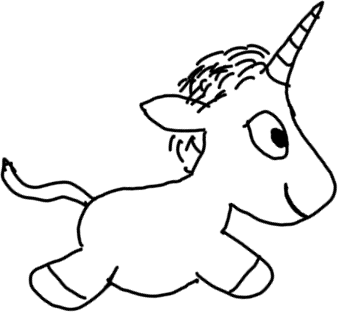
\includegraphics[scale=0.25]{UnicornDad.png}
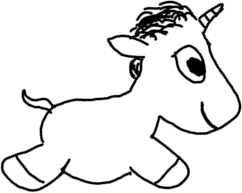
\includegraphics[scale=0.35]{UnicornChild.png}

\includegraphics[scale=0.3]{UnicornMom.png}

	\vfill\vfill
 
{\LARGE \textsf{Matthias Heizmann}}

\textsf{\footnotesize heizmann@informatik.uni-freiburg.de}

	\vfill\vfill
	
	{\large {\text{WS 2018/19}}}
	
	{Uni Freiburg}
	
	\vfill\vfill
	
	{\small\sffamily Zuletzt aktualisiert: \today}
\end{titlepage}

\subsection*{Zur Geschichte dieses Skriptes}

Das Skript wurde von Ralph Lesch begonnen und war zunächst ein Vorlesungsmitschrieb der im WS 2015/16 von Prof. Dr. Peter Thiemann gehaltenen Vorlesung.\\
\url{https://proglang.informatik.uni-freiburg.de/teaching/info3/2015ws/}

Für die im WS 2016/17 von Prof. Dr. Peter Thiemann gehaltene Vorlesung wurde das Skript von diesem und Luminous Fennell überarbeitet.\\
\url{https://proglang.informatik.uni-freiburg.de/teaching/info3/2016ws/}

Für die im WS 2017/18 von Dr. Matthias Heizmann gehalten Vorlesung wurde das Skript von diesem und Christian Schilling überarbeitet.\\
\url{http://swt.informatik.uni-freiburg.de/teaching/WS2017-18/info3}

Im WS 2018/19 wurde die Vorlesung erneut von Dr. Matthias Heizmann gehalten und das Skript nochmals überarbeitet.\\
\url{http://swt.informatik.uni-freiburg.de/teaching/WS2018-19/info3}

\smallskip

Trotz der vielen Bearbeitungsschritte ist dieses Skript noch nicht ``fertig''. Es soll kein eigenständiges Werk sondern eine Ergänzung zu den Vorlesungen sein.
Die Vorlesungen wurden großteils an der Tafel gehalten. Vereinzelt eingesetzte Folien sowie Übungsaufgaben und Klausuren sind auf den jeweiligen Vorlesungswebseiten verlinkt.

\smallskip

Der Latex Quellcode des Skriptes ist in einem Git Repositorium verfügbar.\\
\url{https://github.com/proglang/Informatik-III-Theoretische-Informatik}

\newpage

\vspace{\baselineskip}
\tableofcontents

\section[Vorspann: Sprachen]{Vorspann: Sprachen\datenote{19.10.2018}}
\begin{Def}[name={[Alphabet $\Sigma$]}]
	Ein \emph{Alphabet} ist eine endliche Menge von \emph{Zeichen}.
\end{Def} % 1.1
Zeichen sind hier beliebige abstrakte Symbole.

\newcommand{\aro}{\textit{rot}}
\newcommand{\age}{\textit{gelb}}
\newcommand{\agr}{\textit{grün}}

\begin{Bsp*} für Alphabete, die in dieser Vorlesung, im täglichem Umgang mit Computern oder in der Forschung an unserem Lehrstuhl eine Rolle spielen
  \begin{itemize}
  \item $\{a,\dots,z\}$
  \item $\{0, 1\}$
  \item $\{\aro, \age, \agr\}$ (Ampelfarben)
  \item Die Menge aller ASCII-Symbole
  \item Die Menge aller Statements eines Computerprogramms
  \qedhere
  \end{itemize}
\end{Bsp*}
Wir verwenden typischerweise den griechischen Buchstaben $\Sigma$ als Namen für ein Alphabet und die lateinischen Buchstaben $a,b,c$ als Namen für Zeichen.%
\footnote{Dies ist eine Konventionen analog zu den folgenden, die Sie möglicherweise in der Schule befolgten: Verwende $n,m$ für natürliche Zahlen. Verwende $\alpha, \beta$ für Winkel in Dreiecken. Verwende $A$ für Matrizen.}
Im Folgenden sei $\Sigma$ immer ein beliebiges Alphabet.%
\footnote{Dieser Satz dient dazu, dass die Autoren dieses Skripts nicht jede Definition mit ``Sei $\Sigma$ ein Alphabet...'' beginnen müssen.}

\begin{Def}[name={[Wort $w$ über $\Sigma$]}]\label{def:1.2}
  Wir nennen eine endliche Folge von Elementen aus $\Sigma$ ein \emph{Wort}
  und schreiben solch eine Folge immer ohne Trennsymbole wie z.B. Komma.\footnote{Wir schreiben also z.B. \texttt{einhorn} statt \texttt{e,i,n,h,o,r,n}.}
  Die leere Folge nennen wir das \emph{leere Wort}; als Konvention stellen wir das leere Wort mit dem griechischen Buchstaben $\Eps$ dar.\footnote{Eine analoge Konvention, die sie aus der Schule kennen: Verwende immer $\pi$ als Symbol für die Kreiszahl.}
  Wir bezeichnen die Menge aller Wörter mit $\Sigma^*$ und die Menge aller nicht leeren Wörter mit $\Sigma^+$.
  Die \emph{Länge} eines Wortes, $|\cdot| : \Sigma^* \to \N$, ist die Anzahl der Elemente der Folge.
\end{Def}
  Wir verwenden typischerweise $u,v,w$ als Namen für Wörter.

\goodbreak

\begin{Bsp*} für Wörter über $\Sigma=\{a,\dots,z\}$
  \begin{itemize}
  \item \verb/rambo/ (Länge $5$)
  \item \verb/eis/, \verb/ies/ (beide Länge 3 aber ungleich) 
  \item $\Eps$ (Länge $0$)
  \qedhere
  \end{itemize}
\end{Bsp*}
Wörter lassen sich "`verketten''/"`hintereinanderreihen''.
Die entsprechende Operation heißt \emph{Konkatenation}, geschrieben "`$\cdot$'' (wie Multiplikation).
\begin{Def}[Konkatenation von Wörtern]
  Die \emph{Konkatenation}, $\mathord{\cdot} : \Sigma^* \times \Sigma^* \to \Sigma^*$, ist für $u=u_1\ldots u_n\in\Sigma^*$ und $v=v_1\ldots v_m\in\Sigma^*$ definiert durch
  $u\cdot v = u_1\ldots u_nv_1\ldots v_m$
%   \begin{enumerate}
%   \item $\Eps\cdot v = v$ (leeres Wort ist linksneutrales Element)
%   \item $v\cdot \Eps = v$ (leeres Wort ist rechtsneutrales Element)
%   \item $u\cdot (v \cdot w) = (u\cdot v) \cdot w$ (Assoziativität)
%   \item $u(xw)\cdot v = ux(w\cdot v)$
%   \end{enumerate}
\end{Def}
% Punkt 2 (rechtsneutrales Element) folgt bereits aus 1. und 3. und könnte auch weggelassen werden.
\begin{Bsp*} ~
  \begin{itemize}
  \item $\mathtt{eis}\cdot\mathtt{rambo} =\mathtt{eisrambo}$
  \item $\mathtt{rambo} \cdot \Eps = \mathtt{rambo} = \Eps \cdot \mathtt{rambo}$ 
  \qedhere
  \end{itemize}
\end{Bsp*}
Eigenschaften von "`$\cdot$"':
\begin{itemize}
\item assoziativ
\item $\Eps$ ist neutrales Element
\item \emph{nicht} kommutativ
\end{itemize}


Der Konkatenationsoperator "`$\cdot$"' wird oft weggelassen (ähnlich wie der Multiplikationsoperator in der Arithmetik).
Ebenso können durch die Assoziativität Klammern weggelassen werden.
\begin{displaymath}
  w_1w_2w_3 \;\; \text{ steht also auch für } \;\; w_1\cdot w_2\cdot w_3,\;\;\text{ für }\;\;  (w_1 \cdot w_2) \cdot w_3 \;\;\text{ und für }\;\; w_1 \cdot (w_2 \cdot w_3)
\end{displaymath}

Bemerkung: Die Zeichenfolge \texttt{rambo}$\varepsilon$ ist \emph{kein} Wort.
Diese Zeichenfolge ist lediglich eine Notation für eine Konkatenationsoperation, die ein Wort der Länge 5 (nämlich \texttt{rambo}) beschreibt.

Wörter lassen sich außerdem \emph{potenzieren}:
\begin{Def}
  Die \emph{Potenzierung} von Wörtern, $\cdot ^ \cdot: \Sigma^*\times \N \to \Sigma^*$, ist induktiv definiert durch
  \begin{enumerate}
  \item $w^0 = \Eps$ 
  \item $w^{n+1} = w \cdot w^n$
  \qedhere
  \end{enumerate}
\end{Def}
\begin{Bsp*} $\mathtt{eis}^3 
\stackrel{(2.)}{=} \mathtt{eis}\cdot\mathtt{eis}^2 
\stackrel{\text{zweimal } (2.)}{=} \mathtt{eis}\cdot\mathtt{eis}\cdot\mathtt{eis}\cdot\mathtt{eis}^0
\stackrel{(1.)}{=} \mathtt{eis}\cdot\mathtt{eis}\cdot\mathtt{eis}\cdot\Eps
= \mathtt{eiseiseis}
$
\end{Bsp*}

\begin{Def}[name={[Sprache über $\Sigma$]}]
	Eine \emph{Sprache} über $\Sigma$ ist eine Menge $L\subseteq\Sigma^*$.
\end{Def}

\goodbreak

\begin{Bsp*}~ 
  \begin{itemize}
  \item 
	$\{\mathtt{eis}, \mathtt{rambo}\}$
  \item
    $\{w\in\{0,1\}^*\mid w \text{ ist Binärcodierung einer Primzahl}\}$
  \item $\{\}$ (die "`leere Sprache"')
  \item $\{ \Eps \}$ (ist verschieden von der leeren Sprache)
  \item $\Sigma^*$
  \qedhere
  \end{itemize}
\end{Bsp*}
Sämtliche Mengenoperationen sind auch Sprachoperationen, insbesondere Schnitt ($L_1 \cap L_2$), Vereinigung ($L_1 \cup L_2$), Differenz ($L_1 \setminus L_2$) und Komplement ($\overline{L_1} = \Sigma^* \setminus L_1$).

Weitere Operationen auf Sprachen sind Konkatenation und Potenzierung, sowie der \emph{Kleene-Abschluss}.
\begin{Def}[Konkatenation und Potenzierung von Sprachen] % 1.5
	Seien $U,V\subseteq \Sigma^*$. Dann ist die \emph{Konkatenation} von $U$ und $V$ definiert durch
	\[ U\cdot V = \{uv \mid u\in U, v\in V \} \]
  und die \emph{Potenzierung} von $U$ induktiv definiert durch
  \begin{enumerate}
  \item $U^0 = \{\Eps\}$
  \item $U^{n+1} = U \cdot U^{n}$
  \qedhere
  \end{enumerate}
\end{Def}
\begin{Bsp*}~
  \begin{itemize}
  \item $\{\mathtt{eis}, \Eps\} \cdot \{\mathtt{rambo}\} = \{\mathtt{eisrambo}, \mathtt{rambo}\}$
  \item $\{\mathtt{eis}, \Eps\} \cdot \{\} = \{\}$
  \item $\{\}^0 = \{\Eps\}$
  \item $\{\}^4 = \{\}$
  \item $\{\mathtt{eis}, \Eps\}^2 = \{\Eps, \mathtt{eis}, \mathtt{eiseis}\}$
  \qedhere
  \end{itemize}
\end{Bsp*}
Wie bei der Konkatenation von Wörtern dürfen wir den Konkatenationsoperator auch weglassen.
%
\begin{Def}[Kleene-Abschluss, Kleene-Stern, Kleene-Plus]
  Gegeben eine Sprache $U\subseteq\Sigma^*$, definieren wir den \emph{Kleene-Abschluss} $U^*$ wie folgt.
      $$U^* = \bigcup_{n\in\N} U^n$$
  Wie nennen den Operator $\cdot^*: \mathcal{P}(\Sigma^*)\rightarrow\mathcal{P}(\Sigma^*)$ der für eine gegebene Sprache den Kleene-Abschluss liefert den \emph{Kleene-Stern}. Analog definieren wir den \emph{Kleene-Plus} Operator $\cdot^+: \mathcal{P}(\Sigma^*)\rightarrow\mathcal{P}(\Sigma^*)$ als 
  $$U^+ = \bigcup_{n\ge1} U^n.$$
\end{Def}
Es gilt also $U^*=U^+\cup\{\Eps\}$.

%%% Local Variables:
%%% mode: latex
%%% TeX-master: "Info_3_Skript_WS2016-17"
%%% End:

\section[Reguläre Sprachen und endliche Automaten]{Reguläre Sprachen und endliche Automaten\datenote{20.10.17}}\label{sec:reglang}
Wie können wir potentiell unendlich große Mengen von Wörtern darstellen?
Eine Lösung für dieses Problem sahen wir bereits im vorherigen Kapitel, als wir die (unendlich große) Menge der binär codierten Primzahlen mit Hilfe der folgenden Zeile darstellten.
\[
L_\mathsf{prim}=\{w\in\{0,1\}^*\mid w \text{ ist Binärcodierung einer Primzahl}\}
\]
Ein weiteres Beispiel ist die folgende Zeile.
\[
L_\mathsf{even}=\{w\in\{0,1\}^*\mid \text{ die Anzahl der Einsen in $w$ ist gerade. }\}
\]
Eine häufig interessante Fragestellung für ein gegebenes Wort $w$ und eine Sprache $L$ ist: "`Ist $w$ in $L$ enthalten?"' (Also: "`Gilt $w\in L$?"')
Wir nennen dieses Entscheidunsproblem das \emph{Wortproblem}. Eine konkrete Instanz des Wortproblems wäre z.B.\ "`$1100101\in L_\mathsf{prim}$?"' oder "`$1100101\in L_\mathsf{even}$?"'

Die obige Darstellung der unendlichen Mengen $L_\mathsf{prim}$ und $L_\mathsf{even}$ ist zwar sehr kompakt, 
wir können daraus aber nicht direkt ein Vorgehen zur Lösung des Wortproblems ableiten.
Wir müssen zunächst verstehen, was die Begriffe "`Binärcodierung"', "`Primzahl"' oder "`gerade Anzahl"' bedeuten und für $L_\mathsf{prim}$ und $L_\mathsf{even}$ jeweils einen Algorithmus zur Entscheidung entwickeln.

In diesem Kapitel werden wir mit \emph{endlichen Automaten} einen weiteren Formalismus kennenlernen, um (potentiell unendlich große) Mengen von Wörtern darzustellen. 
Ein Vorteil dieser Darstellung ist, dass es einen einheitlichen und effizienten Algorithmus für das Wortproblem gibt.
Wir werden aber auch sehen, dass sich nicht jede Sprache (z.B.\ $L_\mathsf{prim}$) mit Hilfe eines endlichen Automaten darstellen lässt.

\subsection{Endliche Automaten}
Wir beschreiben zunächst informell die Bestandteile eines endlichen Automaten:

\newcommand{\qinit}{q^\mathsf{init}}
\newcommand{\B}{\mathcal{B}}
\newcommand{\calN}{\mathcal{N}}
\newcommand{\calP}{\mathcal{P}}
\newcommand{\ecl}{\textsf{ecl}}
\newcommand{\reach}{\textsf{reach}}
\renewcommand{\0}{\underline{\smash{\emptyset}}}
\renewcommand{\1}{\underline{\smash{\Eps}}}
\newcommand{\hide}[1]{}

\begin{description}
\item[Endliches Band] 
(read-only; jede Zelle enthält ein $a_i\in\Sigma$; der Inhalt des Bands ist das \emph{Eingabewort} bzw.\ die \emph{Eingabe})

\begin{figure}[H]\centering
        \begin{tikzpicture}
                \node (A) [block]{$a_0$};
                \node (B) [block,right=of A] {$\dots$};
                \node (C) [block,right=of B] {$a_n$};

    \node (L) [above=of A, node distance = 0.25cm] {Lesekopf};
    \draw[->] (L) -- (A);
        \end{tikzpicture}
        \caption{Endliches Band}
\end{figure}
\vspace{-1em}
\item[Lesekopf] ~\\
  \vspace{-\baselineskip}
  \begin{itemize}
        \item Der \emph{Lesekopf} zeigt auf ein Feld des Bands, oder hinter das letzte Feld.
        \item Er bewegt sich feldweise nach rechts; andere Bewegungen (Vor- bzw.\ Zurückspulen) sind nicht möglich.
        \item Wenn er hinter das letzte Zeichen zeigt, \emph{stoppt} der Automat.
    Er muss sich nun "`entscheiden"' ob er das Wort \emph{akzeptiert} oder nicht.
  \end{itemize}
\item[Zustände] $q$ aus \emph{endlicher} Zustandsmenge $Q$
\item[Startzustand] $\qinit \in Q$
\item[Akzeptierende Zustände] $F \subseteq Q$ 
\item[Transitionsfunktion] Im Zustand $q$ beim Lesen von $a$ gehe in Zustand $\delta(q) = q'$.
\end{description}
Der endliche Automat akzeptiert eine Eingabe, falls er in einem akzeptierenden Zustand stoppt.

% Spiral - By Keven Law - originally posted to Flickr as What's your Colour???, CC BY-SA 2.0, https://commons.wikimedia.org/w/index.php?curid=6851868
% Bunch - By Mariajudit - Own work, CC BY-SA 4.0, https://commons.wikimedia.org/w/index.php?curid=48726001
% Almond - By Michelle Naherny - Own work, CC BY-SA 4.0, https://commons.wikimedia.org/w/index.php?curid=44361114
\needspace{5\baselineskip}
\begin{Bsp}Aufgabe: 
  \\
  \label{Bsp:3.1}
  "`Erkenne alle Stapel von Macarons, in denen höchstens ein grünes Macaron vorkommt."'
\begin{center}
  \includegraphics[scale=0.4]{macaron-stacks.png}~\footnote{
  \tiny Von links nach rechts: \\
By Mariajudit - Own work, CC BY-SA 4.0, https://commons.wikimedia.org/w/index.php?curid=48726001
  \\
By Michelle Naherny - Own work, CC BY-SA 4.0, https://commons.wikimedia.org/w/index.php?curid=44361114
  \\
By Keven Law - originally posted to Flickr as What's your Colour???, CC BY-SA 2.0, \\ https://commons.wikimedia.org/w/index.php?curid=6851868
}
% Bunch - By Mariajudit - Own work, CC BY-SA 4.0, https://commons.wikimedia.org/w/index.php?curid=48726001
% Almond - By Michelle Naherny - Own work, CC BY-SA 4.0, https://commons.wikimedia.org/w/index.php?curid=44361114

\end{center}
Ein passendes Alphabet wäre $\Sigma = \{\texttt{grün} , \texttt{nicht-grün} \}$.
Wir definieren die folgenden Zustände.
(Die Metapher hier ist: "`wenn ich mehr als ein grünes Macaron esse, wird mir übel, und das wäre nicht akzeptabel"'.)
\begin{center}
\begin{tabular}{cl}
  Zustand & Bedeutung \\
  \hline
  $q_0$& "`alles gut"' \\
  $q_1$& "`mir wird schon flau"' \\
  $q_2$& "`mir ist übel"'
\end{tabular}
\end{center}
Der Startzustand ist $q_0$.
Akzeptierende Zustände sind $q_0$ und $q_1$.
Die Transitionsfunktion $\delta$ ist durch die folgende Tabelle gegeben.
\begin{center}
\begin{tabular}{cccl}
  &\texttt{grün} & \texttt{nicht-grün} \\
  \hline
  $q_0$ & $q_1$ & $q_0$ & wechsle nach $q_1$ falls \texttt{grün}, ansonsten verweile \\
  $q_1$ & $q_2$ & $q_1$ & wechsle nach $q_2$ falls \texttt{grün}, ansonsten verweile \\
  $q_2$  & $q_2$ & $q_2$ & verweile, da es nichts mehr zu retten gibt
\qedhere
\end{tabular}
\end{center}
\end{Bsp}

% \begin{Bsp}
%       $L=\{w\in\{0,1\}^* \mid w \text{ enthält gerade Anzahl von 0 und gerade Anzahl von 1}\}$

%       \begin{minipage}[t]{.4\textwidth}\centering\vspace{0pt}
%           \captionsetup{type=figure}
%               \begin{tikzpicture}[circle/.style={
%                       shape=circle,
%                       minimum size=0.5cm,
%                       text=black, draw,
%                       text width=0.5cm,
%                       align=center}]
%                       \node (v1) at (-3.5,3.5) {};
%                       \node [circle,double] (v2) at (-2.5,3) {$q_{00}$};
%                       \node [circle] (v3) at (0.5,3) {$q_{01}$};
%                       \node [circle] (v4) at (0.5,0.5) {$q_{10}$};
%                       \node [circle] (v5) at (-2.5,0.5) {$q_{11}$};
%                       \draw [->] (v1) edge (v2);
%                       \draw [->] (v2) edge [bend left=15] node[auto] {1} (v3);
%                       \draw [->] (v3) edge [bend left=15] node[auto] {1} (v2);
%                       \draw [->] (v3) edge [bend left=15] node[auto] {0} (v4);
%                       \draw [->] (v4) edge [bend left=15] node[auto] {0} (v3);
%                       \draw [->] (v2) edge [bend left=15] node[auto] {0} (v5);
%                       \draw [->] (v5) edge [bend left=15] node[auto] {0} (v2);
%                       \draw [->] (v5) edge [bend left=15] node[auto] {1} (v4);
%                       \draw [->] (v4) edge [bend left=15] node[auto] {1} (v5);
%               \end{tikzpicture}
%               \captionof{figure}{Automat zu $L$}
%       \end{minipage}\begin{minipage}[t]{.55\textwidth}\vspace{0pt}
%       Graphische Darstellung $\hat=$ gerichteter Graph mit Knoten $Q$ und markierten Kanten gemäß $\delta$.\\
%       $Q=\{q_{00},q_{01},q_{10},q_{11}\}$\\
%       $q_{00}$ einziger akzeptierender Zustand ($F=\{q_{00}\}$)
%       \end{minipage}
        
%       \begin{tabular}{M{l}|M{l}|M{l}l @{\quad}l}
%               & 0 & 1 &\\ \cline{1-3}
%               q_{00} & q_{10} & q_{01} && gerade Anzahl von 0 und 1 gesehen\\
%               q_{01} & q_{11} & q_{00} && gerade \ruleplaceholder{\widthof{Anzahl von 0}}, ungerade Anzahl von 1 gesehen\\
%               q_{10} & q_{00} & q_{11} && ungerade \ruleplaceholder{\widthof{Anzahl von 0}}, gerade \ruleplaceholder{\widthof{Anzahl von 1 gesehen}} \\
%               q_{11} & q_{01} & q_{10} && ungerade \ruleplaceholder{\widthof{Anzahl von 0}}, ungerade \ruleplaceholder{\widthof{Anzahl von 1 gesehen}}
%       \end{tabular}
% \end{Bsp}
\begin{Def}[\acs*{DEA}]
        Ein \emph{\acf{DEA}}, (\acsu{DFA} $\hat=$ \acl{DFA}) ist ein 5-Tupel
        \[ \A= (\Sigma, Q,\delta,\qinit,F). \]
Dabei ist
        \begin{itemize}
                \item $\Sigma$ ein Alphabet,
                \item $Q$ eine \emph{endliche} Menge, deren Elemente wir \emph{Zustände} nennen,
                \item $\delta:Q\x\Sigma\->Q$ eine Funktion, die wir \emph{Transitionsfunktion} nennen,
                \item $\qinit\in Q$ ein Zustand, den wir \emph{Startzustand} nennen und
                \item $F\subseteq Q$ eine Teilmenge der Zustände, deren Elemente wir \emph{akzeptierende} Zustände nennen.
                \qedhere
        \end{itemize}
\end{Def}

\acs*{DEA}s lassen sich auch graphisch darstellen.
Dabei gibt man für den Automaten einen gerichteten Graphen an.
Die Knoten des Graphen sind die Zustände, und mit Zeichen beschriftete Kanten zeigen, welchen Zustandsübergang die Transitionsfunktion für das nächste Zeichen erlaubt.
Der Startzustand ist mit einem unbeschrifteten Pfeil markiert, akzeptierende Zustände sind doppelt eingekreist.
Hier ist die graphische Darstellung von $A_{\mathtt{Macaron}}$ aus Beispiel~\ref{Bsp:3.1}:

\begin{center}
\begin{tikzpicture}[node distance = 3cm]
  \node[state, accepting] (0) {$q_0$};
  \node[state, accepting, right of = 0] (1) {$q_1$};
  \node[state, right of = 1] (2) {$q_2$};

  \node[left of = 0, node distance = 1cm] (start){}; 
  \draw[->] (start) to (0);

  \draw[->] (0) to node[above] {\texttt{grün}} (1);
  \draw[->, loop above] (0) to node[above] {\texttt{nicht-grün}} (0);

  \draw[->] (1) to node[above] {\texttt{grün}} (2);
  \draw[->, loop above] (1) to node[above] {\texttt{nicht-grün}} (1);

  \draw[->, loop right] (2) to node[right]{\texttt{grün}, \texttt{nicht-grün}} (2);
\end{tikzpicture}
\end{center}

% \acs*{DEA}s charakterisieren die Sprachen durch die Menge an Wörtern, die sie akzeptieren.
Die folgenden beiden Definitionen erlauben uns mit Hilfe eines \acs*{DEA} eine Sprache zu charakterisieren.
% \begin{Bsp}
%     Sei $M=(\Sigma, Q,\delta,q_0,F)$ ein \acs*{DEA}.
%     \begin{itemize}
%     \item Wenn $F=Q$, dann ist $L(M)=\Sigma^*$.
%     \item Wenn $F=\emptyset$, dann ist $L(M)=\emptyset$.
%     \end{itemize}
% \end{Bsp}
\begin{Def}[name={[Induktive erweiterung von $\delta$ auf Wörter]}]\label{def:2.deltaschlange}
        Die \emph{induktive Erweiterung} von $\delta:Q\x\Sigma\->Q$ auf Wörter, $\tilde{\delta}: Q\x\Sigma^*\->Q$, ist (induktiv) definiert durch
  \begin{enumerate}
  \item $\tilde\delta(q,\Eps) =q$\ \ \ \  (Wortende erreicht)
  \item $\tilde\delta(q,aw)=\tilde\delta(\delta(q,a),w)$\ \ \ \ (Rest im Folgezustand verarbeiten)
  \qedhere
  \end{enumerate}
\end{Def}
\begin{Def}[name={[Die durch einen \acs*{DEA} akzeptierte Sprache]}]\label{def:2.sprache}
        Sei $\A=(\Sigma, Q,\delta,\qinit,F)$. 
        Ein Wort $w\in\Sigma^*$ wird von $\A$ \emph{akzeptiert}, falls $\tilde\delta(\qinit,w)\in F$.
        Die \emph{von $\A$ akzeptierte Sprache}, geschrieben $L(\A)$, ist die Menge aller Wörter, die von $\A$ akzeptiert werden. D.h., 
        \[ L(\A) = \{ w\in\Sigma^* \mid \tilde\delta(\qinit,w)\in F \}. \]
        Eine durch einen \acs*{DEA} akzeptierte Sprache heißt \emph{regulär}.
\end{Def}

\begin{Bsp} 
\label{bsp:3.1} Ein möglicher \acs*{DEA} für die Sprache 
$$L_\mathsf{even}=\{w\in\{0,1\}^*\mid \text{ Die Anzahl der Einsen in $w$ ist gerade. }\}$$ 
aus der Einleitung dieses Kapitels hat die folgende graphische Repräsentation.
%         $L=\{w\in\{0,1\}^* \mid w \text{ enthält gerade Anzahl von 0 und gerade Anzahl von 1}\}$
  \begin{center}
                \begin{tikzpicture}[circle/.style={
                        shape=circle,
                        minimum size=0.5cm,
                        text=black, draw,
                        text width=0.5cm,
                        align=center}]
                        \node (v1) at (-3.5,3.5) {};
                        \node [circle,double] (v2) at (-2.5,3) {$q_{0}$};
                        \node [circle] (v3) at (0.5,3) {$q_{1}$};
                        \draw [->] (v1) edge (v2);
                        \draw [->] (v2) edge [bend left=15] node[auto] {1} (v3);
                        \draw [->] (v3) edge [bend left=15] node[auto] {1} (v2);
%                         \draw [->] (v1) edge [bend left=15] node[auto] {0} (v1);
%                         \draw [->] (v2) edge [bend left=15] node[auto] {0} (v1);
                        \draw [->] (v2) edge [loop below] node[auto] {0} (v2);
                        \draw [->] (v3) edge [loop below] node[auto] {0} (v3);
                \qedhere
                \end{tikzpicture}
  \end{center}
\end{Bsp}



% Es folgen zwei Beispiele für reguläre Sprachen:
% \begin{Bsp} 
% \label{bsp:3.1}
%         $L=\{w\in\{0,1\}^* \mid w \text{ enthält gerade Anzahl von 0 und gerade Anzahl von 1}\}$
%   \begin{center}
%                 \begin{tikzpicture}[circle/.style={
%                         shape=circle,
%                         minimum size=0.5cm,
%                         text=black, draw,
%                         text width=0.5cm,
%                         align=center}]
%                         \node (v1) at (-3.5,3.5) {};
%                         \node [circle,double] (v2) at (-2.5,3) {$q_{00}$};
%                         \node [circle] (v3) at (0.5,3) {$q_{01}$};
%                         \node [circle] (v4) at (0.5,0.5) {$q_{10}$};
%                         \node [circle] (v5) at (-2.5,0.5) {$q_{11}$};
%                         \draw [->] (v1) edge (v2);
%                         \draw [->] (v2) edge [bend left=15] node[auto] {1} (v3);
%                         \draw [->] (v3) edge [bend left=15] node[auto] {1} (v2);
%                         \draw [->] (v3) edge [bend left=15] node[auto] {0} (v4);
%                         \draw [->] (v4) edge [bend left=15] node[auto] {0} (v3);
%                         \draw [->] (v2) edge [bend left=15] node[auto] {0} (v5);
%                         \draw [->] (v5) edge [bend left=15] node[auto] {0} (v2);
%                         \draw [->] (v5) edge [bend left=15] node[auto] {1} (v4);
%                         \draw [->] (v4) edge [bend left=15] node[auto] {1} (v5);
%                 \end{tikzpicture}
%   \end{center}
% \end{Bsp}
% \begin{Bsp}\label{bsp:3.2}
%         
%         Sei $A\ge 0$ nat. Zahl, $\Sigma=\{0,1,\dots,A\}$
%         \begin{equation*}
%                 L = \{ a_1\dots a_n \mid \exists J\subseteq \{1,\dots,n \}: \sum_{i\in J} a_i = A \} \subseteq \Sigma^* 
%         \end{equation*}
%         D.h.\ gegeben eine Liste von Zahlen $\in\Sigma$.
%         Akzeptiere diejenigen Listen, für die eine Teilliste existiert, deren Summe genau $A$ ist.
%         \begin{align*}
%                 Q &=\Powerset\{0,1,\dots,A\} \\
%                 \delta(q,a) &= q \cup \{ x\in \{0,\dots,A\} \mid x-a \in q \} \\
%                 q_0 &=\{0\} \\
%                 F &= \{ q\in Q \mid A \in q \}
%         \end{align*}
%   $q \in Q$ bezeichnet die Menge an möglichen Summen $\le A$, die mit den bisher gelesenen Zeichen gebildet werden kann.
%   Die Transitionsfunktion $\delta$ fügt die Summen zum aktuellen Zustand hinzu, die sich durch addieren der aktuell gelesenen Ziffer zu den alten Möglichkeiten ergeben.
% \end{Bsp}
% \begin{Bsp}\label{bsp:3.3}
%         Beispiel für eine nicht-reguläre Sprache.
%         \begin{equation*}
%                 L = \{ 0^n1^n \mid n\in\N \} 
%         \end{equation*}
%         erkennbar durch \ac{TM} die immer anhält, \emph{aber nicht} von einem \ac{DEA} [\emph{nicht} regulär] akzeptiert werden kann.
%         \begin{proof}
%                 Angenommen $L=L(M)$ für \ac{DEA} $M=(\Sigma, Q,q_0,\delta,F)$
%                 
%                 Beobachtung: $\exists m\neq n$, sodass $\tilde\delta(q_0,0^m)=\tilde\delta(q_0,0^n)=q'$ weil $Q$ endlich.
%                 \begin{itemize}
%                         \item Falls nun $\tilde\delta(q',1^m)\in F$, dann ist auch $\tilde\delta(q_0,0^n1^m)\in F$ und somit $0^n1^m\in L(M)$ mit $n\neq m\ \lightning$
%                         \item Falls $\tilde\delta(q',1^m)\notin F$, dann gilt auch $\tilde\delta(q_0,0^m1^m)\notin F$ und somit $0^m1^m \notin L$ $\lightning$
%                 \end{itemize}
%                 Also kann $M$ nicht existieren!
%         \end{proof}
% \end{Bsp}

\datenote{24.10.18}
Frage: Angenommen wir haben zwei \ac{DEA}s $A_1$ und $A_2$, können wir dann immer einen \ac{DEA} konstruieren der den Schnitt $L(A_1)\cap L(A_2)$ akzeptiert?

Idee: Lasse beide \ac{DEA}s parallel laufen, akzeptiere nur wenn beide \ac{DEA}s akzeptieren.

Frage: Lassen sich zwei \emph{parallel laufende} \ac{DEA}s in einem einzigen \ac{DEA} implementieren?

Die nächste Konstruktion und der drauf folgende Satz liefern eine positive Antwort auf diese Frage.

\begin{Def}[Produktautomat für Schnitt]\label{def:2.Produktautomat}
Seien $A_1=(\Sigma, Q_1,\delta_1,\qinit_1,F_1)$ und $A_2=(\Sigma, Q_2,\delta_2,\qinit_2,F_2)$ \ac{DEA}s.
Wir definieren den \emph{Produktautomaten für Schnitt} als den \ac{DEA} $A_\cap=(\Sigma, Q_\cap,\delta_\cap,\qinit_\cap,F_\cap)$ mit den folgenden Komponenten.
		\begin{align*}
			Q_\cap &= Q_1\x Q_2\\
			\delta_\cap((q_1,q_2),a) &= (\delta_1(q_1,a),\delta_2(q_2,a))\;, \quad \text{für alle } a\in\Sigma\\
			\qinit_\cap &= (\qinit_1,\qinit_2)\\
			F_\cap &= F_1\x F_2\qedhere
		\end{align*}
\end{Def}

{\color{green!60!black}
\begin{Bemerkung}
In der Vorlesung vom 24.10.2018 wurde zunächst das Beispiel und dann erst die Konstruktion präsentiert.
\end{Bemerkung}
}

Im folgenden Beispiel sei $A_1$ der \ac{DEA} über dem Alphabet $\Sigma=\{0,1\}$, dessen graphische Repräsentation nahezu mit $A_{\mathtt{Macaron}}$ identisch ist.

\begin{center}
\begin{tikzpicture}[node distance = 3cm]
  \node[state, accepting] (0) {$q_0$};
  \node[state, accepting, right of = 0] (1) {$q_1$};
  \node[state, right of = 1] (2) {$q_2$};

  \node[left of = 0, node distance = 1cm] (start){}; 
  \draw[->] (start) to (0);

  \draw[->] (0) to node[above] {$1$} (1);
  \draw[->, loop above] (0) to node[above] {$0$} (0);

  \draw[->] (1) to node[above] {$1$} (2);
  \draw[->, loop above] (1) to node[above] {$0$} (1);

  \draw[->, loop right] (2) to node[right]{$1$, $0$} (2);
\end{tikzpicture}
\end{center}


\begin{Bsp}\label{bsp:2.schnitt}
Der Produktautomat für Schnitt von $A_1$ und $A_\mathsf{even}$ hat die folgende graphische Repräsentation, wobei wir um Platz zu sparen "`$q_{ij}$"' statt "`$(q_i, q_j)$"' schreiben.

\begin{center}
\begin{tikzpicture}[node distance = 3cm]
  \node[state, accepting] (00) {$q_{00}$};
  \node[state, accepting, right of = 00] (10) {$q_{10}$};
  \node[state, right of = 10] (20) {$q_{20}$};
  \node[state, below of = 00] (01) {$q_{01}$};
  \node[state, below of = 10] (11) {$q_{11}$};
  \node[state, below of = 20] (21) {$q_{21}$};

  \node[left of = 0, node distance = 1cm] (start){}; 
  \draw[->] (start) to (00);

  \draw[->, pos=0.3] (00) to node[above] {$1$} (11);
  \draw[->, pos=0.3] (01) to node[below] {$1$} (10);
  \draw[->, loop above] (00) to node[above] {$0$} (00);
  \draw[->, loop below] (01) to node[below] {$0$} (01);

  \draw[->, pos=0.3] (10) to node[above] {$1$} (21);
  \draw[->, pos=0.3] (11) to node[below] {$1$} (20);
  \draw[->, loop above] (10) to node[above] {$0$} (10);
  \draw[->, loop below] (11) to node[below] {$0$} (11);

  \draw[->,bend left] (20) to node[right] {$1$} (21);
  \draw[->,bend left] (21) to node[right] {$1$} (20);
  \draw[->, loop above] (20) to node[above]{$0$} (20);
  \draw[->, loop below] (21) to node[below]{$0$} (21);
\end{tikzpicture}
\end{center}
\end{Bsp}
{\color{green!60!black}
\begin{Bemerkung}
In der Vorlesung vom 24.10.2018 wurde das gleiche Beispiel mit vertauschten Operanden präsentiert. 
(Die resultierende Graphstruktur war also identisch aber die Beschriftung der Knoten war eine andere.)
\end{Bemerkung}
}



\begin{Satz}\label{satz:2.Produktautomat}
  Für beliebige \ac{DEA}s $A_1$ und $A_2$ akzeptiert der entsprechende Produktautomat für Schnitt die Sprache $L(A_1)\cap L(A_1)$.
%   Reguläre Sprachen sind abgeschlossen unter der Schnittoperation. (D.h.\ für zwei gegebene reguläre Sprachen $L_1$, $L_2$ über $\Sigma$ ist auch der Schnitt $L_1\cap L_2$ eine reguläre Sprache.)
\end{Satz}



% \begin{Satz}\label{satz:2.ClosedIntersection}
%   Reguläre Sprachen sind abgeschlossen unter der Schnittoperation. (D.h.\ für zwei gegebene reguläre Sprachen $L_1$, $L_2$ über $\Sigma$ ist auch der Schnitt $L_1\cap L_2$ eine reguläre Sprache.)
% \end{Satz}

% Der folgende Beweis ist ein typi

\begin{proof}\footnote{Dieser erste Beweis ist außergewöhnlich detailliert. In den folgenden Beweisen werden wir einfache Umformungen zusammenfassen.}
Seien $A_1=(\Sigma, Q_1,\delta_1,\qinit_1,F_1)$ und $A_2=(\Sigma, Q_2,\delta_2,\qinit_2,F_2)$ \ac{DEA}s und
$A_\cap=(\Sigma, Q_\cap,\delta_\cap,\qinit_\cap,F_\cap)$ der zugehörige Produktautomat für Schnitt.
Wir zeigen zunächst via Induktion über die Länge von $w$, dass für alle $w\in\Sigma^*$, für alle $q_1\in Q_1$ und für alle $q_2\in Q_2$ die folgende Gleichung gilt.
$$\tilde{\delta}_\cap((q_1,q_2),w) = (\tilde{\delta}_1(q_1,w), \tilde{\delta}_2(q_2,w))$$
Der Induktionsanfang für $n=0$ folgt dabei direkt aus \autoref{def:2.deltaschlange}, da $\Eps$ das einzige Wort der Länge $0$ ist.
$$\tilde{\delta}_\cap((q_1,q_2),\Eps) = (q_1,q_2)$$
Den Induktionsschritt $n\rightsquigarrow n+1$ zeigen wir mit Hilfe der folgenden Umformungen, wobei $a\in\Sigma$ ein beliebiges Zeichen und $w\in\Sigma^n$ ein beliebiges Wort der Länge $n$ ist.
\begin{eqnarray*}
  \tilde{\delta}_\cap((q_1,q_2),aw) 
    & \stackrel{\text{\autoref{def:2.deltaschlange}}}{=} & \tilde{\delta}_\cap(\delta_\cap((q_1,q_2),a),w)\\
    & \stackrel{\text{Def.\ }\delta_\cap}{=} & \tilde{\delta}_\cap (\big(\delta_1(q_1,a),\delta_2(q_2,a)\big),w)\\
    & \stackrel{\text{I.V.}}{=} & \big(\tilde{\delta}_1 (\delta_1(q_1,a),w), \tilde{\delta}_2(\delta_2(q_2,a),w)\big)\\
    & \stackrel{\text{\autoref{def:2.deltaschlange}}}{=} & \big(\tilde{\delta}_1(q_1,aw), \tilde{\delta}_2(q_2,aw)\big)
\end{eqnarray*}
Schließlich zeigen wir $L(A_\cap)=L(A_1)\cap L(A_2)$ mit Hilfe der folgenden Umformungen für ein beliebiges $w\in\Sigma^*$.
\begin{eqnarray*}
  w\in L(A_\cap)
  & \stackrel{\text{\autoref{def:2.sprache}}}{\mathsf{gdw}} & \tilde{\delta}_\cap(\qinit_\cap,w)\in F_\cap\\
  & \stackrel{\text{Def.\ }\qinit_\cap}{\mathsf{gdw}} & \tilde{\delta}_\cap((\qinit_1,\qinit_2),w)\in F_\cap\\
  & \stackrel{}{\mathsf{gdw}} & (\tilde{\delta}_1(\qinit_1,w),\tilde{\delta}_2(\qinit_2,w))\in F_\cap\\
  & \stackrel{\text{Def.\ }F_\cap}{\mathsf{gdw}} & \tilde{\delta}_1(\qinit_1,w)\in F_1 \text{ und } \tilde{\delta}_2(\qinit_2,w)\in F_2\\
  & \stackrel{\text{\autoref{def:2.sprache}}}{\mathsf{gdw}} & w\in L(A_1) \text{ und } w\in L(A_2)
\end{eqnarray*}
\end{proof}




\goodbreak





\subsection{Minimierung endlicher Automaten}
%  \datenote{26.10.16}

% Betrachte den Automaten aus Beispiel~\ref{bsp:3.2}.
% Sei $A =4$, $\Sigma = \{0, 1, 2, 3, 4\}$ mit Zustandsmenge $Q = \Powerset(\Sigma)$.
% D.h.\ unter anderem: $\{0, 1, 3\} \in Q$.
% Hier ist ein Ausschnitt aus dem Zustandsdiagramm:
% 
% \begin{center}
% \begin{tikzpicture}[node distance = 2cm]
%   \node (0) at (0, 0) {$\{0\}$};
%   \node[below of = 0] (03) {$\{0,3\}$};
%   \node[right of = 03] (02) {$\{0,2\}$};
%   \node[below of = 02] (0134) {$\{0,1,3,4\}$};
%   \node[right of = 0] (01) {$\{0,1\}$};
%   \node[right of = 01] (012) {$\{0,1,2\}$};
%   \node[below of = 012] (0123) {$\{0,1,2, 3\}$};
% 
%    \draw[->] (- 0.8, 0) to (0);
%   \draw[->] (0) to node[left] {$3$} (03);
%   \draw[->] (0) to node[above] {$2$} (02);
%   \draw[->] (0) to node[above] {$1$} (01);
%   \draw[->] (03) to node[left] {$1$} (0134);
%   \draw[->] (01) to node[above] {$1$} (012);
%   \draw[->] (02) to node[above] {$1$} (0123);
% \end{tikzpicture}
% \end{center}
% Es ist zu bemerken, dass manche Zustände von $Q$ nie erreicht werden können, z.B.\ $\emptyset$.
% Sei für die folgenden Überlegungen $M = (Q, \Sigma, \delta, \qinit, F)$ ein \acs*{DEA}.

Beobachtung: Der Zustand $q_{01}$ im Beispiel~\ref{bsp:2.schnitt} scheint nutzlos. Wir charakterisieren diese "`Nutzlosigkeit"' formal wie folgt.

\begin{Def}
  Ein Zustand $q \in Q$ heißt \emph{erreichbar}, falls ein $w \in \Sigma^*$ existiert, sodass $\hat \delta(\qinit, w) = q$.
%   $M$ heißt \emph{reduziert}, falls alle Zustände erreichbar sind.
\end{Def}
% \begin{Satz}
%   Die Menge der erreichbaren Zustände kann in $O(|Q|*|\Sigma|)$ berechnet werden.
% \end{Satz}
% \begin{proof}~\\
%   \vspace{-\baselineskip}
%   \begin{itemize}
%   \item Fasse $\A$ als Graphen auf.
%   \item Wende Tiefensuche an, markiere dabei alle besuchten Zustände.
%   \item Die markierten Zustände bilden die Menge der erreichbaren Zustände.
%   \end{itemize}
% \end{proof}
Bemerkung: Die Menge der erreichbaren Zustände kann mit dem folgenden Verfahren in $O(|Q|*|\Sigma|)$ berechnet werden.
  \begin{itemize}
  \item Fasse $\A$ als Graph auf.
  \item Wende Tiefensuche an und markiere dabei alle besuchten Zustände.
  \item Die markierten Zustände bilden die Menge der erreichbaren Zustände.
  \end{itemize}


% \ldots (TODO: hier fehlt noch etwas)
% \datenote{28.10.16}

% \emph{Beobachtung:} Auch ein Automat mit lauter erreichbaren Zuständen muss nicht minimal sein.
% \begin{Bsp}\label{Bsp:3.4}\
%   \begin{center}
%                 \begin{tikzpicture}
%                         \node (start) at (-4,1.5) {};
%                         \node (q0) [circle,double] at (-3,1) {$\qinit$};
%                         \node (q1) [circle,double] at (-0.5,1) {$q_1$};
%                         \node (q2) [circle] at (2,1) {$q_2$};
%                         \node (q3) [circle] at (3.5,1) {$q_3$};
%                         \draw [->] (start) edge (q0);
%                         \draw [->] (q0) edge[loop above] node {0} (q0);
%                         \draw [->] (q0) edge node [auto] {1} (q1);
%                         \draw [->] (q1) edge[loop above] node {0} (q1);
%                         \draw [->] (q1) edge node [auto] {1} (q2);
%                         \draw [->] (q2) edge[loop above] node {1} (q2);
%                         \draw [->] (q2) edge[bend left] node [auto] {0} (q3);
%                         \draw [->] (q3) edge[bend left] node [auto] {1,0} (q2);
%                 \end{tikzpicture}\\
%               \end{center}
%         Dieser Automat erkennt die gleiche Sprache wie in~\eqref{bsp:3.1} ("`höchstens eine 1"'), hat nur erreichbare Zustände, aber mehr Zustände als in~\eqref{bsp:3.1}.
%         
%         \emph{Beobachtung:} Aber $q_2$ und $q_3$ verhalten sich gleich in dem Sinn, dass
%         \[ \forall w: \tilde\delta(q_2,w) \notin F\text{ und }\tilde\delta(q_3,w)\notin F \]
% \end{Bsp}
%
%\stepcounter{Def}
%

\medskip

Beobachtung: Auch nach dem Entfernen der nicht erreichbaren Zustände $q_{01}$ und $q_{10}$ scheint der \acs*{DEA} aus \autoref{bsp:2.schnitt} unnötig groß zu sein. Das Verhalten des \acs*{DEA} in den Zuständen $q_{11}$, $q_{20}$ und $q_{21}$ ist sehr ähnlich. 
Wir charakterisieren diese "`Ähnlichkeit"' formal wie folgt.

\begin{Def}[name={[Äquivalenz von \acs*{DEA}-Zuständen]}] %\rlnote{Def.-Num. überprüfen}
  Wir nennen zwei Zustände $p,q\in Q$ eines \ac{DEA} \emph{äquivalent}, geschrieben $p\equiv q$, falls
  \begin{displaymath}
  \forall w\in\Sigma^*: \tilde\delta(p,w)\in F \text{ gdw } \tilde\delta(q,w)\in F
  \qedhere
  \end{displaymath}
\end{Def}
%\stepcounter{lemma}

\begin{Bsp}
Für \autoref{bsp:2.schnitt} gilt: 
Die Zustände $q_{11}$, $q_{20}$ und $q_{21}$ sind paarweise äquivalent.
Die Zustände $q_{00}$ und $q_{10}$ sind äquivalent.
Keine weiteren Zustandspaare sind äquivalent.

Geschrieben als Menge von Paaren sieht die Relation $\equiv\;\subseteq Q\times Q$ also wie folgt aus:
\[
\{ \,
(q_{00}, q_{10}), (q_{10}, q_{00}), \,
(q_{11}, q_{20}), (q_{20}, q_{11}), \,
(q_{20}, q_{21}), (q_{21}, q_{20}), \,
(q_{21}, q_{11}), (q_{11}, q_{21}) \,
\}\qedhere
\]
\end{Bsp}

{\color{green!60!black}
\begin{Bemerkung}
Der folgende Exkurs war Thema von Vorbereitungsblatt 01 und wurde in der der Vorlesung vom 24.10.2018 wurde nur kurz besprochen.
\end{Bemerkung}
}


\subsubsection{Exkurs: Äquivalenzrelationen}
Sie haben Äquivalenzrelationen bereits in "`Mathematik II für Studierende der Informatik"'\footnote{\url{http://home.mathematik.uni-freiburg.de/junker/ss17/matheII.html}} kennengelernt.
Dieser kurze Exkurs wiederholt die für unsere Vorlesung relevanten Definitionen.
Sei $X$ eine beliebige Menge. Eine \emph{Relation} $R$ über $X$ ist eine Teilmenge des Produkts $X\times X$ (d.h.\ $R\subseteq X\times X$).

Eine Relation $R\subseteq X\times X$ heißt
\begin{itemize}
 \item \emph{reflexiv}, wenn $\forall x\in X$: $(x,x)\in R$, 
 \item \emph{symmetrisch}, wenn $\forall x, y\in X$: $(x,y)\in R \;\; \Rightarrow\;\; (y,x)\in R$, 
 \item \emph{transitiv}, wenn $\forall x, y, z\in X$: $(x,y)\in R \land (y,z)\in R\;\; \Rightarrow\;\; (x,z)\in R$.
\end{itemize}

\begin{Bsp} Im Folgenden interessieren wir uns nur Relationen, die alle drei Eigenschaften erfüllen, 
aber die folgenden Beispiele sollen helfen, sich mit diesen Eigenschaften vertraut zu machen.

\begin{center}
\begin{tabular}{lccc}
& reflexiv & symmetrisch & transitiv\\ \hline
"`gewinnt"' bei Schere, Stein, Papier & nein & nein & nein\\
$(\N, <)$ & nein & nein & ja\\
$(\N, \neq)$ & nein & ja & nein\\
die leere Relation & nein & ja & ja\\
$\{(a,b)\in\mathbb{Z}\times\mathbb{Z}\mid a-b\leq 3\}$ & ja & nein & nein\\
$(\N, \leq)$& ja & nein & ja\\
direkte genetische Verwandtschaft & ja & ja & nein\\
logische Äquivalenz von Formeln & ja & ja & ja
\end{tabular}
\end{center}
Bemerkung: Wir können kein Beispiel für eine nicht leere, symmetrische, transitive Relation finden, die nicht reflexiv ist.
Für nicht leere Relationen folgt Reflexivität bereits aus Symmetrie und Transitivität: 
$(a,b)\in R\stackrel{\text{sym}}{\Rightarrow} (b,a)\in R\stackrel{\text{trans}}{\Rightarrow} (a,a)\in R$.
\end{Bsp}

\begin{Def}
Eine Äquivalenzrelation $R$ ist eine Relation, die reflexiv, symmetrisch und transitiv ist.

Für eine Äquivalenzrelation~$R$ und ein $x\in X$ nennen wir die Menge $\{y\in X \mid (y, x) \in R\}$ die \emph{Äquivalenzklasse} von $x$
und verwenden die Notation $[x]_R$ für diese Menge.
Wenn aus dem Kontext klar ist, welche Relation gemeint ist, dürfen wir das Subskript $\cdot_R$ auch weglassen und schreiben nur $[x]$.

Wenn wir eine Äquivalenzklasse mit Hilfe der Notation $[x]_R$ beschreiben, nennen wir $x$ den \emph{Repräsentanten} dieser Äquivalenzklasse.

Wir nennen die Anzahl der Äquivalenzklassen von $R$ den \emph{Index} von $R$.
\end{Def}

Zwei Fakten über eine beliebige Äquivalenzrelation $R$ (ohne Beweis).
\begin{description}
 \item[Fakt 1] Die Äquivalenzklassen von $R$ sind paarweise disjunkt.
 \item[Fakt 2] Die Vereinigung aller Äquivalenzklassen ist die Menge $X$.
\end{description}

Hiermit endet der Exkurs zu Äquivalenzrelationen; wir wollen mit diesem Wissen die oben definierte Relation $\equiv\; \subseteq Q\times Q$ genauer analysieren.

\begin{lemma}[name={[$\equiv$ ist Äquivalenzrelation]}]\datenote{26.10.18} %\rlnote{Satz = Lemma-Nummer: 3.2 statt 3.1?}
        Die Relation "`$\equiv$"' ist eine \emph{Äquivalenzrelation}.
\end{lemma}
\begin{proof}

  Die Relation $\equiv$ ist offensichtlich reflexiv.
  Die Symmetrie und Transitivität von~$\equiv$ folgt aus der Symmetrie und Transitivität der logischen Interpretation von "`genau dann, wenn"' (gdw).
\end{proof}


\begin{Bsp} 
Für den \ac{DEA} aus \autoref{bsp:2.schnitt} hat die Relation $\equiv$ drei Äquivalenzklassen.%
\footnote{Den Zustand $q_{11}$ als Repräsentanten für die dritte Äquivalenzklasse zu wählen ist eine völlig willkürliche Entscheidung. 
Wir könnten genauso gut $q_{20}$ oder $q_{21}$ wählen.}
\begin{align*}
 [q_{00}] & = \{q_{00}, q_{10}\},\\
 [q_{01}] & = \{q_{01}\},\\
 [q_{11}] & = \{q_{11}, q_{20}, q_{21}\}
 \qedhere
\end{align*}
\end{Bsp}





Idee: "`Verschmelze"' alle Zustände aus einer Äquivalenzklasse zu einem einzigen Zustand.
Bedenken: Bei einem \ac{DEA} hat jeder Zustand hat für jedes Zeichen einen Nachfolger. 
Wenn wir Zustände verschmelzen, könnte es mehrere Nachfolger geben und das Resultat wäre kein wohldefinierter \ac{DEA} mehr.

Das folgende Lemma zeigt, dass unsere Bedenken nicht gerechtfertigt sind. 
Sind zwei Zustände äquivalent, so sind auch für jedes Zeichen ihre Nachfolger äquivalent.

% \draftnote{28.10.16}
% \eqref{bsp:3.1}:
% \begin{minipage}{.5\textwidth}
%     \captionsetup{type=figure}
%         \begin{tikzpicture}
%                 \node (start) at (-4,1.5) {};
%                 \node (q0) [circle,double] at (-3,1) {$\qinit$};
%                 \node (q1) [circle,double] at (-0.5,1) {$q_1$};
%                 \node (q2) [circle] at (2,1) {$q_2$};
%                 \draw [->] (start) edge (q0);
%                 \draw [->] (q0) edge[loop above] node {0} (q0);
%                 \draw [->] (q1) edge[loop above] node {0} (q1);
%                 \draw [->] (q2) edge[loop above] node {0,1} (q2);
%                 \draw [->] (q0) edge node [auto] {1} (q1);
%                 \draw [->] (q1) edge node [auto] {1} (q2);
%         \end{tikzpicture}
%         \captionof{figure}{Automat zu~\eqref{bsp:3.1}}
% \end{minipage}

\begin{lemma}
\label{eqn:delta-wohldefiniert}
Für alle $p,q\in Q$ gilt:
        \[
        p \equiv q \quad\=>\quad \forall a\in\Sigma: \delta(p,a)\equiv\delta(q,a)
        \qedhere
        \]
\end{lemma}
\begin{proof}
\begin{eqnarray*}
        p \equiv q  
        & \text{gdw} & \forall w\in\Sigma^*: \tilde\delta(p,w)\in F \<=> \tilde\delta(q,w) \in F\\
        & \text{gdw} & (p\in F \<=> q \in F) \land \forall a\in \Sigma: \forall w\in\Sigma^*:
        \tilde\delta(p,aw)\in F \<=> \tilde\delta(q,aw)\in F\\
        &\text{impliziert} &  \forall a\in\Sigma: \forall w\in\Sigma^*: \tilde\delta(\delta(p,a),w)\in F \<=> \tilde\delta(\delta(q,a),w)\in F\\
        & \text{gdw} & \forall a\in\Sigma: \delta(p,a)\equiv\delta(q,a)
        \qedherefixeqnarray
\end{eqnarray*}
\end{proof}
Wir formalisieren das "`Verschmelzen"' von Zuständen wie folgt.
\begin{Def}[name={[Äquivalenzklassenautomat]}]
        Der Äquivalenzklassenautomat $\A_\equiv=(Q_\equiv,\Sigma,\delta_\equiv,{\qinit}_\equiv,F_\equiv)$ zu einem \acs*{DEA} $\A=(Q,\Sigma,\delta,\qinit,F)$ ist bestimmt durch:
        \begin{align*}
                Q_\equiv &= \{[q]\mid q\in Q\} & \delta_\equiv([q],a) &= [\delta(q,a)]\\
                \qinit_\equiv &= [\qinit] & F_\equiv & =\{[q]\mid q\in F \}
                \qedhere
        \end{align*}
\end{Def}

\begin{Bsp}
Der Äquivalenzklassenautomat $\A_\equiv$ zum \ac{DEA} aus \autoref{bsp:2.schnitt} hat das folgende Zustandsdiagramm.
 % \eqref{bsp:3.1}:
\begin{center}
   \captionsetup{type=figure}
        \begin{tikzpicture}
                \node (start) at (-1.5,1.7) {};
                \node (q0) [circle] at (-3,1) {\hspace*{-1mm}$[q_{01}]$};
                \node (q1) [circle,double] at (-0.5,1) {\hspace*{-1mm}$[q_{00}]$};
                \node (q2) [circle] at (2,1) {\hspace*{-1mm}$[q_{11}]$};
                \draw [->] (start) edge (q1);
                \draw [->] (q0) edge[loop above] node {0} (q0);
                \draw [->] (q1) edge[loop above] node {0} (q1);
                \draw [->] (q2) edge[loop above] node {0,1} (q2);
                \draw [->] (q0) edge node [auto] {1} (q1);
                \draw [->] (q1) edge node [auto] {1} (q2);
            \qedhere
        \end{tikzpicture}
\end{center}
\end{Bsp}



\begin{Satz}[name={[Äquivalenzklassenautomat ist wohldefiniert]}]
        Der Äquivalenzklassenautomat ist wohldefiniert und $L(\A_\equiv)=L(\A)$.
\end{Satz}


\begin{proof}\ 
        \begin{enumerate}
                \item Wohldefiniert: Es gilt zu zeigen, dass $\delta_\equiv([q],a) =[\delta(q,a)]$ nicht abhängig von der Wahl des Repräsentanten $q\in [q]$ ist. Dies folgt direkt aus \autoref{eqn:delta-wohldefiniert}.
                \item $L(\A)=L(\A_\equiv)$:
                Zunächst zeigen wir via Induktion über die Länge von $w$, dass für alle $w\in\Sigma^*$ und alle $q\in Q$ die folgende Äquivalenz gilt.
                \[\tilde\delta(q,w)\in F \<=> \tilde\delta_\equiv([q],w)\in F_\equiv\]
                
                
                I.A. $(n=0,$ also $w=\Eps)$: $\tilde\delta(q,\Eps)=q\in F \<=> \tilde\delta_\equiv([q],\Eps)=[q]\in F_\equiv$\\
                I.S.: ($n\rightsquigarrow n+1$) \begin{align*}
                \tilde\delta(q,aw)\in F &\<==> \tilde\delta(\delta(q,a),w)\in F\\ &\xLeftrightarrow{I.V.} \tilde\delta_\equiv([\delta(q,a)],w)\in F_\equiv\\
                &\<==> \tilde\delta_\equiv(\delta_\equiv([q],a),w)\in F_\equiv\\
                &\<==> \tilde\delta_\equiv([q],a w)\in F_\equiv
                \end{align*}
                Mir Hilfe dessen zeigen wir nun $L(\A)=L(\A_\equiv)$. Sei $w\in\Sigma^*$.
                \begin{align*}
                 w\in L(\A)
                 & \<==> \tilde\delta(\qinit,w) \in F\\
                 & \<==> \tilde\delta_\equiv([\qinit],w) \in F_\equiv\\
                 & \<==> w\in L(\A_\equiv)
                 \qedhere
                \end{align*}
        \end{enumerate}
\end{proof}
In den Übungen werden wir ein Verfahren mit Laufzeit $O(|Q|^4\cdot |\Sigma|)$ zur Konstruktion des Äquivalenzklassenautomaten kennenlernen. Es gibt aber auch schnellere Verfahren. Mit dem Algorithmus von Hopcroft kann $\A_\equiv$ in $O(|Q||\Sigma|\log|Q|)$ erzeugt werden.

Wir werden später (\-> Satz von Myhill-Nerode) sehen, dass $\A_\equiv$ der kleinste \acs*{DEA} ist, der $L(\A)$ akzeptiert.

\begin{Def}[name={[Rechtskongruente Äquivalenzrelation]}]
        Eine Äquivalenzrelation $R\subseteq\Sigma^*\x\Sigma^*$ heißt \emph{rechtskongruent}, falls
        \[
        (u,v)\in R \quad\=>\quad \forall w\in\Sigma^*: (u\cdot w,v\cdot w) \in R.
        \qedhere
        \]
\end{Def}




\textbf{Motivation:}
Ist eigentlich jede Sprache regulär? 
Falls nein, wie können wir nicht-reguläre Sprachen finden?
Wie können wir beweisen dass eine Sprache nicht regulär ist?
In weiteren Verlauf dieses Unterkapitels wollen wir charakteristische Merkmale von reguläre Sprachen finden.
Die Idee dazu basiert auf den folgenden Überlegungen:

Angenommen, wir möchten für eine gegebene Sprache $L$ einen \ac{DEA} $\A$ konstruieren.
Angenommen, wir haben bereits einen ersten Entwurf gemacht und in diesem führen sowohl das Wort $u\in\Sigma^*$
als auch das Wort $v\in\Sigma^*$ in den Zustand $q_{42}$ (formal: $\tilde\delta(\qinit, u) = \tilde\delta(\qinit, v) = q_{42}$).
\begin{figure}[H]\centering
                \begin{tikzpicture}
                        \node (start) at (-1,0.5) {};
                        \node (q0) [circle] at (0,0) {$\qinit$};
                        \node (q42) [circle] at (8,0) {$q_{42}$};
                        \draw[->,decoration = {zigzag,segment length = 2mm, amplitude = 0.5mm},decorate] (q0) .. controls (2,1) .. (3,0.5) .. controls (4,1) .. node[auto] {$u$} (q42);
                        \draw[->,decoration = {zigzag,segment length = 2mm, amplitude = 0.5mm},decorate] (q0) .. controls (3,-1) .. node[below] {$v$} (4,-0.5) .. controls (7,-1) .. (q42);
                        \draw [->] (start) edge (q0);
%                         \draw [->] (q0) edge [loop above] node {0} (q0);
%                         \draw [->] (q0) edge node [auto] {1} (q1);
%                         \draw [->] (q1) edge [bend left] node [auto] {1} (q0);
%                         \draw [->] (q1) edge node [auto] {0} (q2);
%                         \draw [->] (q2) edge [bend left] node [auto] {0} (q1);
%                         \draw [->] (q2) edge [loop above] node {1} (q2);
                \end{tikzpicture}
	\caption{Schematische Darstellung eines \ac{DEA}, mit $\tilde\delta(\qinit, u) = \tilde\delta(\qinit, v) = q_{42}$}
\end{figure}
\begin{itemize}
 \item Angenommen, es gibt ein Wort $w\in\Sigma^*$, sodass die Äquivalenz $uw\in L \Leftrightarrow vw\in L$ nicht gilt.
 Dann wissen wir, dass unser Entwurf noch einen Fehler enthält und wir dafür sorgen müssen, 
 dass der \ac{DEA} nicht sowohl von $u$
 als auch von $v$ in $q_{42}$ überführt wird.
 \item Angenommen, es gilt für alle Wörter $w\in\Sigma^*$, dass $uw\in L\Leftrightarrow vw\in L$.
 Dann wissen wir, dass es eine gute Idee war, den Automaten mit $u$ und $v$ in den gleichen Zustand zu führen.
\end{itemize}
Angenommen, wir finden nicht nur für zwei Wörter $u,v$ ein Wort $w$, sodass die Äquivalenz $uw\in L \Leftrightarrow vw\in L$ nicht gilt,
sondern wir finden solch ein $w$ für jedes Paar aus einer unendlich großen Menge von Wörtern $U$.
\begin{center}
(Formal: $\forall u,v\in U: u\neq v \Rightarrow \exists w^{uv}\in\Sigma^*: \neg(uw^{uv}\in L \Leftrightarrow vw^{uv}\in L)$) 
\end{center}
Dann wissen wir, dass all unsere Reparaturversuche hoffnungslos sind,
denn der \ac{DEA} $\A$ bräuchte für jedes $u\in U$ einen eigenen Zustand.
Doch ein \ac{DEA} darf nur endlich viele Zustände haben.
Die Sprache $L$ kann also nicht regulär sein.

Im weiteren Verlauf des Unterkapitels werden wir genau diese Überlegungen formal ausarbeiten.


%\setcounter{Bsp}{5}
\begin{Def} %\rlnote{Bsp.-Num. überprüfen (3.6)}
  \label{Bsp:R_m}
        Für einen \ac{DEA} $\A$ definiere
        \[ R_\A = \{(u,v) \mid \tilde\delta(\qinit,u)=\tilde\delta(\qinit,v)\}. \]
        \begin{description}
                \item[Beobachtung 1] $R_\A$ ist eine Äquivalenzrelation.
                
                Dies folgt daraus, dass "`="' eine Äquivalenzrelation ist.
                \item[Beobachtung 2] $R_\A$ ist rechtskongruent. 
                
                Dies wird in den Übungen bewiesen.
                \item[Beobachtung 3] Wir haben pro Zustand, der von $\qinit$ erreichbar ist, genau eine Äquivalenzklasse.
                Der Index von $R_\A$ ist also die Anzahl der erreichbaren Zustände.
        \end{description}
        
        \medskip
        
        Für den \ac{DEA} aus \autoref{bsp:2.schnitt} hat $R_\A$ die folgenden Äquivalenzklassen.
        \begin{align*}
        [\Eps] &= \{0^n\mid n\in \N\}\\
        [1] &= \{0^n10^m\mid n,m\in \N\}\\
        [11] &= \{w\mid \text{Anzahl von Einsen in $w$ ist gerade und $\geq 2$}\}\\
        [111] &= \{w\mid \text{Anzahl von Einsen in $w$ ist ungerade und $\geq 2$}\}
        \qedhere
        \end{align*}
\end{Def}
\begin{Def}\datenote{31.10.18}
        Für eine Sprache $L\subseteq \Sigma^*$ ist die \emph{Nerode-Relation} wie folgt definiert.
        \[
        R_L = \{(u,v) \mid \forall w\in\Sigma^*: uw\in L \<=> vw\in L \}
        \qedhere
        \]
\end{Def}
\begin{description}
 \item[Beobachtung 1] Die Nerode-Relation ist eine Äquivalenzrelation.
 
 Dies folgt daraus, dass "`$\Leftrightarrow$"' (Biimplikation, "`genau dann, wenn"') eine Äquivalenzrelation ist.
 \item[Beobachtung 2] Die Nerode-Relation ist rechtskongruent.
                \begin{proof}
                Sei $(u,v)\in R_L$. Zeige $\forall w\in\Sigma^*: (uw,vw)\in R_L$.
                Wir führen diesen Beweis via Induktion über die Länge von $w$.\\
                I.A. ($n=0$) Für $w=\Eps$ ist $ (u\Eps,v\Eps)=(u,v)\in R_L$.\\
%                 I.S. Sei Aussage gezeigt für alle Wörter $w'$ mit $|w'| \le k$.\\
                I.S. ($n\rightsquigarrow n+1$) Betrachte mit $w=w'a$ ein beliebiges Wort der Länge $n+1$.
                Nach Induktionsvoraussetzung ist dann auch $(uw', vw') \in R_L $.
                \begin{eqnarray*}
		(uw',vw')\in R_L 
		& \stackrel{\text{Def.\ } R_L}{\text{gdw}} & \forall z\in\Sigma^*: uw'z\in L \<=> vw'z\in L\\
		& \stackrel{\text{zerlege } z=az'}{\text{impliziert}} & \forall a\in \Sigma, z'\in\Sigma^*: uw'az'\in L \<=> vw'az'\in L\\
		& \stackrel{\text{Def.\ } R_L}{\text{impliziert}} & (uw'a,vw'a)\in R_L
		\qedherefixeqnarray
	      \end{eqnarray*}
              \end{proof}
\end{description}

\begin{Bsp}
Sei $\Sigma=\{0,1\}$. Die Sprache $L=\{w\in\Sigma^*\mid \text{vorletztes Zeichen von $w$ ist } 1\}$ hat die folgenden Äquivalenzklassen bezüglich der Nerode-Relation.
        \begin{align*}
        [\Eps] &= \{w\mid w \text{ endet mit } 00 \} \cup \{\varepsilon, 0\}\\
        [1] &= \{w\mid w \text{ endet mit } 01 \} \cup \{1\}\\
        [10] &= \{w\mid w \text{ endet mit } 10 \}\\
        [11] &= \{w\mid w \text{ endet mit } 11 \}
        \qedhere
        \end{align*}
\end{Bsp}

\begin{Bsp}
      Für ein beliebiges Alphabet $\Sigma$ gilt:
      \begin{enumerate}
       \item Die Sprache $L=\{\Eps\}$ hat genau zwei Äquivalenzklassen bezüglich der Nerode-Relation.
      Eine Äquivalenzklasse ist $\{\Eps\}$, die andere ist $\Sigma^+$.
       \item Die Sprache $L=\{\}$ hat genau eine Äquivalenzklasse (nämlich $\Sigma^*$) bezüglich der Nerode-Relation.
       \qedhere
      \end{enumerate}
\end{Bsp}

\begin{Bsp}\label{bsp:2.centeredMyhillNerode}
Sei $\Sigma=\{0,1\}$. Die Sprache $L_\text{centered}=\{0^n10^n \mid n\in\N\}$ hat bezüglich der Nerode-Relation die folgende Menge von Äquivalenzklassen:
$$\{ [w'] \mid w' \text{ ist Präfix eines Worts } w\in L_\text{centered}\} \cup \{ [11] \}$$

Bemerkung 1: Die Äquivalenzklasse $[11]$ enthält alle Wörter, die kein Präfix eines Worts aus $L_\text{centered}$ sind.

Bemerkung 2: Nicht für alle Präfixe von Wörtern in $L_\text{centered}$ sind die zugehörigen Äquivalenzklassen paarweise verschieden. Es gilt z.B. $[01]=[0010]$.

Bemerkung 3: Für je zwei verschiedene $k\in\N$ sind die Äquivalenzklassen $[0^k1]$ verschieden. Es gibt also unendlich viele Äquivalenzklassen.
\end{Bsp}

{\color{violet}
\begin{Bsp*}\footnote{Dieses Beispiel wurde in der Vorlesung übersprungen.}
 Die Sprache $L=\{w \in \{a,b\}^* \mid \#_a(w) > \#_b(w)\}$ hat bezüglich der Nerode-Relation die folgende Menge von Äquivalenzklassen:%

 \[
 \{ [w] \mid  \#_a(w) - \#_b(w)=k, k\in\mathbb{Z} \}
 \qedhere
 \]
\end{Bsp*}
}


% Beispiel: Drei Sprachen $L_a, L_b$ und $L_c$ mit unterschiedlichem Index  (Anzahl an Äquivalenzklassen) bzgl. der Nerode-Relation:
% \begin{alignat*}{2}
%         &\begin{rcases}
%         L_a=\{\Eps\} & [\Eps]\equiv[\Eps]\\
%         w,v\in\Sigma^*,\ w,v\ne\Eps & [w]=[v]
%         \end{rcases} &\ &\text{Index}= 2\\
%         &L_b = \varnothing, L_c= \Sigma^* &&\text{Index}= 1
% \end{alignat*}
% Die Menge der Äquivalenzklassen der Nerode-Relation $R_{L_a}$ auf $L_a$ ist
% \[ L_a / R_{L_a} = \{ [\Eps], [w] \} \]

\begin{Satz}[Myhill und Nerode] % 3.4
        Für alle Sprachen $L\subseteq \Sigma^*$ sind die folgenden Aussagen äquivalent:
        \begin{enumerate}
                \item\label{itm:Nerode1} $L$ wird von einem \ac{DEA} akzeptiert.
                \item\label{itm:Nerode2} $L$ ist Vereinigung von Äquivalenzklassen einer rechtskongruenten Äquivalenzrelation mit \emph{endlichem} Index.
                \item\label{itm:Nerode3} Die Nerode-Relation $R_L$ hat \emph{endlichen} Index.
                \qedhere
        \end{enumerate}
\end{Satz}

% \datenote{2.11.16}
\begin{proof}
  Wir beweisen die paarweise Äquivalenz in drei Schritten:

  \begin{center}
    (1) \=> (2), \quad \mbox{(2) \=> (3)}\quad \text{und} \quad (3) \=> (1)
  \end{center}

        \paragraph{(1) \=> (2)} Sei $\A$ ein \ac{DEA} mit
  \begin{displaymath}
    L(\A)=\{w \mid \tilde\delta(\qinit,w)\in F \} = \bigcup_{q \in F} \{ w \mid \tilde\delta(\qinit,w) = q\}.
\end{displaymath}
%
Nun sind $\{ w \mid \tilde\delta(\qinit,w)=q \}$ genau die Äquivalenzklassen der Relation $R_\A$ aus \autoref{Bsp:R_m}, einer rechtskongruenten Äquivalenzrelation.
Der Index ist die Anzahl der erreichbaren Zustände und somit endlich: $\operatorname{\operatorname{Index}}(R_\A) \le |Q| < \infty$.
        
\paragraph{(2) \=> (3)} Sei $R$ einer rechtskongruente Äquivalenzrelation mit endlichem Index, sodass $L$ die Vereinigung von $R$-Äquivalenzklassen ist.
        
Es genügt zu zeigen, dass die Nerode-Relation $R_L$ eine Obermenge von $R$ ist.%
\footnote{
Zur Erklärung: Falls $R \subseteq R_L$, dann gilt $\operatorname{Index}(R) \ge \operatorname{Index}(R_L)$.
Intuitiv: Je mehr Elemente eine Äquivalenzrelation $R$ enthält, desto mehr Elemente sind bzgl.\ dieser Relation äquivalent, d.h.\ desto weniger unterschiedliche Äquivalenzklassen gibt es.
}
\begin{comment}
% Ausformulierter Beweis
Es folgt $u \in L \Leftrightarrow v \in L$, da $L$ aus Vereinigung von Äquivalenzklassen besteht. Da $R$ rechtskongruent ist, folgt für alle $w$:
\[ uw \in L \Leftrightarrow vw \in L \]
Das aber ist die Definition der Nerode-Relation, d.h.\ $(u, v) \in R_L$. Da wir $(u, v)$ beliebig gewählt haben, gilt somit: 
\[\text{\#Klassen($R_L$) $\leq$ \#Klassen($R$)}<\infty\]
\end{comment}
\begin{align*}
(u, v) \in R & \quad\Rightarrow\quad u \in L \Leftrightarrow v \in L \text{, \quad da $L$ Vereinigung von Äquivalenzklassen ist} \\
& \quad\Rightarrow\quad \forall w \in \Sigma^*: uw \in L \Leftrightarrow vw \in L \text{, \quad da $R$ rechtskongruent } \\
& \quad\Rightarrow\quad (u, v) \in R_L \text{, \quad nach Definition der Nerode-Relation}
\end{align*}
Es gilt also $R \subseteq R_L$ und somit $\operatorname{Index}(R_L) \leq \operatorname{Index}(R)<\infty$.


\paragraph{(3) \=> (1)}\datenote{02.11.18} Gegeben $R_L$, konstruiere $\A=(Q,\Sigma,\delta,\qinit,F)$
    \begin{itemize}
    \item $Q = \{ [w]_{R_L} \mid w\in \Sigma^* \}$ \quad endlich, da $\operatorname{Index}$($R_L$) endlich
    \item $\delta([w],a) = [wa]$ \quad wohldefiniert, da $R_L$ rechtskongruent
    \item $\qinit = [\Eps]$
    \item $F = \{ [w] \mid w\in L \}$
    \end{itemize}
    Wir wollen nun $L(\A)=L$ zeigen. Dafür beweisen wir zunächst via Induktion über die Länge von $w$ die folgende Eigenschaft.
        \begin{displaymath}
      \forall w\in\Sigma^* :
                        \forall v\in\Sigma^* : \tilde\delta([v],w) = [v\cdot w]
    \end{displaymath}
    I.A. $(w = \Eps)$: $\tilde\delta([v],\Eps) = [v]=[v\cdot\Eps]$
    
    I.S. Sei $w = aw'$ beliebiges Wort der Länge $n+1$.
      \begin{displaymath}
        \begin{array}{lcl}
        \tilde\delta([v],aw') &=& \tilde\delta(\delta([v],a),w') \\
                             &=& \tilde\delta([v\cdot a],w') \\
                             &\stackrel{\text{I.V.}}{=}&[v\cdot a\cdot w'] \\
                             &=& [v\cdot \underbrace{aw'}_{=w}]
        \end{array}
      \end{displaymath}

Nun zeigen wir $L(\A)=L$ wie folgt:
\begin{eqnarray*}
        w\in L(\A)
        & \text{gdw} & \tilde\delta([\Eps],w)\in F\\
        & \text{gdw} & [w]\in F, \quad \text{(via Induktion gezeigte Eigenschaft für $v=\Eps$)}\\
        & \text{gdw} & w\in L
        \qedherefixeqnarray
\end{eqnarray*}
\end{proof}
%
\setcounter{Korollar}{4}
\begin{Korollar}\label{kor:2.minAutomat}
        Der im Beweisschritt (3) \=> (1) konstruierte Automat $\A$ ist ein minimaler Automat (bzgl.\ der Zustandsanzahl) für eine reguläre Sprache $L$.
\end{Korollar}
\begin{proof}
        Sei $\A'$ ein \emph{beliebiger} \ac{DEA} mit $L(\A')=L$.
        
        Aus "`\ref{itm:Nerode1} {\=>} \ref{itm:Nerode2}"' wissen wir, dass $\operatorname{Index}(R_{\A'})\leq |Q'|$ gilt.
        
        Aus "`\ref{itm:Nerode2} \=> \ref{itm:Nerode3}"' wissen wir, dass $R_{\A'}\subseteq R_L$ und somit $\operatorname{Index}(R_L) \leq \operatorname{Index}(R_{\A'})$ gilt.
        
        In "`\ref{itm:Nerode3} \=> \ref{itm:Nerode1}"' definieren wir $A$, sodass $|Q|=\operatorname{Index}(R_L) \leq \operatorname{Index}(R_\A)\leq |Q'|$ gilt.
        
        Für einen beliebigen \acs*{DEA} $A'$ ist $|Q|$ also nie größer als $|Q'|$.
\end{proof}





\subsection[\acf{NEA}]{Nichtdeterministischer endlicher Automat (NEA)}
Aufgabe: Konstruiere für eine natürliche Zahl $n\in\N$ einen \acs*{DEA} für die folgende Sprache.
	\begin{align*}
		L_n &= \{ w\in\{0,1\}^* \mid \text{das $n$-letzte Symbol von $w$ ist 1} \}
	\end{align*}
Naiver Lösungsversuch:
	\begin{figure}[H]\centering
		\begin{tikzpicture}[>=stealth, shorten >=1pt,
				node distance=1.5cm, on grid, initial text=,
				every state/.style={minimum size=0pt,inner sep=0pt}
			]
			\node[state,initial] (q0) {};
			\node[state] (q1) [right of=q0] {};
			\node        (q2) [right of=q1] {\dots};
			\node[state,accepting] (q3) [right of=q2] {};
			\path[->]
				(q0) edge [loop above] node [auto] {$\Sigma$} ()
				     edge              node [auto] {1}        (q1)
				(q1) edge              node [auto] {$\Sigma$} (q2)
				(q2) edge              node [auto] {$\Sigma$} (q3)
			;
			\draw [thick, decoration={brace, mirror, raise=.3cm, amplitude=10pt}, decorate]
			    (q1.west) -- (q3.east)
			    node [pos=0.5,anchor=north,yshift=-0.65cm] {n};
		\end{tikzpicture}
		\caption{Nichtdeterministischer Automat für $L_n$}
		\label{fig:2.nletztesNea}
	\end{figure}
Problem: Das Zustandsdiagramm beschreibt keinen \acs*{DEA}:
Der Startzustand hat zwei ausgehende Kanten für $1$.

Untersuche die Sprache mit Hilfe der Nerode-Relation.
Beobachtung: Je zwei Wörter der Länge $n$ sind in unterschiedlichen Äquivalenzklassen.
Es gibt also mindestens $2^n$ Äquivalenzklassen; aus \autoref{kor:2.minAutomat} wissen wir, dass ein minimaler \acs*{DEA}, der $L_n$ akzeptiert, mindestens $2^n$ Zustände haben muss.

Idee: Definiere einen neue Art von Automaten, bei dem ein Zustand pro Zeichen mehrere Nachfolger haben darf.

% \begin{Bsp*} Mustererkennung\\
% 	kommt ein String (konsistent) in einem anderen vor?
% 	
% 	Gegeben: festes Wort $w$.\\
% 	Gesucht: Sprache aller Worte, in denen $w$ als Teilwort vorkommt.
% 	\begin{align*}
% 		L &= \{ v\in\Sigma^* \mid \exists u,x\in\Sigma^*: v=uwx \}\\
% 		\Sigma &= \{a,b,c\}\\
% 		& \text{konkretes Beispiel:}\\
% 		w &= abac
% 	\end{align*}
% 	\begin{figure}[tp]
% 	\centering
% 		\begin{tikzpicture}[>=stealth, shorten >=1pt,
% 				node distance=2cm, on grid, initial text=,
% 				every state/.style={minimum size=0pt,inner sep=0pt}
% 			]
% 			\node[state,initial] (q0) {};
% 			\node[state] (q1) [right of=q0] {};
% 			\node[state] (q2) [right of=q1] {};
% 			\node[state] (q3) [right of=q2] {};
% 			\node[state,accepting] (q4) [right of=q3] {};
% 			\path[->]
% 				(q0) edge [loop above]    node [auto]  {$b,c$}    ()
% 				     edge                 node [auto]  {$a$}      (q1)
% 				(q1) edge [loop above]    node [auto]  {$a$}      ()
% 				     edge [bend left]     node [auto]  {$c$}      (q0)
% 				     edge                 node [auto]  {$b$}      (q2)
% 				(q2) edge [bend left=50]  node [auto]  {$b,c$}    (q0)
% 				     edge                 node [auto]  {$a$}      (q3)
% 				(q3) edge                 node [auto]  {$c$}      (q4)
% 				     edge [bend right=70] node [above] {$a$}      (q1)
% 				     edge [bend right=40] node [above] {$b$}      (q2)
% 				(q4) edge [loop right]    node [auto]  {$\Sigma$} ()
% 			;
% 		\end{tikzpicture}
% 	\caption{\acs*{DEA} für $L$}
% 	\label{fig:dfa-teilwort}
% 	\end{figure}
% 	\hyperref[fig:dfa-teilwort]{Abbildung~\ref*{fig:dfa-teilwort}} enthält einen \ac{DEA} für die Sprache $L$. Beobachtung: nicht-trivial zu konstruieren.
% 	\begin{figure}[tp]\centering
% 		\begin{tikzpicture}[>=stealth,shorten >=1pt,
% 				node distance=2cm,on grid,
% 				initial text=
% 			]
% 			\node[state,initial] (q0) {$q_0$};
% 			\node[state] (q1) [right of=q0] {$q_1$};
% 			\node[state] (q2) [right of=q1] {$q_2$};
% 			\node[state] (q3) [right of=q2] {$q_3$};
% 			\node[state,accepting] (q4) [right of=q3] {$q_4$};
% 			\path[->]
% 				(q0) edge [loop above] node [auto] {$\Sigma$} ()
% 				     edge              node [auto] {$a$} (q1)
% 				(q1) edge              node [auto] {$b$} (q2)
% 				(q2) edge              node [auto] {$a$} (q3)
% 				(q3) edge              node [auto] {$c$} (q4)
% 				(q4) edge [loop above] node [auto] {$\Sigma$} ()
% 			;
% 		\end{tikzpicture}
% 		\caption{Bsp.: Mustererkennung}
% 		\label{fig:nfa-teilwort}
% 	\end{figure}
% 	
% 	\hyperref[fig:nfa-teilwort]{Abbildung~\ref*{fig:nfa-teilwort}} enthält einen nicht-deterministischen endlichen Automat für die Sprache $L$. Idee: Ein Wort $w$ wird akzeptiert, falls es einen mit $w$ markierten Pfad von $q_0$ zu einen akzeptierenden Zustand gibt.
% 	\begin{figure}[tp]
% 	\centering
% 		\begin{tikzpicture}[>=stealth,shorten >=1pt,
% 				node distance=2cm,on grid
% 			]
% 			\node (q0) {$\{0\}$};
% 			\node (q1) [right of=q0] {$\{0,1\}$};
% 			\node (q2) [right of=q1] {$\{0,2\}$};
% 			\node (q3) [right of=q2] {$\{0,1,3\}$};
% 			\path[->]
% 				(q0) edge [loop below] node [auto] {$b,c$} ()
% 				     edge              node [auto] {$a$} (q1)
% 				(q1) edge [loop below] node [auto] {$a$} ()
% 				(q1) edge              node [auto] {$b$} (q2)
% 				(q2) edge              node [auto] {$a$} (q3)
% 			;
% 		\end{tikzpicture}
% 	\caption{Potenzmengenkonstruktion auf dem \acs*{NEA}}
% 	\label{fig:nfa-teilwort-powerset}
% 	\end{figure}
% 	
% 	\hyperref[fig:nfa-teilwort-powerset]{Abbildung~\ref{fig:nfa-teilwort-powerset}} zeigt (einen Ausschnitt) aus dem deterministischen Automaten, der schematisch aus dem \acsu{NEA} in \autoref{fig:nfa-teilwort} konstruiert werden kann. Idee: bei Schritt mit Symbol $a$ ist der \ac{NEA} gleichzeitig in allen Zuständen, die durch $a$ von (der Menge der) aktuellen Zustände erreichbar sind.
% 	
% 	Variante: erkenne \textbf{Subwort} $w=a_1,\dots,a_n$
% 	\[ L' = \{ v\in\Sigma^* \mid \exists x_0,\dots,x_n\in\Sigma^*: v=x_0a_1x_1a_2\dots a_nx_n \} \]
% 	Nicht det. Automat für $L'$ mit $(w=abac)$ ist sehr einfach. Der entsprechende deterministische Automat ist deutlich komplizierter. (selbst)
% 	\begin{figure}[H]\centering
% 		\begin{tikzpicture}[>=stealth, shorten >=1pt,
% 				node distance=2cm, on grid, initial text=,
% 				every state/.style={minimum size=0pt,inner sep=0pt}
% 			]
% 			\node[state,initial] (q0) {};
% 			\node[state] (q1) [right of=q0] {};
% 			\node[state] (q2) [right of=q1] {};
% 			\node[state] (q3) [right of=q2] {};
% 			\node[state,accepting] (q4) [right of=q3] {};
% 			\path[->]
% 				(q0) edge [loop above] node [auto] {$\Sigma$} ()
% 				     edge              node [auto] {$a$}      (q1)
% 				(q1) edge [loop below] node [auto] {$\Sigma$} ()
% 				     edge              node [auto] {$b$}      (q2)
% 				(q2) edge [loop below] node [auto] {$\Sigma$} ()
% 				     edge              node [auto] {$a$}      (q3)
% 				(q3) edge [loop below] node [auto] {$\Sigma$} ()
% 				     edge              node [auto] {$c$}      (q4)
% 				(q4) edge [loop right] node [auto] {$\Sigma$} ()
% 			;
% 		\end{tikzpicture}
% 		\caption{Nichtdet. Automat für $L'$}
% 	\end{figure}
% 	
% 	Weiteres Beispiel, bei dem der deterministische Automat beweisbar exponentiell größer ist.
% 	\begin{align*}
% 		L_n &= \{ w\in\{0,1\}^* \mid \text{das $n$-letzte Symbol von $w$ ist 1} \}
% 	\end{align*}
% 	\begin{figure}[H]\centering
% 		\begin{tikzpicture}[>=stealth, shorten >=1pt,
% 				node distance=1.5cm, on grid, initial text=,
% 				every state/.style={minimum size=0pt,inner sep=0pt}
% 			]
% 			\node[state,initial] (q0) {};
% 			\node[state] (q1) [right of=q0] {};
% 			\node        (q2) [right of=q1] {\dots};
% 			\node[state,accepting] (q3) [right of=q2] {};
% 			\path[->]
% 				(q0) edge [loop above] node [auto] {$\Sigma$} ()
% 				     edge              node [auto] {1}        (q1)
% 				(q1) edge              node [auto] {$\Sigma$} (q2)
% 				(q2) edge              node [auto] {$\Sigma$} (q3)
% 			;
% 			\draw [thick, decoration={brace, mirror, raise=.3cm, amplitude=10pt}, decorate]
% 			    (q1.west) -- (q3.east)
% 			    node [pos=0.5,anchor=north,yshift=-0.65cm] {n};
% 		\end{tikzpicture}
% 		\caption{Nichtdet. Automat für $L_n$}
% 	\end{figure}
% 	
% 	Der entsprechende deterministische Automat für $L_n$ hat $\sim 2^n$ Zustände.
% \end{Bsp*}

\goodbreak

\begin{Def}[\acs*{NEA}]
        Ein \emph{\acf{NEA}}, (\acsu{NFA} $\hat=$ \acl{NFA}) ist ein 5-Tupel
        \[ \calN= (\Sigma, Q,\delta,\qinit,F). \]
Dabei ist
        \begin{itemize}
                \item $\Sigma$ ein Alphabet,
                \item $Q$ eine \emph{endliche} Menge, deren Elemente wir \emph{Zustände} nennen,
                \item $\delta:Q\x\Sigma\->\mathcal{P}(Q)$ eine Funktion, die wir \emph{Transitionsfunktion} nennen,
                \item $\qinit\in Q$ ein Zustand, den wir \emph{Startzustand} nennen und
                \item $F\subseteq Q$ eine Teilmenge der Zustände, deren Elemente wir \emph{akzeptierende} Zustände nennen.
                \qedhere
        \end{itemize}
\end{Def}
Bemerkung: Die Definition des \acs*{NEA} unterscheidet sich vom \acs*{DEA} also nur in der Transitionsfunktion. Beim \acs*{DEA} ist der Bildbereich der Transitionsfunktion die Menge der Zustände $Q$. Beim \acs*{NEA} ist der Bildbereich die Potenzmenge $\mathcal{P}(Q)$ der Zustandsmenge~$Q$.
Analog zu \acs*{DEA}s werden wir auch \acs*{NEA}s mit Hilfe eines Zustandsdiagramms beschrieben. Zum Beispiel beschreibt \autoref{fig:2.nletztesNea} für jedes $n\in\N$ einen \acs*{NEA} für die Sprache $L_n$.

Im Folgenden sei $\calN$ immer ein \acs*{NEA}.
\begin{Def}[name={[Lauf eines Automaten]}]
	Wir nennen eine Folge von Zuständen $q_0q_1\dots q_n$ einen \emph{Lauf von $\calN$ über $w=a_1\dots a_n$}, falls
	$q_i\in\delta(q_{i-1},a_i)$ für alle $i$ mit $1\leq i\leq n$.
	Wir nennen einen Lauf \emph{initial}, falls $q_0=\qinit$.
	Wir nennen einen Lauf \emph{akzeptierend}, falls $q_n\in F$.
\end{Def}
\begin{Def}[name={[NEA zu DEA]}]
	Ein Wort $w\in\Sigma^*$ wird von $\calN$ \emph{akzeptiert}, falls $\calN$ einen initialen und akzeptierenden Lauf über $w$ hat.
	Die von $\calN$ akzeptierte Sprache ist die Menge der von $\calN$ akzeptierten Wörter, d.h.\
	$L(\calN)=\{ w\in\Sigma^* \mid \exists\text{ initialer, akzeptierender Lauf von $\calN$ über }w \}$.
\end{Def}




\begin{Bsp}
\label{bsp:2.zweitletztes} Der \acs*{NEA} für die Sprache 
$$L_2=\{w\in\{0,1\}^*\mid \text{ das zweitletzte Zeichen von $w$ ist $1$ }\}$$ hat die folgende graphische Repräsentation.
  \begin{center}
                \begin{tikzpicture}[circle/.style={
                        shape=circle,
                        minimum size=0.5cm,
                        text=black, draw,
                        text width=0.5cm,
                        align=center}]
                        \node (vs) at (-1.0,1.0) {};
                        \node [circle] (v0) at (0,0) {$q_{0}$};
                        \node [circle] (v1) at (3,0) {$q_{1}$};
                        \node [circle, double] (v2) at (6,0) {$q_{2}$};
                        \draw [->] (vs) edge (v0);
                        \draw [->] (v0) edge [loop above] node[auto] {0,1} (v2);
                        \draw [->] (v0) edge [bend left=15] node[auto] {1} (v1);
                        \draw [->] (v1) edge [bend left=15] node[auto] {0,1} (v2);
                        \qedhere
                \end{tikzpicture}
  \end{center}
\end{Bsp}


Bemerkung: Die Frage, ob ein gegebenes Wort $w$ akzeptiert wird (das "`Wortproblem"'), lässt sich für \acs*{NEA}s nicht mehr so leicht beantworten wie wir es von \acs*{DEA}s gewohnt sind.
Ein sinnvolles Vorgehen scheint, jeden initialen Lauf zu betrachten, doch z.B.\ für das Wort $11$ hat obiger \acs*{NEA} bereits  drei verschiedene initiale Läufe: $q_0q_0q_0$, $q_0q_0q_1$ und $q_0q_1q_2$.


Bemerkung: Die Definitionen von \ac{NEA} und \ac{DEA} in der Literatur sind nicht einheitlich. 
Es gibt äquivalente \ac{NEA}-Definitionen, die statt der Transitionsfunktion $\delta:Q\x\Sigma\->\mathcal{P}(Q)$ eine Transitionsrelation $\delta\subseteq Q\x\Sigma\x Q$ verwenden.
Es gibt alternative \ac{NEA}-Definitionen, die eine Menge von Startzuständen erlauben.
Alternativ könnte man auch zunächst den \ac{NEA} einführen und den \ac{DEA} als Spezialfall dessen definieren (Spezialfall: Das Bild der Transitionsfunktion ist einelementig für alle $q\in Q$ und $a\in\Sigma$).

Bemerkung: Zu jedem \ac{DEA} $\A= (\Sigma, Q,\delta,\qinit,F)$ gibt es einen \ac{NEA}, der die gleiche Sprache akzeptiert.
Beispiel: der \ac{NEA} $\calN= (\Sigma, Q,\delta_\mathsf{NEA},\qinit,F)$ mit $\delta_\mathsf{NEA}(q,a)=\{\delta(q,a)\}$, der sich von $\A$ nur in der Transitionsfunktion unterscheidet.


\begin{Satz}[Rabin und Scott]\label{satz:2.rabinscott}
	Zu jedem \ac{NEA} $\calN$ mit $n$ Zuständen gibt es einen \ac{DEA} $\A_\calP$ mit $2^n$ Zuständen, sodass $L(\A_\calP)=L(\calN)$ gilt.
\end{Satz}
  Zur Vorbereitung des Beweises machen wir zunächst die folgende Definition.

\begin{Def}[Potenzmengenautomat]
 Für einen gegebenen \ac{NEA}  $\calN= (\Sigma, Q,\delta,\qinit,F)$ ist der Potenzmengenautomat $\A_\calP$ wie folgt definiert.
         \begin{align*}
                Q_\calP &= \mathcal{P}(Q)\\
                \delta_\calP(p,a) &= \bigcup_{q\in p} \{\delta(q,a)\}\\
                \qinit_\calP &= \{\qinit\}\\
                F_\calP &= \{ p\in Q_\calP \mid p\cap F\neq \varnothing \}
                \qedhere
        \end{align*}
\end{Def}
\begin{Bsp}
Der Potenzmengenautomat für den \acs*{NEA} aus \autoref{bsp:2.zweitletztes} hat das folgende Zustandsdiagramm.
  \begin{center}
                \begin{tikzpicture}[circle/.style={
                        shape=circle,
                        minimum size=0.5cm,
                        text=black, draw,
                        text width=0.5cm,
                        align=center}]
                        \node (vs) at (-1.0,1.0) {};
                        \node [draw, rounded corners=3mm] (v0) at (0,0) {$\{q_{0}\}$};
                        \node [draw, rounded corners=3mm] (v1) at (2,0) {$\{q_{0}, q_1\}$};
                        \node [draw, rounded corners=3mm, double] (v2) at (5,1) {$\{q_0, q_{2}\}$};
                        \node [draw, rounded corners=3mm, double] (v3) at (5,-1) {$\{q_0, q_1, q_2\}$};
                        \node [draw, rounded corners=3mm, double] (v4) at (8,1) {$\{q_1, q_2\}$};
                        \node [draw, rounded corners=3mm] (v5) at (12,1) {$\{q_1\}$};
                        \node [draw, rounded corners=3mm, double] (v6) at (10,1) {$\{q_2\}$};
                        \node [draw, rounded corners=3mm] (v7) at (10,-1) {$\{\}$};
                        \draw [->] (vs) edge (v0);
                        \draw [->] (v0) edge [loop above] node[auto] {0} (v2);
                        \draw [->] (v0) edge [bend left=0] node[below] {1} (v1);
                        \draw [->] (v1) edge [bend left=15] node[auto] {0} (v2);
                        \draw [->] (v1) edge [bend left=0] node[below] {1} (v3);
                        \draw [->] (v2) edge [bend right=30] node[above] {0} (v0);
                        \draw [->] (v2) edge [bend left=15] node[auto] {1} (v1);
                        \draw [->] (v3) edge [bend left=0] node[right] {0} (v2);
                        \draw [->] (v3) edge [loop right] node[auto] {1} (v3);
                        \draw [->] (v4) edge [] node[auto] {0,1} (v6);
                        \draw [->] (v5) edge [] node[auto,above] {0,1} (v6);
                        \draw [->] (v6) edge [] node[auto] {0,1} (v7);
                        \draw [->] (v7) edge [loop right] node[auto] {0,1} (v7);
                \end{tikzpicture}
  \end{center}
Die vier Zustände auf der rechten Seite sind nicht erreichbar.
\end{Bsp}


\draftnote{6.11.18}
\begin{proof}[von \autoref{satz:2.rabinscott}]
        Zeige $L(\A_\calP)=L(\calN)$. 
        Dafür beweisen wir zunächst via Induktion über die Länge von $w$ die folgende Eigenschaft:
        
        $\forall w\in\Sigma^*\; \forall p\in Q_\calP\backslash\{\{\}\}\; \forall q\in Q:$
        $$q\in\tilde\delta_\calP(p,w) \Leftrightarrow \exists \underbrace{q_0, q_1,\ldots, q_n}_{\text{Lauf}}\in Q, \text{ sodass }  n=|w|, q_0\in p \text{ und } q_n=q$$
        I.A. $(n=0,$ also $w=\Eps)$: Gilt trivialerweise, da $p\neq\{\}$.\\
        I.S. ($n\rightsquigarrow n+1$): Sei $w=aw'$ ein beliebiges Wort der Länge $n+1$.
        \begin{eqnarray*}
                q\in\tilde\delta_\calP(p,w) 
                \hspace*{-2.5mm} & \Leftrightarrow & \hspace*{-2.5mm} q\in\tilde\delta_\calP(\delta_\calP(p,a),w')\\
                & \stackrel{\text{I.V.}}{\Leftrightarrow} & \hspace*{-2.5mm} \exists\underbrace{q_1,q_2,\ldots, q_{n+1}}_{\text{Lauf}}\in Q, \text{ sodass }  n=|w'|, q_1\in \delta_\calP(p,a) \text{ und } q_{n+1}=q\\
                & \Leftrightarrow & \hspace*{-2.5mm}\exists\underbrace{q_1,q_2,\ldots, q_{n+1}}_{\text{Lauf}}\in Q, \text{ sodass }  n=|w'|, \exists q_0\in p: q_1\in\delta(q_0,a) \text{ und } q_{n+1}=q\\
                & \Leftrightarrow & \hspace*{-2.5mm} \exists\underbrace{q_0,q_1,q_2,\ldots, q_{n+1}}_{\text{Lauf}}\in Q,\text{ sodass }  n+1=|w|, q_0\in p \text{ und } q_{n+1}=q
        \end{eqnarray*}
        Mit Hilfe dieser Eigenschaft zeigen wir nun die Gleichheit $L(\A_\calP)=L(\calN)$.
        \begin{align*}
         w\in L(\A_\calP) 
         &\<=> \tilde\delta_\calP(\qinit_\calP,w)\in F_\calP\\
         &\<=> \exists q_f\in \tilde\delta_\calP(\qinit_\calP,w)\cap F\\
         &\<=> \exists \underbrace{q_0, q_1,\ldots, q_n}_{\text{Lauf}}\in Q, \text{ sodass }  n=|w|, q_0\in \qinit \text{ und } q_n\in F\\
         &\<=> \exists \text{ initialer, akzeptierender Lauf von $\calN$ über $w$} \\
         &\<=> w\in L(\calN)
         \qedhere
        \end{align*}
\end{proof}

Bemerkung: Es gelten also die folgenden Äquivalenzen.
\[
L \text{ regulär} 
\ \ \stackrel{\text{\autoref{def:2.sprache}}}{\Longleftrightarrow} \ \ L = L(\A) \text{ für einen \ac{DEA} }\A
\ \ \Longleftrightarrow \ \ L = L(\calN) \text{ für einen \ac{NEA} }\calN
\]
Bemerkung: \ac{NEA}s sind eine exponentiell kompaktere Repräsentation von regulären Sprachen im folgenden Sinne:
\begin{enumerate}
 \item Es gibt mit $L_n$ ($n$-letztes Zeichen) eine Menge von Sprachen, die sich durch einen \ac{NEA} mit $n+1$ Zuständen darstellen lassen, aber bei denen ein minimaler \ac{DEA} mindestens $2^n$ Zustände hat. (Siehe Übungsblatt 3, Aufgabe 2).
 \item Zu jedem \ac{NEA} mit $n$ Zuständen gibt es einen \ac{DEA} mit $2^n$ Zuständen, der die gleiche Sprache akzeptiert. (\autoref{satz:2.rabinscott}).
 \item Zu jedem \ac{DEA} mit $n$ Zuständen gibt es einen \ac{NEA} mit $n$ Zuständen, der die gleiche Sprache akzeptiert.
\end{enumerate}



\subsection{\acf{PL} für reguläre Sprachen} %\rlnote{subsection \# (3.3)?}
% \datenote{26.10.16 (Eingeschoben)}
\label{sec:regpl}
% Welche interessanten Eigenschaften haben reguläre Sprachen?

\textbf{Notation:} Sei $\operatorname{bin}:\{0,1\}^*\rightarrow \N$ die Decodierung von Bitstrings in natürliche Zahlen;
z.B.\ $\operatorname{bin}(101) = 5$, $\operatorname{bin}(\Eps) = 0$.

\begin{Bsp}\label{bsp:2.mod3}
Betrachte den folgenden \ac{DEA}, der die Sprache der Binärcodierung von durch drei teilbaren Zahlen akzeptiert:
                $L = \{ w\in \{0,1\}^* \mid \operatorname{bin}(w)\equiv_3 0\}$
    \begin{center}
                \begin{tikzpicture}
                        \node (start) at (-4,1.5) {};
                        \node (q0) [circle, double] at (-3,1) {$q_0$};
                        \node (q1) [circle] at (-0.5,1) {$q_1$};
                        \node (q2) [circle] at (2,1) {$q_2$};
                        \draw [->] (start) edge (q0);
                        \draw [->] (q0) edge [loop above] node {0} (q0);
                        \draw [->] (q0) edge node [auto] {1} (q1);
                        \draw [->] (q1) edge [bend left] node [auto] {1} (q0);
                        \draw [->] (q1) edge node [auto] {0} (q2);
                        \draw [->] (q2) edge [bend left] node [auto] {0} (q1);
                        \draw [->] (q2) edge [loop above] node {1} (q2);
                \end{tikzpicture}
  \end{center}
  Beobachtungen:
  \begin{itemize}
  \item Es gilt offensichtlich, dass $11 \in L$.
  \item Es gilt auch, dass $1 \underline{0 0} 1 \in L$.
  \item Der Automat hat eine Schleife bei $\tilde\delta({q_1,00}) = q_1$, die mehrfach "`abgelaufen"' werden kann, ohne die Akzeptanz zu beeinflussen.
  \item Also gilt auch $100001 \in L$.
  \item Im Allgemeinen gilt $\forall i\in\N: 1(00)^i1 \in L$.
  \qedhere
  \end{itemize}
\end{Bsp}
Verdacht: Alle "`langen"' Wörter lassen sich in der Mitte "`aufpumpen"'.
Wir formalisieren diesen Verdacht im folgenden Lemma.

\begin{lemma}[Pumping Lemma]\label{lem:pumping}
        Sei $L$ eine reguläre Sprache. Dann gilt:
        \begin{alignat*}{2}
                &\exists n\in\N,\ n>0:\quad \forall z\in L,\ |z|\geq n:\\
                &\exists u,v,w\in\Sigma^* :\\
                &z = uvw,\ |uv| \leq n,\ |v| \geq 1\\
                \text{und }& \forall i\in\N: uv^iw\in L
        \end{alignat*}
\end{lemma}
\vspace{-2em}
\begin{proof}
	Sei $\A=(\Sigma, Q,\delta,\qinit,F)$ ein beliebiger \ac{DEA} für $L$.
	Wähle $n=|Q|$ und $z\in L$ beliebig mit $|z|\geq n$.
	
	\vspace{-1em}
	
	Beim Lesen von $z$ durchläuft $\A$ genau $\overbrace{|z|+1}^{\geq\; n+1}$ Zustände.
	Somit gibt es mindestens einen Zustand $q\in Q$, der mehrmals besucht wird (Schubfachprinzip).
	
	Wähle den Zustand $q$, der als Erster zweimal besucht wird.
	\begin{alignat*}{3}
		\text{Nun gilt: }\quad
		\exists u:\; && \tilde\delta(\qinit,u)&=q &\qquad& u\text{ Präfix von }z\\
		\exists v:\; && \tilde\delta(q,v)&=q && uv\text{ Präfix von }z\\
		\exists w:\; && \tilde\delta(q,w)&\in F && uvw=z\\
		&& |v| &\geq 1\\
		&& |uv| &\leq n && \text{da $q$ als Erster zweimal besucht wird}
	\end{alignat*}
	\begin{alignat*}{2}
		\text{Es folgt für beliebiges $i\in\N$ :}\quad \tilde\delta(\qinit,uv^iw) &= \tilde\delta(q,v^iw)\\
		&= \tilde\delta(q,w) &\qquad& \text{denn }\forall i: \tilde\delta(q,v^i)=q\\
		&\in F
		\qedherefixalignat
	\end{alignat*}
\end{proof}


\begin{Bsp}\label{bsp:2.centeredPL}
        Die Sprache $L_\text{centered}=\{0^n10^n \mid n\in\N\}$ ist nicht regulär.
        
        Wir geben hierfür einen Widerspruchsbeweis mit Hilfe des Pumping Lemmas \ac{PL}.
        
        Sei $n$ die Konstante aus dem \ac{PL}. Wähle $z=0^n10^n$. 
        (Gültige Wahl, da $|z|=2n+1\geq n$)\\
        Laut PL existieren $u$, $v$, $w$, sodass $z=uvw$ mit $|v|\geq 1, |uv|\leq n$ und $\forall i \in \N: uv^iw \in L$. 
        Nach Wahl von $z$ gilt nun
  \begin{itemize}
  \item $uv = 0^m$ mit $m\leq n$
  \item $v = 0^k$ mit $k\geq 1$
  \item $w = 0^{n-m}10^n$ 
  \end{itemize}
  Betrachte $uv^2w = 0^{m-k}0^{2k}0^{n-m}10^n = 0^{n+k}10^n \notin L$. Widerspruch!
  Somit ist $L$ nicht regulär.
  
  Zur Illustration:
  \begin{gather*}
    \underbrace{0\ \dots\dots\ 0}_{n} 1 \underbrace{0\ \dots\dots\ 0}_{n}\\
    |\!\ruleplaceholder[u]{\widthof{0\ \dots }} \!|\! \ruleplaceholder[v]{\widthof{\dots 0}}\!|% 
    \ruleplaceholder[w]{\widthof{\ \ \ $1\ \dots\dots\ 1$}}\!|
    \qedhere
  \end{gather*}
\end{Bsp}

% \begin{Bsp*}
%         $L=\{0^{x^2} \mid x\in\N\}$ ist nicht regulär.\\
%         Sei $n$ die Konstante aus dem \ac{PL}.
%         
%         Wähle $z=0^{n^2}$. Also $|z|=n^2\geq n$\\
%         Laut PL existieren $u$, $v$, $w$, sodass $z=uvw$ mit $|v|\geq 1, |uv|\leq n$ und $\forall i \in \N: uv^iw \in L$. Nach Wahl von $z$ gilt nun
%   \begin{itemize}
%   \item $uv = 0^m$ mit $m\leq n$
%   \item $v = 0^k$ mit $k\geq 1$
%   \item $w = 0^{n^2 - m}$ mit $k\geq 1$
%   \end{itemize}
%   Betrachte $uv^2w = uvvw = 0^{m}0^k0^{n^2-m} = 0^{n^2+k}$.
%   Da $n^2+k$ keine Quadratzahl sein kann ist $uv^2w \not \in L$, und somit ist $L$ nicht regulär.
%   Begründung: betrachte $(n+1)^2 - n^2 = n^2 + 2n + 1 - n^2 = 2n + 1$.
%   Aber $k \le m \le n \le 2n + 1$.
% \end{Bsp*}
% 
% \begin{Bsp*}
% $L_2 = \{0^p \mid p\text{ ist Primzahl}\}$ ist nicht regulär.
% 
% Sei $n$ Konst. aus dem \ac{PL}, $p$ Primzahl mit $p \geq n$.\\
% Wähle $z=0^p \in L_2$
% \begin{align*}
%         \ac{PL}:\ &z=uvw \text{ mit } |uv|\leq n &&,|v| \geq 1\\
%         &\curvearrowright |z|= p=a+b &&, a = |uw| \quad, b= |v|\\
%         &\curvearrowright |uv^iw| = a + ib &&, \text{wähle }i=p+1\\
%         &\curvearrowright |uv^{p+1}w| = a + (p+1)b & =& a + pb + b = p+pb \text{ keine Primzahl} \\
%         \text{Also } &uv^{p+1}w \notin L_2\\
%         &\curvearrowright L_2\text{ nicht regulär.}
%   \qedhere
% \end{align*}
% \end{Bsp*}







\subsubsection{\texorpdfstring{$\Eps$}{epsilon}-Übergänge}\label{sec:2.EpsNea}
In diesem Unterkapitel führen wir mit dem $\Eps$-NEA ein weiteres Automatenmodell ein. 
Wir wollen $\Eps$-NEAs zunächst durch die folgende Fragestellung und anschließende Diskussion motivieren.

Frage: Gegeben zwei reguläre Sprachen $L_1, L_2$, ist auch die Konkatenation $L_1\cdot L_2$ eine reguläre Sprache?

Idee: Gegeben \acs*{DEA} $\A_1$ mit $L(\A_1)=L_1$ und \acs*{DEA} $\A_2$ mit $L(\A_2)=L_2$,
konstruiere \acs*{NEA} für $L_1\cdot L_2$ durch "`Hintereinanderschalten"' von $\A_1$ und $\A_2$;
immer wenn wir in einem akzeptierenden Zustand von $\A_1$ sind, erlauben wir, in $\A_2$ zu "`wechseln"'.

Erste, naive (und inkorrekte) Umsetzung dieser Idee: 
Verschmelze akzeptierende Zustände von $\A_1$ mit dem Startzustand von $\A_2$
Wir betrachten die folgenden Automaten, um zu sehen, dass diese Umsetzung nicht zielführend ist.
\definecolor{auto1}{RGB}{200,200,255}
\definecolor{auto2}{RGB}{255,100,100}
\begin{Bsp}\label{bsp:2.naiveconcat}
Links: \acs*{DEA} $\A_1$, der Automat aus \autoref{bsp:2.zweitletztes} eingeschränkt auf die erreichbaren Zustände. Rechts: \acs*{DEA} $\A_2$ mit der Sprache $\{w\in\{0,1\}^*\mid \text{Anzahl $1$ in $w$ ungerade}\}$.
  \begin{center}
                \begin{tikzpicture}[circle/.style={
                        shape=circle,
                        minimum size=0.5cm,
                        text=black, draw,
                        text width=0.5cm,
                        align=center}]
                        \node (vs) at (-1.0,1.0) {};
                        \node [circle, fill=auto1] (v0) at (0,0) {$p_0$};
                        \node [circle, fill=auto1] (v1) at (2,0) {$p_1$};
                        \node [circle, fill=auto1, accepting, thick] (v2) at (5,1) {$p_2$};
                        \node [circle, fill=auto1, accepting, thick] (v3) at (5,-1) {$p_3$};
                        \draw [->] (vs) edge (v0);
                        \draw [->] (v0) edge [loop above] node[auto] {0} (v2);
                        \draw [->] (v0) edge [bend left=0] node[below] {1} (v1);
                        \draw [->] (v1) edge [bend left=15] node[auto] {0} (v2);
                        \draw [->] (v1) edge [bend left=0] node[below] {1} (v3);
                        \draw [->] (v2) edge [bend right=30] node[above] {0} (v0);
                        \draw [->] (v2) edge [bend left=15] node[auto] {1} (v1);
                        \draw [->] (v3) edge [bend left=0] node[right] {0} (v2);
                        \draw [->] (v3) edge [loop right] node[auto] {1} (v3);
                \end{tikzpicture}
                \quad
                \begin{tikzpicture}[circle/.style={
                        shape=circle,
                        minimum size=0.5cm,
                        text=black, draw,
                        text width=0.5cm,
                        align=center}]
                        \node (ss) at (-1.0,1.0) {};
                        \node [circle, fill=auto2] (s0) at (0,0) {$s_0$};
                        \node [circle, fill=auto2, accepting, thick] (s1) at (3,0) {$s_1$};
                        \draw [->] (ss) edge (s0);
                        \draw [->] (s0) edge [loop above] node[auto] {0} (s0);
                        \draw [->] (s1) edge [loop above] node[auto] {0} (s1);
                        \draw [->] (s0) edge [bend left=15] node[auto] {1} (s1);
                        \draw [->] (s1) edge [bend left=15] node[auto] {1} (s0);
                \end{tikzpicture}
  \end{center}
Unten: \acs*{NEA} $\calN_\mathsf{naiv}$ aus der naiven und inkorrekten Konstruktion für die Konkatenation.
  \begin{center}
                \begin{tikzpicture}[circle/.style={
                        shape=circle,
                        minimum size=0.5cm,
                        text=black, draw,
                        text width=0.5cm,
                        align=center}]
                        \node (vs) at (-1.0,1.0) {};
                        \node [circle, fill=auto1] (v0) at (0,0) {$p_0$};
                        \node [circle, fill=auto1] (v1) at (2,0) {$p_1$};
                        \node [circle, fill=auto1!50!auto2] (v2) at (5,1.5) {\hspace*{-1mm}$p_2s_0$};
                        \node [circle, fill=auto1!50!auto2] (v3) at (5,-1.5) {\hspace*{-1mm}$p_3s_0$};
                        \draw [->] (vs) edge (v0);
                        \draw [->] (v0) edge [loop above] node[auto] {0} (v2);
                        \draw [->] (v0) edge [bend left=0] node[below] {1} (v1);
                        \draw [->] (v1) edge [bend left=15] node[auto] {0} (v2);
                        \draw [->] (v1) edge [bend left=0] node[below] {1} (v3);
                        \draw [->] (v2) edge [bend right=30] node[above] {0} (v0);
                        \draw [->] (v2) edge [bend left=15] node[auto] {1} (v1);
                        \draw [->] (v3) edge [bend left=0] node[right] {0} (v2);
                        \draw [->] (v3) edge [loop below] node[auto] {1,0} (v3);
                        \node [circle, fill=auto2, accepting, thick] (va) at (8,0) {$s_1$};
                        \draw [->] (va) edge [loop above] node[auto] {0} (va);
                        \draw [->] (v2) edge [bend left=15] node[auto] {1} (va);
                        \draw [->] (va) edge [bend left=0] node[auto] {1} (v2);
                        \draw [->] (v3) edge [bend left=0] node[auto] {1} (va);
                        \draw [->] (va) edge [bend left=15] node[auto] {1} (v3);
                        \draw [->] (v2) edge [loop above] node[auto] {0} (v2);
                \end{tikzpicture}
  \end{center}
Dieser \acs*{NEA} akzeptiert nun auch das Wort $w=11011$. Allerdings ist $w$ nicht in der Konkatenation $L(\A_1)\cdot L(\A_2)$, denn es gibt keine Zerlegung $w=w_1\cdot w_2$, sodass sowohl das Präfix $w_1$ von $\A_1$ als auch das Suffix $w_2$ von $\A_2$ akzeptiert wird.
\end{Bsp}


Das "`Verschmelzen"' von $p_2$ (bzw.\ $p_3$) mit $s_0$ war also keine gute Idee.
Was uns aber helfen würde: ein Zustandsübergang, der es uns erlaubt, von Zustand $p_2$ (bzw.\ $p_3$) in den Zustand $s_0$ zu gehen, ohne dabei ein Zeichen zu lesen.

Wir nennen solch einen Zustandsübergang $\Eps$-Übergang und definieren einen Automaten, der solche Zustandsübergänge haben kann, wie folgt.

\begin{Def}[$\Eps$-NEA]\label{def2.EpsNea}
        Ein \emph{nichtdeterministischer endlicher Automat mit $\Eps$-Übergängen} ist ein 5-Tupel
        \[ \B= (\Sigma, Q,\delta,\qinit,F) \]
wobei $\Sigma$, $Q$, $\qinit$, $F$ wie bei \acs*{NEA}s (bzw.\ \acs*{DEA}s) definiert sind und die Transitionsfunktion den folgenden Typ hat.
\[
\delta:Q\x(\Sigma\cup\{\Eps\})\->\mathcal{P}(Q)
\qedhere
\]
\end{Def}

\begin{Bsp}\label{bsp2.EpsNeaEx} 
   Zustandsdiagramm eines $\Eps$-NEA über dem Alphabet $\Sigma=\{a,b\}$.
   \begin{center}
                \begin{tikzpicture}[circle/.style={
                        shape=circle,
                        minimum size=0.5cm,
                        text=black, draw,
                        text width=0.5cm,
                        align=center}]
                        \node (vs) at (-1.0,1.0) {};
                        \node [circle] (q0) at (0,0) {$q_0$};
                        \node [circle] (q2) at (4,-1) {$q_2$};
                        \node [circle] (q1) at (2,1) {$q_1$};
                        \node [circle, double] (q3) at (6,0) {$q_3$};
                        \draw [->] (vs) edge (q0);
                        \draw [->] (q1) edge [loop above] node[auto] {$b$} (q1);
                        \draw [->] (q0) edge [bend left=0] node[auto] {$\Eps$} (q2);
                        \draw [->] (q2) edge [bend left=0] node[auto] {$a$} (q3);
                        \draw [->] (q0) edge [bend left=0] node[auto] {$\Eps$} (q1);
                        \draw [->] (q1) edge [bend left=0] node[auto] {$\Eps$} (q3);
                        \draw [->] (q3) edge [bend left=30] node[auto] {$\Eps$} (q2);
                        \qedhere
                \end{tikzpicture}
   \end{center}
\end{Bsp}

Im Folgenden sei $\B$ immer ein $\Eps$-NEA.

Wie bei den bisher definierten Automaten wollen wir mit Hilfe eines $\Eps$-NEA eine Sprache definieren.
Wir benötigen dafür zunächst zwei weitere Definitionen.

Der $\Eps$-Abschluss ist eine Abbildung, die jedem Zustand $q$ die Menge der Zustände zuordnet, die von $q$ über $\Eps$-Übergänge erreichbar sind.
Wir definieren diese Abbildung formal wie folgt. Dabei verwenden wir den Abbildungsnamen $\ecl$, um an den englischen Begriff "`$\Eps$ closure"' zu erinnern.
\begin{Def}
 Der \emph{$\Eps$-Abschluss} $\ecl_\B:Q\rightarrow\calP(Q)$ ist die kleinste Abbildung, die für alle $q,q',q''\in Q$ die folgenden Eigenschaften erfüllt:
 \begin{eqnarray*}
  & q\in\ecl_\B(q) \\
  & q'\in\ecl_\B(q) \text{ und } q''\in\delta(q',\Eps) \quad\Rightarrow\quad q''\in\ecl_\B(q)
  \qedherefixeqnarray
 \end{eqnarray*}
\end{Def}
Offensichtlich kann immer eine endliche explizite Repräsentation von $\ecl_\B$ berechnet werden: Starte in jedem Zustand einmal und folge mit Breitensuche allen $\Eps$-Kanten im Zustandsdiagramm.

\begin{Bsp*}
Für den $\Eps$-NEA aus \autoref{bsp2.EpsNeaEx} sieht $\ecl_\B$ wie folgt aus:
\[
\begin{array}{c||c|c|c|c|c|c}
   q  & q_0 & q_1 & q_2 & q_3\\ \hline
& & & &\\[-.5em]
\ecl(q) & \{q_0, q_1, q_2, q_3\} & \{q_1, q_2, q_3\} & \{q_2\} & \{q_2, q_3\}
\end{array}
\qedhere
\]
\end{Bsp*}

Als Nächstes definieren wir eine dreistellige Relation, die uns für je zwei Zustände sagt, welche Wörter den Automaten vom ersten Zustand in den zweiten Zustand überführen. Der Name der Relation "`$\reach$"' soll dabei an des englische Wort "`reachability"' erinnern.

\begin{Def}
 Die \emph{Erreichbarkeitsrelation} $\reach_\B\subseteq Q\times\Sigma^*\times Q$ ist die kleinste Relation, die für alle $q,q',q'',q'''\in Q$ und für alle $w\in\Sigma^*$ die folgenden Eigenschaften erfüllt:
  \begin{eqnarray*}
& q'\in\ecl_\B(q) \quad\Rightarrow\quad (q,\Eps,q')\in\reach_\B \\
& q'\in\ecl_\B(q), q''\in\delta(q',a) \text{ und } (q'',w,q''')\in\reach_\B \quad\Rightarrow\quad (q,aw,q''')\in\reach_\B
\qedherefixeqnarray
 \end{eqnarray*}
\end{Def}

Für den $\Eps$-NEA aus \autoref{bsp2.EpsNeaEx} können wir $\reach_\B$ mit Hilfe der folgenden Tabelle angeben.
Dabei bedeutet der Eintrag von einer Sprache $L$ in Zeile $q_i$ und Spalte $q_j$, dass für alle $w\in L$ das Tripel
$(q_i,w,q_j)$ in $\reach_\B$ enthalten ist.
\[
\begin{array}{c||c|c|c|c|c|c}
   \reach_\B  & q_0 & q_1 & q_2 & q_3\\ \hline
q_0 & \{\Eps\} & \{b\}^* & \{b\}^*\cdot\{a\}^* & \{b\}^*\cdot\{a\}^* \\[2mm]
q_1 & \{\}     & \{b\}^* & \{b\}^*\cdot\{a\}^* & \{b\}^*\cdot\{a\}^* \\[2mm]
q_2 & \{\}     & \{\}    & \{a\}^*             & \{a\}\cdot\{a\}^*\\[2mm]
q_3 & \{\}     & \{\}    & \{a\}^*             & \{a\}^*
\end{array}
\]

\begin{Def}\label{def:2.EpsNeaSprache}
 Ein Wort $w\in\Sigma^*$ wird von $\B$ \emph{akzeptiert}, wenn $(\qinit,w,q_f)\in\reach_\B$ für ein $q_f\in F$.
 Die von $\B$ akzeptierte Sprache $L(\B)$ ist die Menge der von $\B$ akzeptierten Wörter, d.h.\
	$L(\B)=\{ w\in\Sigma^* \mid \exists q\in F: (\qinit, w, q)\in\reach_\B \}$.
\end{Def}

Offensichtlich gibt es zu jedem \ac{NEA} $\calN$ einen $\Eps$-NEA $\B$, der die gleiche Sprache akzeptiert.
Die Konstruktion ist dabei einfach: Erweitere die Transitionsfunktion um $\delta(q,\Eps)=\{\}$ für alle $q\in Q$.
Für die Sprachgleichheit zeigen wir via Induktion über die Länge von $w$, dass für alle Wörter $w \in \Sigma^*$ gilt:
$$\exists \text{ Lauf } q_0,q_1,\ldots, q_n \text{ von $\calN$ über } w \quad\Leftrightarrow\quad (q_0,w,q_n)\in\reach_\B$$
Der folgende Satz zeigt uns, dass auch die umgekehrte Richtung gilt.

\begin{Satz}\label{satz:2.EpsElim}
    Zu jedem $\Eps$-NEA $\B$ gibt es einen \ac{NEA} $\calN$, sodass $L(\calN)=L(\B)$ gilt.
\end{Satz}
Zur Vorbereitung des Beweises machen wir zunächst die folgende Definition.

\begin{Def}[$\Eps$-freier Automat]
 Für einen gegebenen $\Eps$-NEA $\B= (\Sigma, Q,\delta,\qinit,F)$ definieren wir den \acs*{NEA} $\calN= (\Sigma, Q,\delta_\calN,\qinit,F_\calN)$ mit
        $$\delta_\calN(q,a)=\bigcup\limits_{q'\,\in\,\ecl_\B(q)}\{q'''\mid \exists q'' : q''\in\delta(q',a) \text{ und } q'''\in\ecl_\B(q'')\}$$
        $$F_\calN=\{q\in Q\mid \exists q_f\in F: q_f\in\ecl_\B(q)\}$$
und nennen diesen \ac{NEA} den \emph{$\Eps$-freien Automaten} von $\B$.
\end{Def}

\goodbreak

\begin{Bsp}
Der $\Eps$-freie Automat für den $\Eps$-NEA aus \autoref{bsp2.EpsNeaEx} hat das folgende Zustandsdiagramm.
   \begin{center}
                \begin{tikzpicture}[circle/.style={
                        shape=circle,
                        minimum size=0.5cm,
                        text=black, draw,
                        text width=0.5cm,
                        align=center}]
                        \node (vs) at (-1.0,1.0) {};
                        \node [circle,double] (q0) at (0,0) {$q_0$};
                        \node [circle] (q2) at (4,-1) {$q_2$};
                        \node [circle,double] (q1) at (2,1) {$q_1$};
                        \node [circle, double] (q3) at (6,0) {$q_3$};
                        \draw [->] (vs) edge (q0);
                        \draw [->] (q1) edge [loop above] node[auto] {$b$} (q1);
                        \draw [->] (q0) edge [bend left=0, pos=0.2] node[below] {$a,b$} (q2);
                        \draw [->] (q2) edge [bend left=0] node[auto] {$a$} (q3);
                        \draw [->] (q0) edge [bend left=0] node[auto] {$b$} (q1);
                        \draw [->] (q1) edge [bend left=0] node[auto] {$a,b$} (q3);
                        \draw [->] (q3) edge [bend left=30] node[auto] {$a$} (q2);
                        \draw [->] (q0) edge [bend left=0] node[auto] {$a,b$} (q3);
                        \draw [->] (q1) edge [bend right=90, pos=0.6] node[below] {$a,b$} (q2);
                        \draw [->] (q3) edge [loop right] node[auto] {$a$} (q3);
                        \draw [->] (q2) edge [loop below] node[auto] {$a$} (q2);
                        \qedhere
                \end{tikzpicture}
   \end{center}
\end{Bsp}



\begin{proof}[von \autoref{satz:2.EpsElim}: $\Eps$-Eliminierung]
        Zeige $L(\calN)=L(\B)$. Dabei verwenden wir die folgende Eigenschaft, die wir via Induktion über die Länge von $w$ in den Übungen zeigen werden.
        
        $\forall w\in\Sigma^+\; \forall q, q'\in Q:$
        $$(q,w,q')\in\reach_\B \Leftrightarrow \exists \underbrace{q_0, q_1,\ldots, q_n}_{\text{Lauf}}\in Q, \text{ sodass }  n=|w|, q_0=q \text{ und } q_n=q'$$
%         I.A. $(n=0,$ also $w=\Eps)$: Gilt trivialerweise da $(q,\Eps,q)\in\reach$ für alle $q$\\
%         I.S. ($n\rightsquigarrow n+1$): Seit $w=aw'$ beliebiges Wort der Länge $n+1$.
%         \begin{eqnarray*}
%                 (q,w,q')\in\reach\\
%                 & \Leftrightarrow & (q,w,q')\in\reach\\
%                 & \stackrel{\text{I.V.}}{\Leftrightarrow} & \exists\underbrace{q_1,q_2,\ldots, q_n}_{\text{Lauf}}\in Q, \text{ sodass }  n=|w'|, q_1\in \delta_\calP(p,a) \text{ und } q_n=q\\
%                 & \Leftrightarrow & \exists\underbrace{q_1,q_2,\ldots, q_n}_{\text{Lauf}}\in Q, \text{ sodass }  n=|w'|, \exists q_0\in p, \delta(q_0,a)=q_1 \text{ und } q_n=q\\
%                 & \Leftrightarrow & \exists\underbrace{q_0q_1,q_2,\ldots, q_n}_{\text{Lauf}}\in Q,\text{ sodass }  n+1=|w|, q_0\in p \text{ und } q_n=q
%         \end{eqnarray*}
        Mit Hilfe dieser Eigenschaft können wir nun leicht für $w \neq \varepsilon$ zeigen:
        \begin{eqnarray*}
         w\in L(\B) \hspace*{-1mm}
         &\stackrel{\text{\autoref{def:2.sprache}}}{\<=>} & \exists q_f\in F: (\qinit, w, q_f)\in\reach_\B\\
         &\<=> & \exists q_f\in F_\calN: \underbrace{q_0, q_1,\ldots, q_n}_{\text{Lauf}}\in Q, \text{ sodass }  n=|w|, q_0=\qinit \text{ und } q_n=q_f\\
         &\stackrel{\text{\autoref{def:2.EpsNeaSprache}}}{\<=>} & w \in L(\calN)
        \end{eqnarray*}
        Der Fall $w = \varepsilon$ folgt mit $\varepsilon \in L(\B) \Leftrightarrow \exists q \in F \cap \ecl_\B(\qinit) \Leftrightarrow \qinit \in F_\calN \Leftrightarrow \varepsilon \in L(\calN)$.
\end{proof}


\medskip

Mit Hilfe der $\Eps$-NEAs greifen wir nun die zu Beginn von Abschnitt~\ref{sec:2.EpsNea} aufgeworfene Fragestellung wieder auf und zeigen, dass für je zwei reguläre Sprachen auch die Konkatenation regulär ist.

Wir geben hierfür zunächst eine Konstruktion an.

\begin{Def}
Gegeben zwei $\Eps$-NEA $\B_i= (\Sigma, Q_i,\delta_i,\qinit_i,F_i)$, $i = 1,2$, definieren wir den \emph{$\Eps$-NEA für Konkatenation} $\B= (\Sigma, Q,\delta,\qinit,F)$ wie folgt.
                \begin{align*}
                Q &= Q_1 \overset.\cup Q_2\\
                \delta(q,x) &=
                                \begin{cases}
                                        \delta_1(q,x) & q\in Q_1\land (q\notin F_1 \lor x\neq \Eps)\\
                                        \delta_1(q,x)\cup\{\qinit_2\} & q\in F_1\land x=\Eps\\
                                        \delta_2(q,x) & q\in Q_2
                                \end{cases}\\
                \qinit & = \qinit_1\\
                F &= F_2 \qedhere
                \end{align*}
\end{Def}

\begin{Bsp} Der $\Eps$-NEA für Konkatenation für die beiden Automaten aus \autoref{bsp:2.naiveconcat} hat das folgende Zustandsdiagramm.
   \begin{center}
                \begin{tikzpicture}[circle/.style={
                        shape=circle,
                        minimum size=0.5cm,
                        text=black, draw,
                        text width=0.5cm,
                        align=center}]
                        \node (vs) at (-1.0,1.0) {};
                        \node [circle, fill=auto1] (v0) at (0,0) {$p_0$};
                        \node [circle, fill=auto1] (v1) at (2,0) {$p_1$};
                        \node [circle, fill=auto1] (v2) at (5,1) {$p_2$};
                        \node [circle, fill=auto1] (v3) at (5,-1) {$p_3$};
                        \draw [->] (vs) edge (v0);
                        \draw [->] (v0) edge [loop above] node[auto] {0} (v2);
                        \draw [->] (v0) edge [bend left=0] node[below] {1} (v1);
                        \draw [->] (v1) edge [bend left=15] node[auto] {0} (v2);
                        \draw [->] (v1) edge [bend left=0] node[below] {1} (v3);
                        \draw [->] (v2) edge [bend right=30] node[above] {0} (v0);
                        \draw [->] (v2) edge [bend left=15] node[auto] {1} (v1);
                        \draw [->] (v3) edge [bend left=0] node[right] {0} (v2);
                        \draw [->] (v3) edge [loop below] node[auto] {1} (v3);
                        \node [circle, fill=auto2] (s0) at (8,0) {$s_0$};
                        \node [circle, fill=auto2, accepting] (s1) at (11,0) {$s_1$};
                        \draw [->] (s0) edge [loop above] node[auto] {0} (s0);
                        \draw [->] (s1) edge [loop above] node[auto] {0} (s1);
                        \draw [->] (s0) edge [bend left=15] node[auto] {1} (s1);
                        \draw [->] (s1) edge [bend left=15] node[auto] {1} (s0);
                        
                        \draw [->] (v2) edge [bend left=0] node[auto] {$\Eps$} (s0);
                        \draw [->] (v3) edge [bend left=0] node[auto] {$\Eps$} (s0);
                        \qedhere
                \end{tikzpicture}
  \end{center}
\end{Bsp}


\begin{lemma}\label{satz:2.ClosedConcatenation}
Die vom $\Eps$-NEA für Konkatenation akzeptierte Sprache ist $L(\B_1)\cdot L(\B_2)$.
\end{lemma}
\begin{proof}
 Zeige via Induktion über die Länge von $w_1$, dass $\forall w_1,w_2\in\Sigma^*, \forall q_1\in Q_1, \linebreak[1] \forall q_1'\in F, \forall q_2'\in Q_2$ die folgende Eigenschaft gilt.
 \[
 (q_1,w_1,q_1')\in\reach_{\B_1} \text{ und } (\qinit,w_2,q_2')\in\reach_{\B_2} \quad\Leftrightarrow\quad (q_1,w,q_2')\in\reach_\B
 \]
 Mit dieser Eigenschaft folgt leicht für alle $w_1, w_2 \in \Sigma^*$:
 \[
 w_1 \in L(\B_1) \text{ und } w_2 \in L(\B_2) \quad\Leftrightarrow\quad w_1 \cdot w_2 \in L(\B)
 \qedhere
 \]
\end{proof}

\hide{



\subsection{Abschlusseigenschaften}
\datenote{08.11.18}
% \begin{Def}[name={[Abgeschlossenheit von $\mathcal{L}$]}]
%         Eine Menge $\mathcal{L}\subseteq \mathcal{P}(\Sigma^*)$ von Sprachen heißt \emph{abgeschlossen} unter Operation \\
%         $f:\mathcal{P}(\Sigma^*)^n \-> \mathcal{P}(\Sigma^*)$ falls $\forall L_1,\dots, L_n\in \mathcal{L} : f(L_1,\dots, L_n)\in \mathcal{L}$.
% \end{Def}

\begin{Def}[name={[Abgeschlossenheit von $\mathcal{L}$]}]
        Eine Menge $X$ heißt \emph{abgeschlossen} unter Operation $f:X^n \-> X$, falls $\forall x_1,\dots, x_n\in X : f(x_1,\dots, x_n)\in X$.
\end{Def}
Zum Beispiel sind die natürlichen Zahlen abgeschlossen unter Addition, aber nicht abgeschlossen unter Subtraktion.

Im Folgenden schreiben wir $REG$ für die Menge aller regulären Sprachen.

\begin{lemma}\label{satz:2.ClosedComplement}
 Die Menge $REG$ der regulären Sprachen ist abgeschlossen unter Komplement.
\end{lemma}

\begin{proof}
Sei $L$ eine reguläre Sprache. 
Dann gibt es (per Definition) einen \acs*{DEA} $\A=(\Sigma, Q, \delta, \qinit, F)$ der L akzeptiert.
Wir konstruieren den \acs*{DEA} $\overline{\A}=(\Sigma, Q, \delta, \qinit, Q\backslash F)$ für $\overline{L}$, bei dem ein Zustand genau dann akzeptierend ist, wenn der Zustand in $\A$ nicht akzeptierend ist.
Man kann leicht zeigen, dass $L(\overline{\A})=\overline{L}$; somit ist auch $\overline{L}$ regulär.
\end{proof}

\begin{lemma}\label{satz:2.ClosedStar}
Die Menge $REG$ der regulären Sprache ist abgeschlossen unter dem Stern-Operator.
\end{lemma}

\begin{proof}
Sei $L$ eine reguläre Sprache. Dann gibt es einen $\Eps$-NEA $\B=(\Sigma, Q, \delta, \qinit, F)$, der $L$ akzeptiert. 
Wir konstruieren einen NEA $\B_*=(\Sigma, Q\overset.\cup\{\qinit_*\}, \delta_*, \qinit_*, F\overset.\cup\{\qinit_*\})$ für $L^*$, indem wir
\begin{itemize}
 \item einen neuen akzeptierenden Startzustand einführen,
 \item vom neuen Startzustand einen $\Eps$-Übergang zum alten Startzustand hinzufügen und
 \item von jedem akzeptierenden Zustand einen $\Eps$-Übergang zum alten Startzustand hinzufügen.
\end{itemize}
\[
                \delta_*(q,x) =
                        \begin{cases}
                                \delta(q,x) & q\notin F \text{ oder } x \neq \Eps\\
                                \delta(q,x)\cup\{\qinit\} & q\in F \text{ und } x = \Eps \\
                                \{\} & q=\qinit_* \text{ und } x \in\Sigma\\
                                \{\qinit\} & q=\qinit_* \text{ und } x = \Eps
                        \end{cases}
\]
Man kann via Induktion über die Länge von Wörtern zeigen, dass $L(\B_*)=L^*$ gilt.
\end{proof}

Bemerkung: Die Menge der regulären Sprachen $REG$ ist unter den folgenden Operationen abgeschlossen.

\begin{center}
\begin{tabular}{cl@{\quad}l}
 $\cap$ & (Durchschnitt) & \autoref{satz:2.ClosedIntersection}\\
 $\cup$ & (Vereinigung) & Präsenzübungen erste Woche, Aufgabe~3\\
 $\overline{\phantom{X}}$ & (Komplement) & \autoref{satz:2.ClosedComplement}\\
 $\cdot$ & (Konkatenation) & \autoref{satz:2.ClosedConcatenation}\\
 $\phantom{\cdot}^*$ & (Kleene-Stern) & \autoref{satz:2.ClosedStar} 
\end{tabular}
\end{center}



% \begin{Satz}[name={[Abgeschlossenheit von $REG$]}]\label{satz:3.8}
%         Die Menge $REG$ der regulären Sprachen ist abgeschlossen unter $\cup$ (Vereinigung), $\cap$ (Durchschnitt), $\overline{\phantom{X}}$ (Komplement), Produkt (Konkatenation), Stern. Beispielsweise ist für $L_1, L_2$ reguläre Sprachen also auch $L_1 \cup L_2$, wie auch $L_1 \cap L_2$ etc. wieder eine reguläre Sprache.
% \end{Satz}
% \begin{proof}
% 	Sei $\A_i:=(Q_i,\Sigma,\delta_i,q_{0i},F_i)$, $\quad i=1,2$ \acs{NEA}s
% 	\begin{itemize}
% 	\item $\cup:$ Def $\A$ durch (vgl.\ Abb.~\ref{fig:reg-closure-union}):
% 		\begin{align*}
% 			Q &= Q_1\overset.\cup Q_2\overset.\cup\{q_0\}\\
% 			\delta(q,a) &=
%                 \begin{cases}
%                     \delta_1(q,a) & q\in Q_1\\
%                     \delta_2(q,a) & q\in Q_2\\
%                     \delta_1(q,a)\cup\delta_2(q,a) & q=q_0
%                         \end{cases}\\
%                         F &= F_1\overset.\cup F_2\overset.\cup (q_{01}\in F_1\lor q_{02}\in F_2) \rhd \{q_0\}
%                 \end{align*}
%                 Zeige $L(\A)=L(\A_1)\cup L(\A_2)$ (Aufgabe zum Eigenstudium: Betrachte die Läufe).
%                 \begin{figure}[tp]\centering
%                 \begin{tikzpicture}[>=stealth]
%                 \node (q0) at (0,0) {$q_0$};
%                 
%                 \node (q01) at (1.5,1.5) {$q_{01}$};
%                 \node (y) at (2.5,2) {$\bullet$};
%                 \node (x1) at (2.5,1) {$\bullet$};
%                 \node (qf1) at (4,1.5) {$q_{f_1}$};
%                 
%                 \node (q02) at (1.5,-1.5) {$q_{02}$};
%                 \node (x2) at (2.5,-1) {$\bullet$};
%                 \node (l) at (2.5,-2) {$\bullet$};
%                 \node (qf2) at (4,-1.5) {$q_{f_2}$};
%                 
%                 \path [->] (q0) edge [bend left=45] (y)
%                                 edge (x1)
%                                 edge (x2)
%                                 edge [bend right=45] (l)
%                           (q01) edge (y)
%                                 edge (x1)
%                           (q02) edge (x2)
%                                 edge (l)
% %                ;
% %                \path (q01) edge [bend left=80] (qf1)
% %                                    edge [bend right=80] (qf1)
%                 ;\draw (2.75,-1.5) ellipse (1.75 and 1.35);
%                 \node at (5,2) {$A_1$}
%                 ;
%                 \draw (2.75,1.5) ellipse (1.75 and 1.35);
%                 \node at (5,-1) {$A_2$};
%             \end{tikzpicture}
%             \caption{\acs{NEA} für Vereinigung}
%             \label{fig:reg-closure-union}
%         \end{figure}
%         \item $\cap:$ 
%         Annahme: Seien $\A_1$ und $\A_2$ zwei \acs*{DEA}s. Konstruiere nun  den \emph{Produktautomaten} $\A$, für den gilt (Aufgabe zum Eigenstudium!): $L(\A) = L(\A_1) \cap L(\A_2)$.
% 		\begin{align*}
% 			Q &= Q_1\x Q_2\\
% 			\delta((q_1,q_2),a) &= (\delta_1(q_1,a),\delta_2(q_2,a))\\
% 			q_0 &= (q_{01},q_{02})\\
% 			F &= F_1\x F_2\\
% 		\end{align*}
% 	\item Komplement: Ang. $\A_1$ ist \ac{DEA}, der $L$ erkennt. Ersetze $F_1$ durch $Q_1\setminus F_1$ und erhalte einen \acs*{DEA} $\A_1'$, der genau das Komplement von $L$ erkennt. 
% %
% %
%         \item Produkt: Seien $L_1$, $L_2$ regulär.\\
%                 Zeige $L_1\cdot L_2$ regulär.
%                 \begin{align*}
%                         Q &= Q_1 \overset.\cup Q_2\\
%                         \delta(q,a) &=
%                                 \begin{cases}
%                                         \delta_1(q,a) & q\in Q_1\setminus F_1\\
%                                         \delta_1(q,a)\cup\delta_2(q_{02},a) & q\in F_1\\
%                                         \delta_2(q,a) & q\in Q_2
%                                 \end{cases}\\
%                 q_0& = q_{01}\\
%                 F &= F_2\cup(q_{02}\in F_2) \rhd F_1
%                 \end{align*}
%                 Zeige $L(\A) = L(\A_1)\cdot L(A_2)$
%         \item Stern
%         \begin{align*}
%                 Q &= Q_1\overset.\cup \{q_0\}\\
%                 \delta(q,a) &=
%                         \begin{cases}
%                                 \delta_1(q,a) & q\in Q_1\setminus F_1\\
%                                 \delta_1(q,a)\cup\delta_1(q_{01},a) & q\in F_1\\
%                                 \delta_1(q_{01},a) & q=q_0
%                         \end{cases}\\
%                 F &= \{q_0\}\cup F_1\\
%                 \dots\ L(\A) &= L(\A_1)^*
%         \end{align*}
%         \end{itemize}
% \end{proof}
%

\renewcommand{\llbracket}{[\![}
\renewcommand{\rrbracket}{]\!]}

\subsection{Reguläre Ausdrücke}
\subsubsection{Motivation}
Problemstellung: Sie haben auf Ihrem Rechner irgendwo eine Textdatei mit Notizen zu dieser Vorlesung, können sich aber gerade nicht an den Pfad erinnern.
Sie wissen aber noch, dass die Zeichenkette \texttt{info3} oder \texttt{infoIII} enthalten ist. 
Möglicherweise war das \texttt{i} am Anfang aber auch groß geschrieben.
Da Sie mehrere Dateien mit dieser Zeichenkette haben, soll der Rechner jeweils Dateinamen und die entsprechenden Zeilen ausgeben.

Auf Systemen, auf denen die GNU Tools installiert sind, kann dieses Problem mit dem folgenden Befehl gelöst werden.
\begin{center}
\verb+grep -r "\(I\|i\)nfo\(III\|3\)" /+ 
\end{center}



Konzeptuell soll Ihr Rechner hier Instanzen des Wortproblems lösen.
Ihre Sprache besteht aus allen Zeichenketten, die \texttt{info3} in den oben beschriebenen Varianten enthalten.
Die Wörter, die getestet werden sollen, sind die Zeilen aller Dateien auf dem Rechner.

Eine Umsetzung: Gib dem Rechner den folgenden \acs*{NEA}, welchen er dann in einen \acs*{DEA} konvertiert, um das Wortproblem effizient zu lösen.
  \begin{center}
                \begin{tikzpicture}[circle/.style={
                        shape=circle,
                        minimum size=0.5cm,
                        text=black, draw,
                        text width=0.5cm,
                        align=center}]
                        \node (vs) at (-1.0,1.0) {};
                        \node [circle] (v0) at (0,0) {$q_{0}$};
                        \node [circle] (v1) at (2,0) {$q_{1}$};
                        \node [circle] (v2) at (4,0) {$q_{2}$};
                        \node [circle] (v3) at (6,0) {$q_{3}$};
                        \node [circle] (v4) at (8,0) {$q_{4}$};
                        \node [circle, double] (v4drei) at (10,0) {$q_{5}$};
                        \node [circle] (v4I) at (8,-2) {$q_{6}$};
                        \node [circle] (v4II) at (10,-2) {$q_{7}$};
                        \node [circle, double] (v4III) at (12,-2) {$q_{8}$};
                        \draw [->] (vs) edge (v0);
                        \draw [->] (v0) edge [loop above] node[auto] {$\Sigma$} (v2);
                        \draw [->] (v0) edge [bend left=0] node[auto] {\texttt{I}, \texttt{i}} (v1);
                        \draw [->] (v1) edge [bend left=0] node[auto] {\texttt{n}} (v2);
                        \draw [->] (v2) edge [bend left=0] node[auto] {\texttt{f}} (v3);
                        \draw [->] (v3) edge [bend left=0] node[auto] {\texttt{o}} (v4);
                        \draw [->] (v4) edge [bend left=0] node[auto] {\texttt{3}} (v4drei);
                        \draw [->] (v4) edge [bend left=0] node[auto] {\texttt{I}} (v4I);
                        \draw [->] (v4I) edge [bend left=0] node[auto] {\texttt{I}} (v4II);
                        \draw [->] (v4II) edge [bend left=0] node[auto] {\texttt{I}} (v4III);
                        \draw [->] (v4drei) edge [loop right] node[auto] {$\Sigma$} (v2);
                        \draw [->] (v4III) edge [loop above] node[auto] {$\Sigma$} (v2);
                \end{tikzpicture}
  \end{center}
Problem: Dem Rechner einen Graphen als Eingabe zu übermitteln ist unkomfortabel oder zeitaufwändig.
Wir führen deshalb einen weiteren textbasierten Formalismus für reguläre Sprachen ein.
Dieser hat große Ähnlichkeiten zum dem in der Praxis verwendeten Input von \texttt{grep}.

\begin{Def}[name={[RE($\Sigma$)]}]
        Die Menge $RE(\Sigma)$ der \emph{regulären Ausdrücke über $\Sigma$} ist induktiv definiert durch:
        \begin{itemize}
        \item $\0\in RE(\Sigma)$
        \item $\1\in RE(\Sigma)$
        \item $a\in RE(\Sigma)$ für alle $a\in\Sigma$
        \item falls $r,s\in RE(\Sigma)$
                \begin{itemize}[label=\textbullet]
                \item $(r+s)\in RE(\Sigma)$
                \item $(r\cdot s)\in RE(\Sigma)$
                \item $r^*\in RE(\Sigma)$
                \qedhere
                \end{itemize}
        \end{itemize}
\end{Def}
Konventionen: Wir möchten nicht immer alle Klammern schreiben müssen. 
Wir führen deshalb die folgenden Präzedenzregeln ein: "`$\strut^*$"' bindet stärker als "`$\cdot$"' und "`$\cdot$"' bindet stärker als "`$+$"'.
Nach Definition der Semantik werden wir außerdem sehen, dass "`$\cdot$"' und "`$+$"' assoziativ sind. 
Unsere Konvention ist: 
Sofern mit Hilfe dieser Regeln der reguläre Ausdruck zweifelsfrei rekonstruiert werden kann, dürfen wir Klammern und "`$\cdot$"' weglassen.
Wir schreiben z.B. $110 + 0$ statt $((1\cdot (1\cdot 0)) + 0)$.

\begin{Bsp}~
\begin{enumerate}
 \item \texttt{(A+...+Z+a+...+z+0+...+9)}$^*$\texttt{(I+i)nfo(3+III)(A+...+Z+a+...+z+0+...+9)}$^*$ \linebreak
 ist ein regulärer Ausdruck\footnote{Wir verwenden hier \texttt{A+...+Z} als Abkürzung für die Disjunktion aus 26 Zeichen. 
 Der eigentliche reguläre Ausdruck besteht aus der Disjunktion; die drei Punkte kommen darin nicht vor.}
 über dem Alphabet $\Sigma=\{\texttt{A},\ldots,\texttt{Z},\texttt{a},\ldots,\texttt{z},\texttt{0},\ldots,\texttt{9}\}$.
 \item $(\0\1)^*+a$ ist ein regulärer Ausdruck über $\Sigma=\{a\}$.
 \item $\0\1\0\1$ ist ein regulärer Ausdruck über jedem Alphabet.
 \item $aaaabbbbbbb$ ist ein regulärer Ausdruck über $\Sigma=\{a,b\}$.
 \item $a^4b^7$ ist \textbf{kein} regulärer Ausdruck
 \item $(0+1\cdot (01^*0)^*\cdot 1)^*$ ist ein regulärer Ausdruck über $\Sigma=\{0,1\}$.
 \qedhere
\end{enumerate}
\end{Bsp}

\medskip

Wir geben regulären Ausdrücken mit Hilfe der folgenden Definition eine Semantik.
\begin{Def}[name={[Semantik eines regulären Ausdrucks]}]
        Die durch einen regulären Ausdruck \emph{beschriebene Sprache} $\llbracket\cdot \rrbracket : RE(\Sigma) \-> \mathcal{P}(\Sigma^*)$ ist induktiv definiert durch:
        \begin{align*}
                \llbracket \0 \rrbracket &= \varnothing\\
                \llbracket \1 \rrbracket &= \{\Eps\}\\
                \llbracket a \rrbracket &= \{a\} \quad a\in\Sigma\\
                \llbracket (r+s) \rrbracket &= \llbracket r\rrbracket \cup \llbracket s\rrbracket\\
                \llbracket (r\cdot s) \rrbracket &= \llbracket r\rrbracket \cdot \llbracket s\rrbracket\\
                \llbracket r^* \rrbracket &= \llbracket r\rrbracket^*
                \qedhere
        \end{align*}
\end{Def}
\begin{Bsp}
$$
\llbracket a + (\0\1)^*\rrbracket
\quad=\quad \llbracket a\rrbracket \cup (\llbracket \0\rrbracket \cdot \llbracket \1\rrbracket)^*
\quad=\quad \{ a\} \cup (\emptyset)^*
\quad=\quad \{ a\} \cup \{\varepsilon\}
\quad=\quad \{ a, \varepsilon\}
$$
\end{Bsp}
\begin{Bsp}
Die aus \autoref{bsp:2.zweitletztes} bekannte Sprache 
$$L_2=\{w\in\{0,1\}^*\mid \text{das zweitletzte Zeichen von $w$ ist $1$}\}$$
wird durch den regulären Ausdruck $(0+1)^*1(0+1)$ beschrieben.
\end{Bsp}


%
%     \begin{Bsp*} Mustererkennung
%         \begin{itemize}
%         \item Akzeptiere alle Wörter, die $abac$ enthalten: 
%         \begin{align*} & \Sigma^* abac \Sigma^* \\
%                        \Leftrightarrow & (a_1 + a_2 + ...)^* abac (a_1 + a_2 + ...)^* \forall a_i \in \Sigma
%           \end{align*}
%         \item Sei $\Sigma=\{0,1\}$. Die Sprache aller Wörter, deren $n$-letztes Symbol = 1, ist nicht regulär, denn:
%         \begin{gather*}
%         (0+1)^*1\underbrace{(0+1)\dots(0+1)}_{n-1}\\
%         \xcancel{0^n1^n}\notin RE(\Sigma)
%         \end{gather*}
%         \item Ein regulärer Ausdrück für alle Wörter $\omega \in (0, 1)^*$, s.d. $\omega \mod 3=0$:
%         \[ (0+1(01^*0)^*1)^* \]
%         
%     \captionsetup{type=figure}
%     \begin{tikzpicture}[>=stealth, shorten >=1pt, on grid, node distance=2cm, initial text=]
%         \node[state, initial, accepting] (q0) {$q_0$};
%         \node[state] (q1) [right=of q0] {$q_1$};
%         \node[state] (q2) [right=of q1] {$q_2$};
%         \path [->]
%             (q0) edge[loop below] node[auto] {0} ()
%                  edge[bend left]  node[auto] {1} (q1)
%             (q1) edge[bend left]  node[auto] {0} (q2)
%                  edge[bend left]  node[auto] {1} (q0)
%             (q2) edge[loop right] node[auto] {1} ()
%                  edge[bend left]  node[auto] {0} (q1)
%         ;
%         
%         \draw [->,decorate,decoration=snake] ($(q1.south) - (0,.5cm)$) -- ++(0,-1cm);
%         
%         \node [state, initial, accepting] (q0) [below=3cm of q0] {$q_0$};
%         \node [state] (q1) [right=of q0] {$q_1$};
%         \path [->]
%             (q0) edge[loop below] node[auto] {0} ()
%                  edge[bend left]  node[auto] {1} (q1)
%             (q1) edge[loop right] node[auto] {$01^*0$} ()
%                  edge[bend left]  node[auto] {1} (q0)
%         ;
%         
%         \node [state, initial, accepting] (q0) [below=2.5cm of q0] {$q_0$};
%         \path [->]
%             (q0) edge[loop below] node[auto] {0} ()
%                  edge[loop right] node[auto] {$1(01^*0)^*1$} ()
%         ;
%     \end{tikzpicture}
%     \captionof{figure}{Informell vom Automaten zum regulären Ausdruck für mod 3}
%   \qedhere
% \end{itemize}
%     \end{Bsp*}
    
    
\begin{Satz}[Kleene]\label{sat:2.kleene}
$L$ ist regulär \<=> $L$ ist Sprache eines regulären Ausdrucks.
\end{Satz}


\begin{proof}[Kleene, $\<=$]
Betrachte zu einem regulärem Ausdruck $r\in RE(\Sigma)$ die durch diesen erzeugte Sprache $L=\llbracket r \rrbracket$. 
Zeige via strukturelle Induktion über den Aufbau regulärer Ausdrücke, dass $ \llbracket r \rrbracket$ regulär ist.
    	\begin{description}[font=\normalfont]
      \item[I.A.:] \hfill
        \vspace{-1.45\baselineskip}
        \begin{itemize}
        \item $r = \0$, $\llbracket r \rrbracket = \emptyset$ ist regulär
        \item $r = \1$, $\llbracket r \rrbracket = \{ \Eps \}$ ist regulär
        \item $r = a$, $\llbracket r \rrbracket = \{ a \}$ ist regulär
          (\acs{NEA}: \tikz[>=stealth, shorten >=1pt, initial text=,
    					on grid, baseline=-.6ex,
    					every state/.style={minimum size=0pt,inner sep=0pt}
    				]{
    				\node [state,initial] (a) {}; \node [state,accepting] (b) [right=of a] {};
    				\path [->] (a) edge node [auto] {$a$} (b);
    			}
    			) 
        \end{itemize}
        \item[I.V.:] Für $i \in \{1, 2\}$ gilt: $\llbracket r_i \rrbracket$ ist regulär.
    		\item[I.S.:] \hfill
          \vspace{-1.45\baselineskip}
          \begin{itemize}
          \item $r = r_1 + r_2$, $\llbracket r \rrbracket = \llbracket r_1 \rrbracket \cup \llbracket r_2 \rrbracket$ ist regulär nach I.V.\ und Abschluss unter Vereinigung (gezeigt in Präsenzübungen, Aufgabe~3)
          \item $r = r_1 \cdot r_2$, $\llbracket r \rrbracket = \llbracket r_1 \rrbracket \cdot \llbracket r_2 \rrbracket$ ist regulär nach I.V.\ und \autoref{satz:2.ClosedConcatenation}
          \item $r = r_1^*$, $\llbracket r \rrbracket = \llbracket r_1 \rrbracket^*$ ist regulär nach I.V.\ und \autoref{satz:2.ClosedStar}
          \qedhere
          \end{itemize}
		\end{description}
\end{proof}


Im verbleibenden Teil des Abschnitts zu regulären Ausdrücken werden wir zeigen, dass wir für jeden \acs*{DEA} einen regulären Ausdruck mit der gleichen Sprache konstruieren können. (Richtung "`\=>"' von \autoref{sat:2.kleene}).
Um unsere Idee zu beschreiben, benötigen wir zunächst die folgende Definition.
\begin{Def}
  Sei $\A=({Q},\Sigma,\delta,\qinit,F)$ ein \ac{DEA}.
  Für einen Zustand $q\in Q$ ist die \emph{Sprache des Zustands} 
  $L_q=\{ w \in \Sigma^* \mid \tilde\delta(q,w)\in F \}$ 
  die Sprache der Wörter, die von Zustand $q$ aus in einen akzeptierenden Zustand führen.
\end{Def}

Im Folgenden betrachten wir einen beliebigen \acs*{DEA} und nummerieren dessen Zustände $Q = \{q_0,q_1,\dots,q_n\}$.
Wir leiten nun ein Gleichungssystem zwischen den Sprachen $L_{q_i}$ her.
  \begin{align*}
    L_{q_i} & =  \{ w \in \Sigma^* \mid \tilde\delta(q_i,w)\in F \} \\
        \intertext{Zunächst teilen wir $L_{q_i}$ in den Teil, der (potentiell) das leere Wort enthält, und den Teil, der die nicht-leeren Wörter enthält.}
        & =  \{ \Eps \mid q_i \in F \} \cup \bigcup_{a \in \Sigma} \{a\} \{w' \in \Sigma^* \mid \tilde\delta(\delta(q_i, a), w') \in F\} \\
        \intertext{Die nicht-leeren Wörter hängen von den Sprachen der Folgezustände ab}
        & =  \{ \Eps \mid q_i \in F \} \cup \bigcup_{a \in \Sigma} \{a\} L_{\delta(q_i, a)}  \\
        \intertext{Anstatt die Vereinigung über die Transitionen $a$ und Folgezustandssprachen $L_{q_j}$ zu bilden, lassen sich die nicht-leeren Wörter von $L_{q_i}$ auch als Vereinigung über alle Zustände mit entsprechend gewählten \emph{Koeffizienten} $A_{ij}$ formulieren; die Zustände, die keine Folgezustände sind, haben den Koeffizienten $\emptyset$.}
        & =  \{ \Eps \mid q_i \in F \} \cup \bigcup_{j = 0}^{n} \underbrace{\{a \in \Sigma \mid \delta(q_i, a) = q_j\}}_{A_{ij} \not \ni \Eps} L_{q_j}
    \end{align*}
    Diese Gleichungen lassen sich analog als Gleichungen von regulären Ausdrücken $r_i$ formulieren:
    \begin{align*}\label{eq:constraintsForRegex}
      r_i &= N(q_i) + \sum_{j = 0}^n R_{ij} r_j \tag{RegExGlSys}
    \end{align*}
    wobei $\llbracket r_i \rrbracket = L_{q_i}$ und $R_{ij } = \sum \{a \in \Sigma \mid \delta(q_i, a) = q_j\}$ mit $\Eps \not \in \llbracket R_{ij} \rrbracket$ und
    \begin{displaymath}
      N(q_i) =
      \begin{cases}
        \1 & q_i\in F\\
        \0 & q_i\notin F
      \end{cases}
    \end{displaymath}
    

\begin{Bsp}\label{bsp:2.mod3gleichungen}
Wir wollen diese Gleichungen zunächst an einem Beispiel betrachten und verwenden dafür den
aus \autoref{bsp:2.mod3} bekannten \acs*{DEA}, der die Sprache der Binärcodierung von durch drei teilbaren Zahlen akzeptiert:
                $L = \{ w\in \{0,1\}^* \mid \operatorname{bin}(w)\equiv_3 0\}$.
	\begin{figure}[H]\centering
		\begin{tikzpicture}[>=stealth, shorten >=1pt, on grid, node distance=2cm, initial text=]
			\node[state, initial, accepting] (q0) {$q_0$};
			\node[state] (q1) [right=of q0] {$q_1$};
			\node[state] (q2) [right=of q1] {$q_2$};
			\path [->]
			    (q0) edge[loop above] node[auto] {0} ()
			         edge[bend left]  node[auto] {1} (q1)
			    (q1) edge[bend left]  node[auto] {0} (q2)
			         edge[bend left]  node[auto] {1} (q0)
			    (q2) edge[loop right] node[auto] {1} ()
			         edge[bend left]  node[auto] {0} (q1)
			;
		\end{tikzpicture}
		\caption{\ac{DEA} "`modulo 3"'}
	\end{figure}
Wir erhalten das folgende Gleichungssystem mit drei Unbekannten.
	\begin{align*}
		r_0 &= \1 + 0\cdot r_0 + 1\cdot r_1\\
		r_1 &= 1\cdot r_0 + 0\cdot r_2\\
		r_2 &= 0\cdot r_1 + 1\cdot r_2
		\qedhere
	\end{align*}
\end{Bsp}

Wir kennen bisher kein systematisches Verfahren zum Lösen solcher Gleichungen und betrachten deshalb das folgende Lemma.
\datenote{17.11.2017}
\begin{lemma}[Ardens Lemma]\label{lem:arden}\ \\
        Für die Gleichung $X=A\cdot X\cup B$ über den Sprachen $A, B, X\subseteq \Sigma^*$ gilt: 
        \begin{enumerate}
         \item Die Sprache $A^*B$ ist eine Lösung für $X$.
         \item Falls $\Eps \notin A$, so ist diese Lösung eindeutig.
         \qedhere
        \end{enumerate}
\end{lemma}

\begin{proof}
\hfill \vspace{-\baselineskip} \\
\begin{enumerate}
 \item Wir können leicht nachrechnen, dass $A^*B$ tatsächlich eine Lösung ist.
 $$ \underbrace{A^*B}_X = (AA^*\cup \{\Eps\})B = A\cdot (\underbrace{A^*B}_X)\cup B$$
 \item Sei $\Eps \notin A$.
 Aus dem Beweis für 1.\ wissen wir außerdem, dass jede Lösung eine Obermenge von $A^*B$ sein muss.
 Wir führen einen Widerspruchsbeweis, dass keine Lösung ein Wort $x\in\Sigma^*$ mit $x\notin A^*B$ enthalten kann.
 
 Angenommen, es gäbe Wörter $x$ mit dieser Eigenschaft.
 Dann gibt es auch Wörter minimaler Länge mit dieser Eigenschaft.
 Sei $w$ solch ein Wort minimaler Länge.
 Da alle Lösungen von der Form $\underbrace{A^nX}_{\ni w} \cup \underbrace{A^{n-1}B \cup \dots \cup AB \cup B}_{\not\ni w}$ sind, hat $w$ die Form
 $w = u_1\dots u_n w'\text{ mit } u_1,\dots,u_n\in A\text{ und } w'\in X$.
 Fallunterscheidung:
 \begin{itemize}
  \item $w' \in A^*B$ \ $\Rightarrow w\in A^nA^*B\subseteq A^*B$ -- Widerspruch!
  \item $w' \notin A^*B$ \ $\Rightarrow w'$ ist bereits Element einer Lösung. Widerspruch zur minimalen Länge von $w$.
 \end{itemize}
 Die Sprache $A^*B$ ist also die einzige Lösung für $X$.
 \qedhere
\end{enumerate}
\end{proof}

Wir können Ardens Lemma wie folgt auch für reguläre Ausdrücke formulieren:
\begin{Korollar}
   Seien $r_X,r_A,r_B$ reguläre Ausdrücke mit $\Eps \not \in \llbracket r_A \rrbracket$, sodass die folgende Gleichung gilt:
  \begin{displaymath}
    \llbracket r_X \rrbracket = \llbracket r_A \cdot r_X + r_B \rrbracket
  \end{displaymath}
  Dann ist der reguläre Ausdruck
  \begin{displaymath}
    r_A^*r_B
  \end{displaymath}
  eine Lösung für $r_X$, welche die Gleichung erfüllt. Außerdem erzeugen alle anderen Lösungen die gleiche Sprache wie $r_A^*r_B$.
\end{Korollar}

% \datenote{11.11.16}

\medskip

Wir haben nun alle Hilfsmittel, um den Beweis für die fehlende Richtung zu führen.

\begin{proof}[Kleene, \=>]
  Sei $\A=(\Sigma,{Q},\delta,\qinit,F)$ der oben diskutierte \acs*{DEA} mit $Q = \{q_0,q_1,\dots,q_n\}$ und $\qinit=q_0$, für dessen Sprache wir einen regulären Ausdruck konstruieren möchten.
  
  Mit Hilfe von Ardens Lemma (und weiteren Rechenregeln für Sprachen) können wir nun das Gleichungssystem (\ref{eq:constraintsForRegex}) iterativ lösen.
    Wir beginnen mit Gleichung $r_n$:
    \begin{align*}
      r_n &= N(q_n) + \sum_{j = 0}^n R_{nj} r_j \\
          &= \underbrace{N(q_n) + \left (\sum_{j = 0}^{n-1} R_{nj} r_j \right)}_{r_B} + \underbrace{R_{nn}}_{r_A} r_n
    \end{align*}
    Wie oben angedeutet ist nach dem Herausziehen des $n$-ten Summenglieds Ardens Lemma anwendbar (beachte: $\Eps \not \in \llbracket R_{nn} \rrbracket$); wir erhalten:
    \begin{displaymath}
      r_n := R_{nn}^*\left(N(q_n) + \sum_{j = 0}^{n-1} R_{nj} r_j  \right)
    \end{displaymath}
    Dieses Ergebnis in $r_0,\ldots,r_{n-1}$ eingesetzt ergibt:
    \begin{align*}
      r_i &= N(q_i) + \left (\sum_{j = 0}^{n-1} R_{ij} r_j \right) + R_{in} \underbrace{R_{nn}^*\left(N(q_n) + \sum_{j = 0}^{n-1} R_{nj} r_j  \right)}_{r_n} \\
      \intertext{(Ausmultiplizieren von $R_{in}R_{nn}^*$)}
          &= N(q_i) + \left (\sum_{j = 0}^{n-1} R_{ij} r_j \right) + R_{in}R_{nn}^*N(q_n) + \sum_{j = 0}^{n-1} R_{in}R_{nn}^*R_{nj} r_j  \\
      \intertext{(Zusammenlegen der Summen und Ausklammern von $r_j$)}
          &= N(q_i) + R_{in}R_{nn}^*N(q_n) + \sum_{j = 0}^{n-1} (R_{ij} + R_{in}R_{nn}^*R_{nj}) r_j
    \end{align*}
  Nach diesen Umformungen ergeben sich $\Eps$-freie Koeffizienten $R_{nj} + R_{in}R_{nn}^*R_{nj}$ für $r_j$ und wir können mit dem Auflösen der Summe von $n-1$ analog zu $n$ fortfahren.
  Am Ende erhalten wir einen regulären Ausdruck als Lösung für $r_0$.
  Per Konstruktion gilt $\llbracket r_0 \rrbracket = L_{q_0} = L_{\qinit} = L(\A)$.
  \end{proof}
    

\begin{Bsp}
Wir betrachten noch einmal \autoref{bsp:2.mod3gleichungen} und lösen das Gleichungssystem auf die im Beweis beschriebene Weise.
	\begin{align*}
		r_0 &= \1 + 0\cdot r_0 + 1\cdot r_1\\
		r_1 &= 1\cdot r_0 + 0\cdot r_2\\
		r_2 &= \underbrace{0\cdot r_1}_B + \underbrace{1}_A \mathop{\cdot} r_2\\
		\shortintertext{\nameref{lem:arden} auf $r_2$ anwenden:}
		r_2 &= 1^*\cdot 0\cdot r_1\\
		\shortintertext{Einsetzen in $r_1$:}
		r_1 &= \underbrace{1\cdot r_0}_B+\underbrace{0\cdot 1^*\cdot 0}_A \mathop{\cdot} r_1\\
		\shortintertext{\nameref{lem:arden} auf $r_1$ anwenden:}
		r_1 &= (01^*0)^*\cdot 1\cdot r_0\\
		\shortintertext{Einsetzen in $r_0$:}
		r_0 &= \1 + 0\cdot r_0+1\cdot (01^*0)^*\cdot 1\cdot r_0\\
		&= \underbrace{\1}_B+\underbrace{(0+1\cdot (01^*0)^*\cdot 1)}_A \mathop{\cdot} r_0\\
		\shortintertext{\nameref{lem:arden} auf $r_0$ anwenden:}
		r_0 &= (0+1\cdot (01^*0)^*\cdot 1)^*\cdot \1 \\
		&= (0+1(01^*0)^*1)^*
		\qedhere
	\end{align*}
\end{Bsp}
%
\hide{
\draftnote{11.11.16}
\subsection{Entscheidungsprobleme}
Ein Problem ist \emph{entscheidbar} wenn es sich durch eine binäre Antwort (ja/nein) lösen lässt und es einen Algorithmus gibt, der für alle Instanzen des Problem die korrekte Antwort liefert.
\begin{Satz}[name={[Wortproblem]}]\label{satz:wortproblem}
        Das Wortproblem ist für reguläre Sprachen entscheidbar.
        
        D.h. Falls $L$ reg. Sprache und $w\in\Sigma^*$, dann ex. Algorithmus, der entscheidet, ob $w\in L$.
\end{Satz}
\begin{proof}
	$L$ sei durch \ac{DEA} gegeben.\\
	Berechnung von $\tilde\delta(q_0,w)$ entspricht Durchlauf durch Graph des \ac{DEA} + Test ob erreichter Zustand $\in F$ in Zeit $O(n)\ ,\ n=|w|$.
\end{proof}

\begin{Satz}[name={[Leerheitsproblem]}]\label{satz:leerheitsproblem}
        Das \emph{Leerheitsproblem} ist für reg. Sprachen entscheidbar.
        Falls $L$ reg. Sprache, dann existiert ein Algorithmus, der entscheidet, ob $L=\varnothing$.
\end{Satz}
\begin{proof}
	Sei $\A$ \ac{DEA} für $L$.\\
	Setze Tiefensuche auf den Graphen von $\A$ an. Start bei $q_0$.\\
	Falls die Suche einem akzeptierenden Zustand findet: Nein.\\
	Ansonsten: Ja: $L=\varnothing$\\
	Zeit: $O(|\Sigma||Q|)$
\end{proof}

\begin{Satz}[name={[Endlichkeitsproblem]}]\label{satz:endlichkeitsproblem}
        Das Endlichkeitsproblem für reg. Sprachen ist entscheidbar.
\end{Satz}
\begin{proof}
	Falls $L$ durch $r\in RE(\Sigma)$ gegeben.\\
	$r$ enthält keinen $^* \=> \llbracket r \rrbracket$ endlich.\\
	Zeit: $O(|r|)$
	
	[Reicht nicht, liefert nur eine Richtung]
	
	Falls $L$ durch \ac{DEA} $\A$ gegeben.
	
	\begin{tikzpicture}[>=stealth]
		\node (q0) {$q_0$};
		\node (q1)  [right=.75cm of q0]{$\cdot$};
		\node (q2) [right=.48cm of q1] {$\times$};
		\node (q3) [below=.4cm of q2, xshift=.4cm, inner sep=0pt] {$\times$};
		\draw[->] (q0) edge (q1)
			(q2) ++(-.1cm,-.3cm) -- (q3);
		\draw[->] (q1.south) arc (-155:155:.5cm);
	\end{tikzpicture}
	
	\paragraph*{Oder:} mit \nameref{lem:pumping}.\\
	Sei $L$ regulär und $n$ die Konstante aus dem \ac{PL}.\\
	$L$ unendlich \<=> $\exists w\in L : n\leq |w| <2n$
	\begin{description}[font=\normalfont,labelwidth=\widthof{"'\<="':},leftmargin=!]
	\item["'\<="':] $w$ erfüllt Voraussetzung des \ac{PL}, also $w=uvx$ mit $|uv|\leq n$ und $|v|\geq 1$.\\
		Nach \ac{PL}: $\forall i\in\N: uv^ix\in L$, also $L$ unendlich.
	\item["'\=>"'] \emph{Angenommen} $L$ unendlich, aber $\forall w\in L : |w|<n$ oder $|w|\geq 2 n$\\
	Sei $w\in L$ minimal gewählt, sodass $|w|\geq 2n$.
	
	$w$ erfüllt Voraussetzung vom \ac{PL}, also $w=xyz$ mit $|xy|\leq n$ und $|y|\geq 1$\\
	also $\forall i\in\N: xy^iz\in L$ insbes. $i=0: xz\in L$ mit $|xz|<|w|$.
	
	Zwei Möglichkeiten:
	\begin{enumerate}[label=(\alph*)]
	\item $|xz|\geq 2n\ \lightning$ Minimalität von $w$
	\item $|xz|<2n$
		\begin{align*}
			|xz|+|y| &= |w|\geq 2n\text{ mit } 1\leq|y|\leq n\\ %TODO warum gilt 1\leq|y|\leq n ??
			\Rightarrow |xz| &= |w|-|y|\geq 2n-n=n \\
			\Rightarrow |xz| & \geq n \wedge |xz| < 2n \quad\lightning\text{zur Annahme}
		\end{align*}
		Also $\exists w\in L$ mit $n\leq|w|<2n$ \qedhere
	\end{enumerate}
	\end{description}
\end{proof}

\begin{Satz}[name={[Schnittproblem]}]\label{satz:schnittproblem}
        Das \emph{Schnittproblem} ist für REG entscheidbar.\\
        D.h. $L_1,L_2$ reguläre Sprachen. Ist $L_1\cap L_2 = \varnothing$?
\end{Satz}
\begin{proof}
        Nach Satz~\ref{satz:schnittproblem} ist $L_1\cap L_2$ regulär. $L_1\cap L_2=\varnothing$ entscheidbar nach \autoref{satz:leerheitsproblem}.
\end{proof}

\begin{Satz}[name={[Äquivalenzproblem]}]\label{satz:äquivalenzproblem}
	Das \emph{Äquivalenzproblem} ist für REG entscheidbar.\\
	D.h. gegeben \ac{DEA}s für $L_1$ und $L_2$, $\A_1$ und $\A_2$
	\[ L_1 = L(\A_1) = L(\A_2) = L_2\ ? \qquad \framebox{Inklusionsproblem}\]
\end{Satz}
\vspace{-2em}
\begin{proof}
        \begin{alignat*}{3}
                L_1\cap \overline{L}_2 &= \varnothing &\quad&\<=>\quad & L_1 &\subseteq L_2\\
                (L_1\cap\overline{L}_2)\cup(L_2\cap \overline{L}_1) &= \varnothing &&\<=> & L_1 &= L_2
                \qedherefixalignat
        \end{alignat*}
\end{proof}

\begin{Satz}[name={[Inklusionsproblem]}] Äquivalenzproblem \<=> Inklusionsproblem (für REG)
\end{Satz}
\begin{proof}
\begin{itemize}
\item  $=$ entspricht $\subseteq\land\supseteq$
\item $L_1 \subseteq L_2$ genau dann, wenn $L_1 \cup L_2 = L_2$; REG ist abgeschlossen unter Vereinigung
\end{itemize}
\end{proof}


Anwendungsbeispiel für reguläre Sprachen.

$N$ -- liest vom Netz\\
$R$ -- liest lokalen Speicher (ggf. vertrauliche Info)\\
$W$ -- postet auf FB

Programm:

\begin{tabular}{M{l}@{}M{l}@{}M{l}}
        p = N | R | W &| \text{ if }&* \text{ then } p_1\\
        &&\phantom{*}\text{ else }p_2\\
        &|\text{ while }&*\text{ do }p\\
        \mathrlap{
                \begin{rcases}
                        \text{while }*\text{ do }N;\\
                        R;\\
                        \text{if }*\text{ then }N\text{ else }W
                \end{rcases} N^*R\cdot (N+W)
        }
\end{tabular}

Sicherheitspolitik: nach Lesen von lokalem Speicher kein Posten auf FB  $\overline{\Sigma^*R\Sigma^*W\Sigma^*}$

Programm erfüllt Sicherheitspolitik nicht, denn
\[
        \underset{\underset{\displaystyle N^*RW}{\rotatebox[origin=c]{-90}{$\supseteq$}}}{N^*\cdot R(N+W)} \not\subseteq \overline{\Sigma^*R\Sigma^*W\Sigma^*}
\]
}
}

%%% Local Variables:
%%% mode: latex
%%% TeX-master: "Info_3_Skript_WS2016-17"
%%% End:

\section{Grammatiken und kontextfreie Sprachen}

% \datenote{18.11.16}
% Im folgenden Kapitel wechseln wir den Standpunkt von Spracherkennung auf \emph{Spracherzeugung}.
% Das Werkzeug sind hierbei sogenannte \emph{Phasenstrukturgrammatiken}, oder kurz, \emph{Grammatiken}.
% Bei Grammatiken gibt es neben dem Alphabet weitere Symbole, sogenannte \emph{Nichtterminalsymbole} oder \emph{Variablen}, und ein Regelsystem mit dem Wörter, die Nichtterminalsymbole enthalten, geändert werden können.
\begin{Def}
	Eine \emph{Grammatik} ist ein 4-Tupel $(\Sigma,N,P,S)$ mit folgenden Komponenten:
	\begin{itemize}
	\item $\Sigma$ ist ein Alphabet, dessen Elemente wir in diesem Kontext auch \emph{Terminalsymbole} nennen.
	\item $N$ ist eine endliche Menge, deren Elemente wir \emph{Nichtterminalsymbole} oder \emph{Variablen} nennen.
	\item $P\subseteq (N\cup\Sigma)^*N(N\cup\Sigma)^* \x (N\cup\Sigma)^*$ ist eine endliche Relation, 
	deren Elemente wir \emph{Regeln} oder \emph{Produktionen} nennen.
	\item $S\in N$ ist ein Nichtterminalsymbol, das wir \emph{Startsymbol} nennen.
	\qedhere
	\end{itemize}
\end{Def}

\begin{Bsp}\label{bsp:3.sameNumber}
  $\mathcal{G} = (\Sigma, N, P, S)$ mit\footnote{$P$ ist eine "`normale"' binäre Relation, 
  doch wir verwenden statt "`$(x,y)\in P$"' meist "`$x\-> y$"', also einen Pfeil und Infix-Notation, um die Lesbarkeit zu erhöhen.}
	\begin{align*}
		\Sigma &= \{ 0, 1 \}\\
		N &= \{S\}\\
		P &= \begin{aligned}[t]
      \{ S & \to 1S0S \\
        S & \to 0S1S \\
        S & \to \Eps
      \}
        \end{aligned}
      \qedhere
	\end{align*}
\end{Bsp}
% 
%   $G$ erzeugt geklammerte arithmetische Ausdrücke über der Konstante $\mathtt{a}$, wie zum Beispiel das Wort $\mathtt{(a*(a+a))}$.
%   Eine Grammatik erzeugt Wörter durch \emph{Ableitungen}, die wir im Folgenden definieren.
%   
\begin{Def}[Ableitungsrelation, Ableitung, Sprache einer Grammatik]
  Sei $\mathcal{G} =(\Sigma,N,P,S)$ eine Grammatik.
	Die \emph{Ableitungsrelation}\footnote{Analog zur Relation $P$ verwenden wir auch für die Ableitungsrelation wieder Infix-Notation, also $\alpha\vdash\beta$ statt $(\alpha,\beta)\in\;\vdash$.}
	zu $\mathcal{G}$ ist 
  \begin{displaymath}
    \cdot \vdash_\mathcal{G} \cdot \subseteq (N\cup\Sigma)^*\x(N\cup\Sigma)^*
  \end{displaymath}
  mit \ \ $\alpha \vdash_\mathcal{G} \beta$\ \  gdw\ \  $\alpha = \gamma_1\alpha'\gamma_2$,\ \  $\beta = \gamma_1\beta'\gamma_2$\ \  und \ \ $\alpha' \to \beta' \in P$

  Eine Folge $\alpha = \alpha_0,\ldots,\alpha_n = \beta$ heißt \emph{Ableitung von $\beta$ aus $\alpha$ in $n$ Schritten}, geschrieben $\alpha \stackrel{n}{\vdash}_\mathcal{G} \beta$, gdw $\alpha_i \vdash_\mathcal{G} \alpha_{i+1}$ für $0 \le i < n$.
  Jedes solche $\alpha_i$ heißt \emph{Satzform von $\mathcal{G}$}.

  Die \emph{Ableitung von $\beta$ aus $\alpha$}, geschrieben $\alpha \stackrel{*}{\vdash}_\mathcal{G} \beta$, existiert gdw ein $n \in \N$ existiert, sodass $\alpha \stackrel{n}{\vdash}_\mathcal{G} \beta$.
  Damit ist "`$\stackrel{*}{\vdash}_\mathcal{G}$"' die reflexive, transitive Hülle von "`$\vdash_\mathcal{G}$"'.

  Ein Wort $w\in\Sigma^*$ wird von $\mathcal{G}$ \emph{erzeugt}, wenn $S \stackrel{*}{\vdash}_{\mathcal{G}} w$ gilt.
	Die von $\mathcal{G}$ \emph{erzeugte Sprache} ist definiert als:
	\[ L(\mathcal{G}) = \{w\in\Sigma^* \mid S \stackrel{*}{\vdash}_{\mathcal{G}} w \}  \]
	
	Wir nennen zwei Grammatiken \emph{äquivalent}, wenn sie die gleiche Sprache erzeugen.
\end{Def}





\begin{Bsp}Wir betrachten nochmal die Grammatik aus \autoref{bsp:3.sameNumber}.\datenote{28.11.18}
Es gilt: $1001\in L(\mathcal{G})$.
$$ S 
\vdash_\mathcal{G} 1S0S
\vdash_\mathcal{G} 10S
\vdash_\mathcal{G} 100S1S
\vdash_\mathcal{G} 100S1
\vdash_\mathcal{G} 1001
$$
% \datenote{22.11.17}
Außerdem gilt: $L(\mathcal{G})$ ist die Sprache der Wörter über $\{0,1\}$, die gleich viele Nullen wie Einsen haben:
  \begin{displaymath}
    L = \{ w \in \Sigma^* \mid \#_0(w) = \#_1(w)\}
  \end{displaymath}
  Die Funktion $\#_a(w)$ berechnet hierbei die Anzahl der Vorkommen von $a \in \{0, 1\}$ in $w$.

  Dass $L(\mathcal{G}) \subseteq L$, lässt sich via Induktion über die Länge der Ableitung von $S \stackrel{*}{\vdash}_\mathcal{G} w$ zeigen.
  Der Beweis wird als Übung dem Leser überlassen.

  Wir zeigen $L \subseteq L(\mathcal{G})$.
  Dazu zeigen wir "`Wenn $w \in L$, dann $w \in L(\mathcal{G})$"' via Induktion über die Länge von $w$.
  Hierzu definieren wir noch die Hilfsfunktion $d : \Sigma^* \to \N$:
  \begin{align*}
    d(\Eps) &= 0 \\
    d(1w) &= d(w) + 1 \\
    d(0w) &= d(w) - 1
  \end{align*}
  Per Induktion über $|w|$ mit $w \in \Sigma^*$ lässt sich leicht zeigen, dass $L = \{w \in \Sigma^* \mid d(w) = 0\}$ und $d(v \cdot w) = d(v) + d(w)$.
  
Wir zeigen nun via Induktion über $n$ die folgende Eigenschaft:
$$\forall n' \leq n: \forall w \in \Sigma^*: \text{ falls } |w| = n' \text{ und } w \in L, \text{ dann } w \in L(\mathcal{G})$$

\begin{description}[font=\normalfont]
\item[I.A.:] $n = 0$: $w = \Eps$. Es gilt $\Eps \in L$, da $\#_0(\Eps) = \#_1(\Eps) = 0$.
% \item[IV] $\forall n' < n: \forall w' \in \Sigma^*: falls |w| = n' \text{ und } w \in L \text{ dann } w \in L(\mathcal{G})$
\item[I.S.:] $n \rightsquigarrow n+1$: $|w| = n > 1$, $w = aw'$, $a \in \{0,1\}$.
  Beachte: $|w|$ ist gerade für alle $w \in L$.

  Betrachte $a = 0$ (der Fall für $a = 1$ funktioniert analog).

  Da $0 = d(w) = d(0w') = d(w') - 1$, ist $d(w') = 1$.
  
  \medskip

  Wir zeigen zunächst, dass wir $w'$ in $w_11w_2$ mit $d(w_1) = 0$ und $d(w_2) = 0$ zerlegen können:
%   \begin{itemize}
%   \item[] 

    Sei $w' = a_1 \ldots a_n$.
    Betrachte die Folge $d_0,\ldots,d_n$ mit $d_0 = 0$ und $d_i = d(a_1\ldots a_i)$ für $1 \le i \leq n$.
    Wähle $0 \le i < n$ maximal, sodass für alle $0 \le j \le i$ gilt: $d_j < 1$.%
    \footnote{Wir wissen, dass $i < n$, da $d_n = d(w') = 1$.}

    Da $i$ maximal ist, folgt $d_{i+1} \ge 1$.
    Da $d_{j+1} - d_j \le 1$ für alle $0 \le j \le i$, folgt $d_{i+1} - d_i \le 1$ und damit auch $d_i = 0$, $d_{i+1} = 1$ und $a_{i+1} = 1$.
    Setze $w_1 = a_1\ldots a_{i}$.

    Es gilt also $w' = a_1\ldots a_{i}a_{i+1}w_2 = w_1w_2$ mit $d(w_1) = 0$.

    Da $d(v \cdot w) = d(v) + d(w)$ und $d(w') = d(w_11w_2) = 1$, folgt $d(w_2) = 0$.
%   \end{itemize}
  \bigskip
  \goodbreak

  Da $|w_1| < n$ und $|w_2| < n$, folgt nach I.V., dass $S \stackrel{*}{\vdash}_{\mathcal{G}} w_1$ und $S \stackrel{*}{\vdash}_{\mathcal{G}} w_2$.

  Es folgt mit den Regeln $S \vdash_{\mathcal{G}} 0S1S \stackrel{*}{\vdash}_{\mathcal{G}} 0w_11S \stackrel{*}{\vdash}_{\mathcal{G}} 0w_11w_2$.
  \qedhere
\end{description}
\end{Bsp}

\begin{Bsp}\label{bsp:3.anbncn}
	$\mathcal{G}=(\Sigma,N,P,S)$ mit
	\begin{align*}
		\Sigma &= \{a,b,c\}\\
		N &= \{S,B,C\}\\
		P &= 
		\begin{aligned}[t]
			 \{ &S \-> aSBC,\ S\->aBC,\ CB\-> BC,\ aB\-> ab,
			bB\-> bb, bC\-> bc, cC\-> cc \}
		\end{aligned}
% 		L(\mathcal{G}) &=  \{ a^nb^nc^n \mid n\geq 1 \}\\
% 		S &\=> aBC \=> abC \=> abc \qquad S\=>a\emph{S}BC \=> aa\emph{S}BCBC\\
% 		S &\=> aSBC \xRightarrow{n-2} n \=> a^{n-1}S(BC)^{n-1} \=> a^n(BC)^n = a^nBCBC \dots \=> a^nBBCCBC\\
% 		&\=> a^nB^nC^n \xRightarrow* a^nb^nc^n
	\end{align*}
Es gilt z.B. $aaabbbccc\in L(\mathcal{G})$.

Außerdem gilt $L(\mathcal{G}) =  \{ a^nb^nc^n \mid n\geq 1 \}$. (Ohne Beweis)
\end{Bsp}

\bigskip

Die Chomsky-Hierarchie teilt die Grammatiken in vier Typen unterschiedlicher Mächtigkeit ein.
\begin{Def}[Chomsky-Hierarchie]\
	\begin{itemize}
	\item Jede Grammatik ist eine \emph{Typ-0-Grammatik}.
	\item Eine Grammatik ist \emph{Typ-1} oder
          \emph{kontextsensitiv}, falls alle Regeln expansiv sind,
          d.h., für alle Regeln $\alpha\->\beta\in P$ ist
          $|\alpha|\leq |\beta|$. Ausnahme: falls $S$ nicht in einer
          rechten Regelseite auftritt, dann ist $S\->\Eps$ erlaubt. 
	\item Eine Grammatik heißt \emph{Typ-2} oder \emph{kontextfrei}, falls alle Regeln die Form $A\->\alpha$ mit $A\in N$ und $\alpha\in(N\cup\Sigma)^*$ haben.
	\item Eine Grammatik heißt \emph{Typ-3} oder \emph{regulär}, falls alle Regeln die folgende Form haben:
	\begin{alignat*}{2}
		&A\->w &\quad w&\in\Sigma^*\\
		\text{oder}\quad &A\->aB& a&\in\Sigma,\ B\in N
	\end{alignat*}
	\end{itemize}
	Eine Sprache heißt Typ-$i$-Sprache, falls es eine Typ-$i$-Grammatik für sie gibt.
\end{Def}

\begin{Beobachtung}\label{beob:3.ChomskyHierarchie}
	Jede Typ-$(i+1)$-Sprache ist auch eine Typ-$i$-Sprache.
\end{Beobachtung}
\begin{itemize}
 \item Jede Typ-3-Grammatik ist eine Typ-2-Grammatik.
 \item Wir werden im folgenden Unterkapitel zeigen, dass jede Typ-2-Grammatik in eine äquivalente $\Eps$-freie\footnote{Auf keiner rechten Seite steht $\Eps$; Ausnahme: Startsymbol $S$; vgl. Elimination von $\Eps$-Produktionen.} Typ-2-Grammatik transformiert werden kann.
 Diese erfüllt dann auch alle Bedingungen einer Typ-1-Grammatik.
 \item Jede Typ-1-Grammatik ist auch eine Typ-0-Grammatik.
\end{itemize}

Im Lauf der Vorlesung werden wir die folgende Aussage zeigen:\\
Sei $\mathcal{M}_i$ die Menge der Typ-$i$ Sprachen; dann gilt: 
$\mathcal{M}_3 \subsetneq \mathcal{M}_2 \subsetneq\mathcal{M}_1 \subsetneq\mathcal{M}_0$.




\subsection{Kontextfreie Sprachen}\datenote{30.11.2018}
Die Sprache aus \autoref{bsp:3.sameNumber} ist kontextfrei. Weitere Beispiele sind:

\begin{Bsp}\label{bsp:3.ArithExpr}
Arithmetische Ausdrücke ohne Klammern: 
$\mathcal{G}=(\{E\}, \{a, \mathnormal{+}, \mathnormal{*}\}, P, E)$ mit
\begin{displaymath}
 P = \{ E \->a \mid E+E \mid E*E\}.
 \footnote{Notation: Wenn wir mehrere Regeln mit gleicher linker Seite wie 
 z.B. "`$A \-> \alpha$"' und "`$A \-> \beta$"' haben, dann dürfen wir diese auch mit Hilfe eines senkrechten Striches als "`$A \-> \alpha\mid\beta$"' schreiben.}
 \qedhere
\end{displaymath}
\end{Bsp}

\begin{Bsp}
Arithmetische Ausdrücke mit Klammern: 
$\mathcal{G}=(\{E\}, \{a, \mathnormal{+}, \mathnormal{*}, \mathnormal{(}, \mathnormal{)}\}, P, E)$ mit
  \begin{displaymath}
    P = \{ E \->a \mid (E+E) \mid (E*E)\}.
  \qedhere
  \end{displaymath}
\end{Bsp}
% 
\newcommand{\boxedt}[1]{\tikz[baseline]{\node[shape=rectangle,draw=lightgray,fill=lightgray!50,inner sep=0pt] at (0,.64ex){\hspace{.3em}\texttt{\strut#1}\hspace{.3em}\strut};}}
% 
\begin{Bsp}
Syntax von Programmiersprachen. 
Wir zeigen hier nur exemplarisch Produktionen für einige typische Bestandteile einer Programmiersprache.\footnote{
Sie finden am Ende der Java Language Specification \url{https://docs.oracle.com/javase/specs/} auf ca.\ 25 Seiten die kontextfreie Grammatik für diese Programmiersprache.
}
Wörter in spitzen Klammern sind hier Nichtterminalsymbole.
Terminalsymbole sind grau unterlegt.
	\begin{center}
		\begin{tabular}[t]{r@{ }l}
			<Stmt> \-> & <Var> \boxedt{=} <Exp>\\
			|\, & <Stmt>\,\boxedt{;}\,<Stmt>\\
			|\, & \boxedt{if}\,\boxedt{(}<Exp>\boxedt{)} <Stmt> \boxedt{else} <Stmt>\\
			|\, & \boxedt{while}\,\boxedt{(}<Exp>\boxedt{)} <Stmt>
		\qedhere
		\end{tabular}
	\end{center}
\end{Bsp}

\begin{Bsp}\label{def:gal}
Die Menge der Aussagenlogischen Formeln über dem Alphabet $\Sigma_\mathsf{AL}=\{0,1,2,3,4,5,6,7,8,9,A,\neg,\land,\lor,(,)\}$:
  $\mathcal{G}_\mathsf{AL} = (\Sigma_\mathsf{AL}, N, P, S)$ mit
	\begin{align*}
		N &= \{S,Z\}\\
		P &= \begin{aligned}[t]
      \{ S \to\ & 0\mid 1\mid AZ\mid \neg S\mid (S\land S)\mid (S\lor S)\\
        Z \to\ & 0Z\mid 1Z\mid 2Z\mid 3Z\mid 4Z\mid 5Z\mid 6Z\mid 7Z\mid 8Z\mid 9Z \mid \\
        &0 \mid 1 \mid 2 \mid 3 \mid 4 \mid 5 \mid 6 \mid 7 \mid 8 \mid 9\}.
        \end{aligned}
      \qedherefixaligned
	\end{align*}
\end{Bsp}

% \begin{Bsp}
%  \item Palindrome über $\{a,b\}$
% 	\[ S\-> aSa \mid bSb \mid a \mid b \mid \Eps \]
% \end{Bsp}

%Abk.: \aclu{CFL}: \acs{CFL}\\
%\phantom{Abk.:} \aclu{CFG}: \acs{CFG}


Für den arithmetischen Ausdruck ohne Klammern $a+a$ gibt es in der Grammatik aus \autoref{bsp:3.ArithExpr} zwei verschiedene Ableitungen:
\begin{itemize}
 \item $E\vdash_\mathcal{G} E+E\vdash_\mathcal{G} a+E\vdash_\mathcal{G} a+a$
 \item $E\vdash_\mathcal{G} E+E\vdash_\mathcal{G} E+a\vdash_\mathcal{G} a+a$
\end{itemize}
Beide Ableitungen unterscheiden sich nur durch die Reihenfolge, in der Variablen ersetzt werden.
Die folgende Definition erlaubt es uns, beide Ableitungen durch das gleiche Objekt,
den sogenannten Ableitungsbaum, darzustellen.


\newcommand{\T}{\mathcal{T}}

\begin{Def}[name={[Ableitungsbaum]}] Sei $\mathcal{G} = (\Sigma, N, P, S)$ eine kontextfreie Grammatik.
  Wir definieren die Menge der \emph{in $A$ beginnenden Ableitungsbäume von $\mathcal{G}$}, $\operatorname{Abl}(A)$, für $A\in N$ als Menge von beschrifteten, geordneten Bäumen induktiv wie folgt:
  
  Falls $\pi = A \to w_0A_1w_1\ldots A_nw_n \in P$ mit $A_i \in N$, $w_0, w_i \in \Sigma^*$, $1 \le i \le n$ und $\T_i \in \operatorname{Abl}(A_i)$, dann ist
    \begin{center}
			\tikz[baseline=0cm]{\Tree [.$\pi$ $\T_1$ \edge[draw=none]; {$\dots$} $\T_n$ ]} $\in \operatorname{Abl}(A)$
    \end{center}
    Da es manchmal aufwendig ist, Bäume zu zeichnen, verwenden wir alternativ die folgende Notation: $\pi(\T_1, \ldots, \T_n)$

    Das \emph{abgeleitete Wort zu einem $\T \in \operatorname{Abl}(A)$}, $Y(\T)$\footnote{Wir verwenden $Y(\T)$, um an das englische Wort "`yield"' zu erinnern.}, ist definiert durch
    \begin{displaymath}
      Y\left(\tikz[baseline=-0.4cm]{\Tree [.$\pi$ $\T_1$ \edge[draw=none]; {$\dots$} $\T_n$ ]} \right) = w_0Y(\T_1)w_1\ldots Y(\T_n)w_n
    \end{displaymath}
    wobei $\pi = A \to w_0A_1w_1\ldots A_nw_n \in P$.
\end{Def}

\begin{Bemerkung}
Nach dieser Definition gibt es also insbesonere für jede Regel $\pi$ bei der nur Terminalsymbole auf der rechten Seite vorkommen einen Ableitungsbaum der die einelementige Knotenmenge $\{\pi\}$ und einer leeren Menge von Kanten hat.
\end{Bemerkung}



\begin{Bsp}\label{bsp:Ableitungsbaum} 
Für die Grammatik aus \autoref{bsp:3.ArithExpr} sind die folgenden drei Beispiele in $E$ beginnende Ableitungsbäume.

    \tikz[baseline=0cm]{\Tree [ .$E\to a$ ]}
    \hfill
    \tikz[baseline=0cm]{\Tree [ .$E\to E+E$ $E\to a$ [ .$E\to E*E$ $E\to a$ $E\to a$ ] ]}
    \hfill
    \tikz[baseline=0cm]{\Tree [ .$E\to E*E$ [ .$E\to E+E$ $E\to a$ $E\to a$ ] $E\to a$ ]}
\end{Bsp}

\begin{lemma}
  Sei $\mathcal{G} = (\Sigma, N, P, S)$ eine kontextfreie Grammatik.
  \begin{displaymath}
    w \in L(\mathcal{G})  \quad\text{ gdw }\quad \exists \;\T \in \operatorname{Abl}(S) \text{ mit } Y(\T) = w
    \qedhere
  \end{displaymath}
\end{lemma}
(Ohne Beweis.)

% \begin{proof}[$\Longrightarrow$]
%   Wir zeigen via vollständiger Induktion über die Länge der Ableitung $n$:
%   \begin{displaymath}
%    \forall n \in \N: \forall w \in \Sigma^*: \forall A \in N: A \stackrel{n}{\==>} w \text{ dann } \exists \T \in \operatorname{Abl}(\mathcal{G}, A) \text{ mit } Y(\T) = w
% \end{displaymath}
%    \begin{description}
%    \item[IA] $n=0$ (nichts zu tun, da $A \stackrel{n}{\==>} \Eps$ unmöglich)
%    \item[IS] Sei $n > 0$: $A \stackrel{n}{\==>}$ hat die Form
%      \begin{displaymath}
%        A {\==>} w_0A_1w_1\ldots A_nw_n \stackrel{n-1}{\==>} w
%      \end{displaymath}
%      Also ist $w = w_0v_1w_1\ldots v_nw_n$ mit $A_i \stackrel{n_i}{\==>} v_i$ für $1 \le i \le n$ und $n_i < n$.\footnote{Dieser Beweisschritt ist nicht ganz präzise\ldots die Ableitungen der $v_i$ sind nicht unbedingt Teil der gesamten Ableitung $A \stackrel{n}{\Longrightarrow} w$.
%      Man kann aber beweisen dass eine alternative Ableitung existieren muss, bei der dies der Fall ist.}
%    Nach IV ergibt sich
%    \begin{displaymath}
%      \exists \T_i \in \operatorname{Abl}(G, A_i) \text{ mit } Y(\T_i) = v_i
%    \end{displaymath}
%    Dann ist $\T = \pi(\T_1,\ldots, \T_n)$ mit $\pi = A \to w_0A_1w_1\ldots A_nw_n \in \operatorname{Abl}(\mathcal{G}, A)$ und $Y(\T) = w_0Y(\T_1)w_1\ldots Y(\T_n)w_n= w_0v_1w_1\ldots v_nw_n$.
%    \end{description}
% \end{proof}
% 
% \begin{proof}["`rechts nach links"']
%   Zu zeigen:
%   \begin{displaymath}
%     \forall n \in \N: \forall \T \in \operatorname{Abl}(\mathcal{G}, A): \text{falls } Y(\T) = w \text{ dann } A \stackrel{*}{\==>} w
%   \end{displaymath}
%   \begin{description}
%   \item[IS]
% \footnote{ Der Induktionsanfang ist bei Ableitungsbäumen ein Spezialfall des Induktionsschritts (Bäume ohne Kinder bzw.\ Regeln, die nur Terminale ableiten) und wird daher nicht gesondert aufgeführt }
%     Falls für $n \ge 0$
%     \begin{itemize}
%     \item  $\T = \pi(\T_1, \ldots, \T_n)$,
%     \item $\pi = w_0A_1w_1\ldots A_nw_n$,
%     \item $\T_i \in \operatorname{Abl}(\mathcal{G}, A_i)$,
%     \item $Y(\T) = w_0Y(\T_1)w_1\ldots Y(\T_n)w_n$
%     \end{itemize}
%     dann gilt nach IV:\footnote{Strengenommen müsste die Folgerung, die hier mit "`\ldots"' abgekürzt ist noch via Induktion über Ableitungen gezeigt werden} 
%     \begin{align*}
%       A &\==> w_0A_1\ldots A_nw_n \\
%         &\stackrel{*}{\==>} w_0Y(\T_1)\ldots A_nw_n \\
%         & \dots \\
%         & \stackrel{*}{\==>} w_0Y(\T_1)\ldots Y(\T_n)w_n \\
%         &= w
%     \end{align*}
%   \end{description}
%   
% \end{proof}

\begin{Def}[name={[Eindeutigkeit von \acs*{CFG} und \acs*{CFL}]}]\
	\begin{itemize}
% 	\item Sei CFG die Menge der kontextfreien Grammatiken.
  \item Eine Grammatik $\mathcal{G}$ heißt \emph{eindeutig}, falls es für jedes Wort $\in L(\mathcal{G})$ genau einen Ableitungsbaum gibt.
	\item Eine kontextfreie Sprache $L$ heißt \emph{eindeutig}, falls es eine eindeutige kontextfreie Grammatik gibt, die $L$ erzeugt.
	\qedhere
	\end{itemize}
\end{Def}
% \begin{Bsp}
% 	\begin{align*}
% 		L &= \{ a^ib^jc^k \mid i=j\text{ oder }j=k \}\\
% 		S &\-> AC \mid DB\\
% 		A &\-> aAb \mid \Eps & D &\->aD \mid \Eps\\
% 		C &\->cC \mid \Eps & B &\-> bBc \mid \Eps \quad[\text{für $L$ gibt es keine eindeutige \ac{CFG}}]
% 	\end{align*}
% 	Werte der Form $a^nb^nc^n$ haben zwei Ableitungen $\curvearrowright$ Grammatik ist nicht eindeutig.
% \end{Bsp}

Die Grammatik aus \autoref{bsp:3.ArithExpr} ist also nicht eindeutig, denn sowohl für den zweiten als auch für den dritten Ableitungsbaum aus \autoref{bsp:Ableitungsbaum} ist das abgeleitete Wort $a+a*a$.

Im Folgenden verwenden wir auch die Abkürzung \acsu{CFG} für "`kontextfreie Grammatik"' (engl.\ context-free grammar).



\subsection{Die Chomsky-Normalform für kontextfreie Sprachen}\label{sec:cnf}
% Notwendig für das Pumping Lemma kontextfreier Sprachen und für einen effizienten Algorithmus für das \nameref{satz:wortproblem}.
Wir lernen in diesem Unterkapitel eine spezielle Form von kontextfreien Grammatiken (Chomsky-Normalform) kennen, für die gilt:
\begin{itemize}
 \item Das Wortproblem ($w\in L(\mathcal{G})$?) lässt sich mit Hilfe eines einfachen Algorithmus entscheiden.
 \item Jede kontextfreie Grammatik lässt sich "`effizient"' in diese Normalform transformieren.
\end{itemize}

Wir stellen im Folgenden vier Transformationen (\textsc{Sep, Bin, Del, Unit}) 
vor und wollen dabei jeweils den Zeitaufwand und die Größe der resultierenden \ac{CFG} analysieren.

Dafür definieren wir die Größe einer Grammatik wie folgt.
\begin{displaymath}
  |\mathcal{G}| = \sum_{A \in N}\sum_{A \to \alpha \in P} |A\alpha|
\end{displaymath}
Die Größe ist also genau die Anzahl an Zeichen aus $\Sigma\cup N$, die man benötigt, um die Regeln der Grammatik aufzuschreiben.

\begin{Def}
  Eine \ac{CFG} heißt \emph{separiert}, wenn jede Regel eine der folgenden beiden Formen hat.
  \begin{alignat*}{3}
   A &\-> A_1\dots A_n && \quad \text{für } A\in N, A_i\in N,n\geq 0\\[1mm]
   A &\-> a && \quad \text{für } A\in N, a\in\Sigma
  \qedherefixalignat
  \end{alignat*}
\end{Def}

\begin{lemma}[\textsc{Sep}]
  Zu jeder \ac{CFG} gibt es eine äquivalente separierte \ac{CFG}.
\end{lemma}
\begin{proof}
  Sei $\mathcal{G} = (\Sigma, N, P, S)$ eine \ac{CFG}.
  Konstruiere $\mathcal{G}' = (\Sigma, N', P', S)$ mit
  \begin{itemize}
  \item $N' = N \overset.\cup \{Y_a \mid a \in \Sigma \}$\footnote{"`$\overset.\cup$"' steht für "`disjunkte Vereinigung"'}
  \item $P' = \{Y_a \to a \mid a \in \Sigma \} \cup \{A \to \beta[a \to Y_a] \mid A \to \beta \in P \}$.
  
    Die Schreibweise $\beta[a\to Y_a]$ bedeutet hier, dass alle $a \in \Sigma$, die in $\beta$ vorkommen, durch $Y_a$ ersetzt werden.
  \end{itemize}
  Offenbar gilt $L(\mathcal{G}) = L(\mathcal{G'})$ und $\mathcal{G}'$ ist separiert (ohne Beweis).
\end{proof}
\begin{Bemerkung}
\textsc{Sep} berechnet in $O(|\mathcal{G}|^2)$ eine Grammatik der Größe $O(|\mathcal{G}|)$.
\begin{itemize}
	\item Laufe für jedes Terminalsymbol einmal über alle Regeln.
	
	\item Für jedes neue Nichtterminalsymbol fügen wir eine Regel der Größe 2 hinzu.
	\qedhere
\end{itemize}
\end{Bemerkung}



\begin{lemma}[\textsc{Bin}]
  Zu jeder \ac{CFG} gibt es eine äquivalente \ac{CFG}, bei der für alle Regeln $A \to \alpha$ gilt, dass $|\alpha| \le 2$.
\end{lemma}
\begin{proof}
  Ersetze jede Regel der Form 
  \begin{displaymath}
    A \to X_1X_2\ldots X_n, \quad n\geq 3
  \end{displaymath}
  mit $X_i \in N \cup \Sigma$, $1 \le i \le n$,
  durch die Regeln 
  \begin{align*}
    A &\to X_1\langle  X_2\ldots X_n \rangle \\
    \langle  X_2\ldots X_n \rangle & \to X_2\langle  X_3\ldots X_n \rangle \\
    \vdots \\
    \langle  X_{n-1}X_n \rangle & \to X_{n-1}X_n
  \end{align*}
  Dabei sind  $\langle  X_2\ldots X_n \rangle$, \ldots, $\langle  X_{n-1}\ldots X_n \rangle$ neue Nichtterminalsymbole.
\end{proof}
\begin{Bemerkung}
\textsc{Bin} berechnet in $O(|\mathcal{G}|)$ eine Grammatik der Größe $O(|\mathcal{G}|)$.
\begin{itemize}
	\item Laufe einmal über alle Regeln.
	
	\item Für jede Regel der Größe $n+1$, $n\geq 3$ fügen wir höchstens $n-1$ neue Regeln der Größe 3 hinzu.
	\qedhere
\end{itemize}
\end{Bemerkung}


Wir definieren die Menge der Nichtterminalsymbole, aus denen das leere Wort abgeleitet werden kann, formal wie folgt:
\begin{Def}
  Sei $\mathcal{G} = (\Sigma, N, P, S)$ eine \ac{CFG}.
  Definiere die Menge $\operatorname{Nullable}(\mathcal{G}) \subseteq N$ als
  \begin{displaymath}
    \operatorname{Nullable}(\mathcal{G}) = \{ A \in N \mid A
    \stackrel{*}{\vdash}\mathcal{G} \Eps \}
    \text{.} \qedhere
  \end{displaymath}
\end{Def}

\begin{Satz}\label{satz:3.nullable}
  Es gibt einen Algorithmus, der $\operatorname{Nullable}(\mathcal{G})$ in $O(|\mathcal{G}|^3)$ berechnet.
\end{Satz}
\begin{proof}
  Definiere $M_i$ als die Menge der Nichtterminalsymbole, aus denen sich
  $\Eps$ mit einem Ableitungsbaum der Höhe $< i$ ableiten lässt:\footnote{
  Im Folgenden ist mit $*$ bei $M_i^*$ und $M^*$ der Kleene-Stern gemeint.} 
  \begin{align*}
    M_0 &= \emptyset \\
    M_{i+1} &= M_i \cup \{ A \mid A \to \alpha \in P \text{ und }
              \alpha \in M_i^* \}
  \end{align*}
  Es gilt für alle $i \in \N$, dass $M_i \subseteq N$.
  Da $|N|$ endlich ist, existiert ein $m \in \N$, sodass
  \begin{displaymath}
    M_m = M_{m+1} = \bigcup_{i \in \N} M_i
  \end{displaymath}
  Wir können $\bigcup_{i \in \N} M_i$ mit dem folgenden Verfahren in $O(|\mathcal{G}|^3)$ berechnen.
  
  \begin{center}
  \begin{minipage}{7cm}
  \begin{lstlisting}[
  mathescape,
  columns=fullflexible,
  basicstyle=\fontfamily{lmvtt}\selectfont,
]
M = {}
done = $false$
while (not done):
    done = $true$
    foreach $A \to a \in P$:
         if ($ A \not \in M \wedge a \in M^*$):
             $M = M \cup A$
             done = $false$
return M
\end{lstlisting}
\end{minipage}
\end{center}

  Wir zeigen nun, dass $\operatorname{Nullable}(\mathcal{G}) = \bigcup_{i \in \N} M_i$.

  \medskip
  
  "`$\supseteq$"'\quad
  Wir zeigen via Induktion über die Höhe des Ableitungsbaums $i$, dass 
  $$\forall i \in \N: M_i \subseteq \operatorname{Nullable}(\mathcal{G})$$
  \begin{description}
  \item[IA] $i = 0$: $M_0 = \emptyset \subseteq \operatorname{Nullable}(\mathcal{G})$
  \item[IS] $i \rightsquigarrow i+1$

    Wenn $A \in M_{i+1}$, dann
    \begin{itemize}
    \item gilt entweder
      $A \in M_i \subseteq \operatorname{Nullable}(\mathcal{G})$ nach
      IV oder
    \item 
      es existiert $A \to A_1\ldots A_n \in P$ mit $A_j \in M_i$ für
      $1 \le j \le n$.
      Nach IV existieren Ableitungen
      \begin{displaymath}
        A_j \stackrel{*}{\vdash}\mathcal{G} \Eps
      \end{displaymath}
      sodass auch eine Ableitung von $A$ nach $\Eps$ existiert:
      \begin{displaymath}
        A  \vdash_\mathcal{G} A_1 \ldots A_n \stackrel{*}{\vdash}\mathcal{G} \underbrace{\Eps \ldots \Eps}_{n \text{ Mal}} = \Eps
      \end{displaymath}
      Also gilt $A \in \operatorname{Nullable}(\mathcal{G})$.
    \end{itemize}
  \end{description}

  \medskip
  
  "`$\subseteq$"'\quad
  Wenn $A \in \operatorname{Nullable}(\mathcal{G})$, dann existiert $m
  \in \N$, sodass $A \stackrel{*}{\vdash}\mathcal{G} \Eps$ mit einem
  Ableitungsbaum der Höhe $m$.
  Wir zeigen via Induktion über $m$, dass $A \in M_{m+1} \subseteq \bigcup_{i \in \N} M_i$.
  \begin{description}
  \item[IA] $m = 1$. Die Ableitung ist $A \vdash_\mathcal{G} \Eps$, sodass $A\in M_1$.
  \item[IS] $m > 1$.
    Die Wurzel des Ableitungsbaum muss mit $A \to A_1\ldots A_n$ ($n>0$)
    beschriftet sein und die Kinder sind jeweils Ableitungsbäume für
    $\Eps$ in  $Abl(A_i)$ der Höhe $m_i \le m-1$, wobei $1 \le i \le n$.
    
    Es gilt nun nach IV, dass $A_i \in M_{m_i} \subseteq M_{m-1}$.
    Somit ist $A_i \in M_{m-1}$ und damit, nach Definition, $A \in M_m$.
    \qedhere
  \end{description}
\end{proof}

\begin{Korollar}
  Man kann zu einer \ac{CFG} $\mathcal{G}$ berechnen, ob $\Eps \in L(\mathcal{G})$.
\end{Korollar}
\begin{proof}
  Prüfe, ob $S \in \operatorname{Nullable}(\mathcal{G})$.
\end{proof}
\begin{lemma}[\textsc{Del}]
  Zu jeder \ac{CFG} $\mathcal{G}=(\Sigma, N, P, S)$ gibt es eine äquivalente \ac{CFG} $\mathcal{G'} =(\Sigma, N', P', S')$, bei der die einzige $\Eps$-Regel $S' \to \Eps$ ist (falls $\Eps \in L(\mathcal{G})$) und bei der $S'$ auf keiner rechten Seite einer Regel vorkommt.
\end{lemma}
\begin{proof}
  \hfill
  \begin{enumerate}
  \item Erweitere $\mathcal{G}$ um ein neues Startsymbol $S' \notin N$ mit $S' \to S$ als neue Regel.
    Dieser Schritt stellt sicher, dass $S'$ auf keiner rechten Regelseite vorkommt.
  \item Wende erst \textsc{Sep}, dann \textsc{Bin} an.
    Nun hat jede rechte Regelseite die Form $a \in \Sigma$ oder $\Eps$ oder $A$ oder $BC$.
  \item Für alle Regeln $A \to BC \in P$:
    \begin{itemize}
    \item Falls $B \in \operatorname{Nullable}(\mathcal{G})$ füge $A \to C$ hinzu.
    \item Falls $C \in \operatorname{Nullable}(\mathcal{G})$ füge $A \to B$ hinzu.
    \end{itemize}
  \item Falls $S \in \operatorname{Nullable}(\mathcal{G})$, füge $S' \to \Eps$ hinzu
  \item Entferne alle Regeln $A \to \Eps$ für $A \neq S'$.
  \qedhere
  \end{enumerate}
\end{proof}
\begin{Bemerkung}
\textsc{Del} kann in $O(|\mathcal{G}|^3)$ berechnet werden und die Größe der resultierenden Grammatik ist $O(|\mathcal{G}|)$.
\begin{itemize}
	\item Die höchsten Kosten entstehen beim Berechnen von Nullable.
	
	\item In Schritt 3 verdoppelt sich die Anzahl der Regeln höchstens.
	\qedhere
\end{itemize}
\end{Bemerkung}

\begin{Def}
  Sei $\mathcal{G} = (\Sigma, N, P, S)$ eine Grammatik.
  Eine \emph{Kettenregel} von $\mathcal{G}$ ist eine Regel in $P$ der Form $A \to B$, wobei $A,B \in N$.
\end{Def}

% \datenote{7.12.16}
\begin{lemma}[\textsc{Unit}]
  Zu jeder \ac{CFG} $\mathcal{G} = (\Sigma, N, P, S)$ gibt es eine äquivalente \ac{CFG} $\mathcal{G}' = (N, \Sigma, P', S)$ ohne Kettenregeln.
\end{lemma}
\begin{proof}
  Setze zu Anfang $P' = P$ und eliminiere alle Kettenregeln mit folgendem Algorithmus:
  \begin{enumerate}
  \item Betrachte den gerichteten Graphen $G$ mit Knoten $N$ und Kanten für jede Kettenregel, d.h., $\{(A, B) \mid A \to B \in P' \}$. \label{alg:unit-step-dg}
  \item Suche, z.B. mittels Tiefensuche, einen Zyklus in $G$.
    Wenn kein Zyklus gefunden wurde, fahre mit Schritt \ref{alg:unit-step-dag} fort.
  \item Wurde der Zyklus $A_1 \to A_2 \to \ldots \to A_k \to A_1$ gefunden, dann ersetze in $P'$ alle Vorkommen von $A_j$ mit $j > 1$ durch $A_1$ (auf linker \emph{und} rechter Regelseite).
    Entferne dann alle Regeln der Form $A \to A$.
    Fahre fort mit Schritt \ref{alg:unit-step-dg}.
  \item \label{alg:unit-step-dag}
    Der Graph $G$ ist ein \ac{DAG} (engl.\ \emph{directed acyclic graph}).
    Sortiere die Knoten von $G$ topologisch als $A_1, \ldots, A_n$, sodass $A_n$ auf keiner linken Seite einer Kettenregel vorkommt.
  \item $\mathbf{for}~j = n-1, \ldots, 1$ \label{alg:unit-step-chain}
    \begin{itemize}
    \item[] $\mathbf{for}~\mathbf{each}~A_j \to A_k \in P'$
      \begin{itemize}
      \item[] (wegen topologischer Sortierung gilt $k > j$)
      \item[] entferne $A_j \to A_k$ aus $P'$
      \item[] füge $A_j \to BC$ zu $P'$ hinzu, falls $A_k \to BC \in P'$,\quad $B,C \in N$.
      \item[] füge $A_j \to a$ zu $P'$ hinzu, falls $A_k \to a \in P'$,\quad $a \in \Sigma$.
      \end{itemize}
    \end{itemize}
    Die äußere Schleife hat die Invariante, dass am Ende jedes Durchlaufs für $n \ge i \ge j$ keine Kettenregel $A_i \to \ldots$ in $P'$ existiert.
    Beim Verlassen der Schleife ist $j = 1$ und es existieren überhaupt keine Kettenregeln mehr.
    \qedhere
  \end{enumerate}
\end{proof}
\begin{Bemerkung}
\textsc{Unit} kann in $O(|\mathcal{G}|^3)$ berechnet werden und die Größe der resultierenden Grammatik ist $O(|\mathcal{G}|^2)$.
\begin{itemize}
	\item Die innere Schleife in Schritt~\ref{alg:unit-step-chain} wird nur einmal pro Regel ausgeführt.
	
	\item In Schritt~\ref{alg:unit-step-chain} kommen keine neuen Kettenregeln hinzu.
	
	\item Es gibt nur höchstens $|P'|$ neue Regeln in der inneren Schleife.
	\qedhere
\end{itemize}
\end{Bemerkung}




\begin{Def}[name={[\acs*{CFG} in \acs*{CNF}]}]
\datenote{29.11.2017}
	Eine \ac{CFG} $\mathcal{G} = (\Sigma, N, P, S)$ ist in \ac{CNF}, falls jede
  Regel die Form $A\->a$, $A\->BC$, oder $S \-> \Eps$ hat, wobei $A,B,C\in N$, $a\in\Sigma$.
  Falls $S \to \Eps \in P$, dann darf $S$ auf keiner rechten Seite einer Regel vorkommen.
\end{Def}
\begin{Satz}
Zu jeder \ac{CFG} existiert eine äquivalente \ac{CFG} in \ac{CNF}.
\end{Satz}

\begin{proof}
    Wir erhalten eine äquivalente \ac{CFG} in \ac{CNF}, indem wir 
    der Reihe nach \textsc{Sep}, \textsc{Bin}, \textsc{Del} und \textsc{Unit} anwenden.\footnote{Es genügt sogar nur \textsc{Del} und dann \textsc{Unit} anzuwenden, da \textsc{Del} schon \textsc{Sep} und \textsc{Bin} ausführt.}
\end{proof}
	
\begin{Bemerkung} 
% Sei $|\mathcal{G}|=\sum\limits_{A\->\alpha\in P}(|\alpha|+1)$ die Gr"o"se einer \ac{CFG}.\\
Die Transformation in \ac{CNF} benötigt Zeit $O(|\mathcal{G}|^3)$. Die Größe der \ac{CNF}-Grammatik ist $O(|\mathcal{G}|^2)$.
\end{Bemerkung}

\begin{lemma}
 Die Menge der Typ-2-Sprachen ist eine Teilmenge der Typ-1-Sprachen.
\end{lemma}
\begin{proof}
 Zu jeder Typ-2-Grammatik existiert eine äquivalente $\Eps$-freie Typ-2-Grammatik.
 Diese ist nach Definition auch eine Typ-1-Grammatik.
\end{proof}



% \begin{Beobachtung}
%   Ist $\mathcal{G} = (\Sigma, N, P, S)$ in \ac{CNF}, dann lassen sich für die Ableitungsbäume $\T \in \operatorname{Abl}(S)$ folgende Eigenschaften feststellen:
%   \begin{enumerate}
%   \item $\T$ ist ein Binärbaum. 
%   \item Falls $Y(\T) = w$, so ist die Anzahl der Blätter des Baumes $|w|$.
%   \qedhere
%   \end{enumerate}
% \end{Beobachtung}




\hide{
\subsection{Wortproblem und Leerheitsproblem für kontextfreie Sprachen}
\begin{Satz}[name={[Wortproblem für \acs*{CFL} entscheidbar]}]
	Es gibt einen Algorithmus, der für eine beliebige kontextfreie Sprache~$L$ das Wortproblem "`$w\in L$"' in $O(n^3)$ Schritten und mit $O(n^2)$ Speicherplatz entscheidet.
\end{Satz}

\begin{proof}[\acsu{CYK}-Algorithmus] Sei $\mathcal{G}$ eine \ac{CFG} in \ac{CNF} und sei $w = a_1\dots a_n\in\Sigma^*$.
Der \ac{CYK}-Algorithmus berechnet bei Eingabe von $\mathcal{G}$ und $w$, ob $w\in L(\mathcal{G})$.

Idee: Definiere für $1\leq i < j\leq n$:
$$M_{ij} = \{ A \in N \mid A \stackrel{*}{\vdash}_\mathcal{G} a_i\dots a_j \}$$
	\begin{align*}
	\intertext{Es gilt für $i=j$}
		M_{ii} &= \{A \mid A\-> a_i \} \\
	\intertext{Es gilt für $i<j$}
		M_{ij} &= \{ A \mid A\-> BC \land BC \stackrel{*}{\vdash}\mathcal{G} a_i\dots a_j \}\\
		&= \{ A \mid A\-> BC \land \exists k: i\leq k<j\quad 
			\begin{aligned}[t]
				B &\stackrel{*}{\vdash}\mathcal{G} a_i\dots a_k \land C \stackrel{*}{\vdash}\mathcal{G} a_{k+1}\dots a_j \}
			\end{aligned}\\
		&= \{ A \mid A\-> BC \land \exists k: i\leq k<j\quad B\in M_{ik} \land C \in M_{(k+1)j}\}
		% &= \bigcup_{k=i}^{j-1} \{ A \mid A \-> BC \land 
		% 	\begin{aligned}[t]
		% 		B &\xRightarrow{*} a_i\dots a_k \land{}\\
		% 		C &\xRightarrow{*} a_{k+1}\dots a_j \}
		% 	\end{aligned}\\
		% &= \bigcup_{k=i}^{j-1} \{ A \mid A \-> BC \land B \in M_{i,k} \land C \in M_{k+1,j} \}
	\end{align*}
Es gilt:
\begin{itemize}
 \item Wir können die $M_{ij}$ als eine $(n\x n)$-Matrix $M$ mit Einträgen in $\mathcal{P}(N)$ darstellen.
 \item Der Wert von $M_{ij}$ hängt nur von $M_{i'j'}$ mit $i'>i, j'\leq j$ oder $i'\geq i,j'<j$ ab.
 \item $w\in L$ genau dann, wenn $S \vdash^* w$ genau dann, wenn $S \in M_{1n}$.
\end{itemize}

\medskip

Wir können die $M_{ij}$ mit dem folgenden Verfahren ermitteln:
  \begin{center}
$\acs{CYK}(\mathcal{G},a_1,\dots,a_n)$
  \begin{minipage}{12cm}
\begin{lstlisting}[mathescape,morekeywords={for,do,return},morecomment={[l]{//}}]
  $M=n\x n\text{-Matrix mit (initial) } M_{ij}=\varnothing \text{ für alle } i, j$  // $O(n^2)$
  for i=1 .. n do  // $O(|\mathcal{G}|)\cdot O(n)$
    $M_{ii}=\{A \mid A \-> a_i \}$
  for i=n-1 .. 1 do
    for j=i+1 .. n do
      for k=i .. j-1 do  // $O(|\mathcal{G}|)\cdot O(n^3)$
        $M_{ij}=M_{ij}\cup \{ A \mid A \-> BC, B\in M_{ik}, C\in M_{(k+1)j} \}$
  return $S\in M_{1n}$
\end{lstlisting}
\qedherefixlstlisting
\end{minipage}
   \end{center}
\end{proof}


\begin{Bsp}
	$L=\{a^nb^nc^m \mid n,m\geq 1\}$ mit Grammatik (\acs{CFG}) mit folgenden Regeln.
	\begin{align*}
		S &\-> XY\\
		X &\-> ab \mid aXb\\
		Y &\-> c \mid cY
	\end{align*}
	In \ac{CNF}:
	$\begin{aligned}[t]
		S &\-> XY\\
		X &\-> AB \mid AZ\\
		Z &\-> XB\\
		Y &\-> CY | c\\
		A &\-> a, B \-> b, C \-> c
	\end{aligned}$

  Beispiel der Matrix für $w = aaabbbcc$.
  Zellen, die mit "`${\bullet}$"' markiert sind, sind leer.
  Die Reihenfolge, in der die nicht-diagonalen, nicht leeren Zellen eingetragen wurden, ist mit kleinen Zahlen markiert.
  Beispielsweise wurde $M_{35} = \{Z\}$ mit Zahl "`{\scriptsize 3}"' \emph{nach} $M_{78} = \{Y\}$ mit Zahl "`{\scriptsize 1}"' eingetragen.
  Da $S \in M_{1n} = \{S\}$, gilt $w \in L$.
  \begin{center}
		\begin{tabular}[t]{M{c}|*8{M{c}|}}
%       w = & a & a & a & b & b & b & c & c \\
		\cline{2-9}
% 			M =
			& A               & \bullet & \bullet & \bullet & \bullet & X ~\text{\tiny 6}& \emph{S} ~\text{\tiny 7}& S~\text{\tiny 8}       \\
		\cline{2-9}
			\multicolumn{1}{r@{}}{a} & & A       & \bullet & \bullet & {X} ~\text{\tiny 4}& {Z} ~\text{\tiny 5}& \bullet & \bullet \\
		\cline{3-9}
			     \multicolumn{1}{c}{} & \multicolumn{1}{r@{}}{a} &    & A       & X ~\text{\tiny 2}      & Z     ~\text{\tiny 3}  & \bullet & \bullet & \bullet \\
		\cline{4-9}
			          \multicolumn{2}{c}{} & \multicolumn{1}{r@{}}{a} &         & B       & \bullet & \bullet & \bullet & \bullet \\
		\cline{5-9}
			               \multicolumn{3}{c}{} & \multicolumn{1}{r@{}}{b} &              & B       & \bullet & \bullet & \bullet \\
		\cline{6-9}
			                    \multicolumn{4}{c}{} & \multicolumn{1}{r@{}}{b} &                   & B & \bullet & \bullet \\
		\cline{7-9}
			                         \multicolumn{5}{c}{} & \multicolumn{1}{r@{}}{b} &                        & C,Y     & Y ~\text{\tiny 1}      \\
		\cline{8-9}
			                              \multicolumn{6}{c}{} & \multicolumn{1}{r@{}}{c} &                              & C,Y     \\
		\cline{9-9}
		\multicolumn{7}{c}{} & \multicolumn{1}{r@{}}{c} & \multicolumn{1}{c}{}
		\end{tabular}
  \end{center}
\end{Bsp}


\begin{Satz}[name={[Entscheidbarkeit des Leerheitsproblems für kontextfreie Sprachen]}] % 4.7
  \label{thm:cfl-decidable-emptyness}
    Es gibt einen Algorithmus, der das Leerheitsproblem%
    \footnote{Gefragt ist, ob $L(\mathcal{G}) = \{ w\in\Sigma^* \mid S\overset{*}{\vdash} w \} \overset{?}{=} \varnothing$.}
    für kontextfreie Sprachen in $O(|\mathcal{G}|)$ entscheidet.
\end{Satz}

\begin{proof}
    Sei $\mathcal{G} = (\Sigma, N, P, S)$ eine \ac{CFG} für $L$.
    Wir definieren die Menge $M$ der co-erreichbaren Nichtterminalsymbole.
    %
    $$M = \{ A \mid A \stackrel{*}{\vdash}_\mathcal{G} w, w\in \Sigma^* \}$$
    %
    Offensichtlich gilt: $L =\varnothing \<=> S\notin M$.
    
    Wir können $M$ induktiv berechnen. Wir definieren hierfür:
	\begin{align*}
		M_0 &= \{ A \mid A \-> w\in P, w\in \Sigma^* \}\\
		M_{i+1} &= M_i\cup \{ A \mid A \-> \alpha\in P, \alpha\in(\Sigma\cup M_i)^* \}
	\end{align*}
    Offensichtlich gilt für alle $i\in\N$ $M_i\subseteq M_{i+}$ und $M_i\subseteq M$.
    Da $M\subseteq N$ endlich ist, gibt es ein $n$, sodass $M_n = M_{n+1}$ (hier ohne Beweis).
    
    Wir können daher $M$ analog zu $\operatorname{Nullable}(\mathcal{G})$ (siehe \autoref{satz:3.nullable}) in $O(|\mathcal{G}|)$ berechnen.
\end{proof}
\begin{Bem}
        Wenn wir in einer Grammatik $\mathcal{G}$ ein nicht co-erreichbares Nichtterminalsymbol (und alle zugehörigen Regeln) entfernen, ändert sich $L(\mathcal{G})$ nicht.
        Wir können eine gegebene Grammatik also optimieren, indem wir alle nicht co-erreichbaren Nichtterminalsymbole entfernen.
\end{Bem}
% \begin{Satz}[name={[Entscheidbarkeit des Endlichkeitsproblem für \acs*{CFL}]}]
% 	Das Endlichkeitsproblem für kontextfreie Sprachen ist entscheidbar.
% \end{Satz}
% \begin{proof}
% 	Mit \ac{PL} analog zum Endlichkeitsproblem für reguläre Sprachen (Prüfe, ob $\exists w \in L$ mit $n < |w| \le 2n$).
% 	Die Grundidee ist: $L$ ist endlich genau dann, wenn es keinen (echt wachsenden) Zyklus gibt, der zu einer Wortbildung beitragen kann.
% \end{proof}


\subsection{Einschub: Typ-3-Sprachen}
\draftnote{5.12.2018}
\begin{Satz}[name={[Typ-3-Sprache ist regulär]}]
	$L$ ist regulär \<=> $L$ ist Typ-3-Sprache.
\end{Satz}
\begin{proof}
	\begin{description}[font=\normalfont,labelwidth=\widthof{"'\=>"':},leftmargin=!]
	\item["`\=>"'] Sei $\A =(\Sigma, Q,\delta,\qinit,F)$ \ac{DEA} für $L$.\\
		Konstruiere Typ-3-Grammatik $\mathcal{G}=(\Sigma,N,P,S)$ mit
		\begin{align*}
		 N &= Q\\
		 S &= \qinit\\
		 P &= \{ q\rightarrow aq'\mid q,q'\in Q, a\in\Sigma, \delta(q,a)=q'\}\cup \{ q\rightarrow\Eps\mid q\in F\}
		\end{align*}
		Es gilt $L(\mathcal{G})=L(\A)$. (ohne Beweis)
	\item["`\<="'] Sei $\mathcal{G}=(\Sigma,N,P,S)$ Typ-3-Grammatik.
	Dann erhalten wir durch Anwenden von \textsc{Bin} eine äquivalente Grammatik, in der jede Regel eine der folgenden Formen hat:
	  \begin{alignat*}{3}
	 A &\-> \Eps && \quad \text{für } A\in N\\[0.5mm]
   A &\-> a && \quad \text{für } A\in N, a\in\Sigma\\[0.5mm]
   A &\-> a_1a_2 && \quad \text{für } A\in N, a_1,a_2\in\Sigma\\[0.5mm]
   A &\-> aB && \quad \text{für } A\in N, a\in\Sigma, B\in N
  \end{alignat*}
  Wir machen nun die folgenden Modifikationen.
  \begin{itemize}
   \item Wir fügen eine frische Variable $Y_{\Eps}$ und die Regel $Y_{\Eps}\rightarrow\Eps$ hinzu.
   \item Wir löschen jede Regel der zweiten Form und führen stattdessen die Regel $A \-> aY_{\Eps}$ ein.
  \item Wir löschen jede Regel der dritten Form und führen stattdessen eine frische Variable $Y_{a_2}$ und die Regeln $A \-> a_1Y_{a_2}$ und $Y_{a_2} \-> a_2Y_\Eps$ ein.
  \end{itemize}
	Die resultierende Grammatik $\mathcal{G}=(\Sigma,N',P',S)$ ist äquivalent zu $\mathcal{G}$. (Ohne Beweis)

	Wir konstruieren nun den folgenden NEA. $\calN=(\Sigma,Q,\delta,\qinit,F)$
	\begin{alignat*}{2}
		Q &=N'\\
		B\in\delta(A,a) & \text{ \  gdw \ } A\rightarrow aB \in P'\\
		\qinit &=S\\
		F &= \{ A\in N'\mid A\rightarrow\Eps\in P'\}
	\end{alignat*}
		Es gilt $L(\mathcal{G})=L(\A)$. (ohne Beweis) \qedhere

	\end{description}
\end{proof}


\begin{lemma}
	$\mathcal{M}_3 \subsetneq \mathcal{M}_2$ (d.h., die regulären Sprachen sind eine \emph{echte} Teilmenge der kontextfreien Sprachen).
\end{lemma}
\begin{proof}
	Betrachte $L_\text{centered}=\{0^n10^n \mid n\in\N \}\subseteq\{0,1\}^*$\\
	Sowohl aus \autoref{bsp:2.centeredMyhillNerode} als auch aus \autoref{bsp:2.centeredPL} ist bekannt, 
	dass $L_\text{centered}$ nicht regulär ist.
	Es gibt aber eine Typ-2-Grammatik für $L_\text{centered}$:
	\[ \mathcal{G} = (\{0,1\}, \{S\}, \{S\->1, S\->0S0 \}, S) \]
	(ohne Beweis)
\end{proof}

}




\hide{


\subsection{Abschlusseigenschaften für kontextfreie Sprachen}


\begin{Satz} % 4.7
  \label{thm:cfl-closed-reg-intersect}
	Die Menge \acs{CFL} ist abgeschlossen unter $\cup, \cdot, ^*$, jedoch \emph{nicht} unter $\cap, \overline{\phantom{A}}$.
\end{Satz}
\begin{proof}
	\begin{align*}
		\mathcal{G}_i :&= (N_i, \Sigma,P_i,S_i) \quad i=1,2\\
		\text{"`}\cup\text{"'}: N &= N_1\dotcup N_2\dotcup\{S\}\\
		P &= \{S\->S_1, S\->S_2 \} \cup P_1\cup P_2\\
		\text{"`}\cdot\text{"'}:: N &= N_1\dotcup N_2\dotcup\{S\}\\
		P &= \{ S\->S_1S_2 \} \cup P_1\cup P_2\\
		\text{"`}^*\text{"'}: N &= N_1 \dotcup \{S\}\\
		P &= \{ S\->\Eps, S\-> S_1S \} \dotcup P_1
	\end{align*}
	\begin{itemize}
	\item für $n\geq 1$
		\[ \underbrace{\{a^nb^nc^n\}}_{\notin \acs{CFL}} = \underbrace{\{a^nb^nc^m \mid n,m\geq 1 \}}_{\in \acs{CFL}} \cap \underbrace{\{a^mb^nc^n \mid m,n\geq 1 \}}_{\in \acs{CFL}} \]
		Also \ac{CFL} nicht abgeschlossen unter $\cap$.
	\item Angenommen CFL wäre abgeschlossen unter $\overline{\phantom{X}}$\\
		Falls $L_1,L_2\in \acs*{CFL}$, dann ist $\overline{L}_1,\overline{L}_2\in\acs*{CFL}$ nach Annahme.\\
		$\curvearrowright \overline{L}_1\cup \overline{L}_2\in\acs*{CFL}$ wegen Teil "'$\cup$"'.\\
		$\curvearrowright \overline{\overline{L}_1\cup \overline{L}_2} = L_1\cap L_2\in\acs*{CFL}\ \lightning$ zu Teil "'$\cap$"'. \qedhere
	\end{itemize}
\end{proof}








\datenote{14.12.16}
\begin{Satz} % 4.8
	Die Menge \ac{CFL} ist abgeschlossen unter "`$\cap$ mit regulären Sprachen REG"'.
  Das heißt, für alle $L \in \mathrm{CFL}$ und $R \in \mathrm{REG}$ gilt $L \cap R \in \mathrm{CFL}$.
\end{Satz}
\begin{proof}
  Sei $\mathcal{G} = (\Sigma, N, P, S)$ kontextfreie Grammatik in \ac{CNF} mit $L(\mathcal{G}) = L$.

  Sei $M = (Q, \Sigma, q, \delta, q_0, F)$ NEA mit $L(M) = R$.

  Definiere $\mathcal{G}' = (N', \Sigma, P', S)$ durch
  \begin{itemize}
  \item[] $N' = Q \times N \times Q \cup \{S\}$
  \item[] $P' =
    \begin{aligned}[t]
      &\{ (p, A, q) \to a \mid A \to a \in P \text{ und } \delta(p,a) \ni q \} \\
      &\cup \{ (p, A, q) \to (p,B,q')(q',C,q) \mid A \to BC \in P \text{ und } p,q,q' \in Q\} \\
      &\cup \{ S \to (q_0, S, q) \mid q \in F \}
    \end{aligned}
    $
  \end{itemize}
  Durch die $S \to \ldots$ Regeln erzeugt $\mathcal{G}'$ offensichtlich genau die Wörter, die durch die Nichtterminalsymbole $(q_0, S, q)$ für $q \in F$ erzeugt werden.
  Es bleibt zu zeigen, dass ein Nichtterminal genau die Wörter aus $L$ erzeugt die gleichzeitig einen (akzeptierenden) Lauf $q_0\ldots q$ von $M$ erlauben.
  Wir zeigen eine Verallgemeinerung: für alle $p,q \in Q$ und $A \in N$ gilt
  \begin{align*}
    &(p,A,q) \stackrel{*}{\Longrightarrow}_{\mathcal{G}'} w \\
    \text{ gdw } & A \stackrel{*}{\Longrightarrow}_{\mathcal{G}} w \text{ und es existiert ein Lauf } p\ldots q \text{ von $M$ auf $w$}
  \end{align*}
  \begin{itemize}
  \item Richtung "`links nach rechts"': (siehe Übung)
  \item Richtung "`rechts nach links"':

    Per Induktion über den Ableitungsbaum $\mathcal{A} = \pi(\mathcal{A}_1,\ldots,\mathcal{A}_n) \in \operatorname{Abl}(\mathcal{G}, A)$ mit $Y(\mathcal{A}) = w$.
    \begin{description}
      \item[IV] $\forall 1 \le i \le n:$ wenn $w_i = Y(\mathcal{A}_i)$ mit $\mathcal{A}_i \in \operatorname{Abl}(\mathcal{G}, A_i)$ und es existiert ein Lauf  $p_i\ldots q_i$  von M auf $w_i$, dann $(p_i, A_i, q_i) \stackrel{*}{\Longrightarrow}_{\mathcal{G}'} w_i$.
      \item[IS] \hfill
        \begin{itemize}
        \item $\pi = A \to a$, $a \in \Sigma$.
          Es gilt $w = a$ und $pq$ ist Lauf auf $a$.
          Folglich ist $\delta(p, a) \ni q$. Damit ist $(p,A,q) \to a \in P'$, woraus direkt folgt, dass $(p,A,q) \Longrightarrow_{\mathcal{G}'} a$.
        \item $\pi = A \to BC$, $\mathcal{A} = \pi(\mathcal{A}_1, \mathcal{A}_2)$, $Y(\mathcal{A}_1) = w_1$, $Y(\mathcal{A}_2) = w_2$, \mbox{$\mathcal{A}_1 \in \operatorname{Abl}(\mathcal{G}, B)$} und $\mathcal{A}_2 \in \operatorname{Abl}(\mathcal{G}, C)$.

          Es gilt $w = w_1w_2$ und $\zeta = p\ldots q$ ist Lauf auf $w_1w_2$.
          Es existiert also $q'$ sodass $\zeta = p\ldots q' \ldots q$ und $p\ldots q'$ ist Lauf auf $w_1$ und $q' \ldots q$ ist Lauf auf $w_2$.

          Es folgt nach IV, dass
          \begin{displaymath}
            (p, B, q') \stackrel{*}{\Longrightarrow}_{\mathcal{G}'} Y(\mathcal{A}_1) = w_1 \text{ und } (q', C, q) \stackrel{*}{\Longrightarrow}_{\mathcal{G}'} Y(\mathcal{A}_2) = w_2.
          \end{displaymath}
          Nun ist $(p,A,q) \to (p,B,q')(q',C,q) \in P'$ nach Konstruktion, also ist folgende Ableitung möglich:
          \begin{displaymath}
            (p,A,q) \Longrightarrow_{\mathcal{G}'} (p,B,q')(q',C,q) \stackrel{*}{\Longrightarrow}_{\mathcal{G}'} w_1(q',C,q) \stackrel{*}{\Longrightarrow}_{\mathcal{G}'} w_1w_2 = w
          \end{displaymath}
        \end{itemize}
    \end{description}
  \end{itemize}
  \end{proof}
%
%Zuletzt: $\acsu{CFL}\land\acsu{REG}=\ac{REG}$
\begin{Satz}[name={[$L\subseteq R$ entscheidbar]}] %\rlwarning{Satz 4.9}
	Sei $L\in\ac{CFL}$ und $R\in\textrm{REG}$. Es ist entscheidbar, ob $L\subseteq R$.
\end{Satz}
\begin{proof}
  Es gilt $L\subseteq R \text{ gdw } L \cap\overline{R} = \emptyset$.

  Da $R \in \mathrm{REG}$ ist durch die Abschlusseigenschaften regulärer Sprachen auch $\overline{R} \in \mathrm{REG}$.
  Nach Satz \ref{thm:cfl-closed-reg-intersect} ist $L \cap\overline{R} \in \mathrm{CFL}$.
  Nach Satz \ref{thm:cfl-decidable-emptyness} ist $L \cap\overline{R} = \emptyset$ daher entscheidbar
\end{proof}


\draftnote{25.11.16}


\datenote{30.11.16}


\datenote{2.12.16}


\subsection{Das Pumping Lemma für kontextfreie Sprachen}
\begin{Satz}[Pumping lemma für \acs*{CFL}, uvwxy Lemma]
\label{satz:PL für CFL}
%\rlnote{Satz \# 4.2?}
	Sei $L\in {CFL}$. Dann $\exists n>0$, sodass $\forall z\in L$ mit $|z|\geq n\ \exists u,v,w,x,y$ sodass $z=uvwxy$ mit
	\begin{itemize}
	\item $|vwx|\leq n$
	\item $|vx|\geq 1$
	\item $\forall i \in \N : uv^iwx^iy\in L$
	\end{itemize}
\end{Satz}
\begin{proof}
	Sei $\mathcal{G}= (\Sigma,N,P,S)$ in \ac{CNF} mit
    $L(\mathcal{G}) = L$. Wähle die Pumping-Konstante $n=2^{|N|}$.
    
     Betrachte den Ableitungsbaum $\mathcal{A} \in \operatorname{Abl}(\mathcal{G}, S)$ von $z$ mit $|z|\geq n$. 
    \footnote{Intuition: Da $\mathcal{G}$ in \ac{CNF}, ist Ableitungsbaum $\mathcal{A}$ ein Binärbaum. 
        Mit $|N|$ 
    verschiedenen Nichtterminalsymbolen kann man 
    also maximal Wörter der Länge $2^{|N|}$ ableiten, wenn man keine Ableitung doppelt nutzen möchte. 
    Leitet man ein längeres Wort ab, so muss man mind. eine Ableitung doppelt nutzen.
     Dann kann man sie aber auch gleich $i$-fach nutzen ($v^i$ und $x^i$), und ist immernoch in der Sprache.}
  $\mathcal{A}$ ist ein Binärbaum mit $|z|\geq n = 2^{|N|}$ Blättern. In einem solchen Binärbaum existiert ein Pfad $\zeta$ der Länge $\geq |N|$.
	Auf $\zeta$ liegen $\geq |N|+1$ \acfp{NT}, es muss also mindestens ein Nichtterminal $A$ mehrmals vorkommen.
	
  Folge $\zeta$ vom Blatt Richtung Wurzel und bis sich das ein $A$ das erste Mal wiederholt. Das geschieht nach $\le |N|$ Schritten.
  Nun teile $z = uvwxy$ wie hier skizziert:
  
			\begin{tikzpicture}[>=stealth,
				widebox/.style={draw, minimum width=.75cm, minimum height=.35cm, inner sep=0pt}
				,dot/.style={inner sep=0pt,outer sep=0pt,label={center:\scalebox{.75}{\textbullet}}}
				]
				
				\node[dot,label={above right:$S$}] (v1) at (0,-1) {};
				\node[dot] (v2) at (-0.25,-1.6) {};
				\node[dot,] (v3) at (0,-2) {};
				\node[dot] (v4) at (-0.5,-2.5) {};
				\node[dot,label={above right:$A$}] (v5) at (0,-3) {};
				\node[widebox] (v6) at (-1.5,-3.5) {$u$};
				\node[widebox] (v7) at (-.75,-3.5) {$v$};
				\node[widebox] (v8) at (0,-3.5) {$w$};
				\node[widebox] (v9) at (.75,-3.5) {$x$};
				\node[widebox] (v10) at (1.5,-3.5) {$y$};
				
				\draw  (v1) edge (v2);
				\draw  (v2) edge (v3);
				\draw  (v3) edge (v4);
				\draw  (v4) edge (v7.north west);
				\draw  (v4) edge (v5);
				\draw  (v3) edge (v10.north west);
				\draw  (v5) edge (v8.north west);
				\draw  (v5) edge (v8.north east);
				\draw  (v1) edge (v6.north west);
				\draw  (v1) edge (v10.north east);
				\node[align=left, text height=3em,inner sep=2pt] at (2.1,-1.5) {$A\rightarrow BC$~\small{ist Binärbaum}} edge[->,shorten >=.1cm] (v3);
				\node[inner sep=0pt] at (2.75,-3.5) {$A\rightarrow a$} edge[->] (v10);
				\node (v11) at (0,-4) {$z$};
				\draw[semithick]
				let \p1 = (v6.west), \p2 = (v11), \p3 = (v10.east) in 
				 (\x1,\y2) edge[{Bar[]<}-] (v11) (v11) edge[-{>Bar[]}] (\x3,\y2);
			\end{tikzpicture}
	
      Nun gilt
      \begin{itemize}
      \item $|vx|\geq 1$, da $\zeta$ entweder durch $B$ oder durch $C$ läuft. Nehme also an, $\zeta$ verläuft durch $B$.
        Somit muss $C \stackrel{*}{\Longrightarrow} x$. In \ac{CNF} ist $C \stackrel{*}{\Longrightarrow} \Eps$ nicht möglich und somit ist $|x| \ge 1$.
        Der Fall, das $\zeta$ durch $C$ verläuft, ist analog.
      \item $|vwx| \le 2^{|N|} = n$ TODO
      \end{itemize}
		\begin{figure}[H]\centering
		\begin{subfigure}[b]{.29\linewidth}\centering
			\begin{tikzpicture}[node distance=.75cm, on grid,
					every node/.style={
						execute at begin node=$,
						execute at end node=$
					}
				]
				\node (0) {};
				\node (A1) [below=of 0] {A};
				\node (A2) [below=of A1] {A};
				\node (A3) [below=of A2] {A};
				
				\newlength\Offset \setlength\Offset{.75cm}
				\coordinate(p1) at ($(A2.south) - (0,\Offset)$);
				%
				\coordinate (A2l) at ($(p1) - (\Offset,0)$);
				\coordinate (A1l) at ($(A2l) - (\Offset,0)$);
				\coordinate (0l) at ($(A1l) - (\Offset,0)$);
				%
				\coordinate (A2r) at ($(p1) + (\Offset,0)$);
				\coordinate (A1r) at ($(A2r) + (\Offset,0)$);
				\coordinate (0r) at ($(A1r) + (\Offset,0)$) ;
				
				\coordinate (A3l) at ($(A3.south) - (\Offset,\Offset)$);
				\coordinate (A2l2) at ($(A3l) - (\Offset,0)$);
				%
				\coordinate (A3r) at ($(A3.south) + (\Offset,-\Offset)$);
				\coordinate (A2r2) at ($(A3r) + (\Offset,0)$);
				
				\node (dots) [below=\Offset of A3] {\vdots};
				
				\node (A4) [below=\Offset of dots] {A};
				\coordinate (A4l) at ($(A3l) - (0,2*\Offset)$);
				\coordinate (A4r) at ($(A3r) - (0,2*\Offset)$);
				
				\draw (0.south) edge (0l.center) edge (0r.center)
					(A1.south) edge (A1l.center) edge (A1r.center)
					(A2.south) edge (A2l2.center) edge (A2r2.center)
					(A3.south) edge (A3l.center) edge (A3r.center)
					(A4.south) edge (A4l.center) edge (A4r.center)
				;
				\draw (0l.center) edge node[below] {u} (A1l.center)
					(A1l.center)  edge node[below] {v} (A2l.center)
					(A2r.center)  edge node[below] {x} (A1r.center)
					(A1r.center)  edge node[below] {y} (0r.center)
					(A2l2.center) edge node[below] {v} (A3l.center)
					(A3r.center)  edge node[below] {x} (A2r2.center)
					(A4l.center)  edge node[below] {w} (A4r.center)
				;
			\end{tikzpicture}
			\caption{$uv^iwx^iy\in L$}
		\end{subfigure}
		\begin{subfigure}[b]{.28\linewidth}\centering
			\begin{tikzpicture}[node distance=.5cm, on grid,
					every node/.style={
						execute at begin node=$,
						execute at end node=$
					},
					widebox/.style={draw, minimum width=.75cm, minimum height=.35cm, inner sep=0pt}
				]
				\node (S) {S};
				\node[inner sep=2pt] (A) [below=of S.south, xshift=.2cm] {A};
				\coordinate (Ap) at (A.south west);
				\node[widebox] (w) [below=of Ap] {w};
				\node[widebox] (u) at ($(Ap)!2!(w.north west)+.5*(-.75,-.3)$) {u};
				\node[widebox] (y) at ($(Ap)!2!(w.north east)+.5*(.75,-.3)$) {y};
				
				\draw (S.south) edge (u.north west) edge (y.north east)
					(Ap) edge (u.north east) edge (y.north west) edge (w.north)
					($(S.south) - (.25,.6)$) edge (S.south) edge (Ap)
				;
			\end{tikzpicture}
			\caption{$\curvearrowright uwy\in L$}
		\end{subfigure}
		\begin{subfigure}[b]{.33\linewidth}\centering
			\begin{tikzpicture}[>=stealth,
				widebox/.style={draw, minimum width=.75cm, minimum height=.35cm, inner sep=0pt}
				,dot/.style={inner sep=0pt,outer sep=0pt,label={center:\scalebox{.75}{\textbullet}}}
				]
				
				\node[dot,label={above right:$S$}] (v1) at (0,-1) {};
				\node[dot] (v2) at (-0.25,-1.6) {};
				\node[dot,label={above right:$A$}] (v3) at (0,-2) {};
				\node[dot] (v4) at (-0.5,-2.5) {};
				\node[dot,label={above right:$A$}] (v5) at (0,-3) {};
				\node[widebox] (v6) at (-1.5,-3.5) {$u$};
				\node[widebox] (v7) at (-.75,-3.5) {$v$};
				\node[widebox] (v8) at (0,-3.5) {$w$};
				\node[widebox] (v9) at (.75,-3.5) {$x$};
				\node[widebox] (v10) at (1.5,-3.5) {$y$};
				
				\draw  (v1) edge (v2);
				\draw  (v2) edge (v3);
				\draw  (v3) edge (v4);
				\draw  (v4) edge (v7.north west);
				\draw  (v4) edge (v5);
				\draw  (v3) edge (v10.north west);
				\draw  (v5) edge (v8.north west);
				\draw  (v5) edge (v8.north east);
				\draw  (v1) edge (v6.north west);
				\draw  (v1) edge (v10.north east);
				\node[align=left, text height=3em,inner sep=2pt] at (2.1,-1.5) {$A\rightarrow BC$\small{ist Binärbaum}} edge[->,shorten >=.1cm] (v3);
				\node[inner sep=0pt] at (2.75,-3.5) {$A\rightarrow a$} edge[->] (v10);
				\node (v11) at (0,-4) {$z$};
				\draw[semithick]
				let \p1 = (v6.west), \p2 = (v11), \p3 = (v10.east) in 
				 (\x1,\y2) edge[{Bar[]<}-] (v11) (v11) edge[-{>Bar[]}] (\x3,\y2);
			\end{tikzpicture}
			\caption{$\exists$ Pfad mit Länge $\geq k$}
		\end{subfigure}
		\caption{Schema zu \autoref{satz:PL für CFL}}
	\end{figure}\vspace{-2em}\qedhere
\end{proof}

\begin{lemma} %\rlnote{Lemma \# 4.3?}
	$\mathcal{L}_2 \subsetneq \mathcal{L}_1$
\end{lemma}
\begin{proof}
	Sei $L=\{L=\{a^nb^nc^n \mid n\geq 1\}$.\\
	$L$ ist nicht kontextfrei. Verwende \ac{PL}. Angenommen $L$ sei kontextfrei.
	Sei dann $n$ die Konstante aus dem \ac{PL}.
	
	Wähle $z=a^nb^nc^n$ und somit $|z| = 3n \ge n$.
  Nach PL ist $z = uvwxy$ mit $|vx| \ge 1$ und $|vwx| \le n$.

  Durch $|vwx| \le n$ ergeben sich folgende Möglichkeiten:
  \begin{itemize}
  \item $vwx = a^j$: 
    Für $i=0$ ist $vwx=w$ mit $|w| < j$.
    Anzahl der $a$ stimmt nicht mehr mit $n$ überein.
  \item $vwx = a^kb^j$:
    \begin{itemize}
    \item Falls $v = a^{k'}$, $x = b^{j'}$: Für $i=0$ stimmt die Anzahl der $a$ nicht mehr mit $n$ überein.
    \item Falls $v$ ein Gemisch aus $a$ und $b$ enthält.
      Für $i\ge 2$ würde eine Folge $a^n$ durch eine $b$-Folge unterbrochen.
    \item Falls $x$ ein Gemisch aus $a$ und $b$ enthält.
      Für $i \ge2$ würde eine Folge $a^n$ durch eine $b$-Folge unterbrochen.
    \end{itemize}
  \item $vwx = b^j$: analog Fall $a^j$
  \item $vwx = b^kc^j$: analog Fall $a^kb^j$
  \item $vwx = c^j$: analog Fall $a^j$
  \end{itemize}
  In jeder der Möglichkeiten lässt sich durch Pumpen ein Wort $w \not \in L$ finden.
  Daher kann $L$ nicht kontextfrei sein.
\end{proof}

\begin{Bsp} Die Sprache
  \begin{displaymath}
    L = \{ww \mid w \in \{a,b\}^*\}
  \end{displaymath}
  ist kontextsensitiv aber nicht kontextfrei.

  Sei $n$ die Konstante aus dem PL

  Betrachte $z = a^nb^na^nb^n \in L$ mit $|z| = 4n \ge n$.
  Nach PL ist $z = uvwxy$ mit $|vx| \ge 1$ und $|vwx| \le n$.

  Es ergeben sich folgende Möglichkeiten:
  \begin{itemize}
  \item $vwx = a^j$, $j \le n$.
    Für $i=0$ ist $vwx=w$ mit $|w| < j$.
    Anzahl der $a$ stimmt nicht mehr mit $n$ überein.
  \item $vwx = a^kb^j$, $k+j \le n$.

    \begin{itemize}
    \item Falls $v = a^{k'}$, $x = b^{j'}$: Für $i=0$ stimmt die Anzahl der $a$ nicht mehr mit $n$ überein.
    \item Falls $v$ ein Gemisch aus $a$ und b enthält.
      Für $i>2$ würde eine Folge $a^n$ durch eine $b$-Folge unterbrochen.
    \item Falls $x$ ein Gemisch aus $a$ und b enthält.
      Für $i>2$ würde eine Folge $a^n$ durch eine $b$-Folge unterbrochen.
    \end{itemize}
  \item $vwx = b^j$ analog Fall $a^j$
  \item $vwx = b^ka^j$ analog Fall $a^kb^j$
  \end{itemize}
\end{Bsp}

\draftnote{9.12.16}

}



%%% Local Variables:
%%% mode: latex
%%% TeX-master: "Info_3_Skript_WS2016-17"
%%% End:

\section[Kellerautomaten (\acs*{PDA})]{Kellerautomaten \quad\normalfont\normalsize \acf{PDA}}
\newcommand{\ConfRel}{\rhd}
\newcommand{\Zinit}{Z^\mathsf{init}}
\newcommand{\K}{\mathcal{K}}
\newcommand{\el}[3]{{\color{red!70!black}#1};{\color{blue!70!black}#2};{\color{blue!70!black}#3}}

Die im letzten Kapitel vorstellten kontextfreien Sprachen können wir bisher nur mit Hilfe von kontextfreien Grammatiken darstellen.
Für die regulären Sprachen aus Kapitel~\ref{sec:reglang} haben wir dagegen mit DEAs, NEAs, $\Eps$-NEAs, regulären Ausdrücken und regulären Grammatiken verschiedene Darstellungsformen kennengelernt.
Die Automaten hatten dabei für uns einen besonderen Reiz, da diese Darstellungsform Ähnlichkeiten mit Computern hat.
In diesem Kapitel werden wir nun den Kellerautomaten, ein Automatenmodell für die kontextfreien Sprachen, kennenlernen.

Ein Kellerautomat ist im wesentlichen ein $\Eps$-NEA, der um einen Stapelspeicher mit unbeschränkter Kapazität erweitert wurde.

Bei jedem Zustandsübergang darf der Kellerautomat das oberste Element des Stapelspeichers inspizieren und durch eine (potentiell leere) Sequenz von Elementen ersetzen.
Der Automat darf dabei die Entscheidung über den Folgezustand vom inspizierten Element abhängig machen.
Zu Beginn liegt genau ein Element, das \emph{Kellerbodensymbol}, auf dem Stapelspeicher.

Der Kellerautomat unterscheidet sich noch in einem weiteren Detail vom $\Eps$-NEA:
Es gibt keine akzeptierende Zustände. 
Der Kellerautomat akzeptiert stattdessen, wenn am Ende eines Zustandsübergangs das Eingabewort komplett gelesen wurde
und der Stapelspeicher leer ist.

Analog zu endlichen Automaten können wir auch Kellerautomaten mit Hilfe eines Zustandsdiagramms beschreiben.
Ein Beispiel ist in \autoref{pdaEvenPalindrome} dargestellt.
Alle Transitionen sind mit einem Tripel beschriftet. 
Die erste Komponente des Tripels ist dabei das gelesene Zeichen der Eingabe,
die zweite Komponente ist das vom Stapelspeicher genommene Element und
die dritte Komponente ist die Sequenz, die auf den Stapelspeicher gelegt wird.

\begin{figure}[H]\centering
\begin{tikzpicture}[line width=0.3mm,
tape/.style={draw, node distance=0mm, minimum size=6mm, text=red!70!black, font=\bf},
tapeend/.style={node distance=0mm, minimum size=6mm, text=red!70!black, font=\bf},
stack/.style={draw=blue!50!black, node distance=0mm, minimum size=6mm, text=blue!70!black, font=\bf}
]

% \node (rect) at (0,0) [draw, rounded corners=2, fill=lightgray!20,thick,minimum width=9cm,minimum height=4cm] {};
 
 \node[circle,draw] (q1) at (-1.5,0) {$q_0$};
 \node[circle,draw] (q2) at (1.5,0) {$q_1$};
 
 
 \draw[->] (-2.5,0.1) to  (q1) ;
 
 \draw[->] (q1) edge node[auto] {\el{$\varepsilon$}{0}{0}} (q2) ;
 \draw[->, bend left] (q1) edge node[auto] {\el{$\varepsilon$}{1}{1}} (q2) ;
 \draw[->, bend right] (q1) edge node[auto] {\el{$\varepsilon$}{\#}{\#}} (q2) ;
 
 \draw[->,in=140, out=160, looseness=22, pos=0.50] (q1) edge node[auto] {\el{0}{\#}{0\#}} (q1) ;
 \draw[->,in=100, out=120, looseness=22, pos=0.50] (q1) edge node[auto] {\el{0}{0}{00}} (q1) ;
 \draw[->,in=60, out=80, looseness=22, pos=0.50] (q1) edge node[auto] {\el{0}{1}{01}} (q1) ;
 
 \draw[->,in=220, out=200, looseness=22, pos=0.50] (q1) edge node[left] {\el{1}{\#}{1\#}} (q1) ;
 \draw[->,in=260, out=240, looseness=22, pos=0.50] (q1) edge node[left] {\el{1}{0}{10}} (q1) ;
 \draw[->,in=300, out=280, looseness=22, pos=0.45] (q1) edge node[below] {\el{1}{1}{11}} (q1) ;
 

 \draw[->,in=50, out=70, looseness=22, pos=0.50] (q2) edge node[right] {\el{0}{0}{$\varepsilon$}} (q2) ;
 \draw[->,in=-10, out=10, looseness=22, pos=0.50] (q2) edge node[right] {\el{1}{1}{$\varepsilon$}} (q2) ;
 \draw[->,in=-70, out=-50, looseness=22, pos=0.45] (q2) edge node[right] {\el{$\varepsilon$}{\#}{$\varepsilon$}} (q2) ;
\end{tikzpicture}
	\caption{Zustandsdiagramm eines Kellerautomaten}
	\label{pdaEvenPalindrome}
\end{figure}

Der in \autoref{pdaEvenPalindrome} dargestellte Kellerautomat akzeptiert die Sprache $L=\{ww^R\mid w\in\{0,1\}\}$
und verwendet das Zeichen $\#$ als Kellerbodensymbol.
In Zustand $q_0$ wird für jedes Eingabezeichen das entsprechende Symbol auf den Stapelspeicher gelegt.
Zu jedem Zeitpunkt kann der Automat nichtdeterministisch (mit Hilfe einer $\Eps$-Transition) in den Zustand $q_1$ wechseln.
Diese Transition sollte genau bei der Hälfte des Eingabeworts genommen werden.
In Zustand $q_1$ vergleicht der Automat sukzessive die verbleibenden Eingabesymbole mit dem Inhalt des Stapelspeichers.
Nur bei Übereinstimmung wird der Stapelspeicher bis zum Kellerbodensymbol geleert.
Falls nur noch das Kellerbodensymbol auf dem Stapelspeicher liegt, kann der Automat dieses mit der Transition "`$\Eps;\#;\Eps$"' entfernen und die Eingabe akzeptieren.

Auf Englisch heißen Kellerautomaten \emph{pushdown automata} und wir werden die Abkürzung \ac{PDA} für Kellerautomaten verwenden. 
In diesem Kapitel befassen wir uns zunächst nur mit nichtdeterministischen Kellerautomaten und definieren diese formal wie folgt.


\begin{Def}[name={[NPDA]}]
        Ein \ac{NPDA}\footnote{Englisch: Nondeterministic Pushdown Automaton} ist ein 6-Tupel 
        $$(\Sigma,Q,\Gamma,\qinit,\Zinit,\delta).$$
        Dabei ist
        \begin{itemize}
		\item $\Sigma$ ein Alphabet, das wir auch \emph{Eingabealphabet} nennen,
                \item $Q$ eine endliche Menge, deren Elemente wir \emph{Zustände} nennen,
                \item $\Gamma$ ein Alphabet, das wir auch \emph{Kelleralphabet} nennen,
                \item $\qinit\in Q$ ein Zustand, den wir Startzustand nennen,
                \item $\Zinit\in\Gamma$ ein Zeichen, das wir \emph{Kellerbodensymbol} nennen,
                \item $\delta: Q\x(\Sigma\cup\{\Eps\})\x\Gamma \-> \mathcal{P}(Q\x\Gamma^*)$ eine Funktion, die wir \emph{Transitionsfunktion} nennen. \qedhere
        \end{itemize}
\end{Def}

\begin{Bsp}
\label{bsp:pda-wwr}
Wir beschreiben den in \autoref{pdaEvenPalindrome} abgebildeten Kellerautomaten formal wie folgt.
        \begin{align}
                \Sigma &= \{0,1\} &\qquad&\text{Eingabealphabet} \notag\\
                \Gamma &= \{0,1,\#\} &&\text{Kelleralphabet} \notag\\
                Q &= \{q_0,q_1\} &&\#\,\hat=\,\text{Kellerbodensymbol} \notag\\
                \delta(q_0,a,Z) &= \{(q_0,aZ) \}&& a\in\{0,1\},Z\in\Gamma\\
                \delta(q_0,\Eps,Z) &= \{(q_1,Z)\} \label{eq:5.2}\\
                \delta(q_1,a,a) &= \{(q_1,\Eps)\}\\
                \delta(q_1,\Eps,\#) &= \{(q_1,\Eps)\}
        \end{align}
Hat die graphische Darstellung eines Kellerautomaten sehr viele Transitionen müssen wir diese nicht alle explizit Zeichnen.
Statt dessen können wir auch wie in \autoref{pdaEvenPalindromeNotEplicit}
Variablen verwenden um mehrere Transitionen zusammenzufassen.
        
\begin{figure}[H]\centering
   \begin{center}
  \begin{tikzpicture}[node distance = 3cm]
    \node[state] (0) at (0,0) {$q_0$};
    \node[node distance = 1cm, left of = 0] (start) {};
    \node[state, right of = 0] (1) {$q_1$};

    \draw[->] (start) to (0);
    \draw[->, loop above] (0) to node{$a;Z;aZ$} (0);
    \draw[->] (0) to node[auto]{$\Eps;Z;Z$} (1);
    \draw[->, loop above] (1) to node[auto]{$a;a;\Eps$} (1);
    \draw[->, loop right] (1) to node[auto]{$\Eps;\#;\Eps$} (1);
  \end{tikzpicture}
  $a\in\{0,1\}, Z\in\Gamma$
\end{center}
	\caption{Zustandsdiagramm der Kellerautomaten aus \autoref{pdaEvenPalindrome}. 
	Statt alle Transitionen explizit zu zeichnen verwenden wir die Variablen $a$ und $Z$ um eine Menge von Transitionen durch eine einzige Kante zu repräsentieren. }
	\label{pdaEvenPalindromeNotEplicit}
\end{figure}
\end{Bsp}


Im Weiteren sei $\K=(\Sigma,Q,\Gamma,\qinit,\Zinit,\delta)$ ein \ac{NPDA}.
\begin{Def}[name={[Menge der Konfigurationen eines \acs*{NPDA}]}]
        Die Menge der \emph{Konfigurationen} von $\K$ ist $\Konf(\K) = Q\x\Sigma^*\x\Gamma^*$.\\
        Die \emph{Schrittrelation} von $\K$
  \begin{displaymath}
    \mathop{\ConfRel} \subseteq \Konf(\K) \times \Konf(\K) 
  \end{displaymath}
  ist definiert durch
        \begin{align*}
                (q,aw,Z\gamma) &\ConfRel (q',w,\beta\gamma) &&\text{falls }\delta(q,a,Z)\ni(q',\beta)\\
                (q,w,Z\gamma) &\ConfRel (q',w,\beta\gamma) &&\text{falls }\delta(q,\Eps,Z)\ni(q',\beta).
        \end{align*}
\datenote{12.12.2018}
  Wir schreiben $(q,w,\gamma) \ConfRel^n (q',w',\gamma')$, wenn $\K$ in $n \in \mathbb{N}$ Schritten von Konfiguration $(q,w,\gamma)$ in Konfiguration $(q',w',\gamma')$ gelangt.

  Wir schreiben ${\ConfRel^*}$ für die reflexive, transitive Hülle\footnote{
  Zur Erinnerung: Die reflexive, transitive Hülle einer binrären Relation $R$ 
  ist die kleinste Obermenge von $R$ die reflexiv und transitiv ist.
  Bsp.  Die reflexive, transitive Hülle der direkter-Nachfolger-Relation 
  $\{(a,b)\in\mathbb{Z}\times\mathbb{Z}\mid b = a + 1\}$
  ist die kleinergleich Relation ``$\leq$''.
  }
  von ${\ConfRel}$.
  Falls $(q,w,\gamma) \ConfRel^* (q',w',\gamma')$, so existiert also $n \in \mathbb{N}$, sodass $(q,w,\gamma) \ConfRel^n (q',w',\gamma')$.
  
        Die von $\K$ \emph{akzeptierte Sprache} ist
  \begin{displaymath}
                L(\K) = \{ w\in\Sigma^* \mid \exists q\in Q: (\qinit,w,\Zinit) \ConfRel^{\!\!*} (q,\Eps,\Eps) \}
  \end{displaymath}
  Wir nennen eine Konfiguration der Form $(q,\Eps,\Eps)$ mit $q\in Q$ eine \emph{akzeptierende Konfiguration}.
\end{Def}

\begin{Bsp*}
  Die folgenden Schritte von $\K$ aus Beispiel \ref{bsp:pda-wwr} zeigen, dass $w = 0110 \in L(\K)$:
  \begin{displaymath}
  \begin{array}{r@{\ }ll}
    & (q_0, 0110, \#) \\
    \ConfRel & (q_0, 110, 0\#)  &\text{("`pushen"' des Eingabesymbols $0$)}\\
    \ConfRel & (q_0, 10, 10\#)  &\text{("`pushen"' des Eingabesymbols $1$)}\\
    \ConfRel & (q_1, 10, 10\#)  &\text{($\Eps$-Übergang von $q_0$ nach $q_1$)} \\
    \ConfRel & (q_1, 0, 0\#)  &\text{("`poppen"' des Eingabesymbols $1$)}\\
    \ConfRel & (q_1,\Eps, \#) &\text{("`poppen"' des Eingabesymbols $0$)}\\
    \ConfRel & (q_1, \Eps, \Eps) &\text{($\Eps$-Übergang zum Entfernen von $\#$)}
  \end{array}
\end{displaymath}
\end{Bsp*}

\begin{lemma}\label{lem:4.cfgToNpda}
 Zu jeder \ac{CFG} $\mathcal{G}$ gibt es einen \ac{NPDA} $\mathcal{K}$, sodass $L(\mathcal{K})=L(\mathcal{G})$.
\end{lemma}

  Zum Führen des Beweises benötigen wir das folgende Lemma.

\begin{lemma}[Mehr Keller -- mehr Möglichkeiten.]\label{lem:4.mehrKeller}
Für alle $q,q' \in Q,\enspace w \in \Sigma^*,\enspace Z \in \Gamma$ und $n \in \N$ gilt:
  \begin{displaymath}
    \text{Wenn } (q,w,Z) \ConfRel^n (q', \Eps, \Eps), \text{dann } \forall v \in \Sigma^*, \gamma \in \Gamma^*: (q, wv, Z\gamma) \ConfRel^n (q', v, \gamma).
    \qedhere
  \end{displaymath}
\end{lemma}
\begin{proof}
Übungsaufgabe.
\end{proof}


  
\begin{proof}[von \autoref{lem:4.cfgToNpda}]
Sei $\mathcal{G} = (\Sigma,N,P,S)$ eine kontextfreie Grammatik für $L$ in \ac{CNF}.
                Definiere einen \ac{NPDA} $\mathcal{K} = (\Sigma,Q,\Gamma,\qinit,\Zinit,\delta)$ durch:
                \begin{itemize}
                        \item $Q = \{\qinit\}$ 
                        \item $\Gamma = \Sigma\overset.\cup N$
                        \item $\Zinit = S$
                        \item $\delta(\qinit,a,a) = \{(\qinit,\Eps)\} $ für $ a\in\Sigma$
                        \item $\delta(\qinit,\Eps,A) = \{(\qinit,\alpha)\}$ für $A\to\alpha\in P$
                \end{itemize}
Wir zeigen nun, dass $L(\K) = L(\mathcal{G})$.
\begin{itemize}
 \item Beweisrichtung "`$\supseteq$"'
 
 Sei $w\in L(\mathcal{G})$, dann gilt $S\stackrel{*}{\vdash} w$.
 Wir wollen zeigen dass $(\qinit, w, S) \ConfRel^* (\qinit, \Eps, \Eps)$ folgt und beweisen dafür via vollständige Induktion über die Länge der Ableitung die folgende stärkere Eigenschaft.
     \begin{displaymath}
      \forall A \in N: \text{ wenn } A \stackrel{*}{\vdash} w, \text{dann } (\qinit, w, A) \ConfRel^* (\qinit, \Eps, \Eps)
    \end{displaymath}
  I.A.: $n=1$: Es gibt nur zwei Arten von Regeln, die für Ableitungen der Länge 1 in Frage kommen:
  \begin{itemize}
        \item $S \to \Eps$.
        Per Konstruktion gilt $(\qinit, \Eps) \in \delta(\qinit, \Eps, S)$ und somit $(\qinit, \Eps, S) \ConfRel (\qinit, \Eps, \Eps)$.
      \item $A \to a$, $a \in \Sigma$.
        Per Konstruktion gilt $(\qinit, a) \in \delta(\qinit, \Eps, A)$ und $(\qinit, \Eps) \in \delta(\qinit, a, a)$.

        Somit gilt $(\qinit, a, A) \ConfRel (\qinit, a, a) \ConfRel (\qinit, \Eps, \Eps)$.
   \end{itemize}
   
   I.S.: $n\rightsquigarrow n+1$: In diesem Fall verwendet der erste Ableitungsschritt eine Regel der Form $\pi = A \to BC$ mit $B,C \in N$.
   Wir betrachten den zugehörigen Ableitungsbaum $\mathcal{T} = \pi(\mathcal{T}_1, \mathcal{T}_2)$, $\mathcal{T}_1 \in \operatorname{Abl}(B)$, $\mathcal{T}_2 \in \operatorname{Abl}(C)$, $w = Y(\mathcal{T}_1)Y(\mathcal{T}_2)$.

        Per Konstruktion gilt $(\qinit, BC) \in \delta(\qinit, \Eps, A)$. 

        Ferner gilt per I.V., dass $(\qinit, Y(\mathcal{T}_1), B) \ConfRel^* (\qinit, \Eps, \Eps)$ und $(\qinit, Y(\mathcal{T}_2), C) \ConfRel^* (\qinit, \Eps, \Eps)$.

        Mit \autoref{lem:4.mehrKeller} folgt schließlich:
        \begin{align*}
          (\qinit, w, A) = (\qinit, Y(\mathcal{T}_1)Y(\mathcal{T}_2), A) &\ConfRel (\qinit, Y(\mathcal{T}_1)Y(\mathcal{T}_2), BC) \\
          &\ConfRel^* (\qinit, Y(\mathcal{T}_2), C) \\
          &\ConfRel^* (\qinit, \Eps, \Eps).
        \end{align*}
 \item Beweisrichtung  "`$\subseteq$"'
 
 Sei $w\in L(\K)$, dann gilt $(\qinit, w, S) \ConfRel^* (\qinit, \Eps, \Eps)$.
 Wir wollen $S \stackrel{*}{\vdash} w$ folgern und beweisen dafür via vollständige Induktion über die Anzahl der Berechnungsschritte $n$ die folgende Aussage:
     \begin{displaymath}
      \forall n \in \mathbb{N}: \forall w \in \Sigma^*, \alpha \in \Gamma^*: \text{ wenn } (\qinit, w, \alpha) \ConfRel^n (\qinit, \Eps, \Eps), \text{dann } \alpha \stackrel{*}{\vdash} w
    \end{displaymath}
    
    \begin{description}
    \item[I.A.] $n = 0$.
      $w = \Eps$, $\alpha = \Eps$: Es gilt $\Eps \stackrel{*}{\vdash} \Eps$.

  \item[I.S.] $n > 0$, $\alpha = Z\alpha'$: Es gilt
    $(\qinit,w,Z\alpha') \ConfRel (\qinit, w', \beta\alpha') \ConfRel^{n-1} (\qinit, \Eps, \Eps)$, \linebreak
    $\delta(\qinit, x, Z) \ni (\qinit, \beta)$, $x \in \Sigma \cup \{\varepsilon\}$.

    Es gibt zwei Fälle für $Z$:
    \begin{itemize}
    \item $Z = a$ für $a \in \Sigma$.
%
      Es folgt $\beta = \Eps$, $w = aw'$ und $x = a$.

      Per I.V.\ gilt $\alpha' \stackrel{*}{\vdash} w'$ und somit auch $\alpha = a\alpha' \stackrel{*}{\vdash}aw' = w$.
    \item $Z = A$ mit $A \to \beta \in P$.
%
      Es folgt $w = w'$ und $x = \varepsilon$.

      Per I.V.\ gilt $\beta\alpha' \stackrel{*}{\vdash} w'$ und somit auch $A\alpha \vdash \beta\alpha' \stackrel{*}{\vdash} w' = w$.
      \qedhere
    \end{itemize}
    \end{description}
\end{itemize}
\end{proof}

Bei einem \ac{NPDA} nehmen wir in jedem Schritt ein Zeichen vom Kellerspeicher herunter,
aber dürfen beliebig viele Symbole auf den Kellerspeicher zurücklegen.
Was wäre, wenn die Höhe des Kellers pro Schritt höchstens um eins größer werden könnte?
Verlören wir dadurch nur Komfort oder könnten wir dadurch weniger Sprachen akzeptieren?

Das folgende Lemma beantwortet diese Frage.
\begin{lemma}\label{lem:4.limitStackIncrease}
        Zu jedem \ac{NPDA} gibt es einen äquivalenten \ac{NPDA}, bei dem
        für alle $q,q\in Q, Z\in\Gamma, \gamma\in\Gamma^*, x\in\Sigma\cup\{\Eps\}$
        gilt: Falls $(q',\gamma)\in\delta(q,x,Z)$, dann $|\gamma| \le 2$.
\end{lemma}
\begin{proof}
        Sei $(q',\gamma)\in\delta(q,x,Z)$ mit $\gamma = Z_n\dots Z_1$ für $n>2$:
        \begin{itemize}
        \item   neue Zustände $q_2\dots q_{n-1}$
        \item Ersetze $(q',\gamma)$ durch $(q_2, Z_2Z_1)$
        \item Definiere $\delta(q_i, \Eps, Z_i) = \{ (q_{i+1}, Z_{i+1}Z_i) \}$, für $2\le i < n-1$
        \item Definiere $\delta(q_{n-1}, \Eps, Z_{n-1}) = \{ (q', Z_nZ_{n-1}) \}$
        \end{itemize}
        Wiederhole bis alle Transitionen die gewünschte Form haben.
        Die Sprache des \ac{NPDA} ändert sich durch diese Transformation nicht (ohne Beweis).\qedhere
\end{proof}


\begin{lemma}\label{lem:4.npdaToCfg}
 Zu jedem \ac{NPDA} $\mathcal{K}$ gibt es eine \ac{CFG} $\mathcal{G}$, sodass $L(\mathcal{K})=L(\mathcal{G})$.
\end{lemma}

\begin{proof}
 Ohne Einschränkung (\autoref{lem:4.limitStackIncrease}) sei $\mathcal{K} = (Q, \Sigma, \Gamma, \qinit, \Zinit, \delta)$ ein \ac{NPDA} mit $|\gamma| \le 2$ für alle $(q', \gamma) \in \delta(q, x, Z), q, q' \in Q, x \in \Sigma \cup \{\Eps\}, Z \in \Gamma$.

    Definiere $\mathcal{G} = (\Sigma, N, P, S)$ mit $N = (Q \times \Gamma \times Q) \cup \{S\}$.
    Wir wählen diese Tripel als Nichtterminalsymbole, da wir eine Grammatik konstruieren wollen, welche die folgende Eigenschaft hat:
      \begin{equation}\label{eq:npdaToCfgProp}
        [q,Z,q']\stackrel{n}{\vdash} w \text{ gdw } (q,w,Z) \ConfRel^n (q',\Eps,\Eps) \tag{$*$}
      \end{equation}
    In Worten: Wir können vom Nichtterminalsymbol $[q,Z,q']$ das Wort $w$ genau dann in $n$ Schritten ableiten,
    wenn der \ac{NPDA} die Konfiguration $(q,w,Z)$ in $n$ Schritten in eine akzeptierende Konfiguration mit Zustand $q'$ überführen kann.
    
    Als Menge der Regeln wählen wir $P=P_S\cup P_0\cup P_1\cup P_2$ mit:
    \begin{align*}
    P_S &= \{S \to [\qinit, \Zinit, q']\mid q'\in Q\}, \\[1mm]
    %
    P_0 &= \{ [q, Z, q'] \to x \mid (q', \Eps)\in \delta(q, x, Z), x \in \Sigma \cup \{\Eps\} \}, \\[1mm]
    %
    P_1 &= \{[q, Z, q'] \to x[q'', Z', q'] \mid (q'', Z')\in \delta(q, x, Z), q' \in Q, x \in \Sigma \cup \{\Eps\}\}, \\[1mm]
    %
    P_2 &= \{[q, Z, q'] \to x[q_1,Z_1,q_2][q_2, Z_2, q'] \mid (q_1, Z_1Z_2)\in\delta(q, x, Z), q', q_2 \in Q, x \in \Sigma \cup \{\Eps\} \}
    \end{align*}
    
    Dabei unterscheiden $P_0$, $P_1$ und $P_2$ die Fälle, dass der Stack kleiner wird ($P_0$), gleich hoch bleibt ($P_1$) oder größer wird ($P_2$).
    
    Beispiel:
    
    \ac{NPDA} für $L_\text{centered3}:=\{0^n10^n \mid n\in\N, n > 0 \}\subseteq\{0,1\}^*$:
    
    \begin{center}
    \begin{tikzpicture}
 
    \node[circle,draw] (q0) at (-1.5,0) {$q_0$};
    \node[circle,draw] (q1) at (1.5,0) {$q_1$};
    
    \draw[->] (-2.5,0.1) to  (q0) ;
    
    \draw[->] (q0) edge node[auto] {\el{1}{X}{X}} (q1) ;
    
    \draw[->,in=100, out=120, looseness=22, pos=0.50] (q0) edge node[auto] {\el{0}{X}{XX}} (q0) ;
    \draw[->,in=260, out=240, looseness=22, pos=0.50] (q0) edge node[left] {\el{0}{\#}{X\#}} (q0) ;
    
    \draw[->,in=50, out=70, looseness=22, pos=0.50] (q1) edge node[right] {\el{0}{X}{$\varepsilon$}} (q1) ;
    \draw[->,in=-70, out=-50, looseness=22, pos=0.45] (q1) edge node[right] {\el{$\varepsilon$}{\#}{$\varepsilon$}} (q1) ;
    \end{tikzpicture}
    \end{center}
    
    $010$ wird akzeptiert, weil
        $(q_0, 010, \#)\ConfRel (q_0, 10, X\#)\ConfRel (q_1, 0, X\#)\ConfRel (q_1, \Eps, \#)\ConfRel (q_1, \Eps, \Eps)$.
    
    \begin{center}
    \vspace*{-1.5\baselineskip}
    \begin{minipage}[t]{55mm}
    \begin{align*}
    P_S = \{ 
    & S \to [q_0, \#, q_0]\\
    & S \to [q_0, \#, q_1] 
    \}\\
    \\
    % \end{align*}
    % \begin{align*}
    P_0 = \{ 
    & [q_1, X, q_1] \to 0\\
    & [q_1, \#, q_1] \to \Eps
    \}\\
    \\
    % \end{align*}
    % \begin{align*}
    P_1 = \{ 
    & [q_0, X, q_0] \to 1[q_1, X, q_0]\\
    & [q_0, X, q_1] \to 1[q_1, X, q_1]
    \}
    \end{align*}
    \end{minipage}
    \begin{minipage}[t]{70mm}
    \begin{align*}
    P_2 = \{ 
    & [q_0, \#,q_0] \to 0[q_0, X, q_0] [q_0, \#, q_0]\\
    & [q_0, \#,q_0] \to 0[q_0, X, q_1] [q_1, \#, q_0]\\
    & [q_0, \#,q_1] \to 0[q_0, X, q_0] [q_0, \#, q_1]\\
    & [q_0, \#,q_1] \to 0[q_0, X, q_1] [q_1, \#, q_1]\\
    % 
    & [q_0, X,q_0] \to 0[q_0, X, q_0] [q_0, X, q_0]\\
    & [q_0, X,q_0] \to 0[q_0, X, q_1] [q_1, X, q_0]\\
    & [q_0, X,q_1] \to 0[q_0, X, q_0] [q_0, X, q_1]\\
    & [q_0, X,q_1] \to 0[q_0, X, q_1] [q_1, X, q_1]
    \}
    \end{align*}
    \end{minipage}
    \end{center}
    
    Ableitungsbaum für $010$:
    
    \begin{center}
    \vspace*{-\baselineskip}
    \begin{tikzpicture}
 
    \node[] (root) at (0,0) {$S \to [q_0, \#, q_1]$};
    
    \node[] (m) at (0, -1.5) {$[q_0, \#,q_1] \to 0[q_0, X, q_1] [q_1, \#, q_1]$};
    
    \node[] (ml) at (-2, -3) {$[q_0, X, q_1] \to 1[q_1, X, q_1]$};
    \node[] (mr) at (2, -3) {$[q_1, \#, q_1] \to \Eps$};
    
    \node[] (mlm) at (-2, -4.5) {$[q_1, X, q_1] \to 0$};
    
    
    
    \draw[] (root) to (m) ;
    \draw[] (m) to (ml) ;
    \draw[] (m) to (mr) ;
    \draw[] (ml) to (mlm) ;
    
    \end{tikzpicture}
    \end{center}
    
    Offensichtlich folgt aus dieser Eigenschaft $L(\mathcal{G}) = L(\mathcal{K})$, da wir vom Startsymbol $S$ genau die Nichtterminalsymbole der Form
    $[\qinit, \Zinit, q']$ ableiten können und der \ac{NPDA} genau die Wörter $w$ akzeptiert, für die  $(\qinit, w, \Zinit)$ in eine akzeptierende Konfiguration überführt werden kann.
    
    Es bleibt zu zeigen, dass die Eigenschaft \eqref{eq:npdaToCfgProp} gilt.
    Für den Fall $n=1$ folgt die Eigenschaft direkt aus den $P_0$-Regeln (und der Tatsache, dass keine der anderen Regeln ein einzelnes Symbol oder $\Eps$ ableiten kann).
    
    \begin{itemize}
     \item Beweisrichtung "`$\Rightarrow$"'
     Wir zeigen diese Richtung via vollständige Induktion über die Anzahl der Ableitungsschritte.
     \begin{description}
      \item[I.A.] $n=1$: Folgt wie oben erwähnt aus den $P_0$-Regeln.
      \item[I.S.] $n\rightsquigarrow n+1$:
      Sei $[q,Z,q']\vdash\alpha\stackrel{n}{\vdash} w$ eine Ableitung für $w$. Für den ersten Ableitungsschritt kommen zwei Fälle in Frage:
      \begin{itemize}
      \item Fall 1: $\alpha$ hat die Form $x[q'', Z', q']$ ($[q,Z,q']\rightarrow\alpha \in P_1$).
      
	  Es folgt $w = xw'$ für ein $w'$ mit $[q'', Z', q']\stackrel{n}{\vdash} w'$.
	  
	  Nach I.V.\ gilt nun, dass $(q'', w', Z') \ConfRel^n (q',\Eps,\Eps)$.
	  
	  Nach Konstruktion gilt $\delta(q, x, Z) \ni (q'', Z'), q'' \in Q, x \in \Sigma \cup \{\Eps\}$ und somit
	  $(q, w, Z) \ConfRel (q'', w', Z') \ConfRel^n (q',\Eps,\Eps)$.
      \item Fall 2: $\alpha$ hat die Form $x[q_1,Z_1,q_2][q_2, Z_2, q']$ ($[q,Z,q']\rightarrow\alpha \in P_2$).
      
      Es gibt also einen Ableitungsbaum $\mathcal{T} = \pi(\mathcal{T}_1,\mathcal{T}_2)$, mit $\mathcal{T}_1 \in \operatorname{Abl}([q_1, Z_1, q_2])$ und $\mathcal{T}_2 \in \operatorname{Abl}([q_2, Z_2, q'])$, sodass $w = xY(\mathcal{T}_1)Y(\mathcal{T}_2)$.
      
      Es gilt also $[q_1, Z_1, q_2]\stackrel{k_1}{\vdash} Y(\mathcal{T}_1)$ und 
      $[q_2, Z_2, q']\stackrel{k_2}{\vdash} Y(\mathcal{T}_2)$ für $k_1,k_2\in\N$, sodass $k_1+k_2=n$.
      
          Per I.V.\ folgt
          \begin{displaymath}
            (q_1, Y(\mathcal{T}_1), Z_1) \ConfRel^{k_1} (q_2, \Eps, \Eps).
          \end{displaymath}
          Mit \autoref{lem:4.mehrKeller} folgt auch
          \begin{displaymath}
            (q_1, Y(\mathcal{T}_1)Y(\mathcal{T}_2), Z_1Z_2) \ConfRel^{k_1} (q_2, Y(\mathcal{T}_2), Z_2).
          \end{displaymath}
          

      Auch hier können wir wieder I.V.\ anwenden und erhalten:
          \begin{displaymath}
            (q_2, Y(\mathcal{T}_2), Z_2) \ConfRel^{k_2} (q', \Eps, \Eps)
          \end{displaymath}
          
                    Somit gilt:
          \begin{displaymath}
            (q, \underbrace{xY(\mathcal{T}_1)Y(\mathcal{T}_2)}_{w}, Z) \ConfRel (q_1, Y(\mathcal{T}_1)Y(\mathcal{T}_2), Z_1Z_2) \ConfRel^{k_1} (q_2, Y(\mathcal{T}_2), Z_2) \ConfRel^{k_2} (q', \Eps, \Eps)
          \end{displaymath}
      \end{itemize}
      
     \end{description}

    \end{itemize}
    
    \item Beweisrichtung "`$\Leftarrow$"'
     Wir zeigen diese Richtung via vollständige Induktion über die Anzahl der Berechnungsschritte des \ac{NPDA}.
     \begin{description}
      \item[I.A.] $n=1$: Folgt wie oben erwähnt aus den $P_0$-Regeln.
      \item[I.S.] $n\rightsquigarrow n+1$:
      
      Sei $(q,w,Z) \ConfRel^{n+1} (q',\Eps,\Eps)$ eine Berechnung für $w$. Da wir annehmen, 
      dass der \ac{NPDA} in einem Schritt höchstens zwei Symbole auf den Stack legen darf, kommen für den ersten Berechnungsschritt nur zwei Fälle in Frage:
      \begin{itemize}
      \item Fall 1: $(q,w,Z)\ConfRel (q'', w',Z')$ mit $w=xw'$ für $x\in\Sigma\cup\{\Eps\}$
      
      Aus $(q'', w',Z')\ConfRel^n (q',\Eps,\Eps)$ folgern wir mit I.V.\
      $[q'', Z',q']\vdash^n w'$.
      Nach Konstruktion können wir $[q,Z,q']\vdash x [q'', Z',q']$ ableiten.

      
      \item Fall 2: $(q,w,Z)\ConfRel (q_1, w',Z_1Z_2)$ mit $w=xw'$ für $x\in\Sigma\cup\{\Eps\}$

            Aus $(q_1, w',Z_1Z_2)\ConfRel^n (q',\Eps,\Eps)$ folgern wir:
      $\exists k_1,k_2\in\N, \; q_2\in Q, \; w_1,w_2\in \Sigma^*$, sodass gilt:
      \begin{enumerate}
      \item $k_1+k_2=n$
      \item $w'=w_1w_2$
      \item $(q_1, w',Z_1Z_2)\ConfRel^{k_1} (q_2, w_2,Z_2)$
      \item $(q_2, w_2,Z_2)\ConfRel^{k_2} (q',\Eps,\Eps)$
      \end{enumerate}
      Wir wählen $k_1$ als die kleinste Zahl, welche die obigen Eigenschaften erfüllt.
      Damit wissen wir, dass wir $Z_2$ noch nie vom Keller genommen haben.
      
      Aus 3.\ folgern wir $(q_1, w_1,Z_1)\ConfRel^{k_1} (q_2, \Eps,\Eps)$ und mit I.V.\
      $[q_1, Z_1, q_2] \vdash^{k_1} w_1$.
      
      Aus 4.\ folgern wir mit I.V.\ $[q_2, Z_2, q'] \vdash^{k_2} w_2$.
      
      Es gibt also einen Ableitungsbaum $\mathcal{T} = \pi(\mathcal{T}_1,\mathcal{T}_2)$, mit $\mathcal{T}_1 \in \operatorname{Abl}([q_1, Z_1, q_2])$ und $\mathcal{T}_2 \in \operatorname{Abl}([q_2, Z_2, q'])$, sodass $w = xY(\mathcal{T}_1)Y(\mathcal{T}_2)$.
      
      Somit gibt es auch eine Ableitung
      \begin{equation*}
      [q, Z, q'] \vdash x[q_1,Z_1,q_2][q_2, Z_2, q'] \vdash^{k_1+k_2} xw_1w_2. \qedhere
      \end{equation*}
      \end{itemize}
     \end{description}
\end{proof}

\begin{Satz}
Die Menge der von Kellerautomaten akzeptierten Sprachen und die Menge der kontextfreien Sprachen sind identisch.
\end{Satz}
\begin{proof}
Folgt direkt aus \autoref{lem:4.cfgToNpda} und \autoref{lem:4.npdaToCfg}.
\end{proof}

\begin{Bemerkung}
Zu jedem \ac{NPDA} gibt es einen äquivalenten \ac{NPDA}, der nur einen Zustand hat.
(Folgt aus \autoref{lem:4.npdaToCfg} und der Konstruktion aus dem Beweis von \autoref{lem:4.cfgToNpda}.)
\end{Bemerkung}



\section{Kontextfreie Sprachen -- Teil 2}

\subsection{Das Pumping Lemma für kontextfreie Sprachen}
\begin{Satz}[Pumping Lemma für \acs*{CFL}]
\label{satz:PL für CFL}
%\rlnote{Satz \# 4.2?}
	Sei $L$ eine kontextfreie Sprache. Dann gilt:
	        \begin{alignat*}{2}
                &\exists n\in\N,\ n>0:\quad \forall z\in L,\ |z|\geq n:\\
                &\exists u,v,w,x,y\in\Sigma^* :\\
                &z = uvwxy,\ |vwx| \leq n,\ |vx| \geq 1\\
                \text{und }& \forall i\in\N: uv^iwx^iy\in L
        \qedhere
        \end{alignat*}
\end{Satz}
\begin{lemma}\label{lemma:Binärbaum}
 In jedem Binärbaum (Baum, bei dem jeder innere Knoten zwei Nachfolger hat) mit $\geq 2^k$ Blättern gibt es mindestens einen Pfad der Länge $\geq k$ von einem Blatt zur Wurzel.
\end{lemma}
(ohne Beweis)

\begin{proof}[von \autoref{satz:PL für CFL}]
	Sei $\mathcal{G}= (\Sigma,N,P,S)$ in \ac{CNF} mit
    $L(\mathcal{G}) = L$. Wähle $n=2^{|N|}$.
    
     Betrachte den Ableitungsbaum $\mathcal{T} \in \operatorname{Abl}(S)$ für ein Wort $z$ mit $|z|\geq n$. 
%     \footnote{Intuition: Da $\mathcal{G}$ in \ac{CNF}, ist Ableitungsbaum $\mathcal{T}$ ein Binärbaum. 
%         Mit $|N|$ 
%     verschiedenen Nichtterminalsymbolen kann man 
%     also maximal Wörter der Länge $2^{|N|}$ ableiten, wenn man keine Ableitung doppelt nutzen möchte. 
%     Leitet man ein längeres Wort ab, so muss man mind. eine Ableitung doppelt nutzen.
%      Dann kann man sie aber auch gleich $i$-fach nutzen ($v^i$ und $x^i$), und ist immernoch in der Sprache.}
  $\mathcal{T}$ ist ein Binärbaum mit $|z|\geq n = 2^{|N|}$ Blättern.
  In einem solchen Binärbaum existiert nach \autoref{lemma:Binärbaum} ein Pfad $\zeta$ der Länge $\geq |N|$.
	Auf $\zeta$ liegen $\geq |N|+1$ Nichtterminalsymbole.
	Es muss also mindestens ein Nichtterminalsymbol $A$ mehrmals vorkommen.
	
  Folge $\zeta$ vom Blatt in Richtung Wurzel, bis sich ein Nichtterminalsymbol $A$ das erste Mal wiederholt. Das geschieht nach $\le |N|$ Schritten.
  Teile $z = uvwxy$ wie in \autoref{zerlegung} skizziert. Es gilt:
      \begin{itemize}
      \item $|vx|\geq 1$, da $\zeta$ entweder durch $B$ oder durch $C$ läuft.
        Angenommen, $\zeta$ verläuft durch $B$.
        Somit muss $C \stackrel{*}{\vdash} x$ gelten. In \ac{CNF} ist $C \stackrel{*}{\vdash} \Eps$ nicht möglich und somit ist $|x| \ge 1$.
        Der Fall, dass $\zeta$ durch $C$ verläuft, ist analog.
      \item $|vwx| \le 2^{|N|} = n$, da das obere $A$ höchstens $|N|$ Schritte von der Blattebene entfernt und $\mathcal{T}$ ein Binärbaum ist.
      \item Für die Aussage $\forall i\in\N: uv^iwx^iy\in L$ unterscheiden wir drei Fälle:
      \begin{itemize}
				\item $i=0$: Aus dem "`unteren"' $A$ haben wir $w$ abgeleitet,
				aus dem oberen $A$ haben wir $vwx$ abgeleitet.
				Wir könnten also auch aus dem oberen $A$ direkt $w$ ableiten und erhalten $S\vdash^* uwy$.
				(Siehe \autoref{uv0wx0y}).
				\item $i=1$: Gilt trivialerweise, da $uv^1wx^1y=z$.
				\item $i\geq 1$: Aus dem "`oberen"' $A$ haben wir $vAx$ abgeleitet,
				aus dem unteren $A$ haben wir $w$ abgeleitet.
				Wir könnten also auch aus dem unteren $A$ nochmal $vAx$ ableiten.
				Wenn wir dies oft genug wiederholen, können wir jedes $uv^iwx^iy$ mit $i\geq 2$ erzeugen
				(siehe auch \autoref{uviwxiy}).
				
      \end{itemize}

      \end{itemize}
		\begin{figure}[H]\centering
		\begin{subfigure}[b]{.35\linewidth}\centering
					\begin{tikzpicture}[>=stealth,
				widebox/.style={draw, minimum width=.75cm, minimum height=.35cm, inner sep=0pt}
				,dot/.style={inner sep=0pt,outer sep=0pt,label={center:\scalebox{.75}{\textbullet}}}
				]
				
				\node[dot,label={above right:$S$}] (v1) at (0,-1) {};
				\node[dot] (v2) at (-0.25,-1.6) {};
				\node[dot,] (v3) at (0,-2) {};
				\node[dot] (v4) at (-0.5,-2.5) {};
				\node[dot,label={above right:$A$}] (v5) at (0,-3) {};
				\node[widebox] (v6) at (-1.5,-3.5) {$u$};
				\node[widebox] (v7) at (-.75,-3.5) {$v$};
				\node[widebox] (v8) at (0,-3.5) {$w$};
				\node[widebox] (v9) at (.75,-3.5) {$x$};
				\node[widebox] (v10) at (1.5,-3.5) {$y$};
				
				\draw  (v1) edge (v2);
				\draw  (v2) edge (v3);
				\draw  (v3) edge (v4);
				\draw  (v4) edge (v7.north west);
				\draw  (v4) edge (v5);
				\draw  (v3) edge (v10.north west);
				\draw  (v5) edge (v8.north west);
				\draw  (v5) edge (v8.north east);
				\draw  (v1) edge (v6.north west);
				\draw  (v1) edge (v10.north east);
				\node[align=left,inner sep=2pt] at (1.7,-1.4) {$A\rightarrow BC$} edge[->,shorten >=.1cm] (v3);
				\node[inner sep=0pt] at (2.75,-3.0) {$A\rightarrow a$} edge[->] (v10);
				\node (v11) at (0,-4) {$z$};
				\draw[semithick]
				let \p1 = (v6.west), \p2 = (v11), \p3 = (v10.east) in 
				 (\x1,\y2) edge[{Bar[]<}-] (v11) (v11) edge[-{>Bar[]}] (\x3,\y2);
			\end{tikzpicture}
					\caption{Zerlegung $z = uvwxy$}\label{zerlegung}
		\end{subfigure}
		\begin{subfigure}[b]{.28\linewidth}\centering
			\begin{tikzpicture}[node distance=.5cm, on grid,
					every node/.style={
						execute at begin node=$,
						execute at end node=$
					},
					widebox/.style={draw, minimum width=.75cm, minimum height=.35cm, inner sep=0pt}
				]
				\node (S) {S};
				\node[inner sep=2pt] (A) [below=of S.south, xshift=.2cm] {A};
				\coordinate (Ap) at (A.south west);
				\node[widebox] (w) [below=of Ap] {w};
				\node[widebox] (u) at ($(Ap)!2!(w.north west)+.5*(-.75,-.3)$) {u};
				\node[widebox] (y) at ($(Ap)!2!(w.north east)+.5*(.75,-.3)$) {y};
				
				\draw (S.south) edge (u.north west) edge (y.north east)
					(Ap) edge (u.north east) edge (y.north west) edge (w.north)
					($(S.south) - (.25,.6)$) edge (S.south) edge (Ap)
				;
			\end{tikzpicture}
			\caption{$uwy\in L$}\label{uv0wx0y}
		\end{subfigure}
		\begin{subfigure}[b]{.29\linewidth}\centering
			\begin{tikzpicture}[node distance=.75cm, on grid,
					every node/.style={
						execute at begin node=$,
						execute at end node=$
					}
				]
				\node (0) {S};
				\node (A1) [below=of 0] {A};
				\node (A2) [below=of A1] {A};
				\node (A3) [below=of A2] {A};
				
				\newlength\Offset \setlength\Offset{.75cm}
				\coordinate(p1) at ($(A2.south) - (0,\Offset)$);
				%
				\coordinate (A2l) at ($(p1) - (\Offset,0)$);
				\coordinate (A1l) at ($(A2l) - (\Offset,0)$);
				\coordinate (0l) at ($(A1l) - (\Offset,0)$);
				%
				\coordinate (A2r) at ($(p1) + (\Offset,0)$);
				\coordinate (A1r) at ($(A2r) + (\Offset,0)$);
				\coordinate (0r) at ($(A1r) + (\Offset,0)$) ;
				
				\coordinate (A3l) at ($(A3.south) - (\Offset,\Offset)$);
				\coordinate (A2l2) at ($(A3l) - (\Offset,0)$);
				%
				\coordinate (A3r) at ($(A3.south) + (\Offset,-\Offset)$);
				\coordinate (A2r2) at ($(A3r) + (\Offset,0)$);
				
				\node (dots) [below=\Offset of A3] {\vdots};
				
				\node (A4) [below=\Offset of dots] {A};
				\coordinate (A4l) at ($(A3l) - (0,2*\Offset)$);
				\coordinate (A4r) at ($(A3r) - (0,2*\Offset)$);
				
				\draw (0.south) edge (0l.center) edge (0r.center)
					(A1.south) edge (A1l.center) edge (A1r.center)
					(A2.south) edge (A2l2.center) edge (A2r2.center)
					(A3.south) edge (A3l.center) edge (A3r.center)
					(A4.south) edge (A4l.center) edge (A4r.center)
				;
				\draw (0l.center) edge node[below] {u} (A1l.center)
					(A1l.center)  edge node[below] {v} (A2l.center)
					(A2r.center)  edge node[below] {x} (A1r.center)
					(A1r.center)  edge node[below] {y} (0r.center)
					(A2l2.center) edge node[below] {v} (A3l.center)
					(A3r.center)  edge node[below] {x} (A2r2.center)
					(A4l.center)  edge node[below] {w} (A4r.center)
				;
			\end{tikzpicture}
			\caption{$uv^iwx^iy\in L$}\label{uviwxiy}
		\end{subfigure}
% 		\begin{subfigure}[b]{.33\linewidth}\centering
% 			\begin{tikzpicture}[>=stealth,
% 				widebox/.style={draw, minimum width=.75cm, minimum height=.35cm, inner sep=0pt}
% 				,dot/.style={inner sep=0pt,outer sep=0pt,label={center:\scalebox{.75}{\textbullet}}}
% 				]
% 				
% 				\node[dot,label={above right:$S$}] (v1) at (0,-1) {};
% 				\node[dot] (v2) at (-0.25,-1.6) {};
% 				\node[dot,label={above right:$A$}] (v3) at (0,-2) {};
% 				\node[dot] (v4) at (-0.5,-2.5) {};
% 				\node[dot,label={above right:$A$}] (v5) at (0,-3) {};
% 				\node[widebox] (v6) at (-1.5,-3.5) {$u$};
% 				\node[widebox] (v7) at (-.75,-3.5) {$v$};
% 				\node[widebox] (v8) at (0,-3.5) {$w$};
% 				\node[widebox] (v9) at (.75,-3.5) {$x$};
% 				\node[widebox] (v10) at (1.5,-3.5) {$y$};
% 				
% 				\draw  (v1) edge (v2);
% 				\draw  (v2) edge (v3);
% 				\draw  (v3) edge (v4);
% 				\draw  (v4) edge (v7.north west);
% 				\draw  (v4) edge (v5);
% 				\draw  (v3) edge (v10.north west);
% 				\draw  (v5) edge (v8.north west);
% 				\draw  (v5) edge (v8.north east);
% 				\draw  (v1) edge (v6.north west);
% 				\draw  (v1) edge (v10.north east);
% 				\node[align=left, text height=3em,inner sep=2pt] at (2.1,-1.5) {$A\rightarrow BC$\small{ist Binärbaum}} edge[->,shorten >=.1cm] (v3);
% 				\node[inner sep=0pt] at (2.75,-3.5) {$A\rightarrow a$} edge[->] (v10);
% 				\node (v11) at (0,-4) {$z$};
% 				\draw[semithick]
% 				let \p1 = (v6.west), \p2 = (v11), \p3 = (v10.east) in 
% 				 (\x1,\y2) edge[{Bar[]<}-] (v11) (v11) edge[-{>Bar[]}] (\x3,\y2);
% 			\end{tikzpicture}
% 			\caption{$\exists$ Pfad mit Länge $\geq k$}
% 		\end{subfigure}
		\caption{Erklärung zu \autoref{satz:PL für CFL}}
	\end{figure}\vspace{-2em}\qedhere
\end{proof}

\begin{lemma}\label{bsp:5.planbncn}
Die Sprache $L=\{a^nb^nc^n \mid n\geq 1\}$ ist nicht kontextfrei.
\end{lemma}
\begin{proof}
  Wir nehmen an, $L$ wäre kontextfrei.
	Sei $n$ die Konstante aus dem \ac{PL}.
	Wir betrachten $z=a^nb^nc^n$. Es gilt also $|z| = 3n \ge n$.
  Dann gibt es eine Zerlegung $z = uvwxy$ mit $|vx| \ge 1$ und $|vwx| \le n$.
  Wir zeigen nun, dass $\forall i\in\N: uv^iwx^iy\in L$ nicht gilt (und folgern, dass unsere Annahme falsch war).

  Durch $|vwx| \le n$ ergeben sich für $vwx$ folgende Möglichkeiten:
  \begin{itemize}
  \item $vwx = a^j$: 
    Für $i=0$ ist $v^0wx^0=w$ mit $|w| < j$.
    Die Anzahl der $a$ stimmt also nicht mehr mit der Anzahl der $b$ überein.
  \item $vwx = a^kb^j$:
    \begin{itemize}
    \item Falls $v = a^{k'}$, $x = b^{j'}$: Für $i=0$ stimmt die Anzahl der $a$ oder die Anzahl der $b$ nicht mehr mit der Anzahl der $c$ überein.
    \item Falls $v$ ein Gemisch aus $a$ und $b$ enthält:
      Für $i\ge 2$ würde eine Folge $a^n$ durch eine $b$-Folge unterbrochen.
    \item Falls $x$ ein Gemisch aus $a$ und $b$ enthält:
      Für $i \ge2$ würde eine Folge $a^n$ durch eine $b$-Folge unterbrochen.
    \end{itemize}
  \item $vwx = b^j$: analog zu Fall $a^j$
  \item $vwx = b^kc^j$: analog zu Fall $a^kb^j$
  \item $vwx = c^j$: analog zu Fall $a^j$
  \end{itemize}
  In jeder der Möglichkeiten lässt sich also durch "`Pumpen"' ein Wort $w \not \in L$ finden.
  Daher kann $L$ nicht kontextfrei sein.
\end{proof}




\begin{lemma} %\rlnote{Lemma \# 4.3?}

  Die Menge der kontextfreien Sprachen ($\mathcal{M}_2$) ist eine echte Teilmenge der Menge der kontextsensitiven Sprachen ($\mathcal{M}_1$).
\end{lemma}
\begin{proof}
Aus \autoref{beob:3.ChomskyHierarchie} wissen wir bereits, dass $\mathcal{M}_2 \subseteq \mathcal{M}_1$ gilt.
Aus \autoref{bsp:3.anbncn} wissen wir, dass $L=\{a^nb^nc^n \mid n\geq 1\}$ von einer kontextsensitiven Grammatik erzeugt wird.
Mit Hilfe von \autoref{bsp:5.planbncn} folgern wir $\mathcal{M}_2 \subsetneq \mathcal{M}_1$.
\end{proof}

% \begin{Bsp} Die Sprache
%   \begin{displaymath}
%     L = \{ww \mid w \in \{a,b\}^*\}
%   \end{displaymath}
%   ist kontextsensitiv aber nicht kontextfrei.
% 
%   Sei $n$ die Konstante aus dem PL
% 
%   Betrachte $z = a^nb^na^nb^n \in L$ mit $|z| = 4n \ge n$.
%   Nach PL ist $z = uvwxy$ mit $|vx| \ge 1$ und $|vwx| \le n$.
% 
%   Es ergeben sich folgende Möglichkeiten:
%   \begin{itemize}
%   \item $vwx = a^j$, $j \le n$.
%     Für $i=0$ ist $vwx=w$ mit $|w| < j$.
%     Anzahl der $a$ stimmt nicht mehr mit $n$ überein.
%   \item $vwx = a^kb^j$, $k+j \le n$.
% 
%     \begin{itemize}
%     \item Falls $v = a^{k'}$, $x = b^{j'}$: Für $i=0$ stimmt die Anzahl der $a$ nicht mehr mit $n$ überein.
%     \item Falls $v$ ein Gemisch aus $a$ und b enthält.
%       Für $i>2$ würde eine Folge $a^n$ durch eine $b$-Folge unterbrochen.
%     \item Falls $x$ ein Gemisch aus $a$ und b enthält.
%       Für $i>2$ würde eine Folge $a^n$ durch eine $b$-Folge unterbrochen.
%     \end{itemize}
%   \item $vwx = b^j$ analog Fall $a^j$
%   \item $vwx = b^ka^j$ analog Fall $a^kb^j$
%   \end{itemize}
% \end{Bsp}


\subsection{Abschlusseigenschaften für kontextfreie Sprachen}
\begin{Satz} % 4.7
  \label{thm:cfl-closed-reg-intersect}
	Die \ac{CFL} ist abgeschlossen unter Vereinigung ($\cup$), Konkatenation ($\cdot$) und dem Sternoperator ($^*$).
\end{Satz}
\begin{proof}
	Für zwei \ac{CFG} $\mathcal{G}_i = (\Sigma, N_i, P_i,S_i), i=1,2$, konstruiere $\mathcal{G} = (\Sigma, N,P,S)$ mit
	\begin{align*}
		\text{"`}\cup\text{"'}: N &= N_1\dotcup N_2\dotcup\{S\}\\
		P &= \{S\->S_1, S\->S_2 \} \cup P_1\cup P_2\\
		\text{"`}\cdot\text{"'}: N &= N_1\dotcup N_2\dotcup\{S\}\\
		P &= \{ S\->S_1S_2 \} \cup P_1\cup P_2\\
		\text{"`}^*\text{"'}: N &= N_1 \dotcup \{S\}\\
		P &= \{ S\->\Eps, S\-> S_1S \} \dotcup P_1
	\qedhere
	\end{align*}
\end{proof}

\begin{Satz}
 	Die \ac{CFL} sind \emph{nicht} unter Schnitt ($\cap$) abgeschlossen.
\end{Satz}
\begin{proof}
 für $n\geq 1$
		\[ \underbrace{\{a^nb^nc^m \mid n,m\geq 1 \}}_{\in \acs{CFL}} \cap \underbrace{\{a^mb^nc^n \mid m,n\geq 1 \}}_{\in \acs{CFL}} = \underbrace{\{a^nb^nc^n\}}_{\notin \acs{CFL}} \]
		Also \ac{CFL} nicht abgeschlossen unter $\cap$.
		(siehe \autoref{bsp:5.planbncn})
\end{proof}


\begin{Satz}
 	Die \ac{CFL} sind \emph{nicht} unter Komplement ($\overline{\!\phantom{i}\cdot\!\phantom{i}}$) abgeschlossen.
\end{Satz}
\begin{proof}
Angenommen, CFL wäre abgeschlossen unter $\overline{\!\phantom{i}\cdot\!\phantom{i}}$.\\
		Falls $L_1,L_2\in \acs*{CFL}$, dann ist $\overline{L}_1,\overline{L}_2\in\acs*{CFL}$ nach Annahme.\\
		$\Rightarrow \overline{L}_1\cup \overline{L}_2\in\acs*{CFL}$ wegen Abschluss unter "`$\cup$"'.\\
		$\Rightarrow \overline{\overline{L}_1\cup \overline{L}_2} = L_1\cap L_2\in\acs*{CFL}$ -- Widerspruch zu Nicht-Abschluss unter "`$\cap$"'. \qedhere
\end{proof}



\subsection{Deterministisch kontextfreie Sprachen}

\begin{Def}
Wir definieren einen \emph{Kellerautomaten mit akzeptierenden Zuständen} als 7-Tupel
\[
	\mathcal{E} = (\Sigma,Q,\Gamma,q^\text{init},\Zinit,\delta,F)
\]
mit den Komponenten $\Sigma,Q,\Gamma,q^\text{init},\Zinit,\delta$ wie für einen gewöhnlichen Kellerautomaten und $F \subseteq Q$ als die Menge der akzeptierenden Zustände.

\smallskip

Weiterhin definieren wir das Akzeptanzverhalten folgendermaßen: \\
Eine Konfiguration $(q, w, \gamma)$ eines Kellerautomaten mit akzeptierenden Zuständen ist \emph{akzeptierend}, falls $q \in F$ und $w = \varepsilon$.
Die von einem Kellerautomaten mit akzeptierenden Zuständen $\mathcal{E}$ \emph{akzeptierte Sprache} ist
\[
	L(\mathcal{E}) = \{w \in \Sigma^* \mid \exists q \in F, \gamma \in \Gamma^*: (q^\text{init}, w, Z^\text{init}) \ConfRel^* (q, \varepsilon, \gamma)\}.
\]
Hierbei ist $\ConfRel$ die Schrittrelation genau wie für gewöhnliche Kellerautomaten.
\end{Def}

\begin{lemma}
Zu jedem (gewöhnlichen) Kellerautomaten gibt es einen Kellerautomaten mit akzeptierenden Zuständen, der die gleiche Sprache akzeptiert.
Gleiches gilt in die andere Richtung.
\end{lemma}
\begin{proof}
Siehe Übungsblatt~8 Aufgabe~5.
\end{proof}




\begin{Def}[name={[DPDA]}]
        Ein \ac{DPDA} ist ein 7-Tupel
        $$\mathcal{D} = (\underbrace{\Sigma,Q,\Gamma,\qinit,\Zinit}_{\text{wie gehabt}},\delta,F)$$
        \vspace{-1em}
        \begin{itemize}
        \item $F\subseteq Q$ akzeptierende Zustände
        \item $\delta: Q\x (\Sigma\cup\{\Eps\})\x \Gamma \-> \mathcal{P}(Q\x \Gamma^*)$ wobei für alle $q\in Q,a\in\Sigma,Z\in\Gamma$ gelten muss, dass
        $|\delta(q,a,Z)| + |\delta(q,\Eps,Z)| \leq 1$
        \item Die Schrittrelation "`$\ConfRel$"' ist definiert wie bei \ac{NPDA}s.
        \item $L(\mathcal{D}) = \{w\in\Sigma^* \mid (\qinit,w,\Zinit) \ConfRel^* (q',\Eps,\gamma) \land q'\in F \}$ \qedhere
        \end{itemize}
\end{Def}

\begin{lemma}[name={[\acs*{DPDA}, der gesamte Eingabe verarbeitet]}]
        \label{lem:DPDA ges. Eingabe}
        Zu jedem \ac{DPDA} $\mathcal{D}$ gibt es einen äquivalenten \ac{DPDA} $\mathcal{D}_e$, der
        jede Eingabe bis zum Ende liest.
\end{lemma}
% \draftnote{23.12.16}
\begin{proof}

  Sei $\mathcal{D} = (\Sigma, Q, \Gamma, \qinit, \Zinit, \delta, F)$. 
  Es gibt zwei Möglichkeiten, warum $\mathcal{D}$ nicht die gesamte Eingabe verarbeitet:
  Die Transitionsrelation ist nicht total 
%   \footnote{
%   d.h. es gibt Konfigurationen mit nicht-leerem Keller
%   so dass $a \not \Rightarrow^* b$} 
  oder der Automat bleibt bei
  leerem Keller stecken.

  Abhilfe: Führe einen Senkzustand ein, auf dem $\mathcal{D}_S$ weiterrechnet, wenn $\mathcal{D}$ nicht mehr weiterrechnen kann. 
  Definiere dazu $\mathcal{D}_S = (\Sigma, Q_S, \Gamma_S, \qinit_S, \Zinit_S, \delta_S, F_S)$ mit
  \begin{align*}
  Q_S &= Q \cup \{\qinit_S, q_s\} \text{ mit neuen Zuständen: $\qinit_S$ neuer Startzustand und $q_s$ Senkzustand} \\
  F_S &= F \\
  \Gamma_S &= \Gamma \cup \{\Zinit_S\} \text{ neues Kellerbodensymbol}
  \end{align*}
  und Transitionsfunktion $\delta_S$ gegeben durch
  \[\delta_S (\qinit_S, \varepsilon, \Zinit_S) = \{ (\qinit, \Zinit\Zinit_S) \} \]
  \begin{itemize}
  \item Transitionsfunktion totalisieren: Für alle $q\in Q$, $Z \in \Gamma$
    \begin{align*}
      \delta_S (q, \varepsilon, Z) &=
      \begin{cases}
        \delta (q, \varepsilon, Z) & \text{falls
        }\delta (q, \Eps, Z)\ne\emptyset\vee\exists a\in\Sigma, \delta (q, a, Z)\ne \emptyset \\
        \{ (q_s, Z) \} & \text{sonst}
      \end{cases} \\
      \delta_S (q, a, Z) &=
      \begin{cases}
        \delta (q, a, Z) & \text{falls }\delta (q, \Eps, Z)\ne\emptyset\vee\delta (q,
        a, Z) \ne \emptyset \\
        \{ (q_s, Z) \} & \text{sonst}
      \end{cases}
    \end{align*}
    Intuition: Wenn $\delta(q, a, Z) = \emptyset$ und es keinen $\epsilon$-Übergang gibt, kann das Wort von $\mathcal{D}$ nicht weiter abgearbeitet werden. $\mathcal{D}_S$ geht nun in Senkzustand $q_s$ und arbeitet dort weiter. Analog für $\delta(q, \epsilon, Z)$.
  \item Kellerunterlauf vermeiden: $\mathcal{D}$ hat $\Zinit$ abgeräumt, so dass $\Zinit_S$
    sichtbar geworden ist. Füge eine $\epsilon$-Transition in
     Senkzustand $q_s$ hinzu, indem man für alle $q\in Q$ definiert:
    \[\delta_S (q, \varepsilon, \Zinit_S) = \{ (q_s, \Zinit_S) \} \]
  In $q_s$ kann $\mathcal{D}_S$ nun das Restwort für alle $a\in\Sigma$, $Z\in \Gamma_S$ abarbeiten:
    \[\delta_S (q_s, a, Z) = \{ (q_s, Z) \}\]
    Bemerkung: $q_s \not \in F_S$, da ein Kellerunterlauf
    das Akzeptieren des eingelesen Worts ausschließt.
  \end{itemize}

  Es verbleibt zu zeigen:
  \begin{itemize}
   \item $\forall w\in \Sigma^*$ $\exists q\in Q_S$,
  $\gamma\in\Gamma_S^*: (\qinit_S, w, \Zinit_S) \ConfRel^* (q,
  \varepsilon, \gamma)$.
  
  (Induktion über die Länge von $w$)
  \item $L (\mathcal{D}) = L (\mathcal{D}_S)$.
  \qedhere
  \end{itemize}
\end{proof}

\begin{Satz}[name={[Abgeschlossenheit der deterministischen \acs*{CFL}]}]
        Die deterministischen \ac{CFL} sind unter Komplement abgeschlossen.
\end{Satz}
\begin{proof}
  Sei $L$ deterministisch kontextfrei. 
  Nach \autoref{lem:DPDA ges. Eingabe} gibt es einen \ac{DPDA} $\mathcal{D}$ mit $L(\mathcal{D})=L$, der die komplette Eingabe liest.

  Konstruiere einen \ac{DPDA} $\mathcal{D}_K$, sodass $ L(\mathcal{D}_K) = \overline{L}$. 
  Definiere dazu $Q_K= Q \times \{0,1,2\}$. Bedeutung des zusätzlichen "`Flags"' in $\{0,1,2\}$:
  \begin{itemize}
  \item $0$: seit dem Lesen des letzten Symbols $a \in \Sigma$ wurde kein akzeptierender Zustand durchlaufen
  \item $1$: seit dem Lesen des letzten Symbols $a \in \Sigma$ wurde mindestens ein
    akzeptierender Zustand durchlaufen 
  \item $2$: markiert einen akzeptierenden Zustand in $\mathcal{D}_K$
  \end{itemize}
        
  $F_K=Q\x \{2\}$

  Definiere Hilfsfunktion $\mathit{acc}:Q\to \{0,1\}$ durch 
  \begin{displaymath}
    \mathit{acc} (q) =
    \begin{cases}
      0 & q\notin F \\ 1 & q \in F
    \end{cases}
  \end{displaymath}
  \begin{align*}
    \qinit_K &= (\qinit,\mathit{acc} (\qinit))
  \end{align*}
  Wir definieren $\delta'$ für alle $q \in Q$, $Z\in\Gamma$ folgendermaßen.
  
  Falls $\delta(q,\Eps,Z) = \{(q',\gamma)\}$, dann
  \begin{align*}
    \delta'((q,0),\Eps,Z) &= ((q',\mathit{acc} (q')),\gamma)
    \\
    \delta'((q,1),\Eps,Z) &= ((q',1),\gamma)
  \end{align*}
  Falls $\delta(q,a,Z) = \{(q',\gamma)\}$, dann
  \begin{align*}
    \delta'((q,0), \Eps, Z) &= \{ ((q,2), Z) \} \\
    \delta'((q,2), a, Z) &=((q',\mathit{acc} (q')), \gamma)
    \\
    \delta'((q,1), a, Z) &=
    ((q',\mathit{acc} (q')), \gamma)
    \qedhere    %TODO Intuition?
  \end{align*}
\end{proof}

\begin{Satz}
Die deterministisch kontextfreien Sprachen sind eine echte Teilmenge der kontextfreien Sprachen.
\end{Satz}

\begin{proof}
 Offensichtlich gibt es eine Teilmengenbeziehung, denn die von nichtdeterministischen Kellerautomaten mit akzeptierendem Zustand akzeptierten Sprachen sind gerade die kontextfreien Sprachen und jeder deterministische Kellerautomat ist ein spezieller nichtdeterminischer Kellerautomaten mit akzeptierenden Zuständen.
 Die deterministisch kontextfreien Sprachen sind unter Komplement abgeschlossen, die kontextfreien Sprachen sind es nicht.
 Die beiden Mengen von Sprachen können also nicht gleich sein.
\end{proof}



\hide{

\begin{Satz}
    Die deterministischen \ac{CFL} sind \textbf{nicht} unter Vereinigung und Durchschnitt abgeschlossen.
\end{Satz}
\begin{proof}
    Betrachte
    \begin{align*}
        L_1 &= \{ a^nb^nc^m \mid n, m \ge 1 \} \\
        L_2 &= \{ a^mb^nc^n \mid n, m \ge 1 \}
    \end{align*}
    Sowohl $L_1$ als auch $L_2$ sind DCFL, aber $L_1 \cap L_2 = \{ a^nb^nc^n \mid n \ge 1\}$ ist nicht kontextfrei.
    
    DCFL ist nicht abgeschlossen unter Vereinigung. Angenommen doch: Seien $U, V$ DCFL. Dann sind auch $\overline{U}$ und $\overline{V}$ DCFL. Bei Abschluss unter Vereinigung wäre $\overline{U} \cup \overline{V}$ eine DCFL und somit auch $\overline{\overline{U} \cup \overline{V}} = U \cap V$, ein Widerspruch gegen den ersten Teil.
\end{proof}
\begin{Satz}
    DCFL ist abgeschlossen unter Schnitt mit REG.
\end{Satz}
\begin{proof}
    Sei $L$ DCFL und $R$ regulär.
    Konstruiere das Produkt aus einem DPDA für $L$ und einem DFA für $R$.
    Offenbar ist das Ergebnis ein DPDA, der $L\cap R$ akzeptiert. \footnote{
    Intution des Beweis: Konstruiere Produktautomaten, der akzeptiert gdw. der DFA und NDPA akzeptieren. Idee: Definiere Tupel $(q_1, q_2)$, DPDA arbeitet auf $q_1$, DFA arbeitet auf $q_2$. Beispielsweise werden $\epsilon$-Übergänge des DPDA nur auf der "`DPDA-Seite"' d.h. auf $q_1$ abgearbeitet, ohne Beeinflussung von $q_2$.
    }

    $L = L (M_1)$ mit $M_1 = (Q_1, \Sigma, \Gamma, q_{01}, \Zinit,
    \delta_1, F_1)$ \ac{DPDA}

    $R = L (M_2)$ mit $M_2 = (Q_2, \Sigma, q_{02}, \delta_2, F_2)$
    \ac{DFA}

    Konstruiere $M'= (Q, \Sigma, \Gamma, \qinit, \Zinit, \delta, F)$ mit
    \begin{itemize}
    \item $Q = Q_1 \times Q_2$
    \item $\qinit = (q_{01}, q_{02})$
    \item $F = F_1  \times F_2$
    \item Falls $\delta_1 (q_1, \varepsilon, Z) = \{(q_1', \gamma)\}$, dann gilt für alle $q_2\in Q_2$: 
      \[ \delta ((q_1, q_2), \varepsilon, Z)
      = \{((q_1', q_2), \gamma)\} \text{.     (Ansonsten leer)} \]
    \item Falls $\delta_1 (q_1, a, Z) = \{(q_1', \gamma)\}$, dann gilt für alle $q_2\in Q_2$: 
      \[ \delta ((q_1, q_2), a, Z) =
      \{((q_1', \delta_2 (q_2, a)), \gamma)\} \text{   (Ansonsten leer)} \]
    \end{itemize}
    Zu zeigen ist noch $L (M') = L (M_1) \cap L (M_2)$.
\end{proof}
\begin{Satz}
    Sei $L$ DCFL und $R$ regulär.
    Es ist entscheidbar, ob $R=L$, $R\subseteq L$ und $L=\Sigma^*$.
\end{Satz}
\begin{proof}
    Es gilt $R\subseteq L$ gdw.\ $R \cap \overline{L} = \emptyset$.
    
    Weiter ist $R = L$ gdw.\ $R\subseteq L$ und $L \subseteq R$. Für den zweiten Teil betrachte $L\cap \overline{R}$.
    
    Für kontextfreie Sprachen ist $L\ne \emptyset$ entscheidbar, also betrachte $L=\Sigma^*$ gdw.\ $\overline{L}=\emptyset$.
\end{proof}















\begin{Satz}\label{satz:5.1}
  \begin{align*}
                L \in \ac{CFL}  \text{ gdw } L =L(M) \text{ für einen \ac{NPDA} $M$}
  \end{align*}
\end{Satz}
\begin{proof}\hfill
        \begin{itemize}
        \item \ac{CFG} zu \ac{NPDA}:


  \item \ac{NPDA} zu \ac{CFG}:

    Zunächst zeigen wir, dass es genügt, \ac{NPDA}s zu betrachten, die bei jeder Transition Wörter der maximalen Länge $2$ auf den Keller schreiben:



\end{itemize}
  
\end{proof}



\begin{Satz} \textbf{DPDA Äquivalenzproblem}
    Seien $L_1, L_2$ DCFL. Dann ist $L_1 = L_2$ entscheidbar.
\end{Satz}

\begin{proof}
    Siehe Senizergues (2000) und Stirling (2001).
\end{proof}

Wir betrachten zum Ende des Kapitels noch eine praktische Fragestellung: Wie sieht man einer CFL an, dass sie von einem DPDA akzeptierbar ist?

Sei $\mathcal{G} = (\Sigma, N, P, S)$.
Wir können nach Satz \ref{satz:5.1} einen \ac{PDA} für $\mathcal{G}$ konstruieren, mit
\begin{align*}
  \delta(q, a, a) &= \{(q, \Eps)\} \quad a \in \Sigma \\
  \delta(q, \Eps, A) &= \{(q, \beta)  \mid A \to \beta \in P\}
\end{align*}
Die Transitionen für Eingabezeichen $a \in \Sigma$ sind deterministisch.
Die $\Eps$-Transitionen sind es nicht unbedingt.

Die Idee ist nun, den Automaten mit einem Symbol Lookahead \footnote{Das Problem ist, dass ein deterministischer \ac{PDA} nicht "`alle mögl. Regeln gleichzeitig ausprobieren"' kann, so wie ein NDPA. Möchte der Automat ein Eingabesymbol $a$ matchen und kann aktuell mehrere Produktionen anwenden, müsste er in die Zukunft sehen können, um diejenige zu wählen, die das gewünschte $a$ an erster Position erzeugt. Diesen "`Blick in die Zukunft"' gewähren die $first(A)$ Mengen: Sie geben für jedes Nichtterminalsymbol $A$ an, welche Terminale $a \in \Sigma$ als Präfix von $yield(A)$ auftreten können.} 
erweitern. Dieses Symbol wird jeweils im Zustand des Automaten
gespeichert. Der \ac{PDA} für $L (\mathcal{G})$ mit Lookahead hat nun
folgende Komponenten:
\begin{itemize}
\item $Q = \Sigma\cup \{\varepsilon, \$\}$
\item $\qinit = [\Eps]$ (zu Beginn ist der Lookahead leer)
\item $F = [\$]$  (das Symbol $\$$ markiert das Ende der Eingabe)
\end{itemize}
und die Transitionsfunktion
\begin{align*}
  \delta ([\Eps], a, Z) & = \{([a], Z) \} & & \text{lade Lookahead} \\
  \delta ([a], \Eps, a) & = \{([\Eps], \varepsilon) \} && \text{match}
  \\
  \delta ([a], \Eps, A) & = \{([a], \beta) \mid A\to\beta\in P, a \in
  \mathit{first} (\beta) \} && \text{select}
\end{align*}
Der Automat startet in der Konfiguration $([\Eps], w\$, S\$)$.

\textbf{Beispiel}: Sei ein \ac{CFG} gegeben mit den Produktionen $S \to ( S )$ $ |$ $ a$. Für die Eingabe $(a)$ ergibt sich folgende Abarbeitung:
\begin{align*}
              & ([\Eps], (a), S\$ )   && \text{Lade Lookahead ,('}\\
  \Rightarrow & ([(], (a), S\$ )   && \text{Select: Da ,(' $\in first($ $(a)$ $ )$, wende $S \to (a)$ an}\\
  \Rightarrow & ([(], (a), (S)\$ ) && \text{Match ,('}\\
  \Rightarrow & ([\Eps], a), S)\$) \\
  \Rightarrow & ...
\end{align*}

\begin{Def}
  Sei $\mathcal{G} = (\Sigma, N, P, S)$ \ac{CFG} und $\beta \in
  (N\cup\Sigma)^*$
  \begin{align*}
    \mathit{first} (\beta) &= \{ a \in \Sigma \mid \exists w\in
    \Sigma^* , \beta \=>^* aw \} \cup \{\Eps \mid \beta \=>^* \Eps \}
  \end{align*}
\end{Def}

Spezifikation von $\mathit{first}(\beta)$
\begin{align*}
  \mathit{first} (\Eps) & = \{ \Eps \} \\
  \mathit{first} (a\beta) & = \{ a \} \\
  \mathit{first} (A\beta) & =
  \begin{cases}
    \mathit{first} (A) & \Eps \notin \mathit{first (A)} \\
    \mathit{first} (A) \setminus \{\Eps\} \cup \mathit{first} (\beta)
    & A\=>^* \Eps
  \end{cases} \\
  \mathit{first} (A) &= \bigcup  \{ \mathit{first} (\beta) \mid A \to
  \beta \in P \}
\end{align*}

\textbf{Algorithmus} zur Berechnung von $\mathit{first} (A)$ für alle $A\in N$

Sei $FI[A] \subseteq N$ ein Feld indiziert mit Nichtterminalsymbolen.

\begin{itemize}
\item[] For each $A \in N$: $FI[A] \gets \emptyset$
\item[] Repeat
  \begin{itemize}
  \item[] For each $A\in N$: $FI'[A] \gets FI[A]$
  \item[] For each $A \to \beta \in P$
    \begin{itemize}
    \item[] $FI[A] \gets FI[A] \cup \mathit{first}_{FI} (\beta)$
    \end{itemize}
  \end{itemize}
\item[] Until $\forall A\in N$: $FI'[A] = FI[A]$
\end{itemize}

Dabei ist
\begin{align*}
  \mathit{first}_{FI} (\Eps) & = \{ \Eps \} \\
  \mathit{first}_{FI} (a\beta) & = \{ a \} \\
  \mathit{first}_{FI} (A\beta) & =
  \begin{cases}
    FI[A] & \Eps \notin FI[A] \\
    FI[A] \setminus \{\Eps\} \cup \mathit{first}_{FI} (\beta)
    & \Eps\in FI[A]
  \end{cases} 
\end{align*}

\textbf{Beispiel}: Betrachte eine  Grammatik arithmetische Ausdrücke
mit Startsymbol $S$ und $N = \{E, T, F\}$, $\Sigma = \{a, -, *\}$ und Produktionen
\begin{align*}
  E & \to T E' & E' & \to -T E' \mid \varepsilon \\
  T & \to F T' & T' & \to *F T' \mid \varepsilon \\
  F & \to a
\end{align*}

Tabelle der Werte von $FI[A]$ wobei Zeile $i$ den Werten in $FI$ nach
dem $i$-ten Schleifendurchlauf entspricht.

\begin{displaymath}
  \begin{array}{c||c|c|c|c|c|}
    FI & E & E' & T & T' & F \\\hline
    0  & \emptyset & \emptyset & \emptyset & \emptyset & \emptyset \\
    1  & \emptyset & \{ -, \Eps \} & \emptyset & \{ *, \Eps \} & , \{a\} \\
    2  & \emptyset & \{ -, \Eps \} & \{a\} & \{ *, \Eps \} & , \{a\} \\
    3  & \{a\} & \{ -, \Eps \} & \{a\} & \{ *, \Eps \} & , \{a\} \\
    4  & \{a\} & \{ -, \Eps \} & \{a\} & \{ *, \Eps \} & , \{a\} \\
  \end{array}
\end{displaymath}

Ergebnis nach vier Durchläufen. 

Anmerkung: first ist nicht die vollständige Lösung des Problems. Für
den Lookahead müssen auch noch die Symbole betrachtet werden, die
\emph{nach} einem bestimmten Nichtterminalsymbol auftreten können. Mehr dazu
in Vorlesung Compilerbau. 
}
%%% Local Variables:
%%% mode: latex
%%% TeX-master: "Info_3_Skript_WS2016-17"
%%% End:(\dots)

\section{Turingmaschinen}\datenote{09.01.2019}
\newcommand{\M}{\mathcal{M}}
\newcommand{\godel}[1]{\ulcorner #1 \urcorner}
\newcommand{\D}{\mathcal{D}}
\newcommand{\mblank}{\text{\blank}}
% Menge aller (normierten) Turingmaschinen
\newcommand{\tmach}{\ensuremath{\mathbb{M}}}

\hide{
%\section{\acf{TM}}
1930er Jahre\\
Suche nach formalem Modell für maschinelle Berechenbarkeit
\begin{description}
	\item[Alan Turing:] (1912-1954) Turingmaschine 1936
	\item[Alonzo Church:] Lambdakalkül 1936
        \item[Emil Post:]  Postband 1936
	\item[Kleene, Sturgis:] partiell rekursive Funktionen
	\item[Chomsky:] Typ-0-Grammatiken 1956
\end{description}
\emph{Alan Turing:}\begin{minipage}[t]{.8\textwidth}
\begin{itemize}[parsep=0pt]
	\item Informatik, Logik
	\item Kryptographie (Enigma Entschlüsselung, Sprachverschlüsselung)
	\item KI (Turing-Test)
\end{itemize}\end{minipage}

außerdem: Turing-Award
}

Wir werden in diese Kapitel ein weiteres Maschinenmodell, das der \emph{Turingmaschine}~\footnote{Alan Mathison Turing *1912 †1954}, kennenlernen.
Im Gegensatz zu endlichen Automaten und Kellerautomaten
sind Turingmaschinen so ``mächtig''
dass die Arbeitsweise jeder Rechenmaschine durch eine Turingmaschine modelliert werden kann.

Diese ``Mächtigkeit'' stellt uns vor neue Herausforderungen:
Eine Turingmaschine kann nicht-triviale Endlosschleifen erlauben und wir werden im Allgemeinen 
nicht entscheiden können ob eine Berechnung überhaupt terminiert oder statt dessen unendlich lange läuft.

Die Turingmaschine basiert auf der Idee, dass man die Arbeitsweise eines rechnenden Menschen abstrakt und idealisiert wie folgt beschreiben könnte:
Wir bewegen uns mit einem Bleistift und einem Radiergummi auf einem Karopapier, das in alle Richtungen unbeschränkt ist 
(weil wir immer zusätzliches Papier anlegen könnten wenn der Seitenrand erreicht ist).
In jedem Rechenschritt lesen wir zunächst das Zeichen das in dem Kästchen unter der Bleistiftspitze steht.
Anschließend radieren wir das Zeichen aus, beschriften das Kästchen neu und Bewegen die Bleistiftspitze zu einem benachbarten Kästchen oder 
lassen die Position unverändert. 
Unser Gehirn hat nur endlich viele verschiedene Zustände und steuert welches Zeichen wir schreiben und wohin die Bleistiftspitze bewegt wird.
Der Zustand unseres Gehirns kann sich in jedem Rechenschritt ändern und wird auch durch das gelesene Zeichen beeinflusst.

Im Gegensatz zu diesem Modell eines rechnenden Menschen hat die Turingmaschine ein in beide Richtungen unbeschränktes Band statt eines Karopapieres und einen Schreib- Lesekopf statt Bleistift und Radiergummi.


\subsection{Turingmaschine \normalfont(informell)}

Die \acf{TM} ist eine Erweiterung des endlichen Automaten mit den folgenden Zusätzen.
\begin{itemize}
	\item Die Eingabe steht auf einem Band, das rechts und links der Eingabe unendlich viele Zellen hat.
	
	\begin{figure}[H]\centering
		\begin{tikzpicture}[every node/.style={block}]
			\node (1) {\blank};
			\node (2) [right=of 1] {b};
			\node (3) [right=of 2] {a};
			\node (4) [right=of 3] {n};
			\node (5) [right=of 4] {a};
			\node (6) [right=of 5] {n};
			\node (7) [right=of 6] {e};
			\node (8) [right=of 7] {\blank};
			\node (9) [right=of 8] {\blank};
			\node (10) [right=of 9] {\blank};
			\node (11) [right=of 10] {\blank};
			\node (last) [right=of 11] {\blank};
			
			\node (Kopf) [below=1.5em of 2, draw=none, text height=.5em] {Kopf}
			edge [->, shorten >=.5ex, semithick] (2);
			
			\node (TB) [below=.5em of 9, draw=none, text height=.5em,  anchor=north west] {Turingband};
			
			\draw (8.south) -- ($(8.south)-(0,1em)$) -- ($(TB.north west)-(0,.5em)$);
			
			% Open begin and end.
			\draw (1.north west) -- ++(-1cm,0) (1.south west)
			-- ++ (-1cm,0) (last.north east)
			-- ++ ( 1cm,0) (last.south east)
			-- ++ ( 1cm,0);
		\end{tikzpicture}
		\vspace{-1em}
		\caption{Turingband}
		% 	\framebox{q} = Zustand
	\end{figure}
	
	\item Der Kopf der \ac{TM} kann nicht nur Zeichen lesen, sondern auch Zeichen schreiben.
	Der Kopf steht wie bei endlichen Automaten immer auf genau einer Zelle und liest in jedem Rechenschritt das Zeichen, welches auf dieser Zelle geschrieben steht.
	Im Gegensatz zu endlichen Automaten kann der Kopf aber auch Zeichen schreiben; er tut dies in jedem Rechenschritt.
	Dabei wird das aktuelle Zeichen der Zelle durch ein neues Zeichen ersetzt.
	Neues und altes Zeichen dürfen aber auch identisch sein.
	\item Wir haben nicht nur ein Eingabealphabet $\Sigma$, sondern auch ein Bandalphabet $\Gamma$.
	Jede Zelle des Bands ist mit einem Zeichen des Bandalphabetes beschriftet.
	Wir haben in unserem Bandalphabet ein spezielles Zeichen $\blank\in\Gamma$, das wir \emph{Blank} nennen und welches ein Feld als "`leer"' markiert.
	Zu Beginn sind alle Zellen, auf denen keine Eingabe steht, mit einem Blank-Zeichen beschriftet.
	\item Der Kopf der \ac{TM} kann nicht nur nach rechts bewegt werden, er darf auch nach links bewegt werden oder seine Position beibehalten.
\end{itemize}

 Wie bei endlichen Automaten steht der Kopf zu Beginn auf dem ersten (am weitesten links stehenden) Zeichen der Eingabe.
 
 \smallskip
 
 Wir geben die Transitionsfunktion einer Turingmaschine mit Hilfe einer Tabelle, der sogenannten \emph{Turingtabelle} an.
 
%  \begin{tabu}{>{\bfseries}X[.27]X[.62]}
% 	Turingtabelle\newline\normalfont
 \begin{center}
	\begin{minipage}{40mm}
	\begin{tabular}[t]{|*5{c|}}
		\vdots & \vdots & \vdots & \vdots & \vdots \\\hline
		$q$ & $a$ & $q'$ & $a'$ & $d$ \\\hline
		\vdots & \vdots & \vdots & \vdots & \vdots 
	\end{tabular}
	\end{minipage}
	\begin{minipage}{96mm}
	 	Die Bedeutung eines Tabelleneintrags ist dabei: Wenn die \ac{TM} in Zustand $q$ ist und der Kopf liest
        gerade das Symbol $a\in\Gamma$, dann wechsle in den Zustand $q'$,
        schreibe $a'$ (über altes $a$) und bewege den Kopf gemäß
        $d\in\{R,L,N\}$ .
	\end{minipage}
\end{center}
% \end{tabu}\

Eine Turingmaschine arbeitet schrittweise.
In jedem Rechenschritt wird eine Zeile der Turingtabelle angewendet.
Bei nichtdeterministischen Turingmaschinen kann es Situationen geben, bei denen mehrere Zeilen der Turingtabelle angewendet werden können,
bei deterministischen Turingmaschinen kann immer höchstes ein Tabelleneintrag angewendet werden.
In beiden Fällen (deterministisch/nichtdeterministisch) darf es auch den Fall geben, dass \emph{keine} Zeile angewendet werden kann.
In solch einem Fall hält die Turingmaschine an.
Nachdem die Turingmaschine angehalten hat, prüfen wir, ob der aktuelle Zustand ein akzeptierender Zustand ist.
Falls ja, wird die Eingabe akzeptiert, falls nein, wird die Eingabe verworfen.

Wurde eine Eingabe nicht akzeptiert, kann dies also zwei Ursachen haben:
\begin{enumerate}
 \item Die Turingmaschine war nach dem Anhalten nicht in einem akzeptierenden Zustand.
 \item Die Turingmaschine hat niemals angehalten.
\end{enumerate}

Wir werden deterministische Turingmaschinen nicht nur verwenden, um \emph{Sprachen} zu definieren (Akzeptanz), sondern auch um (\emph{partielle}) \emph{Funktionen} vom Typ $\Sigma^*\rightarrow\Sigma^*$ zu definieren.
Das Funktionsargument ist dabei das Wort, welches zu Beginn auf dem Band steht.
Das Resultat ist das Wort, welches am Ende auf dem Band steht.
Um sicherzustellen, dass das Resultat ein Element von $\Sigma^*$ ist, projizieren wir den Inhalt jeder Zelle nach dem Halten auf $\Sigma$.

Da die \ac{TM} in endlich vielen Schritten nur endlich viele Zeichen schreiben kann, ist klar, dass das Resultat nach dem Halten ein endliches Wort ist.
Hält die \ac{TM} nicht, ist der Funktionswert für die entsprechende Eingabe undefiniert (daher beschreiben Turingmaschinen im Allgemeinen nur \emph{partielle} Funktionen).



\goodbreak

\begin{samepage}
	\begin{Bsp}%\
% 		\vspace{-2em}
% 		\begin{figure}[H]
	Aufgabe: Verschiebe das erste Zeichen der Eingabe an das Ende der Eingabe. \\

	\vspace{-11mm}
  \begin{center}
			\begin{tikzpicture}[every node/.style={block}]
				\node (1) {\blank};
				\node (2) [right=of 1] {\blank};
				\node (3) [right=of 2] {\cancel{b}};
				\node (4) [right=of 3] {a};
				\node (5) [right=of 4] {n};
				\node (6) [right=of 5] {a};
				\node (7) [right=of 6] {n};
				\node (8) [right=of 7] {e};
				\node (9) [right=of 8] {\cancel{\blank}};
				\node (10) [right=of 9] {\blank};
				\node (last) [right=of 10] {\blank};
				
				\node (q1) [draw=none, above=-2pt of 3] {\blank};
				\node (q3) [draw=none, above=-2pt of 9] {b};
				
				% Open begin and end.
				\draw (1.north west) -- ++(-1cm,0) (1.south west)
				-- ++ (-1cm,0) (last.north east)
				-- ++ ( 1cm,0) (last.south east)
				-- ++ ( 1cm,0);
			\end{tikzpicture}
			\\[2ex]
		\end{center}
		
		
			Diese Aufgabe wird von einer \ac{TM} gelöst die für jedes Symbol $x$ des Eingabealphabetes $\Sigma$ 
			einen eigenen Zustand $q_x$ und die folgende Turingtabelle hat.
                        \begin{displaymath}
                          \begin{array}{|c|c||c|c|c||l}
                            \hline
			  	q_0 &  x & q_x & \blank & R  & x\ne\blank\\\hline
                                q_x & \blank & q_3 & x & L\\\hline
                                q_x & y & q_x & y & R & y \ne \blank \\\hline
                                q_3 & y & q_3 & y & L & y \ne \blank\\\hline
                                q_3 & \blank & q_4 & \blank & R\\\hline
                          \end{array}
                        \end{displaymath}
% 		\end{figure}
	\end{Bsp}
\end{samepage}
%
% Was kann die \ac{TM} ausrechnen?
% \begin{enumerate}
% 	\item Die \ac{TM} kann eine Sprache $L\subseteq\Sigma^*$ erkennen.
% 	\begin{itemize}
% 		\item Wörter müssen auf Band repräsentierbar sein $\Sigma\subseteq\Gamma\setminus\{\blank\}$
% 	\end{itemize}
% 	Ein Wort $w$ wird von einer \ac{TM} erkannt, wenn
% 	\begin{itemize}
% 		\item zu Beginn steht nur $w$ auf dem Band, alle anderen Zellen $=\blank$
% 		\item Kopf auf erstem Zeichen von $w$
% 		\item Zustand ist Startzustand $q_0$
% 		\item Abarbeitung der \ac{TT}
% 		\item Falls \ac{TM} nicht terminiert: $w\notin L$
% 		\item Falls \ac{TM} terminiert betrachte den errechneten Zustand $q$.\\
% 		Falls $q\in F$ (akzeptierender Zustand), dann $w\in L$, anderenfalls $w\notin L$
% 	\end{itemize}
% 	
% 	\begin{Bsp*}
% 		\begin{flalign*}
% 			\Sigma &=\{0,1\} &\\
% 			L &=\left\{w\in\Sigma^* \mid \,w\text{ ist Palindrom}\right\}\\
% 			Q &= \{q_0,q_1,q_r^0, q_r^1, {q_r^0}', {q_r^1}', q_l^0, q_l^1 \} \quad F=\{q_1\}
% 		\end{flalign*}
% 		\begin{tabular}{@{}*6{M{l}}}
% 			q_0      & \blank & q_1      & \blank & N & q_1 \x q_1\x N\\
% 			q_0      & 0      & q_r^0    & \blank & R\\
% 			q_0      & 1      & q_r^1    & \blank & R
% 			\\ \cmidrule{1-5}
% 			q_r^0    & \blank & q_1      & \blank & N\\
% 			q_r^0    & 0      & {q_r^0}' & 0      & R\\
% 			q_r^0    & 1      & {q_r^0}' & 1      & R\\
% 			{q_r^0}' & \blank & q_l^0    & \blank & L & q_l\->\text{prüfe $0$, fahre zum linken Rand und weiter mit }q_0\\
% 			{q_r^0}' & 0      & {q_r^0}' & 0      & R & \multirow{2}{*}{\hspace{-1em}$\begin{rcases}\\[1em]\end{rcases}$ Rechtslauf} \\
% 			{q_r^0}' & 1      & {q_r^0}' & 1      & R
% 		\end{tabular}\\[.5em]
% 		\begin{tabular}{@{}*6{M{l}}|}
% 			\multicolumn{6}{@{}l|}{Alternative 1:}\\
% 			\multicolumn{6}{@{}l|}{\ac{TM} hält bei jeder Eingabe an.}\\[.5em]
% 			q_l^0 & \blank & ---  & --- & --- & \<-\text{Halt}\\
%                         q_l^0 & 0   & q_l    & \blank & L &\\
% 			q_l^0 & 1   & ---  & ---      & --- & \<-\text{Halt}
% 		\end{tabular}\quad\begin{tabular}{@{}*5{M{l}}@{ }l}
% 		\multicolumn{6}{@{}l}{Alternative 2:}\\
% 		\multicolumn{6}{@{}l}{\ac{TM} hält nur bei Palindrom an.}\\[.5em]
% 		q_l^0 & \blank & q_l^0 & 1      & N & \multirow{3}{*}{\scalebox{2.9}{\rotatebox[origin=rb]{-90}{$\curvearrowleftright$}}}\\
% 		q_l^0 & 0      & q_l   & \blank & L\\
% 		q_l^0 & 1      & q_l^0 & \blank & N
% 		\end{tabular}
% 	\end{Bsp*}
% 	
% 	\item Eine \ac{TM} berechnet eine \emph{partielle} Funktion $f: \Sigma^*\dashrightarrow\Sigma^*$\\
% 	Die Berechnung von $f(w),\ w\in\Sigma^*$
% 	\begin{itemize}
% 		\item $w$ auf leeres Band
% 		\item Kopf auf erstes Zeichen, Standardzustand $q_0$
% 		\item Abarbeitung der \ac{TT}
% 		\item Falls terminiert und Kopf steht auf dem ersten Symbol von $v\in\Sigma^*$\\
% 		Dann $f(w)=v$
% 	\end{itemize}
% \end{enumerate}
% \begin{alignat*}{3}
% 	\text{Schreibe}&\quad& A &\-->B &\quad& \text{totale Funktion von $A$ nach $B$}\\
% 	&& A&\dashrightarrow B && \text{partielle Funktion von $A$ nach $B$}
% \end{alignat*}
% \begin{Bsp} % 2.1
% 	$\Sigma=\{0,1\}$\\
% 	Gesucht eine \ac{TM}, die die Nachfolgerfunktion auf natürliche Zahlen in Binärdarstellung berechnet.\\
% 	Annahme: niederwertigste Stelle der Zahl am Anfang der Eingabe.\medskip\\
% 	\begin{tabular}{@{}M{l}@{ } *5{M{l}} @{ }l}
% 		\xrightarrow{\text{Start}} & q_0 & \blank & q_2 & 1 & L \\
% 		& q_0 & 0      & q_1 & 1 & L \\
% 		& q_1 & 1      & q_0 & 0 & R \\[.5em]
% 		& q_1 & \blank & q_1 & \blank & N & \<-Halt\\
% 		& q_1 & 0      & q_2 & 0 & L & \multirow{2}{*}{$\begin{rcases}\\[1em]\end{rcases}$ Linksmaschine}\\
% 		& q_1 & 1      & q_2 & 1 & L
% 	\end{tabular}
% \end{Bsp}
% }

{
\color{red}
Sie finden zwei weitere Beispiele für Turingmaschinen in den Folien, die auf der Vorlesungswebseite verlinkt sind.

\url{https://swt.informatik.uni-freiburg.de/teaching/WS2018-19/info3}
}

\subsection{Formalisierung der \acl{TM}}


\begin{Def}[name={[\acf{TM}]}]\label{def:4.tm}
	Eine \emph{\acf{TM}} ist ein 7-Tupel
	\begin{equation*}
		\M=\left(\Sigma,Q,\Gamma,\delta,\qinit,\blank,F\right)
	\end{equation*}
	mit den folgenden Komponenten:
	\begin{itemize}
		\item $\Sigma$ ist ein Alphabet, das wir \emph{Eingabealphabet} nennen,
		\item $Q$ ist eine endliche Menge, deren Elemente wir \emph{Zustände} nennen,
		\item $\Gamma\supsetneq\Sigma$ ist eine Menge, die wir \emph{Bandalphabet} nennen,
		\item $\delta: Q\times\Gamma\--> \Powerset(Q\times\Gamma\times\{R,L,N\})$ ist eine Funktion, die wir \emph{Transitionsfunktion} nennen,
		\item $\qinit\in Q$ ein Zustand, den wir \emph{Startzustand} nennen,
		\item $\blank\in\Gamma\setminus\Sigma$ ist ein Zeichen, das wir \emph{Blank} nennen und
		\item $F\subseteq Q$ ist eine Teilmenge der Zustände, deren Elemente wir \emph{akzeptierende} Zustände nennen.
	\end{itemize}
	Die \ac{TM} $\M$ heißt \emph{deterministisch}
	(\acsu{DTM}), falls $\forall q\in Q, \forall a\in\Gamma, |\delta
	(q,a)| \le 1$.
	Ansonsten ist $\M$ \emph{nichtdeterministisch} (\acsu{NTM}).
	\index{Turingmaschine}
	\index{Eingabealphabet!Turingmaschine}
	\index{Zustand!Turingmaschine}
	\index{Bandalphabet!Turingmaschine}
	\index{Transitionsfunktion!Turingmaschine}
	\index{Blank!Turingmaschine}
	\index{akzeptierender Zustand!Turingmaschine}
	\index{deterministisch!Turingmaschine}
	\index{nichtdeterministisch!Turingmaschine}
\end{Def}


Im Folgenden sei $\M=(\Sigma, Q, \Gamma, \delta, \qinit, \blank, F)$ eine \ac{TM}.


Die \emph{Konfiguration} einer Turingmaschine wird durch drei Dinge beschrieben:
\begin{enumerate}
	\item Der aktuelle Zustand
	\item Der Bandinhalt
	\item Die Position des Kopfs
\end{enumerate}
Die scheinbar "`natürlichste"' Beschreibung der Konfiguration wäre also ein Tripel aus
$Q\times(\mathbb{Z}\rightarrow\Gamma)\times\mathbb{Z}$.
Dies würde aber erfordern, dass wir jede Zelle des Bands mit einer ganzen Zahl identifizieren
und wir müssten uns eine endliche Repräsentation für die Abbildung $\mathbb{Z}\rightarrow\Gamma$ überlegen.
Wir verwenden stattdessen den folgenden "`Trick"' und beschreiben eine Konfiguration durch ein Tripel $(v,q,w)$.
Dabei beschreibt
\begin{itemize}
	\item $v$ ein endliches Suffix der Bandhälfte links des Kopfs, das alle nicht-Blank-Zeichen (dieser Hälfte) enthält,
	\item $q$ den aktuellen Zustand und
	\item $w$ ein endliches Präfix der verbleibenden Bandhälfte (also unter Kopf und rechts davon), das alle nicht-Blank-Zeichen (dieser Hälfte) enthält.
\end{itemize}


\begin{figure}[H]\centering
	\begin{tikzpicture}[every node/.style={block}, decoration={brace, amplitude=5pt}]
		\node (A) {$v$};
		\node (B) [right=of A] {$a$};
		\node (C) [right=of B] {$w'$};
		\node (D) [below=1em of B, draw=none] {Kopf; Zustand $q$}
		edge [->, shorten >=.5ex, semithick] (B);
		
		\draw [decorate, semithick] (B.north west) -- (C.north east)
		node [draw=none,above,midway] {$w$};
		\draw (A.north west) -- ++(-1cm,0) (A.south west)
		-- ++ (-1cm,0) (C.north east)
		-- ++ ( 1cm,0) (C.south east)
		-- ++ ( 1cm,0);
	\end{tikzpicture}
	\caption{Informelle graphische Darstellung einer Turingmaschinenkonfiguration}
\end{figure}


\begin{Def}[name={[Konfiguration]}]
	Die Menge der \emph{Konfigurationen} einer \ac{TM} ist $\Konf(\M)=\Gamma^*\times Q\times\Gamma^+$.
	Die \emph{Startkonfiguration} bei Eingabe $w$ ist $(\Eps,\qinit,w)$ für $w \neq \Eps$ und $(\Eps,\qinit,\blank)$ für $w = \Eps$.
	Eine \emph{Haltekonfiguration} ist eine Konfiguration $(v,q,aw)$, bei der $\delta(q,a)=\emptyset$ gilt.
	\index{Konfiguration!Turingmaschine}
	\index{Startkonfiguration!Turingmaschine}
	\index{Haltekonfiguration!Turingmaschine}
\end{Def}
Notation: Wenn aus dem Kontext klar wird, welcher Buchstabe zu welche Komponente des Tripels gehört, dürfen wir die Klammern und Kommata auch weglassen.
Wir schreiben z.B.\ die Startkonfiguration als $\qinit w$~.



\begin{Def}[name={[Rechenschrittrelation]}]
	Die \emph{Rechenschrittrelation}
	\[ {\vdash} \subseteq \Konf(\M)\x\Konf(\M) \]
	ist definiert durch:%
	\begin{alignat*}{3}
		1.&\ & v qaw &\vdash v q'a'w &\quad& \text{falls }\delta(q,a)=(q',a',N)\\
		2.&& v qaw &\vdash v a'q'w && \text{falls }\delta(q,a)=(q',a',R), w\neq \Eps\\
		&&&\phantom{{}\vdash{}} v a'q'\blank && \ruleplaceholder{\widthof{falls $\delta(q,a)=(q',a',R)$}}, w=\Eps\\
		3.&& qaw &\vdash q'\blank a'w && \delta(q,a)=(q',a',L)\\
		&& vbqaw &\vdash vq'ba'w && \ruleplaceholder{\widthof{$\delta(q,a)=(q',a',L)$}}\  b\in\Gamma
		\qedherefixalignat
	\end{alignat*}
	\index{Rechenschrittrelation!Turingmaschine}
\end{Def}


Analog zu den vorigen Kapiteln schreiben wir
${\vdash^*} \subseteq \Konf(\M) \x \Konf(\M)$ 
für die reflexive transitive Hülle von $\vdash$.
\begin{itemize}
	\item Das Symbol $\vdash$ steht also für eine Relation über $\Konf(\M)$, die einzelne Berechnungsschritte beschreibt.
	\item Der Ausdruck $\vdash^*$ steht für eine Relation über $\Konf(\M)$, die eine endliche Sequenz von  Berechnungsschritten beschreibt.
\end{itemize}


\begin{Def}[Akzeptanz]
	\label{def:tmAkzeptanz}
	Wir sagen $\M$ \emph{akzeptiert} das Wort $w\in\Sigma^*$, 
	wenn $u,v\in\Gamma^*$ und $q\in Q$ existieren sodass
	die folgenden drei Eigenschaften gelten.
	\begin{enumerate}
		\item $\qinit w \vdash^*uqv$
		\item $uqv \text{ Haltekonfiguration}$
		\item $q\in F$
	\end{enumerate}
	Die von $\M$ akzeptierte Sprache $L(\M)$ ist definiert als $\{ w\in\Sigma^* \mid \M \text{ akzeptiert } w\}$.
	\index{akzeptiertes Wort!Turingmaschine}
	\index{akzeptierte Sprache!Turingmaschine}
\end{Def}


\begin{Def}[name={[Halten]}]
	Eine \ac{DTM} $\M$ \emph{hält} auf einer Eingabe $w$,
	falls es eine Haltekonfiguration $uqv$ gibt, sodass $\qinit w\vdash^*uqv$ gilt.
	\index{halten!Turingmaschine}
\end{Def}


Falls eine \ac{DTM} $\M$ ein Wort $w$ nicht akzeptiert, kann dies zwei Ursachen haben:
\begin{enumerate}
	\item $\M$ hält nicht auf $w$.
	\item Der Zustand der Haltekonfiguration von $\M$ auf $w$ ist nicht akzeptierend.
\end{enumerate}


\begin{Def}[berechnete Funktion]
	Sei $\M$ eine \ac{DTM}.
	Dann ist die von $\M$ \emph{berechnete partielle%
		\footnote{Im Gegensatz zu einer Funktion muss eine partielle Funktion nicht für alle Elemente des Urbilds definiert sein.
			Ist $f$ keine Funktion, sondern nur eine partielle Funktion von $X$ nach $Y$, so schreiben wir $f: X\nrightarrow Y$ statt $f: X\rightarrow Y$.}
		Funktion} $f_\M:\Sigma^*\nrightarrow\Sigma^*$ wie folgt definiert.
	$$
	f_\M(w)= 
	\begin{cases}
		uv &\text{falls } \exists (u',q,v')\in \Konf(\M) \text{ sodass }
		\begin{array}{ll}
			& \qinit w \vdash^*u'qv'\\
			\text{und} & u'qv'\text{ ist Haltekonfiguration}\\
			\text{und} & uv=\out( u'v')
		\end{array}
		\\
		\mathit{undef.} & \text{sonst}
	\end{cases}
	$$
	Dabei ist $\out$ die Funktion, die ein Wort auf das Eingabealphabet $\Sigma$ projiziert. 
	Wir definieren $\out:\Gamma^* \-> \Sigma^*$ formal wie folgt.
	\begin{alignat*}{3}
		&\out(\Eps) &&= \Eps\\
		&\out(au) &&= a\cdot\out(u) &\quad& a\in\Sigma\\
		&\out(bu) &&= \out(u) && b\in\Gamma\setminus\Sigma
		\qedherefixalignat
	\end{alignat*}
	\index{berechnete Funktion!Turingmaschine}
\end{Def}
\emph{Beobachtung:} Die Funktion $f_\M(w)$ ist genau für die Wörter definiert, 
für die $\M$ angesetzt auf $w$ hält.


\subsection{\ac{TM}-Programmierung mit Hilfe von Flussdiagrammen}
% 
Auch für einfache Turingmaschinen können die Turingtabellen sehr groß werden.
Wir führen deshalb einen Formalismus ein, der es uns erlaubt, mehrere kleine Turingmaschinen zu einer großen zusammenzubauen.

Idee: Wir nehmen einen gerichteten Graphen und beschriften dessen Knoten mit Turingmaschinen und dessen Kanten mit einer Teilmenge des Bandalphabetes.
Eine Kante $\M_1\stackrel{\{a,b,c\}}{\longrightarrow}\M_2$ bedeutet dann:
Wenn die \ac{TM} $\M_1$ hält und $a$, $b$ oder $c$ unter dem Kopf steht, dann kann \ac{TM} $\M_2$ beginnend mit ihren Startzustand auf dem aktuellen Bandinhalt weitermachen.
Voraussetzung ist, dass alle \ac{TM}s das gleiche Bandalphabet und das gleiche Blanksymbol verwenden.

\begin{Bsp}\label{bsp:simpletms} Wir definieren uns zunächst für beliebiges $\Sigma$ und $\Gamma$ drei sehr einfache Turingmaschinen. 
 \begin{itemize}
  \item 1-Schritt-Rechtsmaschine $\M_r$:
  \index{1-Schritt-Rechtsmaschine}
  
  Geht für beliebigen Bandinhalt einen Schritt nach rechts und hält dann.
  
  $\M_r=\left(\Sigma,\{q_0,q_1\},\Gamma,\delta,q_0,\blank,\{\}\right)$ mit
  $\delta(q,x)=\begin{cases}\{(q_1, x, R)\} & \text{ falls } q = q_0\\ \{\} & \text{ falls } q = q_1\end{cases}$
  
  \item 1-Schritt-Linksmaschine $\M_l$:
  \index{1-Schritt-Rechtsmaschine}
  
  Geht für beliebigen Bandinhalt einen Schritt nach links und hält dann.

  $\M_l=\left(\Sigma,\{q_0,q_1\},\Gamma,\delta,q_0,\blank,\{\}\right)$ mit
  $\delta(q,x)=\begin{cases}\{(q_1, x, L)\} & \text{ falls } q = q_0\\ \{\} & \text{ falls } q = q_1\end{cases}$
  
  \item Für jedes Zeichen $y\in\Gamma$ die Druckmaschine $\mathcal{D}_y$:
  \index{Druckmaschine}
  
  Schreibt das Zeichen $y$ in die Zelle, über der sich der Kopf befindet, und hält dann.

  $\mathcal{D}_y=\left(\Sigma,\{q_0,q_1\},\Gamma,\delta,q_0,\blank,\{\}\right)$ mit
  $\delta(q,x)=\begin{cases}\{(q_1, y, N)\} & \text{ falls } q = q_0\\ \{\} & \text{ falls } q = q_1\end{cases}$

 \end{itemize}
\end{Bsp}

\begin{Bsp}
 Mit Hilfe von Flussdiagrammen definieren wir uns nun zwei weitere Turingmaschinen.
  \begin{itemize}
  \item Rechtsmaschine $\M_R$:
  \index{Rechtsmaschine}
  
  Geht für beliebigen Bandinhalt nach rechts, bis ein Blanksymbol erreicht ist, und hält dann.
  Es wird mindestens ein Schritt gemacht.
  
  \begin{tikzpicture}
   \node (0) at (0,0) {$\M_r$};
   \node (init) at (-1.1,.2) {};
   \draw[->] (init) to (0);
   \draw[->,loop right] (0) to node {$\Gamma\backslash\{\blank\}$} (0);
  \end{tikzpicture}

  
  \item Linksmaschine $\M_L$:
  \index{Linksmaschine}
  
  Geht für beliebigen Bandinhalt nach links, bis ein Blanksymbol erreicht ist, und hält dann.
  Es wird mindestens ein Schritt gemacht.

  \begin{tikzpicture}
   \node (0) at (0,0) {$\M_l$};
   \node (init) at (-1.1,.2) {};
   \draw[->] (init) to (0);
   \draw[->,loop right] (0) to node {$\Gamma\backslash\{\blank\}$} (0);
  \end{tikzpicture}
  \qedhere
 \end{itemize}
\end{Bsp}

Wir definieren das Flussdiagramm nun formal wie folgt.


\begin{Def}[name={[Flussdiagram]}]
	Ein \emph{Flussdiagramm} ist ein 8-Tupel $G=(\Sigma, \Gamma, \blank,V,E,v^\mathsf{init},L_V,L_E)$.
	Dabei ist
	\begin{itemize}
		\item $\Sigma$ ein Alphabet, das wir \emph{Eingabealphabet} nennen,
		\item $\Gamma\supsetneq \Sigma$ ein Alphabet, das wir \emph{gemeinsames Bandalphabet} nennen,
		\item $\blank\in \Gamma\setminus\Sigma$ ein Zeichen, das wir \emph{gemeinsames Blanksymbol} nennen,
		\item $(V,E)$ ein gerichteter Graph,
		\item $v^\mathsf{init}\in V$ ein Knoten, den wir \emph{Startknoten} nennen,
		\item $L_V$ eine Abbildung, die jedem Knoten $v \in V$ eine Turingmaschine zuordnet und
		\item $L_E: E \to \Powerset(\Gamma)$ eine Abbildung, die jeder Kante $(v,v')\in E$ eine Teilmenge des Bandalphabetes zuordnet.
		\qedhere
	\end{itemize}
	\index{Flussdiagramm}
\end{Def}


\textbf{Notation:}
Bis zum Ende des Kapitels schreiben wir
$\M_v=\left(\Sigma,Q_v,\Gamma,\delta_v,\qinit_v,\blank,F_v\right)$
für die Turingmaschine $L_V(v)$, also die Turingmaschine, die dem Knoten $v$ zugeordnet ist.

\begin{Def}[name={[Von Flussdiagram definierte \ac{TM}]}]
	Die von einem Flussdiagramm $G=(\Sigma, \Gamma, \blank,V,E,v^\mathsf{init},L_V,L_E)$ definierte Turingmaschine ist 
	$\M=\left(\Sigma,Q,\Gamma,\delta,\qinit,\blank,F\right)$, wobei
	\begin{itemize}
		\item $Q=\overset{.}{\bigcup\limits_{v\in V}} Q_v$~~\footnote{Um eine disjunkte Vereinigung zu erreichen, müssen wir ggf.\ Zustände umbenennen.}
		\item $\qinit = \qinit_{v^\mathsf{init}}$
		\item $\delta(q,x) = 
		\begin{cases}
			\delta_v(q,x) & \text{falls } q\in Q_v \text{ und }  \delta_v(q,x)\neq\emptyset \\[4mm]
			\left\{(q'',x,N) \,\middle|\, \begin{array}{@{}l@{\,}}
				q\in Q_v, (v,v')\in E,\\
				x\in L_E((v,v')), q''=\qinit_{{v'}}
			\end{array}\right\} & \text{sonst }
		\end{cases}$
		\item $F=\overset{.}{\bigcup\limits_{v\in V}} F_v$.
		\qedhere
	\end{itemize}
	\index{Flussdiagram definierte \ac{TM}, von}
\end{Def}

\textbf{Notation:}
Analog zu Startzuständen von endlichen Automaten verwenden wir einen eingehenden Pfeil, um den Startknoten eines Flussdiagramms zu kennzeichnen.

\begin{Bsp}\datenote{11.01.2019}
	Wir wollen eine \ac{TM} konstruieren, welche die folgende Subtraktion von natürlichen Zahlen implementiert.
	% 
	% mit Hilfe eines Flussdiagramms eine .
	% 
	$$
	f: \N\times\N\rightarrow \N
	\qquad \qquad
	f(x,y)=
	\begin{cases}
		x - y & \text{ falls } x\geq y\\
		0  & \text{ sonst}
	\end{cases}
	$$
	
	Wir verwenden dabei eine auf Strichsymbolen basierende Unärcodierung
	\footnote{Unärcodierungen von natürlichen Zahlen wurden in Aufgabe~1 von Übungsblatt~8 eingeführt.}
	für die Operanden
	und benutzen das Zeichen $\#$ um die Operanden $x$ und $y$ in der Eingabe zu trennen.
	Wir haben also $\Sigma=\{I,\#\}$ und für Minuend $x$ und Subtrahend $y$ hat die Eingabe hat die folgende Form. 
	$$\underbrace{I\ldots I}_{x\text{ Mal}}\#\underbrace{I\ldots I}_{y\text{ Mal}}$$
	
	
	Idee: Lösche für jeden $y$-Strich einen $x$-Strich.
	Lösche falls nötig (Fall $y>x$) verbleibende $y$-Striche. Lösche anschließend das Trennzeichen~$\#$.
	Wir verwenden die übliche Notation für das Blanksymbol, 
	benötigen keine weiteren Zeichen für unsere Berechnung und verwenden daher das Bandalphabet $\Gamma:=\Sigma\cup\{\mblank\}$.
	
	\begin{figure}[H]\centering
		\begin{tikzpicture}
			\node (0) at (0,0) {$\M_R$};
			\node (init) at (-1.1,.2) {};
			\node[right= of 0] (1) {$\M_l$};
			\node[right= of 1] (2) {$\D_\mblank$};
			\node[right= of 2] (3) {$\M_L$};
			\node[right= of 3] (4) {$\M_r$};
			\node[right= of 4] (5) {$\D_\mblank$};
			
			\node[below= of 4] (6) {$\D_\mblank$};
			\node[right= of 6] (7) {$\M_r$};
			\node[below= of 1] (9) {$\D_\mblank$};
			%    \node[right= of 9] (10) {$\M_L$};
			
			\draw[->] (init) to (0);
			\draw[->] (0) to node[auto] {$\Gamma$} (1);
			\draw[->] (1) to node[auto] {$\{I\}$} (2);
			\draw[->] (2) to node[auto] {$\Gamma$} (3);
			\draw[->] (3) to node[auto] {$\Gamma$} (4);
			\draw[->] (4) to node[auto] {$\{I\}$} (5);
			\draw[->, in=90, out=90, looseness=0.4] (5) to node[auto] {$\Gamma$} (0);
			\draw[->] (4) to node[auto] {$\{\#\}$} (6);
			\draw[->] (6) to node[auto] {$\Gamma$} (7);
			\draw[->, in=-90, out=-90, looseness=0.6] (7) to node[auto] {$\{I\}$} (6);
			\draw[->] (1) to node[auto] {$\{\#\}$} (9);
			%    \draw[->] (9) to node[auto] {$\Gamma$} (10);
		\end{tikzpicture}
		\caption{Durch Flussdiagramm beschriebene \ac{TM}}
		\label{fig:subtraction}
	\end{figure}
	
	Das Flussdiagramm aus \autoref{fig:subtraction} implementiert diese Idee.
	Die obere Schleife beschreibt das simultane Entfernen von Strichen in $x$ und $y$.
	Die erste Abzweigung nach unten wird genommen, wenn alle Striche von $y$ entfernt wurden -- also ursprünglich $y$ kleiner ($\leq$) als $x$ war.
	Die untere Schleife wird ausgeführt, wenn $y$ echt größer als $x$ war; sie dient dazu, die verbleibenden Zeichen auf dem Band zu löschen,
	um die unärcodierte $0$ (also das leere Wort) zu erzeugen.
\end{Bsp}
  
\subsection{Varianten von \ac{TM}s}
Es gibt viele Varianten von Turingmaschinen.
Diese sind typischerweise äquivalent zu \autoref{def:4.tm} in dem Sinne, dass sie die gleiche Klasse von Sprachen akzeptieren und die gleiche Menge von Funktionen berechnen können.
Welche Variante am bequemsten zu benutzen ist, hängt von der Anwendung ab.
Wir stellen in diesem Unterkapitel zwei alternative Varianten von TMs vor.
Die Beschreibungen der Maschinen, die Behauptungen und zugehörigen Beweisskizzen sind in diesem Unterkapitel eher informell gehalten.
Wir ermutigen die Leserschaft darüber nachzudenken wie man die Inhalte analog zu den vorigen Kapiteln formal präsentieren könnte.


\subsubsection{Mehrspurmaschinen}
\index{Mehrspurmaschine}
Eine $k$-Spur-Turingmaschine arbeitet wie eine (gewöhnliche) \ac{TM}, aber das Band hat hier $k$ Spuren.
Der Kopf liest und schreibt also immer einen $k$-Vektor von Zeichen.
Die Transitionsfunktion hat den Typ $\delta: Q\times\Gamma^k\--> \Powerset(Q\times\Gamma^k\times\{R,L,N\})$.

Die Eingabe steht zu Beginn auf der ersten Spur.
Zum Ermitteln der Ausgabe betrachten wir auch nur die erste Spur.

	\begin{figure}[H]\centering
		{\renewcommand{\arraystretch}{0.8}
		\begin{tabu} to .5\textwidth {X[.35]|X[.65]}
			&\\\hline
			&\\\hline
			&\\\hline
			&\\\hline
			&
		\end{tabu}}
		\caption{Mehrspurmaschine}
	\end{figure}

	\begin{Bsp*}
		binäre Addition und Multiplikation nach der Schulmethode
	\end{Bsp*}

\begin{Bemerkung}
Eine $k$-Spur-\ac{TM} kann von einer (gewöhnlichen) \ac{TM} simuliert werden.

\medskip

Idee: Verwende Bandalphabet $\Gamma_\mathsf{sim} = \Sigma \overset{.}{\cup} (\Gamma^k\times\{\blank, B\})\text{ und Blanksymbol } \blank_\mathsf{sim}=\blank^{k+1}$.
Hierbei steht $B$ für "`besucht"'.

\begin{enumerate}
 \item Konvertieren der Eingabe:
 
 Laufe einmal über die Eingabe und ersetze $a\in\Sigma$ durch $\left(\begin{array}{c}a\\ \mblank\\ \vdots\\ \mblank\end{array}\right)\in\Gamma_\mathsf{sim}$.
 Bewege den Kopf zurück in die Ausgangsposition (also die am weitesten links liegende Zelle, die verschieden von $\blank_\mathsf{sim}$ ist).
 
 \item Simulation:
 
 Exaktes Nachahmen jedes Rechenschritts der $k$-Spur-\ac{TM}, bis diese anhält.
 Schreibe dabei als $k+1$-te Komponente des Tupels immer ein $B$.
 
 \item Konvertieren der Ausgabe:
 
 Idee: Ersetze jedes $\left(\begin{array}{c}a_1\\ \vdots\\ a_k\\ x\end{array}\right)\in\Gamma_\mathsf{sim}$ durch $a_1$, falls $a_1\in\Sigma$, und sonst durch
 $\left(\begin{array}{c}\mblank \\ \mblank\\ \vdots\\ \mblank\end{array}\right)$.
 (Zur Ausgabe gehören schließlich nur die Elemente aus $\Sigma$.)
 
	Problem: Woher wissen wir, wie weit wir nach rechts laufen müssen?
  
  Lösung: Wir achten auf die letzte Komponente des Tupels. 
  Wir laufen so lange nach rechts, wie dort ein B steht, denn alle diese Zellen haben wir mindestens einmal besucht.
  
 \qedhere
\end{enumerate}
\end{Bemerkung}



\subsubsection{Mehrbandmaschinen}
\index{Mehrbandmaschine}
Eine $k$-Band-\ac{TM} hat $k$ Bänder, die jeweils einen eigenen Kopf haben.
In jedem Schritt wird jeder Kopf lesen, schreiben und sich bewegen.
Dabei darf sich jeder Kopf in eine andere Richtung bewegen.

Die Transitionsfunktion hat den Typ $\delta: Q\times\Gamma^k\--> \Powerset(Q\times\Gamma^k\times\{R,L,N\}^k)$.



\begin{Bemerkung}
	Eine $k$-Band-\ac{TM} $\M$ kann von einer $2k+1$-Spur-\ac{TM} $\M_\mathsf{sim}$ simuliert werden.
	
	\smallskip
	
	Idee: Codiere die Konfiguration einer $k$-Band-\ac{TM} mit Hilfe von $2k$ Spuren.
	Simuliere einen Schritt der $k$-Band-\ac{TM} in mehreren Schritten.
	Verwende dabei eine zusätzliche Spur, um das bisher bearbeitete Band zu kennzeichnen.
	Der Zustand von $\M$ wird im Zustand von $\M_\mathsf{sim}$ codiert.
	Das Bandalphabet der $k$-Spur-\ac{TM} sei $\Gamma_\mathsf{sim}=\Gamma\overset{.}{\cup}\{\#,B\}$.
	\begin{itemize}
		\item Spur $2i-1$ simuliert Band $i$.
		\item Spur $2i$ ist leer bis auf einen Marker \#, welcher die Position des Kopfs auf Band $i$ markiert.
		\item Spur $2k+1$ enthält das Zeichen $B$ an jeder Position, die bereits bearbeitet wurde.
	\end{itemize}
	
	\begin{figure}[H]\centering
		\begin{tabular}{cll}
			Spur\\
			1 & \ruleplaceholder[ Band 1 ]{.5\linewidth}\\
			2 & \hspace{.23\linewidth}\# Kopf für Band 1\\
			3 & \ruleplaceholder[ Band 2 ]{.5\linewidth}\\
			4 & \multicolumn1r{\# Kopf 2\qquad\ }\\
			& \hspace*{35mm} \vdots\\
			$2k-1$ & \ruleplaceholder[ Band k ]{.5\linewidth}\\
			$2k$ & \hspace*{1cm} \# Kopf $k$\\
			$2k+1$ & \ldots\ \blank\  \blank\  B\ B\ B\ B\ \ \ \ \ldots \ \ \ B\ B\ B\ B\ \blank\  \blank \ \ldots  \\
			& \hspace{11mm} $\uparrow$ linker Rand \hspace{18mm} $\uparrow$ rechter Rand
		\end{tabular}
		\caption{Simulation einer Mehrbandmaschine durch eine Mehrspurmaschine}
	\end{figure}
	
	Die Mehrspurmaschine arbeitet dabei in zwei Phasen.
	\begin{enumerate}
		\item Herstellen der Start-Konfiguration:
		
		\begin{itemize}
			\item Schreibe Kopfmarkierung (Zeichen \#) auf allen geraden Spuren und $B$ auf Spur $2k+1$.
			\begin{figure}[H]\centering
				\begin{tabular}{cl}
					\text{Spur }1 & $\ldots$ \blank $a_1a_2\dots a_n$ \blank $\ldots$ ~~(= \text{Eingabe})\\
					2 & $\ldots$ \blank \#\! \blank $\ldots$\\
					3 & $\ldots$ \blank\,\blank\,\blank $\ldots$\\
					4 & $\ldots$ \blank \#\! \blank $\ldots$\\
					\vdots\\
					2k-1 & $\ldots$ \blank\,\blank\,\blank $\ldots$\\
					2k & $\ldots$ \blank \#\! \blank $\ldots$\\
					2k+1 & $\ldots$ \blank B\blank $\ldots$
				\end{tabular}
				\caption{Startkonfiguration einer Mehrbandmaschine codiert auf Mehrspurmaschine}
			\end{figure}
		\end{itemize}
		
		\item Simulation:
		
		Der Kopf der Mehrspurmaschine startet jeweils bei der linken Begrenzung, also beim am weitesten links stehenden $B$ auf Spur $2k+1$.
		\begin{itemize}
			\item Laufe bis zum rechten Rand.
			Sammle dabei die Symbole unter den Köpfen (markiert mit \#) und merke dir diese im Zustand (Vektorcodierung $\overrightarrow{\gamma} \in \Gamma^k$).
			\item Bestimme Resultat von Transitionsfunktion $\delta(q,\overrightarrow{\gamma})=(q',\overrightarrow{\gamma'},\overrightarrow{d})$\\
			neuer Zustand $q'$, für jeden Kopf ein neues Symbol $\overrightarrow{\gamma'}$ und Richtung $\overrightarrow{d}$.
			\item Laufe zurück nach links.
			Schreibe dabei das jeweilige Zeichen $\overrightarrow{\gamma}'$ am entsprechenden Kopf und versetze diesen gemäß $\overrightarrow{d}$.
		\end{itemize}
		Falls eine Kopfbewegung den Rand auf Spur $2k+1$ überschreitet, dann schreibe ein weiteres $B$.
		
		Beim Rücklauf: Teste auf Haltekonfiguration der $k$-Band-\ac{TM}.
		Falls ja, so springe in eine Haltekonfiguration der $k$-Spur-\ac{TM}.
		% 	
		% 	Weiter im Zustand Sim$(q')$.
		\qedhere
	\end{enumerate}
\end{Bemerkung}


\begin{Bemerkung}
	Angenommen, für ein Wort der Länge $n$ benötige die $k$-Band-\ac{TM} $\M\ T(n)$ Schritte und $S(n)$ Zellen auf den Bändern.
	Dann benötigt $\M_\mathsf{sim}$ höchstens $O(S(n))$ Zellen und $O(S(n)\cdot T(n))=O(T(n)^2)$ Schritte.
\end{Bemerkung}





\subsection{Universelle Turingmaschine}\datenote{16.01.2019}
Die bisher betrachteten Turingmaschinen waren (ebenso wie endliche Automaten oder Kellerautomaten) 
auf einen Einsatzzweck beschränkt und konnten nur eine bestimmte Sprache akzeptieren oder eine bestimmte Funktion berechnen.
Dies entspricht nicht unserer Vorstellung eines Computers, denn dieser kann normalerweise beliebige Programme ausführen.

In diesem Kapitel konstruieren wir nun eine \ac{TM} $\M_U$, die als Eingabe sowohl
eine Codierung $\godel{\M}$ einer beliebigen \ac{TM} $\M$ als auch deren Eingabe $w$ nimmt, sodass die folgenden drei Eigenschaften gelten.
\begin{align}
	\label{Mu-eq-lang} w\in L(\M) &\Leftrightarrow \godel{\M}\#w \in L(\M_U)\\
	\label{Mu-eq-term} \text{$\M$ hält auf Eingabe $w$} &\Leftrightarrow \text{$\M_U$ hält auf Eingabe $\godel{\M}\#w$}\\
	\label{Mu-eq-func} \text{$f_\M(w)$} &= \text{$f_{\M_U}(\godel{\M}\#w)$}
\end{align}

Wir nennen $\M_U$ die \emph{universelle Turingmaschine}.
\index{Universelle Turingmaschine}

\subsubsection{Codierung von Turingmaschinen}\label{subsec:codeTuring}

Zunächst wollen wir uns eine Codierung $\godel{\M}$ für $\M=(\Sigma, Q, \Gamma, \delta, \qinit, \blank, F)$ überlegen.
Die Effizienz unserer Codierung ist uns dabei nicht wichtig und wir versuchen der Einfachheit wegen mit Unärcodierungen zu arbeiten.

Uns ist nicht wichtig dass alle Details von $\M$ codieren uns ist nur wichtig, 
dass wir eine \ac{TM} mit dem Verhalten von $\M$ codieren. 
Deshalb können wir uns mit den folgenden Überlegungen die Codierung vereinfachen.
\begin{itemize}
	\item Da $Q$ und $\Gamma$ endlich sind, können wir jedem ihrer Elemente eine natürliche Zahl zuordnen
	und in der Codierung dann nur diese Zahl verwenden.
	\item Wir müssen $\qinit$ und $\blank$ nicht explizit codieren; wir verwenden die Konvention,
	dass $\qinit$ der Zustand mit der Nummer $1$ und $\blank$ das Zeichen mit der Nummer $1$ ist.
	\item Wir müssen $\Sigma$, $Q$ und $\Gamma$ nicht explizit in die Codierung mit aufnehmen.
	Für das Ausführen einer \ac{TM} sind nur die Elemente aus $\Sigma$, $Q$ und $\Gamma$ relevant, die auch in der Transitionsfunktion $\delta$ vorkommen.
\end{itemize}



{\color{green!50!black}
	Wir möchten einer Konvention und der darauf folgenden Definition dafür sorgen dass wir die obigen Überlegungen umsetzen können.
	\footnote{In der Vorlesung vom 16.01.2019 gab es Fragen zur Umsetzung einer eindeutigen Codierung von \acp{TM}.
		Ich habe deshalb diesen grünen Text nachträglich hinzugefügt und die Definition der \emph{normierten \ac{TM}} in der Vorlesung vom 18.01.2019 vorgestellt.}
	
	\textbf{Konvention: } 
	Wir wollen von nun an ein Alphabet $\Sigma=\{a_1,\ldots, a_{n_\Sigma}\}$ festhalten.
	Somit ist immer wenn wir von der Folge $a_1,\ldots, a_{n_\Sigma}$ sprechen die gleiche Reihenfolge der Symbole gemeint.
	
	
	Seien $q_1,q_2,\ldots$ und $b_1,b_2,\ldots$ zwei unendlich lange Folgen die jeweils für jede positive natürliche Zahl ein Element enthalten.
	In der folgenden Definition werden wir endliche Präfixe dieser Folgen als Zustände bzw. Symbole des Bandalphabetes verwenden.
	
	\begin{Def}[name={[normierte \ac{TM}]}]\label{def:normTM}
		Wir nennen eine \ac{TM} $\M=(\Sigma, Q, \Gamma, \delta, \qinit, \blank, F)$  \emph{normiert} falls
		\begin{itemize}
			\item $Q=\{q_1,\ldots, q_{|Q|}\}$
			\item $\Gamma=\{b_1,\ldots b_{|\Gamma|-|\Sigma|}, a_1,\ldots a_{n_\Sigma}\}$
			\item $\qinit = q_1$
			\item $\blank = b_1$
			\item Für alle $q\in Q$ existiert ein $x\in\Gamma$ sodass $\delta(q,x)\neq\{\}$\footnote{
				Anschaulich: Jeder Zustand kommt mindestens ein mal in der Turingtablle vor.}
			\item Für alle $x\in\Gamma\setminus(\Sigma\cup\{\mblank\})$ existiert ein $q\in Q$ sodass $\delta(q,x)\neq\{\}$.\footnote{
				Anschaulich: Jedes Symbol des Bandalphabetes ist entweder das Blank, Teil der Eingabealphabetes oder es kommt mindestens ein mal in der Turingtablle vor.}
		\end{itemize}
		Wir schreiben $\mathbb{M}$ für die Menge aller normierten \ac{TM}s.
		\index{normierte!Turingmaschine}
	\end{Def}
	
	
	
	\begin{lemma}[name={[normierte \ac{TM}]}]\label{lem:normTM}
		Für Zu jeder TM $\M$ existiert eine normierte TM $\M'$ dass
		\begin{itemize}
			\item $f_{\M'}=f_{\M}$
			\item $L(\M')=L(\M)$
		\end{itemize}
	\end{lemma}
	\begin{proof}
		Umbenennen und Löschen von Zuständen und von Symbolen des Bandalphabetes.
	\end{proof}
}



Idee: Codiere Elemente aus $Q$ und $\Gamma$ unär und verwende statt eines Strichs das Zeichen~$0$.
Verwende das Zeichen~$1$, um unärcodierte Zahlen zu trennen.

\begin{itemize}
 \item Zustände:
 
    Seien $q_1,\dots, q_{n}$ die Elemente von $Q$, sodass $q_1=\qinit$.
    
    Definiere $\godel{q_i}:=0^i$.
    
  \item Menge der akzeptierenden Zustände:
  
    Seien $q_{k_1},\dots, q_{k_n}$ die Elemente von $F$, in der Reihenfolge sodass $k_1<\ldots <k_n$ gilt.
    
    Definiere $\godel{F}:=\godel{q_{k_1}} 1 \godel{q_{k_2}} 1 \ldots 1 \godel{q_{k_n}}$.
    
  \item Bandalphabet:
  
    Seien $b_1,\dots, b_{n}$ die Elemente von $\Gamma$, sodass $b_1=\blank$.
    
    Definiere $\godel{b_j}:=0^j$.
    
  \item Richtung (in die der Schreib-Lesekopf bewegt wird):
  
    Definiere $\godel{L}:=0$, $\godel{N}:=00$ und $\godel{R}:=000$.
    
  \item Transitionsfunktion:
  
   Seien $(q_{t_1}, b_{t_1}, q_{t_1}', b_{t_1}', d_{t_1}),\dots, (q_{t_n}, b_{t_n}, q_{t_n}', b_{t_n}', d_{t_n})$ 
   die Elemente von $\delta$, die nicht auf $\{\}$ abgebildet werden.
   Diese Elemente seien durch eine lexikographische Sortierung gegeben
  
   Definiere
   
   $\godel{\delta}:= \godel{q_{t_1}}1\godel{a_{t_1}}1\godel{q_{t_1}'}1\godel{a_{t_1}'}1\godel{d_{t_1}}11\dots 11 \godel{q_{t_n}}1\godel{a_{t_n}}1\godel{q_{t_n}'}1 \godel{a_{t_n}'}1\godel{d_{t_n}}$.
   
   \item Turingmaschine:
   
   $\godel{\M}:=111\godel{\delta}111\godel{F}111$
\end{itemize}


\begin{Bsp}\label{bsp:CodeVonMr}
	Wir bestimmen nun die Codierung $\godel{\M_r}$ der 1-Schritt-Rechtsmaschine aus \autoref{bsp:simpletms} für $\Sigma = \{0, 1\}$ und $\Gamma = \{0, 1, \blank\}$.
	Wir nehmen dabei für die Elemente von $Q$, $\Gamma$ und $\delta$ die folgenden Reihenfolgen an.
	
	\begin{center}
	\begin{tabular}{c|l}
    $Q$ & $q_0,q_1$\\ \hline
    $\Gamma$ & $\blank, 0, 1$\\ \hline
    $\delta$ & $(q_0, \blank, q_1, \blank, R), (q_0, 0, q_1, 0, R), (q_0, 1, q_1, 1, R)$
	\end{tabular}
	\end{center}
	Wir erhalten:
	\begin{itemize}
		\item Zustände: $\godel{q_0} = 0, \godel{q_1} = 00$
		
		\item Menge der akzeptierenden Zustände: $\godel{F} = \Eps$ (da $F = \{\}$)
		
		\item Bandalphabet: $\godel{\blank} = 0$, $\godel{0} = 00$, $\godel{1} = 000$
	
		\item Turingmaschine: $\godel{\M_r}$ = \\ $111 \underbrace{\overbrace{0\,1\,0\,1\,00\,1\,0\,1\,000}^\text{erste Transition} 11 \overbrace{0\,1\,00\,1\,00\,1\,00\,1\,000}^\text{zweite Transition} 11 \overbrace{0\,1\,000\,1\,00\,1\,000\,1\,000}^\text{dritte Transition}}_{\godel{\delta}}111\underbrace{\,}_{\godel{F}}111$
		\qedhere
	\end{itemize}
\end{Bsp}



\subsubsection{Arbeitsweise der universellen Turingmaschine}
Da die universelle Turingmaschine $\M_U$ recht komplex ist, wollen wir diese hier nicht formal definieren, sondern geben nur eine informelle Beschreibung der Arbeitsweise an.


Wir konstruieren $\M_U$ als 3-Band-\ac{TM}, wobei die Bänder $B_1$, $B_2$ und $B_3$ wie folgt genutzt werden.
\begin{itemize}
\item[$B_1:$] Zu Beginn steht hier die Eingabe für $\M_U$.
Nach der Initialisierung von $\M_U$ verwenden wir $B_1$, um das Band der Eingabeturingmaschine $\M$ nachzuahmen.
\item[$B_2:$] Speichere die Codierung der Eingabeturingmaschine $\ulcorner \M \urcorner$.
\item[$B_3:$] Speichere den aktuellen Zustand von $\M$ ($0^k$ für Zustand $q_k$).
\end{itemize}

Die universelle Turingmaschine $\M_U$ beginnt zunächst mit einer Initialisierung, die aus den folgenden drei Teilen besteht.

\begin{enumerate}
 \item Prüfe, ob der erste Teil der Eingabe, also $\ulcorner \M \urcorner$, eine gültige Turingmaschine codiert.
 
 Die Menge der gültigen Codierungen kann mit Hilfe einer kontextfreien Grammatik beschrieben werden (siehe Übungen).
 Die kontextfreie Grammatik kann in einen Kellerautomaten übersetzt werden (siehe \autoref{lem:4.cfgToNpda})
 und 
 
 \item Verschiebe $\ulcorner \M \urcorner$ auf $B_2$. Schreibe dabei Blanksymbole auf die Bandzellen von $B_1$.
 Überschreibe anschließend das Symbol $\#$, das die Eingabeturingmaschine und das Eingabewort trennt, durch ein Blanksymbol.
 
 \item Schreibe $0$ (also die Codierung des Startzustands von $\M$) auf $B_3$.
\end{enumerate}

Nach der Initialisierung ist $\M_U$ also in der folgenden Konfiguration.
\begin{center}
	\begin{tabular}{rl}
		$B_1:$ & $w$\\
		$B_2:$ & $\ulcorner \M \urcorner$\\
		$B_3:$ & $0$
	\end{tabular}
\end{center}

Nach der Initialisierung wird $\M_U$ das Verhalten von $\M$ nachahmen.
Für jeden Schritt von $\M$ macht $\M_U$ dabei die folgenden Schritte.

Suche ein Element $(q, a, q', a', d)$ der Transitionsfunktion $\delta$ von $\M$, das zum aktuellen Zustand $q$ und zum aktuellen Bandsymbol $a$ passt.

Wir laufen hierfür einmal über das komplette Band $B_2$. 
Zustände werden zeichenweise mit dem Inhalt von $B_3$ verglichen.
Die Zuordnung von Alphabetsymbolen $a$ zur Codierung $\godel{a}$ ist fest in $\M_U$ eingebaut.

\begin{itemize}
	
	\item Falls solch ein Element der Transitionsfunktion existiert,
	schreibe auf $B_1$ das Zeichen $a'$ und bewege den Kopf wie durch $d$ definiert.
	Ersetze außerdem die Codierung $\godel{q}$ auf $B_3$ durch $\godel{q'}$.
	Fahre anschließend mit dem Nachahmen des nächsten Schritts von $\M$ fort.
	
	\item Falls kein solches Element der Transitionsfunktion existiert, hat $\M$ eine Haltekonfiguration erreicht.
	Wir vergleichen nun den aktuellen Zustand (auf $B_3$) mit den auf $B_2$ gespeicherten akzeptierenden Zuständen und akzeptieren oder verwerfen die Eingabe entsprechend.
	
\end{itemize}

\begin{Satz}[name={[Universelle \ac{TM}]}]
	Die universelle \ac{TM} $\M_U$ erfüllt die Eigenschaften (\ref{Mu-eq-lang}), (\ref{Mu-eq-term}) und (\ref{Mu-eq-func}).
\end{Satz}


%%% Local Variables:
%%% mode: latex
%%% TeX-master: "Info_3_Skript_WS2016-17"
%%% End:

\section[Berechenbarkeit]{Berechenbarkeit}


\newcommand{\bintonat}{\operatorname{bin}}
\newcommand{\stdnum}{\operatorname{stdnum}}
\newcommand{\nattotm}{\operatorname{nat2tm}}
\newcommand{\bintotm}{\operatorname{bin2tm}}
\newcommand{\langtopower}{\operatorname{lang2power}}
\newcommand{\functopower}{\operatorname{func2power}}


In diesem Kapitel werden wir zeigen, 
dass es Sprachen gibt, die von keiner \ac{TM} akzeptiert werden können, und
dass es Funktionen gibt, die von keiner \ac{TM} berechnet werden können.


\subsection{Church-Turing These}
\begin{Def}[name={[berechenbare Funktion]}]\label{def:berechenbar}
	Eine (partielle) Funktion $f:\Sigma^*\rightarrow\Sigma^*$ heißt \emph{berechenbar}, wenn es eine Turingmaschine $\M$ gibt,
	sodass $f$ die von $\M$ berechnete Funktion ist.
	\index{berechenbare Funktion}
\end{Def}


\begin{These*}[Church-Turing These]
	Jede intuitiv berechenbare Funktion ist mit einer \ac{TM} (in formalem Sinn) berechenbar.
	% 	{\color{gray}
	% 	"`Intuitiv berechenbar"' $\equiv$ man kann einen Algorithmus hinschreiben
	% 	\begin{itemize}
	% 		\item endliche Beschreibung
	% 		\item jeder Schritt effektiv durchführbar
	% 		\item klare Vorschrift
	% 	\end{itemize}
	% 	Status wie Naturgesetz -- nicht beweisbar
	% 	\begin{itemize}[label=\->]
	% 		\item allgemein anerkannt
	% 		\item Weitere Versuche um Berechenbarkeit zu formulieren haben sich als äquivalent zu einer \ac{TM} erwiesen.
	% 	\qedhere
	% 	\end{itemize}
	% 	}
\end{These*}

Diese nach Alonzo Church\footnote{Alonzo Church *1903 †1995}
und Alan Turing benannte These vergleicht zwei Begriffe von denen nur einer
formal definiert ist.
Wir können diese These daher weder beweisen noch formal widerlegen.

Unter dem Begriff der ``intuitiv berechenbaren Funktion'' 
versteht man aber typischerweise ein Funktion die von einem Algorithmus berechnet wird
und unter einem \emph{Algorithmus} versteht man eine präzise mit endlichen vielen Zeichen 
beschriebene Handlungsvorschrift bei der jeder Schritt effektiv durchgeführt werden kann.
Man könnte also versuchen ein Rechenverfahren zu finden dass allgemein als Algorithmus anerkannt ist aber nicht auf einer \ac{TM} berechnet werden kann.
Solch ein Rechenverfahren würde die Church-Turing These widerlegen bzw. aufzeigen wie der Begriff des Algorithmus präzisiert werden sollte.
Bisher ist es nicht gelungen solch ein Rechenverfahren zu finden.


\begin{Bemerkung}
	In der Literatur wird in \autoref{def:berechenbar} oft auch nicht der Begriff \emph{berechenbar}, sondern die Begriffe \emph{Turing-berechenbar} oder \emph{rekursiv} verwendet.
	Die Intention dahinter ist, den Begriff \emph{berechenbar} für "`intuitiv berechenbar"' aufzusparen.
	Wir wollen uns hier aber ganz auf die Churchsche These verlassen und zur Vereinfachung den Begriff auch formal besetzen.
\end{Bemerkung}




\subsection{Nicht berechenbare Funktionen}
Wir werden nun zeigen, dass es Funktionen gibt, die nicht berechenbar sind.
Unser Vorgehen wird dabei das folgende sein.
\begin{itemize}
 \item Wir zeigen, dass es so viele Turingmaschinen wie natürliche Zahlen gibt.
 \item Wir zeigen, dass es mehr Funktionen als natürliche Zahlen gibt.
\end{itemize}

Da es unendlich viele natürliche Zahlen, Turingmaschinen und Funktionen gibt,
sind die aus der Schule bekannten Formalismen zum Vergleichen von Mengen
(die Größe einer Menge ist die Anzahl ihrer Elemente)
nicht anwendbar.
Wir werden daher über die Existenz von bijektiven Abbildungen argumentieren.

\begin{Bemerkung}
\datenote{18.01.2019}
 Zum Verständnis dieses Kapitels ist es nötig, sich mit den Begriffen \emph{injektiv}, \emph{surjektiv} und \emph{bijektiv} vertraut zu machen,
 z.B.\ mit Hilfe von Aufgabe~1 von Vorbereitungsblatt~11.
\end{Bemerkung}

Wir führen zunächst die folgenden drei Begriffe ein.
\begin{Def}[name={[Abzählbar, Überabzählbar]}]
	Eine Menge $X$ heißt
	\begin{itemize}
		\item \emph{abzählbar unendlich}, wenn es eine bijektive Abbildung zwischen $X$ und $\N$ gibt,
		\item \emph{abzählbar}, wenn $X$ entweder endlich oder abzählbar unendlich ist und
		\item \emph{überabzählbar}, wenn $X$ unendlich ist und es keine bijektive Abbildung zwischen $X$ und $\N$ gibt.
		\qedhere
	\end{itemize}
	\index{abzählbar}
	\index{abzählbar unendlich}
	\index{überabzählbar}
\end{Def}

Ein klassisches Vorgehen, um die Existenz nicht berechenbarer Funktionen zu zeigen, besteht aus den folgenden Schritten.
% In der Literatur wir die  manchmal in einem allgemeineren Kontext gezeigt.
% Wir möchten dieses etwas aufwändigere Vorgehen hier noch kurz erwähnen um mit den entsprechenden (in dieser Vorlesung aber nicht relevanten) Begriffen vertraut zu werden.

% Nach dem Einführen dieser Begriffe werden die folgenden drei Dinge gezeigt.
\begin{enumerate}
	\item Die Menge der Turingmaschinen ist abzählbar.
	\item Die Menge aller Funktionen ist überabzählbar.
	\item Es kann daher nicht zu jeder Funktion auch eine Turingmaschine geben.
\end{enumerate}

Wir wollen hier das folgende, leicht andere, Vorgehen wählen.
Dieses ist weniger allgemein, erlaubt aber etwas leichter nachzuvollziehende Beweise.

\begin{enumerate}
	\item Es gibt für jede Turingmaschine eine natürliche Zahl.
	\item Es gibt für jedes Element der Potenzmenge der natürlichen Zahlen $\calP(\N)$ eine Funktion.
	\item Die Potenzmenge $\calP(\N)$ hat "`sehr viel mehr"' Elemente als $\N$.
	Es kann daher nicht zu jeder Funktion auch eine Turingmaschine geben.
\end{enumerate}


Zur Vereinfachung werden wir uns in diesem Unterkapitel auf das Alphabet $\Sigma=\{0,1\}$ beschränken.


\textbf{Erinnerung: } Die Funktion $\bintonat:\Sigma^*\rightarrow\N$ 
ist die in \autoref{sec:regpl} eingeführte Decodierung von Binärstrings (Wörtern über $\{0,1\}$) in natürliche Zahlen.

Wir möchten zunächst eine bijektive Abbildung zwischen Binärstrings und natürlichen Zahlen definieren.
Die Funktion $\bintonat$ ist hierfür ungeeignet, da führende Nullen ignoriert werden und z.B.\ sowohl $1$ als auch $01$ auf die $1$ abgebildet werden.

Wir führen deshalb die \emph{Standardnummerierung} ein, die auf den folgenden Ideen basiert.
\begin{itemize}
	\item Nummeriere alle Binärstrings der Länge nach; bei gleicher Länge gibt die Funktion $\bintonat$ die Reihenfolge vor.
	\item Es gibt $2^n$ Binärstrings der Länge $n$.
	\item Für einen Binärstring der Länge $n$ gibt es also $\sum\limits_{i=0}^{n-1} 2^i = 2^n-1$ Binärstrings mit kürzerer Länge.
\end{itemize}


\begin{lemma}[name={[Standardnummerierung $\stdnum$]}]\label{satz:stdnum}
	Die Standardnummerierung, definiert als $\stdnum: \Sigma^*\rightarrow\N$ 
	$$ \stdnum(a_1\dots a_n)=\begin{cases}
		0 & \text{falls } a_1\dots a_n=\Eps\\
		2^{n}-1+\bintonat(a_1\dots a_n) & \text{sonst}
	\end{cases},$$
	ist eine bijektive Abbildung.
	\index{Standardnummerierung $\stdnum$}
\end{lemma}
Beweis: Siehe Übungsblatt 12 Aufgabe 3a.


 \begin{figure}[H]\centering
    \begin{tabular}{rr@{\qquad}l}
    $w\in\{0,1\}^*$ & $\stdnum(w)$ & Berechnung\\ \hline
    $\Eps$ & 0 \\
    0 & 1 & $2^0 + 0$\\
    1 & 2 & $2^0 + 1$\\
    00 & 3 & $2^0 + 2^1 + 0$\\
    01 & 4 & $2^0 + 2^1 + 1$\\
    110 & 13 & $2^0 + 2^1 + 2^2 + 6$\\
    $\godel{\M_r}$ & 72057594037927935 & $2^{55} - 1 + 32977455905055295$
    \end{tabular}
	
	\smallskip
	
	Dabei ist $\godel{\M_r}$
	die in \autoref{bsp:CodeVonMr} 
	bestimmte Codierung der 1-Schritt-Rechtsmaschine.

	\caption{Standardnummerierung für einige Beispielwerte.}
\end{figure}


\begin{Def}[name={[Durch Binärstring codierte \ac{TM}]}]
	Sei $w\in\{0,1\}^*$.
	Die \emph{durch $w$ codierte \ac{TM}} $\M_w$ ist wie folgt definiert.
	$$\M_w=\begin{cases}
		\M & \text{falls } w \text{ Code einer \ac{TM} ist und } \godel{\M}=w\\
		\D_\mblank & \text{sonst}
	\end{cases}$$
	Dabei ist $\D_\mblank$ die in \autoref{bsp:simpletms} definierte Druckmaschine.%
	\footnote{Für den weiteren Verlauf ist es nicht wichtig, dass wir hier die Druckmaschine gewählt haben. Jede andere \ac{TM} wäre ebenso gut geeignet gewesen.}
	\index{codierte \ac{TM}}
\end{Def}


\begin{Bemerkung}
	Im Folgenden genügt es, wenn wir uns auf \ac{TM}s aus $\tmach$ einschränken.
	Gibt es eine \ac{TM}, die eine Funktion $f$ berechnet, so gibt es auch eine \ac{TM} aus $\tmach$, die $f$ berechnet.
	(Siehe \autoref{lem:normTM})
\end{Bemerkung}


\begin{lemma}[name={[$\bintotm$]}]\label{satz:bintotm}
	Die Abbildung $\bintotm: \Sigma^*\rightarrow \tmach$ von Binärstrings auf normierte \acp{TM}\footnote{Siehe \autoref{def:normTM}} 
	definiert durch
	$$ \bintotm(w)=\M_w$$
	ist surjektiv.
	\index{$\bintotm$}
\end{lemma}


\begin{lemma}[name={[$\functopower$]}]\label{satz:functopower}
	Die Abbildung $\functopower:(\Sigma^*\rightarrow\Sigma^*)\rightarrow \calP(\N)$
	definiert durch
	$$\functopower(f)=\{\stdnum(w)\mid f(w)=1\}$$
	ist surjektiv.
	\index{$\functopower$}
\end{lemma}
Beweis: Siehe Übungsblatt 12 Aufgabe 3b.


\begin{figure}[H]\centering
	\begin{tabular}{ccc}
		$f$ & $\{w\mid f(w)=1\}$ & $\functopower(f)$\\ \hline
		Inkrement von Binärzahlen & $\{\varepsilon, 0\}$ & $\{0,1\}$\\
		Identitätsfunktion & $\{1\}$ & $\{2\}$\\
		"`alles auf eins"' & $\Sigma^*$ & $\N$
	\end{tabular}
	
	\caption{Abbildung $\functopower$ für einige Beispielwerte}
\end{figure}


\begin{Satz}[Cantor]\label{satz:Cantor}
	Es gibt keine surjektive Abbildung einer Menge in ihre Potenzmenge.
	% Sei $X$ eine beliebige Menge. Es gibt keine surjektive Abbildung 
\end{Satz}
Den Beweis dieses Satzes werden wir später diskutieren.


\begin{Satz}[name={[nicht berechenbare Funktionen]}]\label{satz:nichtBerechenbar}
	Es gibt Funktionen, die nicht berechenbar sind.
\end{Satz}


\begin{proof}
	Angenommen, jede Funktion $f:\Sigma^*\rightarrow\Sigma^*$ sei berechenbar.
	Dann gibt es für jede Funktion $f$ eine \ac{TM} $\M$ mit $f_\M=f$ und somit eine surjektive Abbildung $g:\tmach\rightarrow(\Sigma^*\rightarrow\Sigma^*)$.
	Nach \autoref{satz:bintotm} und \autoref{satz:functopower} wäre dann aber auch die Abbildung $\functopower\circ g \circ\bintotm\circ \stdnum^{-1}:\N\rightarrow\calP(\N)$ surjektiv.
	Dies steht im Widerspruch zu \autoref{satz:Cantor}.
\end{proof}

\begin{figure}[H]\centering
	
	\begin{tikzpicture}[
		countable/.style={ellipse,draw, minimum height=2cm, minimum width=12mm, node distance = 21mm},
		uncountable/.style={ellipse,draw, minimum height=3cm, minimum width=12mm, node distance = 21mm},
		]
		\node (nat) [countable] at (0,0) {};
		\node (lnat) [yshift=2mm] at (nat.north) {$\N$};
		\node (strings) [countable, right=of nat] {};
		\node (lstrings) [yshift=2mm] at (strings.north) {$\{0,1\}^*$};
		\node (tms) [countable, right=of strings] {};
		\node (ltms) [yshift=2mm] at (tms.north) {$\tmach$};
		\node (funcs) [uncountable, right=of tms] {};
		\node (llangs) [yshift=2mm] at (funcs.north) {$\Sigma^*\rightarrow\Sigma^*$};
		\node (powernat) [uncountable, right=of funcs] {};
		\node (lpowernat) [yshift=2mm] at (powernat.north) {$\calP(\N)$};
		
		\node (e1nat) [yshift=-6mm] at (nat.north) {$\bullet 23$};
		\node (e2nat) [yshift=-16mm] at (nat.north) {$\bullet 42$};
		
		\node (e1strings) [yshift=-8mm] at (strings.north) {$\bullet 110$};
		\node (e2strings) [yshift=-14mm] at (strings.north) {$\bullet 00$};
		
		\node (e1tms) [yshift=-6mm] at (tms.north) {$\bullet \M_R$};
		\node (e2tms) [yshift=-16mm] at (tms.north) {$\bullet \D_\mblank$};
		
		\node (e1langs) [yshift=-12mm] at (funcs.north) {$\bullet \operatorname{inc}$};
		\node (e2langs) [yshift=-20mm] at (funcs.north) {$\bullet \operatorname{id}$};
		
		\node (e1powernat) [yshift=-15mm] at (powernat.north) {$\bullet \{5,7\}$};
		\node (e2powernat) [yshift=-8mm] at (powernat.north) {$\bullet \N$};
		
		
		
		\draw[->, bend left] (nat) to node[auto] {$\stdnum^{-1}$} (strings);
		\draw[->, bend left] (strings) to node[auto] {$\bintotm$} (tms);
		\draw[->, bend left] (tms) to node[auto] {$g$} (funcs);
		\draw[->, bend left] (funcs) to node[auto] {$\functopower$} (powernat);
		\draw[->, bend right, dashed] (nat) to node[below] {$\functopower\circ g \circ\bintotm\circ \stdnum^{-1}$} (powernat);
	\end{tikzpicture}
	
	\caption{Konkatenierte Abbildung aus dem Widerspruchsbeweis zu \autoref{satz:nichtBerechenbar}}
\end{figure}

Ein zentraler und nicht offensichtlicher Teil dieses Beweises war \autoref{satz:Cantor}.
Wir wollen diesen im restlichen Unterkapitel diskutieren.
Zunächst geben wir einen formalen Beweis.

\begin{proof}[Von \autoref{satz:Cantor}]
	Sei $X$ eine beliebige Menge.
	Angenommen, es gäbe eine surjektive Abbildung $f:X\rightarrow\calP(X)$.
	Betrachte die Menge $Z=\{x\in X\mid x\notin f(x)\}\in\calP(X)$.
	Da $f$ surjektiv ist, gibt es ein $z\in X$, sodass $f(z)=Z$.
	Nach Definition der Menge $Z$ gilt nun aber $z\in f(z)\Leftrightarrow z\notin f(z)$. Widerspruch!
\end{proof}

Ein Beweis dieser Form wird auch \emph{Diagonalargument} genannt und ist nicht einfach zu verstehen.
Wir werden nun den Beweis für den Spezialfall, dass $X$ eine abzählbare Menge ist, illustrieren.

Da $X$ abzählbar ist, können wir dessen Elemente als unendliche Sequenz $x_0,x_1,\ldots$ aufschreiben.
Wir nehmen nun an, es gäbe eine surjektive Abbildung $f:X\rightarrow\calP(X)$.
Dann können wir $f$ mit Hilfe der folgenden Matrix darstellen.
Zeile $i$ beschreibt dabei das Bild $f(x_i)$. 
Wir haben eine Spalte für jedes $x_j\in X$.
Gilt $x_j\in f(x_i)$, so steht in Eintrag $(i,j)$ ein Y. Ansonsten steht dort ein N.

Da $f$ surjektiv ist, muss es auch für die im formalen Beweis oben erwähnte Menge $Z=\{x\in X\mid x\notin f(x)\}\in\calP(X)$ eine Zeile geben.
Diese Zeile -- wir nehmen an, es sei die Zeile für $f(x_k)$ -- enthält nun in Spalte $j$ immer genau das Inverse des Diagonaleintrags $(j, j)$.
Da der Diagonaleintrag $(k,k)$ nicht invers zu sich selbst sein kann, haben wir einen Widerspruch zu unserer Annahme.


\begin{figure}[H]\centering
	
	\begin{tikzpicture}[scale=0.7]
		
		\draw[fill=lightgray!20, draw=lightgray!20] (-2,-3.5) rectangle (7.7,-4.5);
		
		\node at (0,1) {$x_0$};
		\node at (1,1) {$\dots$};
		\node at (2,1) {$x_i$};
		\node at (3,1) {$\dots$};
		\node at (4,1) {$x_k$};
		\node at (5,1) {$\dots$};
		\node at (6,1) {$x_j$};
		\node at (7,1) {$\dots$};
		
		\node at (-1.3,0) {$f(x_0)$};
		\node at (-1.3,-1) {$\vdots$};
		\node at (-1.3,-2) {$f(x_i)$};
		\node at (-1.3,-3) {$\vdots$};
		\node at (-1.3,-4) {$f(x_k)$};
		\node at (-1.3,-5) {$\vdots$};
		\node at (-1.3,-6) {$f(x_j)$};
		\node at (-1.3,-7) {$\vdots$};
		
		\draw (-2, 0.5) to (7.5,0.5);
		\draw (-0.5, 1.5) to (-0.5,-7.5);
		
		\node[circle, draw=lightgray!50, fill=lightgray!50, inner sep=0] (00) at (0,0) {N};
		\node[lightgray] at (1,0) {$\ldots$};
		\node[lightgray] at (2,0) {Y};
		\node[lightgray] at (3,0) {$\ldots$};
		\node[lightgray] at (4,0) {Y};
		\node[lightgray] at (5,0) {$\ldots$};
		\node[lightgray] at (6,0) {N};
		\node[lightgray] at (7,0) {$\ldots$};
		
		\node[lightgray] at (0,-2) {N};
		\node[lightgray] at (1,-2) {$\ldots$};
		\node[circle, draw=lightgray!50, fill=lightgray!50, inner sep=0] (ii) at (2,-2) {Y};
		\node[lightgray] at (3,-2) {$\ldots$};
		\node[lightgray] at (4,-2) {Y};
		\node[lightgray] at (5,-2) {$\ldots$};
		\node[lightgray] at (6,-2) {Y};
		\node[lightgray] at (7,-2) {$\ldots$};
		
		\node (k0) at (0,-4) {Y};
		\node[lightgray] at (1,-4) {$\ldots$};
		\node (ki) at (2,-4) {N};
		\node[lightgray] at (3,-4) {$\ldots$};
		\node[circle, draw=lightgray!50, fill=lightgray!50, inner sep=1] (kk) at (4,-4) {\textbf{?}};
		\node[lightgray] at (5,-4) {$\ldots$};
		\node (kj) at (6,-4) {Y};
		\node[lightgray] at (7,-4) {$\ldots$};
		
		\node[lightgray] at (0,-6) {Y};
		\node[lightgray] at (1,-6) {$\ldots$};
		\node[lightgray] at (2,-6) {Y};
		\node[lightgray] at (3,-6) {$\ldots$};
		\node[lightgray] at (4,-6) {N};
		\node[lightgray] at (5,-6) {$\ldots$};
		\node[circle, draw=lightgray!50, fill=lightgray!50, inner sep=0] (jj) at (6,-6) {N};
		\node[lightgray] at (7,-6) {$\ldots$};
		
		\draw[->] (00) to (k0);
		\draw[->] (ii) to (ki);
		\draw[->] (jj) to (kj);
		
	\end{tikzpicture}
	\caption{Illustration des Diagonalarguments beim Beweis des Satzes von Cantor}
\end{figure}


Zum Ende des Unterkapitels möchten wir Diagonalargumente nochmal aus einem anderen Blickwinkel, mit Hilfe eines Rätsels, betrachten.

\textbf{Rätsel:}
Der legendäre \emph{Barbier von Waldkirch} rasierte genau die Männer, die sich nicht selbst rasierten.
Gab es den Barbier von Waldkirch wirklich?

Wir betrachten zum Lösen dieses Rätsels die folgende quadratische Matrix, die je eine Zeile und eine Spalte für jeden Mann aus Waldkirch hat.
Eintrag $(i,j)$ enthält genau dann ein Y, wenn der $i$-te Mann den $j$-ten Mann rasiert.
Gab es den Barbier von Waldkirch, so muss er in einer Zeile zu finden sein.
Nehmen wir an, das sei die $k$-te Zeile.
In dieser Zeile enthält nun der Eintrag in der $i$-ten Spalte immer genau das Inverse des Diagonaleintrags $(i,i)$.
Da der Diagonaleintrag $(k,k)$ nicht invers zu sich selbst sein kann, kann es keine Zeile für den Barbier von Waldkirch geben.

\begin{figure}[H]\centering
	
	\begin{tikzpicture}[scale=0.7]
		
		\draw[fill=lightgray!20, draw=lightgray!20] (-2,-3.5) rectangle (9.7,-4.5);
		
		\node at (0.2,1) {Hans};
		\node at (1.5,1) {$\dots$};
		\node at (2.8,1) {Horst};
		\node at (4.1,1) {$\dots$};
		\node at (5,1) {$M_k$};
		\node at (5.9,1) {$\dots$};
		\node at (7.3,1) {Hubert};
		\node at (9,1) {$\dots$};
		
		\node at (-1.4,0) {Hans};
		\node at (-1.4,-1) {$\vdots$};
		\node at (-1.4,-2) {Horst};
		\node at (-1.4,-3) {$\vdots$};
		\node at (-1.4,-4) {$M_k$};
		\node at (-1.4,-5) {$\vdots$};
		\node at (-1.4,-6) {Hubert};
		\node at (-1.4,-7) {$\vdots$};
		
		\draw (-2.3, 0.5) to (9.5,0.5);
		\draw (-0.5, 1.5) to (-0.5,-7.5);
		
		\node[circle, draw=lightgray!50, fill=lightgray!50, inner sep=0] (00) at (0.2,0) {N};
		\node[lightgray] at (1,0) {$\ldots$};
		\node[lightgray] at (2.8,0) {Y};
		\node[lightgray] at (4.1,0) {$\ldots$};
		\node[lightgray] at (5,0) {Y};
		\node[lightgray] at (5.9,0) {$\ldots$};
		\node[lightgray] at (7.3,0) {N};
		\node[lightgray] at (9,0) {$\ldots$};
		
		\node[lightgray] at (0.2,-2) {N};
		\node[lightgray] at (1.5,-2) {$\ldots$};
		\node[circle, draw=lightgray!50, fill=lightgray!50, inner sep=0] (ii) at (2.8,-2) {Y};
		\node[lightgray] at (4.1,-2) {$\ldots$};
		\node[lightgray] at (5,-2) {Y};
		\node[lightgray] at (5.9,-2) {$\ldots$};
		\node[lightgray] at (7.3,-2) {Y};
		\node[lightgray] at (9,-2) {$\ldots$};
		
		\node (k0) at (0.2,-4) {Y};
		\node[lightgray] at (1.5,-4) {$\ldots$};
		\node (ki) at (2.8,-4) {N};
		\node[lightgray] at (4.1,-4) {$\ldots$};
		\node[circle, draw=lightgray!50, fill=lightgray!50, inner sep=1] (kk) at (5,-4) {\textbf{?}};
		\node[lightgray] at (5.9,-4) {$\ldots$};
		\node (kj) at (7.3,-4) {Y};
		\node[lightgray] at (9,-4) {$\ldots$};
		
		\node[lightgray] at (0.2,-6) {Y};
		\node[lightgray] at (1.5,-6) {$\ldots$};
		\node[lightgray] at (2.8,-6) {Y};
		\node[lightgray] at (4.1,-6) {$\ldots$};
		\node[lightgray] at (5,-6) {N};
		\node[lightgray] at (5.9,-6) {$\ldots$};
		\node[circle, draw=lightgray!50, fill=lightgray!50, inner sep=0] (jj) at (7.3,-6) {N};
		\node[lightgray] at (9,-6) {$\ldots$};
		
		\draw[->] (00) to (k0);
		\draw[->] (ii) to (ki);
		\draw[->] (jj) to (kj);
		
	\end{tikzpicture}
	\caption{Illustration des Diagonalarguments beim Rätsel des Barbier von Waldkirch}
\end{figure}




\subsection{Sprachakzeptanz und Berechenbarkeit}
Wir möchten nun die Idee von Berechenbarkeit auch auf die zweite Aufgabe von Turingmaschinen, das Akzeptieren von Sprachen, übertragen.
Wir definieren dafür die Menge der Sprachen, für die eine Lösung für das Wortproblem (also $w\in L$?) berechnet werden kann, wie folgt.

\begin{Def}[name={[Entscheidbarkeit]}]\label{def:entscheidbarkeit}
	Sei $\M$ eine \ac{TM}.
	Wir sagen $\M$ \emph{entscheidet} $L\subseteq\Sigma^*$, falls die folgenden beiden Eigenschaften gelten:
	\begin{enumerate}
		\item $\M$ akzeptiert $L$.
		\item $\M$ hält für jede Eingabe an.
	\end{enumerate}
	
	Eine Sprache $L\subseteq\Sigma^*$ heißt \emph{entscheidbar}, falls es eine \ac{TM} gibt, die $L$ entscheidet.\footnote{
		Ein alternativer in der Literatur auch oft verwendeter Begriff für "`entscheidbar"' ist "`rekursiv"'.}
	
	\index{entscheidbare Sprache}
\end{Def}


\begin{Satz}[name={[nicht entscheidbare Sprache]}]\label{satz:NichtEntscheidbareSprache}\datenote{23.01.2019}
	Es gibt Sprachen, die nicht entscheidbar sind.
\end{Satz}

\begin{proof}
	Wir definieren die Abbbildung \mbox{$\langtopower:\Sigma^*\rightarrow \calP(\N)$}
	$$\langtopower(L)=\{\stdnum(w) \mid w\in L\}$$
	(analog zu \autoref{satz:functopower}) und zeige, dass diese surjektiv ist.
	Führe anschließend analog zum Beweis von \autoref{satz:nichtBerechenbar} einen Widerspruchsbeweis.
	Annahme: Jede Sprache $L\subseteq\Sigma^*$ sei entscheidbar. Also gibt es eine surjektive Abbildung $g:\tmach\rightarrow\Sigma^*$.
	Somit wäre auch 
	$$\langtopower\circ g \circ\bintotm\circ \stdnum^{-1}:\N\rightarrow\calP(\N)$$
	surjektiv.
	Dies steht im Widerspruch zu \autoref{satz:Cantor}.
	\index{$\langtopower$}
\end{proof}

\begin{figure}[H]\centering
	
	\begin{tikzpicture}[
		countable/.style={ellipse,draw, minimum height=2cm, minimum width=12mm, node distance = 21mm},
		uncountable/.style={ellipse,draw, minimum height=3cm, minimum width=12mm, node distance = 21mm},
		]
		\node (nat) [countable] at (0,0) {};
		\node (lnat) [yshift=2mm] at (nat.north) {$\N$};
		\node (strings) [countable, right=of nat] {};
		\node (lstrings) [yshift=2mm] at (strings.north) {$\{0,1\}^*$};
		\node (tms) [countable, right=of strings] {};
		\node (ltms) [yshift=2mm] at (tms.north) {$\tmach$};
		\node (langs) [uncountable, right=of tms] {};
		\node (llangs) [yshift=2mm] at (langs.north) {$\calP(\Sigma^*)$};
		\node (powernat) [uncountable, right=of langs] {};
		\node (lpowernat) [yshift=2mm] at (powernat.north) {$\calP(\N)$};
		
		\node (e1nat) [yshift=-6mm] at (nat.north) {$\bullet 23$};
		\node (e2nat) [yshift=-16mm] at (nat.north) {$\bullet 42$};
		
		\node (e1strings) [yshift=-8mm] at (strings.north) {$\bullet 110$};
		\node (e2strings) [yshift=-14mm] at (strings.north) {$\bullet 00$};
		
		\node (e1tms) [yshift=-6mm] at (tms.north) {$\bullet \M_R$};
		\node (e2tms) [yshift=-16mm] at (tms.north) {$\bullet \D_\mblank$};
		
		\node (e1langs) [yshift=-12mm] at (langs.north) {$\bullet \{110\}$};
		\node (e2langs) [yshift=-20mm] at (langs.north) {$\bullet L(0^*)$};
		
		\node (e1powernat) [yshift=-15mm] at (powernat.north) {$\bullet \{5,7\}$};
		\node (e2powernat) [yshift=-8mm] at (powernat.north) {$\bullet \N$};
		
		
		
		\draw[->, bend left] (nat) to node[auto] {$\stdnum^{-1}$} (strings);
		\draw[->, bend left] (strings) to node[auto] {$\bintotm$} (tms);
		\draw[->, bend left] (tms) to node[auto] {$g$} (langs);
		\draw[->, bend left] (langs) to node[auto] {$\langtopower$} (powernat);
		\draw[->, bend right, dashed] (nat) to node[below] {$\langtopower\circ g \circ\bintotm\circ \stdnum^{-1}$} (powernat);
	\end{tikzpicture}
	
	\caption{Konkatenierte Abbildung aus dem Widerspruchsbeweis zu \autoref{satz:NichtEntscheidbareSprache}}
\end{figure}


\begin{Def}[name={[Charakteristische Funktion]}]
	Sei $L\subseteq\Sigma^*$ eine Sprache. Die \emph{charakteristische Funktion}\footnote{
		Die charakteristische Funktion wurde auf Vorbereitungsblatt 12 eingeführt.
	}
	$\chi_L:\Sigma^*\rightarrow\{0,1\}$ ist wie folgt definiert:
	\begin{equation*}
		\chi_L(w)=\begin{cases}
			1 & \text{falls } w\in L\\
			0 & \text{falls } w\notin L           
		\end{cases}
		\qedhere
	\end{equation*}
\end{Def}


Der folgende Satz zeigt uns nun einen direkten Zusammenhang zwischen den beiden Aufgaben einer Turingmaschine, 
dem Berechnen von Funktionen und dem Akzeptieren von Wörtern.
\begin{Satz}[name={[Berechenbarkeit und Entscheidbarkeit]}]\label{satz:characFunc}
    Sei $\{0,1\}\subseteq\Sigma$.
    Eine Sprache $L\subseteq\Sigma^*$ ist genau dann entscheidbar, wenn die charakteristische Funktion $\chi_L$
    berechenbar ist.
\end{Satz}
Beweis: Siehe Vorbereitungsblatt 12 Aufgabe 2.




\hide{
\subsection{Typ-0 und Typ-1 Sprachen}
%\ptnote{checkpoint}
% \begin{Def}[name={[NTM]}]
% 	\acf{NTM} ist ein Tupel $(Q,\Sigma,\Gamma,\delta,q_0,\blank,F)$, wobei alles wie bei einer \ac{DTM} außer $\delta: Q\x\Gamma\-> \wp(Q\x\Gamma\x\{N,L,R\})$.\\
% 	Konfiguration und Berechnungsrelation wie gehabt.
% \end{Def}

\begin{Def}[name={[Akzeptanz, Entscheidbarkeit, Semi-Entscheidbarkeit]}]
	Sei $M$ \ac{TM}.
	\begin{itemize}
	\item $M$  \emph{akzeptiert} $w\in\Sigma^*$, falls $q_0w
          \vdash^* uq'v$ Haltekonfiguration und $q'\in F$
	\item $M$ \emph{akzeptiert} $L\subseteq\Sigma^*$, falls $M$ akzeptiert $w \<-> w\in L$
	\item $M$ \emph{entscheidet} $L\subseteq\Sigma^*$, falls $M$ akzeptiert $L$ und $M$ hält für jede Eingabe an.
	\item $L\subseteq\Sigma^*$ ist \emph{semi-entscheidbar} (rekursiv aufzählbar), falls $\exists M$, die $L$ akzeptiert.
	\item $L\subseteq\Sigma^*$ ist \emph{entscheidbar} (rekursiv), falls $\exists M$, die $L$ entscheidet.
	\end{itemize}
\end{Def}
\begin{Def}[name={[Laufzeit und Platzbedarf einer \acs*{TM}]}]
	Laufzeit und Platzbedarf einer \ac{TM} $M:$
	
	Laufzeit : $T_M(w) =
	\begin{cases}
		\parbox{.74\textwidth}{\raggedleft Anzahl der Schritte einer kürzesten Berechnung, die zur Akz. von $w$ führt (falls $\exists$)}\\[-1em]
		\text{1, sonst}
	\end{cases}
	$\\
	Platzbedarf : $S_M(w) =
	\begin{cases}
		\parbox{.7\textwidth}{\raggedleft geringster Platzbedarf (Länge einer Konf.) einer akz. Berechnung von $w$ (falls $\exists$)}\\[-1em]
		\text{1, sonst}
	\end{cases}
	$
\textbf{Zeitbeschränkt mit $t(n)$}: $\forall w\in\Sigma^*: |w|\leq n \=> T_M(w)\leq t(n)$,\\
platzbeschränkt analog.
\end{Def}
\begin{Satz}[name={[Zu jeder \acs*{NTM} gibt es \acs*{DTM}]}]\label{satz:6.1}
	Zu jeder \ac{NTM} gibt es eine \ac{DTM} $M'$, sodass
	\begin{itemize}
	\item $M'$ akzeptiert $L(M)$
	\item $M'$ terminiert gdw. $M$ terminiert
	\item Falls $M$ zeit- und platzbeschränkt ist mit $t(n)$
          bzw. $s(n)$ ($n=$ Länge der Eingabe), dann ist $M'$
          zeitbeschränkt mit $2^{O(t(n))}$ und platzbeschränkt mit
          $O(s(n)\cdot t(n))$. 
	\end{itemize}
\end{Satz}\vspace{-2em}
\begin{proof}
	Die Konfigurationen von $M$ bilden einen Baum, dessen Kanten durch $\vdash$ gegeben sind. Er ist endlich verzweigt, hat aber ggf. unendlich lange Äste.
	
	Definiere eine (Mehrband-)\ac{DTM}, die den Konfigurationsbaum
        systematisch durchläuft und akzeptiert, sobald eine
        Haltekonfiguration erreicht ist, in der $M$ akzeptiert. 
	
	Die \ac{DTM} terminiert ebenfalls, wenn alle Blätter des Baumes besucht worden sind, ohne dass eine akzeptierende Konfiguration gefunden wurde.
	
	Baumsuche mit Kontrollinformation und bereits besuchten Konf. auf ein Extraband.
	\begin{itemize}
	\item Tiefensuche? Nicht geeignet, sie könnte in unendlichen Ast laufen.
	\item Breitensuche? OK, aber Platzbedarf $O(2^{t(n)}\cdot s(n))$
	\item iterative deepending\,: Tiefensuche mit vorgegebener Schranke, bei erfolgloser Suche Neustart mit erhöhter Schranke. \qedhere
	\end{itemize}
\end{proof}
Nächstes Ziel: Charakterisierung von Typ-1 Sprachen.
\begin{Def}[name={[$\DTAPE$ und $\NTAPE$]}]\
\begin{itemize}
\item $\DTAPE(s(n)):$ Menge der Sprachen, die von einer \ac{DTM} in Platz $s(n)$ akzeptiert werden können.
\item $\NTAPE(s(n)):$ Wie für $\DTAPE$, aber mit \ac{NTM}. \qedhere
\end{itemize}
\end{Def}
\begin{Bemerkung}\
	\newcommand{\underarrowset}[2]{%
		\underset{%
			\mathclap{%
				\overset{\displaystyle\uparrow}{\mathclap{#1}}%
			}%
		}{#2}%
	}
	\begin{enumerate}
	\item Für "`$s(n)\leq n$"' betrachte 2-Band \ac{TM}, bei denen die Eingabe read-only ist und nur das zweite Arbeitsband der Platzschranke unterliegt (so ist $s(n)$ sublinear möglich).
	\item Jede Platzbeschränkung impliziert Laufzeitschranke.\\
	Angenommen Platzschranke $s(n)$\\
	$\curvearrowright$ \ac{TM} hat nur endlich viele Konfigurationen
	\[ N := \underarrowset{%
			\parbox{\widthof{\scriptsize Eingabeband}}{\raggedright\scriptsize Kopfpos. im Eingabeband}\hspace{1cm}
		}{n\vphantom{|}}
		|Q| \quad\cdot\quad
		\underarrowset{\parbox{2.2cm}{\scriptsize\centering mögliche Inhalte des Arbeitsbands}}{|\Gamma|}^{s(n)}
		\ \cdot\
		\underarrowset{\hspace{1.7cm}\parbox{2cm}{\scriptsize Kopfpos. auf\\ Arbeitsband}}{s(n)}
		\in 2^{O(\log n + s(n))}
	\]
	\item \ac{DTM} mit Platzschranke\,: $M$ entscheidet,\\
	falls sie akzeptiert, dann in weniger als $N$ Schritten,\\
	falls nach $N$ Schritten keine Terminierung erfolgt\\
	\quad$\curvearrowright$ Endlosschleife -- Abbruch
	\item \ac{NTM}\,: nutze den \ac{ND} optimistisch aus\,:\\
	falls eine akzeptierende Berechnung existiert, dann muss es eine Berechnung ohne wiederholte Konfiguration geben.
	\end{enumerate}
\end{Bemerkung}
\begin{Satz}[name={[$L\in\DTAPE(n),\ L\in\NTAPE(n)$]}]\label{satz:6.2}\
	\begin{itemize}
	\item $L\in\DTAPE(n) \curvearrowright\ \exists$ \ac{DTM}, die $L$ in Zeit $2^{O(n)}$ entscheidet.
	\item $L\in\NTAPE(n)$ analog.
	\end{itemize}
\end{Satz}\vspace{-2em}
\begin{proof}
	siehe oben.
\end{proof}
\begin{Bemerkung}
	Die Klasse $\NTAPE (n)$ heißt auch \ac{LBA}.
\end{Bemerkung}
%
\begin{Satz}\label{satz:6.3}
	$\mathcal L_1=\mathrm{NTAPE}(n)$
\end{Satz}
\begin{proof}\
\begin{itemize}
	\item["`\=>"'\,:] Sei $G=(N,\Sigma,P,S)$ Typ-1 Grammatik für $L$.\\
		Konstruiere \ac{NTM} $M$ mit $L=L(M),\ \Gamma = \Sigma\cup N\cup\{\blank\}$
		\begin{enumerate}
		\item $M$ rät nicht deterministisch eine Position auf
                  dem Band und eine Produktion $\alpha\-> \beta$. Falls $\beta$ gefunden wird, ersetze durch $\alpha$, weiter bei 1.
		\item Falls Bandinhalt $=S$ \quad stop, akzeptiert.
		\end{enumerate}
		Dieses Verfahren terminiert.
	\item["`\<="'\,:] %
	Gegeben: \ac{NTM} $M$ linear beschränkt.\\
	Gesucht: Typ-1 Grammatik $\mathcal{G}$ mit $L(\mathcal{G})=L(M)$\\
	Idee: 
	\begin{align*}
		a_1\cdots a_n &\-->
			\pmqty{a_1\\a_1} \pmqty{a_2\\a_2} \pmqty{(q,a)\\a_3} \pmqty{a_4\\a_4} \pmqty{a_n\\a_n}
			&&\begin{matrix}\text{Spur 1}\\\text{Spur 2}\end{matrix}\\
	\shortintertext{ad\footnotemark\ Spur 1: Alphabet $\Gamma\cup(Q\x\Gamma) = \triangle$}
		P' &\begin{cases}
			(q,a) &\-> (q',a')   \quad q\in Q,a\in\Gamma\\
			(q,a)b &\-> a'(q',b) \quad b\in\Gamma\\
			b(q,a) &\-> (q',b)a'
		\end{cases}
		& &\begin{aligned}
			\delta(q,a) &\ni (q',a',N)\\
			\delta(q,a) &\ni (q',a',R)\\
			\delta(q,a) &\ni (q',a',L)
		\end{aligned}
	\end{align*}\footnotetext{ad $\approx$ zur}%
	Def. $\widetilde{uqav} = u(q,a)v\ ,\ u,v\in\Gamma^*,a\in\Gamma$\\
	Es gilt: $uqav\vdash^* k' \curvearrowleftright \widetilde{uqav} \overset{*}{\=>} \widetilde{k'}$ mit Produktion $P'$.
	
	Def. $\mathcal{G}$ durch $N = \{S\}\dotcup\triangle\x\Sigma$
	\begin{align*}
		\text{mit } P &= \\
		S &\-> \pmqty{(q_0,a)\\a} &&\forall a\in\Sigma\\
		S &\-> S\pmqty{a\\a} &&\forall a\in\Sigma\\
		\pmqty{\alpha\\a}
			&\-> \pmqty{\beta\\a}
			&&\begin{aligned}
				\forall \alpha\->\beta &\in P'\\
				\alpha,\beta &\in\triangle
			\end{aligned}\\
		\pmqty{\alpha_1\\a_1}\pmqty{\alpha_2\\a_2}
			&\-> \pmqty{\beta_1\\a_1}\pmqty{\beta_2\\a_2}
			&&\begin{aligned}
				\forall \alpha_1\alpha_2\->\beta_1\beta_2 &\in P'\\
				\alpha_i,\beta_i &\in\triangle
			\end{aligned}\\
		\pmqty{x\\a} &\-> a
			&&\begin{aligned}
				x&\in\Gamma\\
				a&\in\Sigma
			\end{aligned}\\
		\pmqty{(q',x)\\a} &\-> a
			&&\begin{aligned}
				x&\in\Gamma, q'\in F, \delta (q',x)=\emptyset\\
				a&\in\Sigma
			\end{aligned}
	\end{align*}
	\begin{align*}
		S &\xRightarrow{*} \pmqty{(q_0,a_1)\\a_1}\pmqty{a_2\\a_2}\dots\pmqty{a_n\\a_n}\\
		&\phantom{{}\xRightarrow{*}{}}\ \acs*{TM}\ \,\dots\\
		&\xRightarrow{*} \pmqty{x_1\\a_1}\dots\pmqty{(q',x_i)\\a_i}\dots\pmqty{x_n\\a_n}\\
		&\xRightarrow{*} a_1\dots a_i\dots a_n
	\end{align*}
	Damit gesehen $L(\mathcal{G})\subseteq L(M)$\\
	Rückrichtung: selbst \qedhere
	\end{itemize}
\end{proof}

\begin{Satz}
	Die Typ-1 Sprachen sind abgeschlossen unter {\thinmuskip=6mu$\cup,\cap,\cdot,{}^*$} und Komplement.
\end{Satz}
\begin{proof}
	Zu $\cup$ und $\cap$ betrachte \ac{NTM}.\\
	Für $\cdot$ und $^*$ konstruiere Grammatik.\\
	ad Komplement "`2. \acsu{LBA}-Problem\footnote{\acs*{LBA} = \acl*{LBA} -- 1964 Kuroda}"' bis 1987, dann gelöst durch Immerman und Szelepcsényi.
\end{proof}
\begin{Bemerkung}
  1. \ac{LBA}-Problem (1964): Ist $\mathrm{NTAPE}(n) = \mathrm{DTAPE}(n)$? Bisher ungelöst.
\end{Bemerkung}
\begin{Satz}
	Das Wortproblem für Typ-1 Sprachen ist entscheidbar.
\end{Satz}
\begin{proof}
	\begin{align*}
		L\in\mathcal{L}_1 &\curvearrowleftright L\in\mathrm{NTAPE}(n)\\
		&\curvearrowright \text{nach \autoref{satz:6.2}: $L$ entscheidbar}
	\end{align*}
	Nach \autoref{satz:6.1} sogar mit \ac{DTM}.
\end{proof}
Die Rückrichtung "`L entscheidbar. $\xcancel{\curvearrowright}\ L$ ist Typ-1 Sprache"' gilt nicht!

\begin{Satz}\label{satz:6.6}
	$\mathcal{L}_0 = \ac{NTM}$
\end{Satz}
\begin{proof}
	\begin{itemize}
	\item["'\=>"'] Konstruktion einer \ac{NTM} $M$ wie in \autoref{satz:6.3}, aber ohne Platzbeschränkung.
	\item["'\<="'] Konstruktion analog zu \autoref{satz:6.3} + Startsymbol $S'$
	\begin{align*}
		S' &\-> \pmqty{\blank\\\Eps} S' \pmqty{\blank\\\Eps} &&\text{Schaffe Platz für Berechnung von }M\\
		S' &\-> S\\
	\shortintertext{Erweitere $N$}
		&= \{S',S\}\cup\triangle\x(\Sigma\cup\{\Eps\})\\
	\shortintertext{Neue Löschregeln:}
		\pmqty{x\\ \Eps } &\-> \Eps &&\forall x\in\Gamma\\
		\rotatebox{90}{$\Rsh$}\ &\mathrlap{\text{die einzigen
                                          Regeln, die Typ-1 Bedingung verletzen.}} \tag*{\qedhere}
	\end{align*}
	\end{itemize}
\end{proof}

\begin{Satz}[name={[Abgeschlossenheit von Typ-0 Sprachen]}]\label{satz:Typ-0-abgeschl}
	Die Typ-0 Sprachen sind unter $\thinmuskip=6mu\cup,\cap,\cdot,{}^*$ abgeschlossen.
\end{Satz}
\begin{proof}
	Konstruiere \ac{NTM} für $\thinmuskip=6mu\cup,\cap$ ; Typ-0-Grammatiken für $\cdot$ und $^*$.
\end{proof}

\begin{Bem}
	Typ-0 Sprachen sind \emph{nicht} unter Komplement abgeschlossen!
\end{Bem}
}



\subsection{Das Halteproblem}
Aus den bisherigen Sätzen wissen wir nur, 
dass es nicht berechenbare Funktionen und unentscheidbare Sprachen geben muss.
Es besteht also noch Hoffnung, dass kein praxisrelevantes Problem betroffen ist.
In diesem Kapitel werden wir nun aber für ein ganz konkretes praxisrelevantes Problem die Unentscheidbarkeit nachweisen.


\begin{Def}[name={[Spezielles Halteproblem]}]
	Das spezielle Halteproblem besteht aus allen Codes von \ac{TM}s, die
	anhalten, falls sie auf den eigenen Code angesetzt werden.
	\begin{align*}
		K &= \{ w \in \{0,1\}^* \mid M_w \text{ angesetzt auf }w\text{
			hält} \}\qedhere
	\end{align*}
	\index{spezielles!Halteproblem}
\end{Def}


\begin{Satz}[name={[spezielles Halteproblem ist unentscheidbar]}]\label{satz:speziellesHalteproblem}
	Das spezielle Halteproblem ist unentscheidbar.
\end{Satz}


Wir geben zunächst einen kurzen formalen Beweis mit Hilfe eines Diagonalarguments
und diskutieren diesen anschließend.
\begin{proof}
	Angenommen, $\M_\text{€}$ wäre eine \ac{TM}, die $K$ entscheidet.
	Dann gibt es auch eine \ac{TM} $\M_\textsf{evil}$, (siehe \autoref{fig:Mevil})
	die zunächst $\M_\text{€}$ auf ihre Eingabe anwendet.\footnote{
		Der Name $\M_\text{€}$ soll den hohen Wert dieser \ac{TM} betonen.
		Gäbe es einen Algorithmus zur Terminierungsanalyse, könnten wir damit viele Probleme in der Softwareentwicklung lösen.
		Der Name $\M_\textsf{evil}$ soll suggerieren, dass diese \ac{TM} unsere entsprechenden Hoffnungen zunichte macht.
	}
	Falls $\M_\text{€}$ akzeptiert, dann geht $\M_\textsf{evil}$ in eine Endlosschleife. 
	Falls $\M_\text{€}$ nicht akzeptiert, dann hält $\M_\textsf{evil}$ an. Nun gilt:
	\begin{eqnarray*}
		\M_\text{€} \text{ akzeptiert } \godel{\M_\textsf{evil}} 
		&\stackrel{\text{Def.\ von } K}{\text{gdw.}} & \M_\textsf{evil} \text{ angesetzt auf } \godel{\M_\textsf{evil}} \text{ hält }\\
		&\stackrel{\text{Def.\ von } \M_\textsf{evil}}{\text{gdw.}} & \M_\text{€} \text{ akzeptiert } \godel{\M_\textsf{evil}} \text{ nicht}
	\end{eqnarray*}
	Ein Widerspruch.
\end{proof}

\begin{figure}[H]\centering
	
	\parbox{102mm}{
		Definition der \ac{TM} $\M_\textsf{evil}$ aus dem Beweis von \autoref{satz:speziellesHalteproblem} mit Hilfe eines Flussdiagramms.
		Die \ac{TM} $\M_{\chi_K}$ welche die charakteristische Funktion von $K$ implementiert, verhält sich wie $\M_\text{€}$, aber statt zu akzeptieren (bzw. nicht zu akzeptieren), schreibt diese 1 (bzw. 0) auf das Band und hält (siehe \autoref{satz:characFunc}).
	}
	
	\begin{tikzpicture}
		\node (0) at (0,0) {$\M_{\chi_K}$};
		\node (init) at (-1.1,.2) {};
		\node (1) at (2,0) {$\D_\mblank$};
		\draw[->] (init) to (0);
		\draw[->] (0) to node[auto] {$1$} (1);
		\draw[->,loop right] (1) to node {$\Gamma$} (1);
	\end{tikzpicture}
	
	\caption{Definition der \ac{TM} $\M_\textsf{evil}$ aus dem Beweis von \autoref{satz:speziellesHalteproblem}.}
	\label{fig:Mevil}
\end{figure}



% Dieser Beweis verwendete wieder ein Diagonalargument, wir werden den Beweis nun graphisch illustrieren.

Wir wollen diesen Beweis nun wieder graphisch illustrieren.
Die folgende Matrix enthält eine Spalte für jedes Wort $w\in\{0,1\}^*$.
Wir wählen z.B. $w_i=\stdnum^{-1}$ und aus der Bijektivität von $\stdnum$ folgt, dass jedes $w\in\{0,1\}^*$ einmal vorkommt.
Wir haben außerdem unendlich viele Zeilen.
In Zeile $i$ steht die durch $w_i$ codierte \ac{TM}.
Aus \autoref{satz:bintotm} folgt also, dass jede \ac{TM} in mindestens einer Zeile vorkommt.
In Eintrag $(i,j)$ steht ein Y, wenn $\M_{w_i}$ angesetzt auf $w_j$ hält, und ansonsten ein N. %, wenn $\M_{w_i}$ angesetzt auf $w_j$ nicht hält
(Wir können diese Tabelleneinträge zwar nicht berechnen, doch dies ist hier nicht wichtig.)
Die \ac{TM} $\M_\text{€}$, deren Existenz wir im Beweis angenommen haben (die für alle $w\in\{0,1\}^*$ entscheidet, ob $\M_w$ angesetzt auf $w$ hält) ist eine \ac{TM}, die alle Diagonaleinträge in unserer Matrix bestimmen kann.
Die daraufhin konstruierte \ac{TM} $\M_\textsf{evil}$ (siehe \autoref{fig:Mevil}) muss in irgendeiner Zeile vorkommen.
Sei $w_k$ das Wort, das die \ac{TM} $\M_\textsf{evil}$ codiert (also $\M_{w_k} = \M_\textsf{evil}$).
Die Definition von $\M_\textsf{evil}$ sagt uns, dass die Zeile $\M_{w_k}$ in Spalte $i$ immer genau das Gegenteil (Y/N) des Diagonaleintrags $(i,i)$ enthält. Die Betrachtung des Diagonaleintrags $(k,k)$ zeigt uns den Widerspruch.
Die Annahme der Existenz von $\M_\text{€}$ war also falsch. 

\begin{figure}[H]\centering
	
	\begin{tikzpicture}[scale=0.7]
		\draw[fill=lightgray!20, draw=lightgray!20] (-1.9,-3.5) rectangle (7.7,-4.5);
		
		\node at (0,1) {$w_0$};
		\node at (1,1) {$\dots$};
		\node at (2,1) {$w_i$};
		\node at (3,1) {$\dots$};
		\node at (4,1) {$w_k$};
		\node at (5,1) {$\dots$};
		\node at (6,1) {$w_j$};
		\node at (7,1) {$\dots$};
		
		\node at (-1.2,0) {$\M_{w_0}$};
		\node at (-1.2,-1) {$\vdots$};
		\node at (-1.2,-2) {$\M_{w_i}$};
		\node at (-1.2,-3) {$\vdots$};
		\node at (-1.2,-4) {$\M_{w_k}$};
		\node at (-1.2,-5) {$\vdots$};
		\node at (-1.2,-6) {$\M_{w_j}$};
		\node at (-1.2,-7) {$\vdots$};
		
		\draw (-1.5, 0.5) to (7.5,0.5);
		\draw (-0.5, 1.5) to (-0.5,-7.5);
		
		\node[circle, draw=lightgray!50, fill=lightgray!50, inner sep=0] (00) at (0,0) {Y};
		\node[lightgray] at (1,0) {$\ldots$};
		\node[lightgray] at (2,0) {Y};
		\node[lightgray] at (3,0) {$\ldots$};
		\node[lightgray] at (4,0) {Y};
		\node[lightgray] at (5,0) {$\ldots$};
		\node[lightgray] at (6,0) {N};
		\node[lightgray] at (7,0) {$\ldots$};
		
		\node[lightgray] at (0,-2) {N};
		\node[lightgray] at (1,-2) {$\ldots$};
		\node[circle, draw=lightgray!50, fill=lightgray!50, inner sep=0] (ii) at (2,-2) {N};
		\node[lightgray] at (3,-2) {$\ldots$};
		\node[lightgray] at (4,-2) {Y};
		\node[lightgray] at (5,-2) {$\ldots$};
		\node[lightgray] at (6,-2) {Y};
		\node[lightgray] at (7,-2) {$\ldots$};
		
		\node (k0) at (0,-4) {N};
		\node[lightgray] at (1,-4) {$\ldots$};
		\node (ki) at (2,-4) {Y};
		\node[lightgray] at (3,-4) {$\ldots$};
		\node[circle, draw=lightgray!50, fill=lightgray!50, inner sep=1] (kk) at (4,-4) {\textbf{?}};
		\node[lightgray] at (5,-4) {$\ldots$};
		\node (kj) at (6,-4) {Y};
		\node[lightgray] at (7,-4) {$\ldots$};
		
		\node[lightgray] at (0,-6) {Y};
		\node[lightgray] at (1,-6) {$\ldots$};
		\node[lightgray] at (2,-6) {Y};
		\node[lightgray] at (3,-6) {$\ldots$};
		\node[lightgray] at (4,-6) {N};
		\node[lightgray] at (5,-6) {$\ldots$};
		\node[circle, draw=lightgray!50, fill=lightgray!50, inner sep=0] (jj) at (6,-6) {N};
		\node[lightgray] at (7,-6) {$\ldots$};
		
		\draw[->] (00) to (k0);
		\draw[->] (ii) to (ki);
		\draw[->] (jj) to (kj);
		
	\end{tikzpicture}
	\caption{Illustration des Diagonalarguments beim Beweis der Unentscheidbarkeit des speziellen Halteproblems}
\end{figure}


\begin{Korollar}[name={[Komplement des speziellen Halteproblems ist unentscheidbar]}]\label{kor:6.11_alt}
	Das Komplement von $K$
	$$\overline{K} = \{w \in\{0,1\}^* \mid M_w\text{ angesetzt auf }w\text{
		hält nicht} \}$$
	ist nicht entscheidbar.
\end{Korollar}


\begin{proof}
	Angenommen, $\overline{K}$ sei entscheidbar durch eine \ac{TM} $\M$.
	Betrachte \ac{TM} $\M'$, die zunächst $\M$ ausführt und dann das Ergebnis negiert.
	$\M'$ entscheidet $K$.
	Widerspruch zu \autoref{satz:speziellesHalteproblem}.
\end{proof}


\begin{Def}[name={[Semi-Entscheidbarkeit]}]\label{def:semiEntscheidbar}
	Eine Sprache $L\subseteq\Sigma^*$ heißt \emph{semi-entscheidbar}, falls es eine \ac{TM} gibt, die $L$ akzeptiert.\footnote{
		Ein alternativer in der Literatur auch oft verwendeter Begriff für "`semi-entscheidbar"' ist "`rekursiv aufzählbar"'.
	
		Auf Vorbereitungsblatt~12 wurde in Aufgabe~3 durch Konstruktion einer \ac{TM} gezeigt dass die von dieser akzeptierten Sprache semi-entscheidbar ist.
	}
	\index{semi-entscheidbar}
\end{Def}


\begin{lemma}[name={[spezielles Halteproblems ist semi-entscheidbar]}]\label{lemma:Ksemi-entscheidbar}
	$K$ ist semi-entscheidbar.
\end{lemma}


\begin{proof}
	Die wie folgt konstruierte \ac{TM} $\M$ akzeptiert $K$.
	Sei $w$ die Eingabe. 
	Führe die universelle \ac{TM} für $\M_w$ mit Eingabe $w$ aus.
	Falls diese Simulation stoppt, geht $\M$ in einen akzeptierenden Zustand und hält.
\end{proof}


% \begin{Def}[name={[length-lexicographic order]}]
% 	Die \emph{length-lexicographic order} auf $\{0, 1\}^*$ (mit $0<1$) ist definiert durch
% 	\begin{align*}
% 		v \leq w \<=> &\ |v| < |w|\\
% 		\vee &\ v = w\\
% 		\vee &\ |v| = |w| \text{ und } \exists u\in \{0, 1\}^*\\
% 		& \text{mit } v = u0v' \text{ und } w = u1w'
% 	\end{align*}
% \end{Def}
% \begin{Satz}[name={[$\leq:$ totale Ordnung]}]\
% 	\begin{itemize}
% 		\item $\leq$ ist totale Ordnung auf $\{0, 1\}^*$
% 		\item $\exists$ bijektive Abbildung $w: \N \to \{0, 1\}^*$ mit $i \leq j \to w(i) \leq w(j)$
% 	\end{itemize}
% \end{Satz}
% \begin{Def}[name={[Diagonalsprache]}]
% 	Sei $M_i$ die Turingmaschine mit Gödelnummer $\ulcorner M_i\urcorner = w(i)$.
% 	(falls $w(i)$ kein gültiger Code, dann sei $M_i$ eine beliebige \ac{TM} mit $L(M_i) = \varnothing$). Die \emph{Diagonalsprache}
% 	\[D = \{w(i) \mid w(i) \notin L(M_i)\}\]
% 	das heißt $M_i$ akzeptiert $w(i)$ nicht.
% \end{Def}
% \begin{Satz}[name={[$D$ ist nicht entscheidbar]}]\label{satz:speziellesHalteproblem}
% 	$D$ ist nicht entscheidbar.
% \end{Satz}
% \begin{proof}
% 	Angenommen, $\exists M$, die $D$ entscheidet.\\
% 	$M$ muss in Aufzählung vorkommen, das heißt $\exists j\in \N$, sodass $M = M_j$.
% 	Wende $M_j$ auf $w(j)$ an:
% 	\begin{itemize}
% 		\item $M_j$ stoppt/ja: $w(j) \in L(M_j) = D \qquad \lightning$ Def. von $D$
% 		\item $M_j$ stoppt/nein: $w(j) \notin L(M_j) = D \quad \lightning$ Def. von $D$ \qedhere
% 	\end{itemize}
% \end{proof}
% \begin{Korollar}\label{kor:6.11}
% 	$\overline{D} = \{w(i) \mid M_i\text{ akzepztiert }w(i) \}$ ist nicht entscheidbar.
% \end{Korollar}
% \begin{proof}
% 	Angenommen, $\overline{D}$ sei entscheidbar durch $M$. Dann entscheidet $M'\ D$. $M'$ führt
% 	zuerst $M$ aus und negiert das Ergebnis. $\lightning$ \autoref{satz:speziellesHalteproblem}
% \end{proof}
% \begin{lemma}[name={[$\overline{D}$ ist semi-entscheidbar]}]
% 	$\overline{D}$ ist semi-entscheidbar.
% \end{lemma}
% \begin{proof}
% 	Bei Eingabe $w$
% 	\begin{itemize}
% 		\item Falls $w$ kein gültiger Code: stop mit Ergebnis nein.
% 		\item Falls $w$ gültiger Code, dann $\exists i$, sodass $ww = \left\ulcorner M_j
% 		\right\urcorner w(i) \qquad w = w(i)$
% 	\end{itemize}
% 	Wende $U$ auf $ww$ an.\\
% 	Insgesamt: \ac{TM}, die $\overline{D}$ akzeptiert.
% \end{proof}



\begin{Satz}[name={[{$L,\overline{L}$ semi-entscheidbar $\=> L$ entscheidbar}]},restate={[name=Wiederholung]repeatSatz613}]\label{satz:6.13}
	Wenn eine Sprache $L$ und ihr Komplement $\overline{L}$ semi-entscheidbar sind, dann ist $L$ entscheidbar.
\end{Satz}


\begin{proof}
	Sei $\M$ eine \ac{TM}, die $L$ akzeptiert, und sei $\overline{\M}$ eine \ac{TM}, die $\overline{L}$ akzeptiert.
	Führe $\M$ und $\overline{\M}$ "`parallel"' mit der gleichen Eingabe aus (z.B. mit einer 2-Band-\ac{TM}).\newline
	Eine \ac{TM} muss anhalten, da für alle Eingaben $w$ entweder $w \in L$ oder $w \in \overline{L}$ gilt.
	\begin{itemize}
		\item Falls $\M$ akzeptiert -- halte und akzeptiere.
		\item Falls $\overline{\M}$ akzeptiert -- halte aber akzeptiere nicht. \qedhere
	\end{itemize}
\end{proof}


\begin{Korollar}[name={[Komplement des speziellen Halteproblems ist semi-entscheidbar]}]\label{kor:6.11}
	Das Komplement des speziellen Halteproblems $\overline{K}$
	ist nicht semi-{\linebreak}entscheidbar.
\end{Korollar}


\begin{proof}
	Nach \autoref{lemma:Ksemi-entscheidbar} ist $K$ semi-entscheidbar. 
	Angenommen, $\overline{K}$ sei auch semi-entscheidbar.
	Dann wäre $K$ nach \autoref{satz:6.13} entscheidbar.
	Widerspruch zu \autoref{satz:speziellesHalteproblem}.
\end{proof}


\begin{Def}[Reduktion]\label{def:reduktion}Seien $U, V \subseteq \Sigma^*$ Sprachen.
  \emph{$U$ ist auf $V$ reduzierbar}, falls eine totale, berechenbare Funktion
  $f:\Sigma^* \to \Sigma^*$ existiert, sodass
  \[
    \forall w \in \Sigma^*:w \in U \iff f(w) \in V
  \]
  gilt.
  Wir nennen $f$ \emph{Reduktionsfunktion}
  außerdem nennen wir die zugehörige binäre Relation auf Sprachen die \emph{Reduktionsrelation}
  und schreiben $U \preceq V$ wenn $U$ ist auf $V$ reduzierbar ist.
  \datenote{25.01.2019}
\end{Def}


\begin{figure}[H]
	\centering
	\begin{tikzpicture}[mydot/.style={circle,fill,inner sep=0.5pt,minimum size=0mm},t/.style={->,draw,>=stealth,shorten >=-2pt,shorten <=-2pt,dashed}]
		\node[rectangle,draw,minimum size=3cm] (lR) {};
		\node[rectangle,draw,minimum size=3cm,right=3cm of lR] (rR) {};
		%
% 		\node[above=2mm of lR] {$\Sigma^*$};
% 		\node[above=2mm of rR] {$\Sigma^*$};
		%
		\node at (-0.4,0) {$U$};
		\node at (6.3,-0.1) {$V$};
		\node at (-1.2,0.6) {$\overline{U}$};
		\node at (7.1,0.2) {$\overline{V}$};
		%
		\draw[rounded corners=10pt] (-1,0) -- ++(0.5,1) -- ++(0.5,-1) -- ++(0.8,1.1) -- ++(0.3,-1.2) -- ++(-0.8,-0.7) -- ++(-0.7,-0) -- cycle;
		\draw[rounded corners=10pt] (5,0) -- ++(0.3,1.2) -- ++(2.1,-2) -- ++(-1.3,-0.1) -- cycle;
		%
		\node (w1) at (0.7,0.7) {$\bullet$};
		\node (w2) at (0.3,0.1) {$\bullet$};
		\node (w3) at (0.2,-0.5) {$\bullet$};
		%
		\node (w4) at (0.4,1.1) {$\bullet$};
		\node (w5) at (1.3,0.5) {$\bullet$};
		\node (w6) at (-0.2,-1.3) {$\bullet$};
		%
		\node (f1) at (5.6,0.6) {$\bullet$};
		\node (f2) at (6.2,-0.5) {$\bullet$};
		\node (f3) at (5.5,0.1) {$\bullet$};
		%
		\node (f4) at (7.0,1.1) {$\bullet$};
		\node (f5) at (4.8,-1.1) {$\bullet$};
		\node (f6) at (6.1,-1.2) {$\bullet$};
		%
		\draw[t] (w1) to (f1);
		\draw[t] (w2) to (f2);
		\draw[t] (w3) to (f2);
		%
		\draw[t] (w4) to (f4);
		\draw[t] (w5) to (f5);
		\draw[t] (w6) to (f5);
	\end{tikzpicture}
	\caption{Illustration einer Reduktion $U \preceq V$ von einer Sprache $U$ auf eine Sprache $V$}
\end{figure}


\begin{lemma}[name={[Reduktion]}]\label{lemma:reduktion}
  Falls $U \preceq V$ gilt und die Sprache $V$ \mbox{(semi-)entscheidbar} ist, dann ist auch die Sprache $U$
  \mbox{(semi-)entscheidbar}.
\end{lemma}


\begin{proof}
  Sei $\M_V$ eine \ac{TM}, die ein (Semi-)Entscheidungsverfahren für $V$ implementiert,
  und sei $\M_f$ eine \ac{TM}, die $f$ berechnet.
  Konstruiere $\M_U$ wie folgt:
  \begin{itemize}
  \item Wende erst $\M_f$ auf die Eingabe $w$ an.
  \item Führe dann $\M_V$ auf dem Ergebnis $f(w)$ aus.
  \end{itemize}
  Da $f$ total ist, hält $\M_f$ immer.
  $\M_U$ hält also genau dann, wenn $\M_V$ hält.
\end{proof}


\begin{Bemerkung} Mit der Kontraposition von \autoref{lemma:reduktion} können wir zeigen, dass eine Sprache \emph{nicht} \mbox{(semi-)entscheidbar} ist.
\begin{itemize}
 \item $U \preceq V$ und $U$ unentscheidbar $\Rightarrow$ $V$ unentscheidbar.
 \item $U \preceq V$ und $U$ nicht semi-entscheidbar $\Rightarrow$ $V$ nicht semi-entscheidbar.
 \qedhere
\end{itemize}
\end{Bemerkung}


\begin{Def}[name={[Halteproblem]}]
	Das \emph{(allgemeine) Halteproblem} ist definiert durch
	\[H = \{u\# w \mid u,w\in\{0,1\}^* \text{ und } \M_u \text{ angesetzt auf } w \text{ hält}\}. \qedhere\]
\end{Def}


\begin{Satz}[name={[$H$ ist unentscheidbar]}]\label{satz:H ist unentscheidbar}
	$H$ ist unentscheidbar.
\end{Satz}


\begin{proof}
	Wir zeigen $K \preceq H$. Betrache die Funktion $f(w)=w\# w$. Offensichtlich ist $f$ total und berechenbar.
	Außerdem gilt:
	\[
	w \in K \text{\ \ gdw. \ \ $\M_w$ hält bei Eingabe $w$ an \ \ gdw.\ \ } \underbrace{w\#w}_{f(w)} \in H \qedhere
	\]
\end{proof}


\begin{Satz}[name={[$H$ ist semi-entscheidbar]}]\label{satz:H-semi-entscheidbar}
	$H$ ist semi-entscheidbar.
\end{Satz}
\begin{proof}
	Die wie folgt konstruierte \ac{TM} $\M$ akzeptiert $H$.
	Zunächst simuliert $\M$ die universelle \ac{TM} auf der Eingabe $v\#w$.
	Falls diese Simulation stoppt, geht $\M$ in einen akzeptierenden Zustand und hält.
\end{proof}


\begin{Def}[name={[Halteproblem auf leerem Band $H_\Eps$]}]
	Das \emph{Halteproblem auf dem leerem Band} ist definiert durch
	\[H_\Eps = \{u\in\{0,1\}^* \mid \M_u \text{ angesetzt auf das leere Band hält}\}. \qedhere\]
\end{Def}


\begin{Satz}[name={[$H_\Eps$ ist unentscheidbar]}]
	\label{satz:HalteproblemLeeresBand}
	$H_\Eps$ ist unentscheidbar.
\end{Satz}
\begin{proof}
	Wir zeigen die Reduktion $H \preceq H_\Eps$ mittels der Funktion $f$, 
	die in der Eingabe das Trennsymbol $\#$ sucht und
	für die zerlegte Eingabe $u\#w$ die wie folgt definierte \ac{TM} $\godel{\M_{u,w}}$ konstruiert.
	\begin{itemize}
		\item Zuerst schreibt $\M_{u,w}$ das Wort $w$ auf das leere Band (und läuft zum Anfang).
		\item Dann wendet $\M_{u,w}$ die durch $u$ codierte \ac{TM} $\M_u$ auf $w$ an.
	\end{itemize}
	Enthält die Eingabe das Zeichen $\#$ nicht so bildet $f$ auf den Code irgendeiner TM ab,
	deren Code nicht in $H_\Eps$ liegt.\footnote{
		Wir könnten z.B. die durch das folgende Flussdiagramm beschriebene TM nehmen, denn diese hält auf keiner Eingabe:
		\begin{tikzpicture}
			\node (0) at (0,0) {$\D_\mblank$};
			\node (init) at (-0.7,.1) {};
			\draw[->] (init) to (0);
			\draw[->,loop right] (0) to node {$\Gamma$} (0);
		\end{tikzpicture}}
	
	Die Funktion $f$ ist total und berechenbar und es gilt für alle $v\in\Sigma^*$ $v\in H$ gdw.\ $f(v) \in H_\Eps$.
\end{proof}


\begin{Bemerkung}
	Es gilt auch umgekehrt, dass $H_\Eps$ auf $H$ reduzierbar ist
% 	Die Reduktion gilt auch in der umgekehrten Richtung "`$H_\Eps \preceq H$"' 
	(ohne Beweis).
	Mit \autoref{satz:H-semi-entscheidbar} und \autoref{lemma:reduktion} ist $H_\Eps$ damit auch semi-entscheidbar.
\end{Bemerkung}



%%%%%%%%%%%%%%%%%%%%



\def\note#1{{\color{green!50!black}\marginpar{$\ulcorner$}#1\marginpar{$\lrcorner$}}}
% \def\note#1{{}}

% \begin{Bemerkung}
% 	Das Phänomen des Halteproblems (oder des Barbiers von Waldkirch) tritt immer dann auf, wenn man in einem Formalismus über den Formalismus selbst sprechen kann (Selbstreferenzialität).
% 	Wir können z.B.\ universelle \ac{TM}s konstruieren, die andere \ac{TM}s (und damit auch sich selbst) simulieren.
% 
% 	\note{
% 	Anwendungen in der Informatik:
% 	%
% 	\begin{itemize}
% 		\item Compiler/Interpreter; schreibe Compiler in der gleichen Sprache
% 		%
% 		\item Generieren von Programmen
% 	\end{itemize}
% 	}
% 
% 	Selbstreferenzialität existiert z.B.\ auch in der natürlichen Sprache ("`Dieser Satz ist falsch."').
% 	Weitere für die Mathematik/Informatik relevante Beispiele sind die Unentscheidbarkeit (des Gültigkeitsproblems) der Prädikatenlogik und die Unvollständigkeit der Peano-Arithmetik (erster Gödelscher Unvollständigkeitssatz).
% \end{Bemerkung}
% 
% \note{
% Der Rest der Vorlesung beschäftigt sich hauptsächlich mit Reduktionen.
% Reduktionen werden auch ca.\ 25\% der Klausur beanspruchen.
% Daher wollen wir uns heute nochmal intensiv damit beschäftigen.
% Wie immer gilt: Übung macht den Meister.
% }
% 
% \note{
% Wiederholung: $L$ ist \dots
% %
% \begin{enumerate}
% 	\item \dots entscheidbar:
% 	$\exists \M$: $\M$ akzeptiert $L$ und hält auf allen Eingaben
% 	%
% 	\item \dots semi-entscheidbar:
% 	$\exists \M$: $\M$ akzeptiert $L$
% 	%
% 	\item \dots unentscheidbar:
% 	$L$ ist nicht entscheidbar
% \end{enumerate}
% }
% 
% \note{
% \begin{itemize}
% 	\item $L$ unentscheidbar $\Rightarrow$ (Wortproblem für) $L$ nicht (in allen Fällen) lösbar
% 	%
% 	\item $L$ unentscheidbar $\not\Rightarrow$ $L$ in der Praxis unlösbar (zunächst keine Aussage darüber, welche realen Instanzen nicht lösbar sind; vielleicht interessieren uns nur "`einfache"' Instanzen)
% 	%
% 	\item $L$ entscheidbar $\not\Rightarrow$ $L$ in der Praxis lösbar (sowohl Schwierigkeit (s.\ später "`hält $\M_0$ auf $w_0$?"') als auch Komplexität (mehrfach exponentiell/nichtelementar))
% 	%
% 	\item Häufig meint man mit "`$L$ in der Praxis lösbar"' eigentlich "`$L$ polynomiell lösbar"' (s.\ letztes Kapitel).
% \end{itemize}
% }
% 
% \note{
% Wiederholung: \autoref{def:reduktion}, \autoref{lemma:reduktion}
% }
% 
% 
% 
% Reduzierbarkeit ($\preceq$) ist eine binäre Relation auf Sprachen.
% Wir nennen diese Relation die \emph{Reduktionsrelation}.

\begin{Satz}
	Die Reduktionsrelation $\preceq$ ist reflexiv und transitiv.
\end{Satz}

\begin{proof}
	Siehe Übungsblatt 13.
\end{proof}

% \note{
% Motivation für Reduktionssymbol $\preceq$: "`links steht die einfachere Sprache"' \\
% Einfacher in welchem Sinn? \\
% Antwort: entscheidbar/semi-entscheidbar/unentscheidbar/nicht semi-entscheidbar
% }
% 
% \begin{Bemerkung}
% 	\autoref{lemma:reduktion} hilft uns, eine beliebige Sprache $L$ zu klassifizieren.
% 	%
% 	\begin{itemize}
% 		\item "`$L$ ist entscheidbar"': \\
% 		Reduktion $L \preceq L_E$ für entscheidbares $L_E$ (oder expliziter%
% 		\footnote{Eine Reduktion repräsentiert implizit auch einen Algorithmus.}
% 		Algorithmus)
% 		%
% 		\item "`$L$ semi-entscheidbar"': \\
% 		Reduktion $L \preceq L_{SE}$ für semi-entscheidbares $L_{SE}$ (oder expliziter Algorithmus)
% 		%
% 		\item "`$L$ unentscheidbar"': \\
% 		Reduktion $L_U \preceq L$ für unentscheidbares $L_U$
% 		%
% 		\item "`$L$ nicht semi-entscheidbar"': \\
% 		Reduktion $L_{NSE} \preceq L$ für nicht semi-entscheidbares $L_{NSE}$
% 		\qedhere
% 	\end{itemize}
% \end{Bemerkung}
% 
% \begin{Bemerkung}
% 	Empfohlene Vorgehensweise zum Führen eines Reduktionsbeweises:
% 	%
% 	\begin{enumerate}
% 		\item Reduktionsrichtung bestimmen
% 
% 		\item passende Sprache für Reduktion finden
% 
% 		\item Reduktionsfunktion $f$ angeben
% 
% 		\item angeben, dass und ggf.\ warum $f$ total und berechenbar ist
% 
% 		\item Äquivalenz "`$w \in L_1$ gdw.\ $f(w) \in L_2$"' zeigen
% 
% 		\item verwendete Eigenschaft der gewählten Sprache ((un-/semi-)entscheidbar) angeben
% 		und damit die zu zeigende Aussage folgern
% 		\qedhere
% 	\end{enumerate}
% \end{Bemerkung}
% 
% \note{
% typische Fehler:
% %
% \begin{itemize}
% 	\item falsche Reduktionsrichtung
% 	%
% 	\item $f$ nicht total: $f(w) = x$, falls $\M_w$ keine Transition hat
% 	%
% 	\item $f$ nicht berechenbar: $f(w) = \begin{cases} x & \text{falls $\M_w$ angesetzt auf $w$ hält} \\ y & \text{sonst} \end{cases}$
% 	%
% 	\item Äquivalenz stimmt nur in eine Richtung: $H \preceq \Sigma^*$ mit $f(v) = v$ -- es gilt $v \in H \implies f(v) \in \Sigma^*$, aber nicht andersrum
% \end{itemize}
% }
% 
% \begin{figure}[H]
% 	\centering
% 	\renewcommand{\baselinestretch}{1.3}\normalsize
% 	\begin{tabular}{l|c|c}
% 		& $\M$ beliebig & $\M$ fest \\
% 		\hline
% 		$w$ beliebig & $H = \{\godel{\M}\# w \mid \M \text{ hält auf } w\}$ & $H_\M = \{w \mid \M \text{ hält auf } w\}$ \\
% 		\hline
% 		$w$ fest & $H_w = \{\godel{\M} \mid \M \text{ hält auf } w\}$ & $H_{\M, w} = \left\{\godel{\M}\# w \ \middle| \begin{tabular}{l}$\M$ hält auf $w$, \\ $\M$ und $w$ fest\end{tabular}\right\}$
% 	\end{tabular}
% 	\renewcommand{\baselinestretch}{1}\normalsize
% 	\caption{Verschiedene Halteprobleme mit \ac{TM} $\M$ und Eingabe~$w$}
% \end{figure}
% 
% \begin{lemma}
% 	Für jedes feste $w \in \Sigma^*$ ist $H_w$ unentscheidbar.
% \end{lemma}
% 
% \begin{proof}
% 	Für $w = \Eps$ haben wir in \autoref{satz:HalteproblemLeeresBand} bereits gesehen, dass $H_\Eps$ unentscheidbar ist.
% 	Der Beweis dazu funktioniert analog für beliebige Wörter $w$, wenn wir "`das leere Band"' durch "`die Eingabe $w$"' ersetzen.
% \end{proof}
% 
% \begin{lemma}
% 	Es gibt \ac{TM}s $\M$, für die $H_\M$ unentscheidbar ist.
% \end{lemma}
% 
% \begin{proof}
% 	Es gilt $H = H_{\M_U}$.
% \end{proof}
% 
% \begin{Bemerkung}
% 	Für manche \ac{TM}s ist $H_\M$ entscheidbar, z.B.\ für $H_{\M_r}$.
% \end{Bemerkung}
% 
% \begin{lemma}
% 	$H_{\M, w}$ ist entscheidbar.
% \end{lemma}
% 
% \begin{proof}
% 	Für eine feste Kombination $(\M, w)$ gilt entweder $H_{\M, w} = \emptyset$ oder  $H_{\M, w} = \{\godel{\M}\# w\}$.
% 	Beide Sprachen sind entscheidbar.%
% 	\footnote{Wichtig ist, dass unsere Definition von "`entscheidbar"' nur die \emph{Existenz} einer \ac{TM} voraussetzt.
% 	Es gibt in diesem Fall keinen Algorithmus, eine entsprechende \ac{TM} zu \emph{berechnen}.}
% \end{proof}



 % Latex-Qelle von M. Geffken
Nun betrachten wir \ac{TM}s vom Blickwinkel der von ihnen berechneten
(partiellen) Funktionen.\footnote{Henry Gordon Rice *1920 †2003}

\begin{Satz}[Satz von Rice]
  Sei $R$ die Menge aller (partiellen) berechenbaren Funktionen und $S$
  eine nichtleere, echte Teilmenge davon (also $\varnothing \subsetneq S \subsetneq R$).
  Dann ist die Sprache
  $$C_S=\{u\in\{0,1\}^* \mid \M_u \text{ berechnet eine Funktion aus }S\}$$
  unentscheidbar.
\end{Satz}

\note{
\begin{itemize}
	\item Welche Bedeutung hat dieser Satz für die Praxis?
	\begin{itemize}
		\item Es ist unentscheidbar, ob ein Programm tut, was es soll (die Spezifikation $S$), egal wie einfach die Eigenschaft ist, z.B. die Identitätsfunktion zu berechnen.
% 		%
% 		\item Softwareverifikation
% 		%
% 		\item Eine Richtung ist semi-entscheidbar: Testen
% 		%
% 		\item "`Algorithmen"' anderer Art nötig (rechne mit Nichtterminierung und gib ggf.\ auf oder verfeinere die Analyse; alle Ansätze sind Heuristiken)
% 		%
% 		\item Lehrstuhl für Softwaretechnik
	\end{itemize}
	%
	\item Was ist mit den beiden Fällen $S = \emptyset$ und $S = R$? $\to$ trivial entscheidbar
\end{itemize}
}

\begin{proof}
  Sei $S$ beliebig sodass $\varnothing \subsetneq S \subsetneq R$ gilt.
  Angenommen, es gibt eine \ac{TM} $\M_\text{€}$, die $C_S$ entscheidet.
  Sei $\Omega \in R$ die überall undefinierte Funktion. 
  Wir betrachten zwei Fälle.
  \begin{itemize}
   \item Fall 1: $\Omega \in S$
   
     Da $S\subsetneq R$ gilt, gibt es eine berechenbare Funktion $f \in R \setminus S$.
     Sei $\M_f$ eine \ac{TM}, die $f$ berechnet.
     Sei $w\in\{0,1\}^*$ beliebig.
     Wir definieren zunächst die \ac{TM} $\M_{w, f}$ wie folgt:
     $\M_{w, f}$ führt zunächst die durch $w$ codierte \ac{TM} $\M_w$ auf der leeren Eingabe aus.
     Falls $\M_w$ anhält, wendet $\M_{w, f}$ dann $\M_f$ auf die tatsächliche Eingabe an.\\
     ($\M_{w, f}$ sollte also zunächst eine Kopie der Eingabe speichern,
     z.B.\ als 2-Band-\ac{TM}, die ein Band für die Eingabe verwendet.)
     
     Die von $\M_{w, f}$ berechnete Funktion ist also:
     $$f_{\M_{w, f}}=\begin{cases}
                      f & \text{falls } \M_w \text{ auf dem leerem Band hält,}\\
                      \Omega & \text{sonst.}
                      \end{cases}$$
     
     Wir definieren nun die \ac{TM} $\M_\textsf{Evil}$ (abhängig von $w$) wie folgt:
     $\M_\textsf{Evil}$ nimmt die Eingabe $w$, konstruiert die \ac{TM} $\M_{w, f}$ und wendet $\M_\text{€}$ auf $\godel{\M_{w, f}}$ an.
     Nun gilt:
     \begin{align*}
      M_\text{€} \text{ akzeptiert } \godel{\M_{w, f}}
      &\iff \M_{w, f} \text{ berechnet eine Funktion in }S\\
      &\iff \M_{w, f} \text{ berechnet }\Omega\\ % \text{ ($f_{\M_{w, f}} \in \{\Omega, f\}, \Omega \in S, f \notin S$ )}\\
      &\iff \M_w \text{ hält \emph{nicht} auf dem leeren Band}
    \end{align*}
    Also entscheidet $\M_\textsf{Evil}$ die Sprache $H_\Eps$. Widerspruch zu \autoref{satz:HalteproblemLeeresBand}.
    \item Fall 2: $\Omega \notin S$
    
    Analog zu Fall 1, wobei dir diesmal $f\in S$ wählen. \qedhere
  \end{itemize}
\end{proof}

\begin{Bemerkung}
	Gibt es noch "`schwerere"' Sprachen als das Halteproblem?
	In gewissem Sinne ja, denn es gibt Sprachen $L$, sodass sowohl $L$ als auch $\overline{L}$ nicht semi-entscheidbar sind.
	Ein Beispiel ist das Halteproblem für \emph{alle} Eingaben:
\end{Bemerkung}


\begin{Def}[name={[Universelles Halteproblem $H_{\forall w}$]}]
	Das \emph{universelle Halteproblem} ist definiert durch
	$$
	H_{\forall w} = \{u\in\{0,1\}^* \mid \text{$\M_u$ angesetzt auf jedes beliebige Wort $w \in \Sigma^*$ hält}\}. \qedhere
	$$
\end{Def}

\begin{Satz}[name={[Universelles Halteproblem $H_{\forall w}$]}]
	Sowohl $H_{\forall w}$ als auch $\overline{H}_{\forall w}$ sind nicht semi-entscheidbar.
\end{Satz}

\datenote{30.01.2019}
\begin{Satz}
	Seien $L_1, L_2$ entscheidbare Sprachen.
	Dann sind auch $L_1 \cup L_2$, $L_1 \cap L_2$ und $\overline{L_1}$ entscheidbar.
\end{Satz}


\begin{proof}
	Seien $L_1$, $L_2$ beliebige entscheidbare Sprachen und $\M_1$, $\M_2$ \ac{TM}s, welche die Sprachen entscheiden.

	"`$\cup$"': Simuliere für eine Eingabe $w$ zunächst $\M_1$ und dann $\M_2$.
	Akzeptiere, falls eine der beiden \ac{TM}s akzeptiert.

	"`$\cap$"': Analog zu "`$\cup$"'; siehe Übungsblatt 12 Aufgabe 5.

	"`$\overline{L_1}$"': Simuliere $\M_1$ und akzeptiere genau dann, wenn $\M_1$ nicht akzeptiert.
\end{proof}

\begin{Satz}\label{satz:SemidetCupCap}
	Seien $L_1, L_2$ semi-entscheidbare Sprachen.
	Dann sind auch $L_1 \cup L_2$ und $L_1 \cap L_2$ semi-entscheidbar.
\end{Satz}

\begin{proof}
	Seien $L_1$, $L_2$ beliebige semi-entscheidbare Sprachen und $\M_1$, $\M_2$ \ac{TM}s, welche die Sprachen entscheiden.

	"`$\cup$/$\cap$"': Simuliere für eine Eingabe $w$ zunächst $\M_1$ und $\M_2$ "`parallel"' (z.B.\ mit einer 2-Band-\ac{TM}).
	Akzeptiere entsprechend zu $\cup$/$\cap$.
\end{proof}

\begin{Bemerkung}
	Ist $L_1$ eine semi-entscheidbare Sprache, so ist $\overline{L}_1$ ist im Allgemeinen nicht semi-entscheidbar.
	Beispiel: Laut \autoref{lemma:Ksemi-entscheidbar} und \autoref{kor:6.11} ist das spezielle Halteproblem $K$ semi-entscheidbar, $\overline{K}$ aber nicht.
\end{Bemerkung}




\subsection{Nichtdeterministische Turingmaschinen}

Zunächst definieren wir einige Begriffe um das Verhalten von \acp{NTM} zu beschreiben.
Insbesondere wollen wir den Begriff des \emph{haltens}, 
der bisher nur für \acp{DTM} definiert war auf \acp{NTM} erweitern.


\begin{Def}[Berechnung]
	Sei $\M$ eine TM mit Eingabealphabet $\Sigma$ und Rechenschrittrelation $\vdash$.
	Sei $n\in\N$. Wir nennen eine Folge von Konfigurationen $u_0q_0v_0, \ldots, u_nq_nv_n$,
	sodass $u_0q_0v_0$ eine Startkonfiguration ist,
	eine \emph{Berechnung von $\M$ in $n$ Schritten} wenn $u_iq_iv_i\vdash u_{i+1}q_{i+1}v_{i+1}$
	für alle $i$ mit $0\leq i < n$ gilt.
	Die \emph{Anzahl der benutzten Bandzellen} dieser Berechnung ist $|u_n|+|v_n|$.
	Wir nennen eine unendliche Folge von Konfigurationen $u_0q_0v_0, u_1q_1v_1,\ldots$,
	sodass $u_0q_0v_0$ eine Startkonfiguration ist,
	eine \emph{unendliche Berechnung} von $\M$ wenn $u_iq_iv_i\vdash u_{i+1}q_{i+1}v_{i+1}$
	für alle $i\in\N$ gilt.
	Wir sagen $\M$ \emph{hält} auf Eingabe $w$ wenn es keine unendliche Berechnung
	mit Startkonfiguration $\qinit w$ gibt.
	\index{Berechnung:Turingmaschine}
	\index{benutzte Bandzellen:Turingmaschine}
	\index{unendliche Berechnung:Turingmaschine}
	\index{halten:Turingmaschine}
\end{Def}





\begin{Satz}\label{satz:Ntm2Dtm}
	Sei $\M$ eine \ac{NTM}.
	Dann existiert eine \ac{DTM} $\M'$, sodass gilt:
	\begin{itemize}
	\item $\M'$ akzeptiert $L(\M)$.
	\item $\M'$ hält genau dann, wenn $\M$ hält.
% 	\item Falls $M$ zeit- und platzbeschränkt ist mit $t(n)$
%           bzw. $s(n)$ ($n=$ Länge der Eingabe), dann ist $M'$
%           zeitbeschränkt mit $2^{O(t(n))}$ und platzbeschränkt mit
%           $O(s(n)\cdot t(n))$.
	\qedhere
	\end{itemize}
\end{Satz}

\begin{proof}[Skizze]
Idee: In jedem Schritt gibt es nur endlich viele Möglichkeiten, eine Transition zu wählen.
Für eine feste Schrittzahl $n$ ist die Anzahl der möglichen Konfigurationsfolgen also endlich.
Wir legen ein $n$ fest und probieren nacheinander alle möglichen Konfigurationsfolgen der Länge $n$ durch.
(Anders formuliert: Wir laufen in Breitensuche durch den (endlichen) Suchbaum und zählen alle Möglichkeiten auf.
Dann simulieren wir nacheinander alle Möglichkeiten systematisch.)
Finden wir eine Haltekonfiguration, so kann $\M'$ auch halten.
Ansonsten müssen wir $n$ erhöhen und eine neue Suche starten.

Sei $r$ der höchste Grad an Nichtdeterminismus von $\M$.
Wir konstruieren $\M'$ mit 3 Bändern, die auf Band~1 das Eingabewort $w$ unverändert speichert.
Auf Band~2 werden nach und nach alle Wörter über $\{1, \dots, r\}$ der Länge nach und bei gleicher Länge in lexikografischer Reihenfolge erzeugt: $\Eps$, 1, 2, $\dots$, $r$, $11$, $12$, \dots, $1r$, $21$, \dots, $rr$, $111$, \dots\,.
Auf Band~3 wird jeweils die Simulation der aktuellen Auswahl durchgeführt.

Wenn es eine gültige Konfigurationenfolge gibt, an deren Ende $\M$ akzeptiert, so wird $\M'$ diese irgendwann aufzählen und ebenfalls akzeptieren.
Wenn nicht, gibt es zwei Möglichkeiten:
%
\begin{itemize}
 \item Der Suchbaum ist endlich, d.h., jede mögliche Konfigurationenfolge von $\M$ führt irgendwann in eine Haltekonfiguration.
 Dann hält $\M'$ irgendwann.
 %
 \item Es gibt nicht-terminierende Konfigurationenfolgen von $\M$ .
 Dann hält $\M'$ nie, sondern zählt immer längere Reihenfolgen auf.
 \qedhere
\end{itemize}
\end{proof}

\begin{Bsp*}
	Betrachte die \ac{NTM} $\M = (\{0, 1\}, \{q_0, q_1\}, \{0, 1, \blank\}, \delta, q_0, \blank, \{q_0\})$ mit
	\begin{align*}
		\delta(q_0, 0) &= \{(q_0, 0, R), (q_0, 0, N)\} \\
		\delta(q_0, \blank) &= \{(q_1, \blank, N)\}.
	\end{align*}
	%
	Auf manchen Eingaben hält $\M$ immer (z.B.\ auf $w_1 = \Eps$), auf manchen gibt es aber auch nicht-terminierende Ausführungen (z.B.\ auf $w_2 = 0$).
	Unten sind die Suchbäume für die Konfigurationsfolgen für $w_1$ und $w_2$ skizziert.

	\hfill
	\begin{minipage}[t]{0.3\textwidth}
		\centering
		\begin{tikzpicture}[t/.style={->,draw,>=stealth,shorten >=-2pt,shorten <=-2pt}]
			\node (0) {$q_0 \blank$};
			\node[below=of 0] (11) {$q_1 \blank$};
			%
			\draw[t] (0) to (11);
		\end{tikzpicture}
	\end{minipage}
	\hfill
	\begin{minipage}{0.4\textwidth}
		\centering
		\begin{tikzpicture}[t/.style={->,draw,>=stealth,shorten >=-2pt,shorten <=-2pt}]
			\node (0) {$q_0 0$};
			\node[below left=of 0] (11) {$0 q_0 \blank$};
			\node[below right=of 0] (12) {$q_0 0$};
			\node[below=of 11] (21) {$0 q_1 \blank$};
			\node[below left=of 12] (22) {$0 q_0 \blank$};
			\node[below right=of 12] (23) {$q_0 0$};
			\node[below=0mm of 22] {\vdots};
			\node[below=0mm of 23] {\vdots};
			%
			\draw[t] (0) to (11);
			\draw[t] (0) to (12);
			\draw[t] (11) to (21);
			\draw[t] (12) to (22);
			\draw[t] (12) to (23);
			%
			\draw[t,<->,dotted,out=0,in=70] (0) to node[right]{Wiederholung} (12);
		\end{tikzpicture}
	\end{minipage}
	\hfill~
\end{Bsp*}

\begin{Bemerkung}
	Es werden u.U.\ Reihenfolgen aufgezählt, die nicht durchführbar sind.
	Das kann aber erkannt werden; in diesem Fall wird die Simulation einfach übersprungen.

	Der Suchaufwand ist exponentiell (Suchbaum mit Verzweigungsgrad $r$).
\end{Bemerkung}


%%%%%%%%%%%%%%%%%%%%


\hide{

Bemerkung: Korollar zu 
\begin{Korollar}
	$\mathcal{L}_0 \supsetneqq \mathcal{L}_1$
\end{Korollar}
\begin{proof}
	$K$ ist unentscheidbar (also $\notin \mathcal{L}_1$), aber semi-entscheidbar (also $\in \mathcal{L}_0$).
\end{proof}
\emph{\textbf{Fragen:}}
\begin{enumerate}
	\item Ist $\mathcal{L}_1$ = Menge der entscheidbaren Sprachen?
	\item[--] Nein:\\
	\begin{minipage}[t]{.7\linewidth}
	Konstruiere eine Kodierung von Typ-1 Grammatiken als Worte
        $w\in\{0,1\}^*$. Die Grammatik zum Wort $w$ sei $G_w$; falls
        $w$ kein sinnvoller Kode ist, setze $G_w = (\{S\}, \{0,1\},
        \{\}, S)$ die leere Grammatik.
        
	Die \emph{Diagonalsprache} $D = \{w \in\{\0,1\}^* \mid w\notin
        L(G_w)\}$ ist entscheidbar, weil das Wortproblem für Typ-1  
	Sprachen entscheidbar, aber es $\nexists w$, sodass $L(G_w) =
        D$. Beweis durch Widerspruch.
	\end{minipage}\quad
	\begin{tabular}[t]{M{c} | *4{M{c}@{ }}}
		\ &w_1&w_2&w_3&\cdots\\\hline
		G_1 &\\
		G_2 &\\
		G_3 &\\
		\vdots&
	\end{tabular}
	\item Ist $\mathcal{L}_0$ = Menge aller Sprachen?
	\item[--] Nein: $\overline{K} \notin \mathcal{L}_0$
\end{enumerate}


\subsection{Eigenschaften von entscheidbaren und semi-entscheidbaren Sprachen}
\begin{Satz}[name={[Eigenschaften von Entscheidbarkeit]}]
\label{thm:eigensch-von-entsch}
  Seien $L_1$ und $L_2$ entscheidbar. Dann sind $\overline{L_1}$, $\overline{L_2}$, $L_1 \cup L_2$ und $L_1 \cap L_2$ entscheidbar.
\end{Satz}\vspace{-1.5em}
\begin{proof}
  Übung oder selbst.
\end{proof}
\begin{Satz}[name={[Eigenschaften von Semi-Entscheidbarkeit]}]
  Seien $L_1$ und $L_2$ semi-entscheidbar. Dann sind $L_1 \cup L_2$ und $L_1 \cap L_2$ semi-entscheidbar.
\end{Satz}
\begin{proof}
  vgl. \autoref{satz:Typ-0-abgeschl}.
\end{proof}
\csname repeatSatz613\endcsname*
\begin{Satz}
  Die Menge der semi-entscheidbaren Sprachen ist \emph{nicht}
  unter Komplement abgeschlossen.
\end{Satz}
\begin{proof}
  Laut \autoref{satz:speziellesHalteproblem} und \autoref{kor:6.11} sind das spezielle Halteproblem $K$ und $\overline{K}$ nicht entscheidbar.
  
  $K$ ist semi-entscheidbar, aber nicht $\overline{K}$.
\end{proof}


\subsection{Weitere unentscheidbare Probleme}
\draftnote{1.2.17}
\paragraph[\acf*{PCP}]{\acf{PCP}}\ \\
\emph{Gegeben:}\\
Endliche Folge von Wortpaaren $K=((x_1, y_1), \dots, (x_k, y_k))$ mit $x_i, y_i \in \Sigma^+$

\emph{Gesucht:}\\
Indexfolge $i_1, \dots, i_n \in \{1, \dots, k\}\ (n \geq 1)$, sodass $x_{i_1} \cdots x_{i_n}=y_{i_1} \cdots y_{i_n}$

Die Folge $i_1, \dots, i_n$ (falls diese existiert) heißt \emph{Lösung} des Korrespondenzproblems $K$.
\begin{Bsp*}
\begin{align*}
	K &=((\underbrace{1,101}_{x_1, y_1}), (\underbrace{10, 00}_{x_2, y_2}), (\underbrace{011, 11}_{x_3, y_3}))\\
\shortintertext{besitzt die Lösung $(1,3,2,3)$, denn}
	x_1 x_3 x_2 x_3 &= \underbrace{1 \cdot 01}_{y_1}\underbrace{1 \cdot 1}_{y_3}\underbrace{0 \cdot 0}_{y_2}\underbrace{11}_{y_3} = y_1 y_3 y_2 y_3
\end{align*}
\end{Bsp*}\vspace{-1em}
\emph{Frage:}
\begin{align*}
  x_1&=001 & x_2&=01 & x_3&=01 & x_2&=10\\
  y_1&=0  & y_2&=011 & y_3&=101  & y_2&=001\\
\end{align*}
Besitzt dieses \ac{PCP} eine Lösung? Ja, aber mit $66$ Indizes [Schöning, S.124]
\begin{Bemerkung}\ \\
  Offensichtlich ist das \ac{PCP} semi-entscheidbar: Systematisches
  Ausprobieren von Indexfolgen findet Lösung nach endlicher Zeit,
  \emph{sofern es eine gibt}.
\end{Bemerkung}
Ziel: \ac{PCP} ist unentscheidbar. Vorbereitung:
Es interessiert uns ab hier nur, ob das Problem eine Lösung hat oder nicht.
\paragraph[\acf*{MPCP}]{\acf{MPCP}}\ \\
\emph{Gegeben:} wie bei \ac{PCP}

\emph{Gesucht:} Lösung des \acsu{CP} mit $i_1=1$
\begin{lemma}[name={[MPCP $\preceq$ PCP]}]
    \ac{MPCP} $\preceq$ \ac{PCP}
\end{lemma}
\begin{proof}
	Betrachte \ac{MPCP} $K=((x_1,y_1),\dots(x_k,y_k))$ über $\Sigma$.\\
	Sei $\Sigma'=\Sigma\uplus\{\#,\$\}$ \\
	Für ein Wort $w=a_1\dots a_n\in\Sigma^+$ sei
	\begin{align*}
		\bar w &= \#a_1\#a_2\#\dots\#a_n\#\\
		\grave w &= \#a_1\#a_2\#\dots\#a_n &&\text{(am Ende kein \#)}\\
		\acute w &= \phantom{\#}a_1\#a_2\#\dots\#a_n\# &&(\text{am Anfang kein }\#)
	\end{align*}
	Definiere nun
	\[ f(K) = (\underbrace{(\bar x_1,\grave y_1)}_1, \underbrace{(\acute x_1, \grave y_1)}_2, \underbrace{(\acute x_2,\grave y_2)}_{2+1}, \dots, \underbrace{(\acute x_k,\grave y_k)}_{k+1}, \underbrace{(\$,\#\$)}_{k+2}) \]
	eine totale berechenbare Funktion.
	
	Zeige $K \in \ac{MPCP} \<==> f(K) \in \ac{PCP}$:
	
	"`$\==>$"': $1, i_2, \dots, i_n$ Lösung für $K$\\
	$\curvearrowright\ 1, i_{2}+1, \dots, i_{n}+1, k+2$ Lösung für $f(K)$
	
	"`$\<==$"':
  \begin{enumerate}
  \item \label{it:mpcp-pcp-only-if-1} Sei $i_1, \dots, i_n$ Lösung für $f(K)$, in der das Paar $k+2$ höchstens einmal vorkommt.\\
  $\curvearrowright$  Durch die Stuktur der Worte gilt für Lösungen immer: $ i_1=1,\ i_n=k+2 $ (ansonsten fehlt am Anfang oder am Ende das Symbol $\#$)\\
  Es gilt ferner für $1 < j < n$
  \begin{itemize}
  \item $i_j \neq 1$, da in der $x$-Konkatenation sonst $\#$ doppelt vorkommt, was in der $y$-Konkatenation nicht möglich ist.
  \item $i_j \neq k+2$, da $k+2$ per Annahme nur einmal vorkommt.
  \end{itemize}
  Also gilt für $1 < j < n$: $i_j \in \{2, \dots, k+1\}$.\\
	$\curvearrowright 1, i_{2}-1, \dots, i_{n-1}-1$ Lösung für $K$
\item Sei $i_1, \dots, i_n$ Lösung für $f(K)$, in der das Paar $k+2$ mehrmals vorkommt.
  Dann gibt es auch eine Lösung $i_m,\dots,i_{m+l}$ mit $1 \le m \le m+l \le n$ sodass $k+2$ nur einmal vorkommt (ohne Beweis).
  Weiter bei \ref{it:mpcp-pcp-only-if-1}.
  \end{enumerate}

\end{proof}
Es reicht nun zu zeigen, dass \ac{MPCP} unentscheidbar ist!

\begin{lemma}[name={[H $\preceq$ \ac{MPCP}]}] 
	H $\preceq$ \ac{MPCP}
\end{lemma}
\begin{proof}
	\ac{TM} $M=(Q,\Sigma,\Gamma,\delta,q_0,\blank,F)$ und Eingabewort $w\in\Sigma^*$.
	
	Gesucht: totale berechenbare Funktion, die $(\ulcorner M \urcorner, w) \mapsto \underbrace{(x_1,y_1),\dots,(x_k,y_k)}_k$, sodass\\
	$\ulcorner M \urcorner w\in H \text{ gdw } K$ eine Lösung als \ac{MPCP} besitzt.
	
	Idee: Definiere $K$ so, dass die Berechnung von $M$ simuliert wird.\\
	Alphabet für $K: \triangle = \Gamma\cup Q\cup\{\#\}$\\
	$(x_1,y_1) = (\#,\#q_0w\#)$
	\begin{enumerate}
	\item Kopieren
		\[ (a,a)\quad, a\in\Gamma\cup\{\#\} \]
	\item Transition ($a \in \Gamma$)
		\begin{alignat*}{2}
			(qa,q'a') &\quad& \forall q,a:\delta(q,a) &\ni(q',a',N)\\
			(qa,a'q') && \dots\quad &\ni(q',a',R)\\
			(bqa,q'ba') &&  &\ni(q',a',L),b\in\Gamma\\
			(q\#,q'a'\#) && \forall q: \delta(q,\blank)&\ni(q',a',N)\\
			(q\#,a'q'\#) && &\ni(q',a',R)\\
			(bq\#,q'ba'\#) && &\ni(q',a',L),b\in\Gamma\\
			(\#qa,\#q'\blank a')&& \forall q,a:\delta(q,a) &\ni(q',a',L)\\
			(\#q\#,\#q'\blank a'\#)&& \forall q:\delta(q,\blank) &\ni(q',a',L)
		\end{alignat*}
	\item Löschen
		\begin{align*}
      &(aqb,qb) \text{ für $a,b\in \Gamma$  und $\delta(q,b) = \emptyset$ } \\
      &(qba,qb) \text{ für $a,b\in \Gamma$ und $\delta(q,b) = \emptyset$ } \\
		\end{align*}
	\item Abschluss
    \begin{align*}
      (qb\#\#,\#) \text{ für $b \in \Gamma$ und $\delta(q,b) = \emptyset$}
      (q\#\#,\#) \text{ für $\delta(q,\blank) = \emptyset$}
  \end{align*}
	\end{enumerate}
	$\ulcorner M \urcorner w\in H$\\
  \<==> Folge von $\Konf$ von $M,\ k_0\dots k_t$ mit $k_0 =q_0w$ und $k_t = uq'bv$ mit $\delta(q',b) = \emptyset$
	mit $h_{i-1}\vdash k_i\quad \forall 1\leq i\leq t$\\
	\<==> Die Instanz $K$ von \ac{MPCP} besitzt Lösung und ein Lösungswort der Form
	\[ \#k_0\#k_1\# \dots \#h_t\#k_t^1\#k_t^2\# \dots \#q'b\#\# \]
  oder 
	\[ \#k_0\#k_1\# \dots \#h_t\#k_t^1\#k_t^2\# \dots \#q'\#\# \]
	wobei $k_t^0 = k_t$ und $k_t^j$ durch Streichen eines Bandsymbols rechts oder links von $q'$ bzw $q'b$ aus ihrem Vorgänger $k_t^{j-1}$entsteht.

  Intuition: "`Die Konkatenation der $x_i$s hinkt immer um eine Konfiguration der Konkatenation der $y_i$s hinterher"'.
\end{proof}
\begin{Satz}[name={[\ac{PCP} ist unentscheidbar.]}]
	\ac{PCP} ist unentscheidbar.
\end{Satz}
\begin{proof}
	$\text{H}\leq\ac{MPCP}$ und $\ac{MPCP}\leq\ac{PCP}$
\end{proof}

\draftnote{3.2.17}

\begin{Satz}
	Das Schnittproblem "`$L(\mathcal{G}_1)\cap L(\mathcal{G}_2)\neq \varnothing$?"' für \ac{CFL} ist unentscheidbar.
\end{Satz}
\begin{proof} Durch Reduktion $\ac{PCP}\leq{}$Schnittproblem.\\
	Sei $K=\{(x_i,y_i) \mid 1\leq i\leq k\}$ Instanz von \ac{PCP} über $\Sigma$.\\
	Berechne aus $K$ zwei \ac{CFG} $\mathcal{G}_1$ und $\mathcal{G}_2$, sodass $K$ eine Lösung hat $\<==> L(\mathcal{G}_1)\cap L(\mathcal{G}_2)\neq \varnothing$
	\begin{align*}
		\mathcal{G}_1: S_1\-> &1x_1 |\dots |kx_k &&\text{Alphabet}: \Sigma\cup\{1\dots k\}\\
		& |1S_1x_1|\dots|kS_1x_k\\
		\mathcal{G}_2: S_2\-> &1y_1 |\dots |ky_k\\
		&|1S_2x_1|\dots|kS_2y_k
	\end{align*}
	\begin{alignat*}{2}
		&&w&\in L(\mathcal{G}_1)\cap L(\mathcal{G}_2)\\
		\<==>&\ &  w &= k_n\dots k_1,xk_1\dots xk_n\\
		&&&= k_n\dots k_1,yk_1\dots yk_n\\
		\<==>&& \mathrlap{\hspace{-1ex}(k_1\dots k_n)\text{ ist Indexfolge zur Lösung von \ac{PCP} } k} \tag*{\qedhere}
	\end{alignat*}
\end{proof}
\paragraph{Folgerung :}Schnittproblem für Typ 1 und Typ 0 Sprachen ist ebenfalls unentscheidbar.

\begin{Korollar}
	Das Schnittproblem ist auch für \ac{DCFL} unentscheidbar.
\end{Korollar}
\begin{proof}
	$L(G_1)$ ist auch \ac{DPDA} erkennbar.
\end{proof}

\begin{Satz}
	Das Äquivalenzproblem für \ac{CFL} ist unentscheidbar.
\end{Satz}
\begin{proof}
	Sei $A=\{\mcG_1,\mcG_2 \mid L(\mcG_1)=L(\mcG_2)\}$\\
	Angenommen, $\mcG_1,\mcG_2$ sind Typ 2 Grammatiken für \ac{DCFL}.\\
	Dann ist $(\mcG_1,\mcG_2)\in{}$Schnittproblem.
	\begin{align*}
		\<==> L(\mcG_1) &\cap L(\mcG_2)=\varnothing\\
		\<==> L(\mcG_1) &\subseteq \overline{L(\mcG_2)}
	\end{align*}
	Da $\mcG_2$ eine \ac{DCFG} $\exists\,\mcG_2$ mit $L(\mcG'_2)=\overline{L(\mcG_2)}$ (Abschluss unter Komplement).
	\begin{align*}
		\<==>\quad & L(\mcG_1) \subseteq L(\mcG'_2) \quad\leadsto\text{Inklusionsproblem} \tag{$*$}\label{eq:Inklusionsproblem}\\
		\<==>\quad & L(\mcG_1) \cup L(\mcG'_2) = L(\mcG'_2)\\
	\shortintertext{Wegen Abschluss unter $\cup:\exists\,\mcG_3\in\ac{CFG}$ mit $L(\mcG_3)=L(\mcG_1)\cup L(\mcG'_2)$}
		\<==>\quad & L(\mcG_3)=L(\mcG'_2)\\
		\<==>\quad & (\mcG_3,\mcG'_2)\in A
	\end{align*}
	$\curvearrowright$ Äquivalenzproblem ist unentscheidbar.\\
	\eqref{eq:Inklusionsproblem} \-> (Inklusionsproblem ist ebenfalls unentscheidbar.)
\end{proof}

\begin{Satz}
	Das Leerheitsproblem für Typ 1 Sprachen ist unentscheidbar.
\end{Satz}
\begin{proof}
	Reduktion auf Schnittproblem für \ac{CFL}.\\
	Sei $(\mcG_1,\mcG_2)\in{}$Schnittproblem (Typ 1).\\
	Insbesondere $\mcG_1,\mcG_2$ Typ 1 Grammatiken.\\
	Typ 1 Sprachen sind unter $\cap$ abgeschlossen, also $\exists\, \mcG$ Typ 1 Gramatik mit $L(\mcG)=L(\mcG_1)\cap L(\mcG_2)$\\
	Also "`$L(\mcG)=\varnothing$"' unentscheidbar.
\end{proof}
}
%%% Local Variables:
%%% mode: latex
%%% TeX-master: "Info_3_Skript_WS2016-17"
%%% End:

\section[Komplexitätstheorie]{Komplexitätstheorie}
% \subsection{Komplexitätsklassen und \ac{P}/\ac{NP}}

In der Information II Vorlesung betrachteten Sie Algorithmen und lernten Sie den Worst-case Ressourcenverbrauch von diesen zu bestimmen.
In diesem Kapitel der Vorlesung werden wir nun Problemstellungen betrachten und versuchen den Worst-case Ressourcenverbrauch des bestmöglichen Algorithmus zu bestimmen.

Wir betrachten zwei Arten von Ressourcen; Laufzeit und benötigter Speicherplatz.
Für \acp{TM} formalisieren wir diese wie folgt.

\begin{Def}
Sei $f:\N\rightarrow\N$ eine Funktion und $\M$ eine \ac{TM} mit Eingabealphabet $\Sigma$.
\begin{itemize}
 \item $\M$ hat \emph{Zeitkomplexität} $f(n)$, falls $\forall w\in\Sigma^*$ mit Länge $n$ gilt: $\M$ hält auf Eingabe $w$ für jede Berechnung in höchstens $f(n)$ Schritten.
 \item $\M$ hat \emph{Platzkomplexität} $f(n)$, falls $\forall w\in\Sigma^*$ mit Länge $n$ gilt: Wenn $\M$ auf $w$ angesetzt wird, benutzt jede Berechnung höchstens $f(n)$ Bandzellen.
 \qedhere
\end{itemize}
\end{Def}


Um Problemstellungen besser miteinander vergleichen zu können beschreiben wir diese als Wortproblem für Sprachen.
Die Frage ob eine aussagenlogische Formel $F$ erfüllbar ist formulieren wir z.B. als:
``Liegt $F$ in der Menge der erfüllbaren aussagenlogischen Formeln? ``
Wir klassifizieren nun Sprachen entsprechend des Ressourcenverbrauchs von \acp{TM} die diese akzeptieren.


\begin{Def}[name={[$\NTIME$ Klasse]}]
	Sei $f:\N\->\N$ eine Funktion.
	\begin{align*}
	\DTIME(f(n)) = \{L \subseteq\Sigma^*\mid & \text{ Es gibt det. Mehrband-\ac{TM} $\M$, sodass $L(\M)=L$ und }\\
	                & \text{$\M$ hat Zeitkomplexität $f(n)$} \}\\
%     \end{align*}
%     \begin{align*}
    \NTIME(f(n)) = \{L \subseteq\Sigma^*\mid & \text{ Es gibt nichtdet. Mehrband-\ac{TM} $\M$, sodass $L(\M)=L$ und }\\
                    & \text{$\M$ hat Zeitkomplexität $f(n)$} \}\\           
%     \end{align*}
% 	\begin{align*}
	\DSPACE(f(n)) = \{L \subseteq\Sigma^*\mid & \text{ Es gibt det. Mehrband-\ac{TM} $\M$, sodass $L(\M)=L$ und }\\
	                & \text{$\M$ hat Platzkomplexität $f(n)$} \}\\
%     \end{align*}
%     \begin{align*}
    \NSPACE(f(n)) = \{L \subseteq\Sigma^*\mid & \text{ Es gibt nichtdet. Mehrband-\ac{TM} $\M$, sodass $L(\M)=L$ und }\\
                    & \text{$\M$ hat Platzkomplexität $f(n)$} \}\qedhere
    \end{align*}	

% 	Die Klasse $\NTIME(f(n))$ besteht aus allen Sprachen, die von einer (Mehrkanal-)\ac{TM} $M$ in $T_M(w)\leq f(|w|)$ akzeptiert werden.\\
% 	Dabei $T_M(w) =
% 	\begin{cases}
% 		\mathrlap{\text{Anzahl der Schritte einer kürzesten akzeptierenden Berechnung von $M$ auf }w}\\
% 		1 & \text{falls }\nexists
% 	\end{cases}$\\
\end{Def}


\begin{figure}[htb]
	\begin{center}
		\begin{tikzpicture}
			\node (dtime) at (0,1) {$\DTIME(f(n))$};
			\node (ntime) at (2,0) {$\NTIME(f(n))$};
			\node (dspace) at (-2,0) {$\DSPACE(f(n))$};
			\node (nspace) at (0,-1) {$\NSPACE(f(n))$};
			\path (dtime) to node[rotate=-45] {$\subseteq$} (ntime);
			\path (dtime) to node[rotate=45] {$\supseteq$} (dspace);
			\path (ntime) to node[rotate=45] {$\supseteq$} (nspace);
			\path (dspace) to node[rotate=-45] {$\subseteq$} (nspace);
		\end{tikzpicture}
	\end{center}
	\caption{Inklusionsrelationen zwischen Komplexitätsklassen}
\end{figure}


Wir wollen im Folgenden Probleme als Sprachen darstellen und beginnen zunächst mit dem Erfüllbarkeitsproblem der Aussagenlogik.

\goodbreak

\textbf{Aussagenlogische Formeln als Sprachen}

Wir gehen davon aus, dass die Leser des Skripts mit \ac{AL}\footnote{%
Eine Einführung in Aussagenlogik finden Sie im Skript zur Vorlesung \emph{Logik für Studierende der Informatik} aus dem WS 2017/18.
Wir werden in dieser Vorlesung eine sehr ähnliche Notation verwenden.
\url{http://home.mathematik.uni-freiburg.de/junker/ws17/logik-info.html}
}
vertraut sind, stellen die von uns verwendete Syntax vor und bitten den Leser, sich die entsprechende Semantik zu erschließen.

Im Folgenden möchten wir Mengen von \ac{AL}-Formeln als Sprachen beschreiben.
Dafür müssen wir zunächst ein geeignetes Alphabet wählen.
Dabei nehmen wir "`0"' und "`1"' für die Konstanten,
"`$\neg$"', "`$\land$"' und "`$\lor$"' für die Junktoren
und runde Klammern "`$($"' und "`$)$"'.
Bei der Darstellung der Aussagenvariablen stehen wir nun vor der folgenden Herausforderung:
Es gibt unendliche viele Aussagenvariablen $A_0,A_1,A_2,A_3,\ldots$, aber unser Alphabet kann nur endlich viele Zeichen haben.
Unsere Lösung dafür ist sehr ähnlich wie die, die wir auch auf Papier verwenden.
Wir stellen eine Aussagenvariable durch ein "`$A$"' dar, das von einer Ziffernfolge gefolgt wird.
Die Aussagenvariable $A_{1337}$ wir so durch das Wort $A1337$ der Länge 5 repräsentiert.
Wir müssen unser Alphabet also noch um "`$A$"', "`$2$"', $\ldots$ "`$9$"' ergänzen und erhalten
$$\Sigma_\mathsf{AL}=\{0,1,2,3,4,5,6,7,8,9,A,\neg,\land,\lor,(,)\}.$$

\begin{Def}\label{def:gal}
Die Menge der \ac{AL}-Formeln ist die Sprache der kontextfreien Grammatik
  $\mathcal{G}_\mathsf{AL} = (\Sigma_\mathsf{AL}, N, P, S)$ mit
	\begin{align*}
		N &= \{S,Z\}\\
		P &= \begin{aligned}[t]
      \{ S \to\ & 0\mid 1\mid AZ\mid \neg S\mid (S\land S)\mid (S\lor S)\\
        Z \to\ & 0Z\mid 1Z\mid 2Z\mid 3Z\mid 4Z\mid 5Z\mid 6Z\mid 7Z\mid 8Z\mid 9Z \mid \\
        &0 \mid 1 \mid 2 \mid 3 \mid 4 \mid 5 \mid 6 \mid 7 \mid 8 \mid 9\}.
        \end{aligned}
      \qedherefixaligned
	\end{align*}
\end{Def}

Wir nehmen nun unsere Definition von Formeln, um ein bekanntes Problem mit Hilfe einer Sprache zu beschreiben.
\begin{Def}
Wir nennen die Menge der erfüllbaren \ac{AL}-Formeln \acsu{SAT}.
\[ \ac{SAT}=\{F\mid F\in L(\mathcal{G}_\mathsf{AL}) \text{ und $F$ erfüllbar}\}\qedhere \]
\end{Def}


Wir können nun also die Frage, ob die Formel $F$ erfüllbar ist, als Wortproblem "`$F\in\ac{SAT}?$"' darstellen.
Wir wollen im Folgenden eine \ac{TM} konstruieren, die \ac{SAT} entscheidet, betrachten aber als Vorstufe hierfür zunächst eine einfachere Sprache.


Wir definieren uns $\mathcal{G}_\mathsf{AL0}$ als die obige Grammatik, in der die Regel $S\to AZ$ fehlt.
Offensichtlich enthält $L(\mathcal{G}_\mathsf{AL0})$ genau die \ac{AL}-Formeln, die keine Aussagenvariablen enthalten.

Weiter definieren wir 
$$\text{SAT}_0=\{F\mid F\in L(\mathcal{G}_\mathsf{AL0}) \text{ und $F$ erfüllbar}\}$$
und konstruieren eine \ac{DTM}, die $\text{SAT}_0$ entscheidet.

\begin{Bsp}\label{bsp:DtmSat0}
Sei $\M_{\text{SAT}_0}$ eine \ac{DTM}, deren Verhalten wir wie folgt informell beschreiben.
\begin{itemize}
 \item Grundlegende Idee: Laufe von links nach rechts über die Eingabe und ersetze alle Operationen auf Konstantensymbolen direkt durch das Ergebnis (z.B. $1\land 0\rightsquigarrow 0$).
 Wiederhole dies, bis $0$ oder $1$ auf dem Band steht.
 \item Problem: Das Resultat dieser Operationen hat weniger Zeichen als die Eingabe.
 \item Lösung: Erweitere das Bandalphabet um ein Zeichen $\blacksquare$, um entstandene Leerstellen zu markieren (z.B. $1\land 0\rightsquigarrow 0\blacksquare\blacksquare$). Alternative: Verschiebe den Bandinhalt entsprechend.
 \qedhere
\end{itemize}
\end{Bsp}

\begin{description}
\item[Frage:] Was ist die bestmögliche Zeitkomplexität, die wir für $\M_{\text{SAT}_0}$ geben können?

\item[Antwort:] Wir müssen im schlimmsten Fall für jeden Operator einmal über die Eingabe laufen.
Die Zeitkomplexität ist also "`garantiert nicht viel schlimmer als $n^2$"', wobei $n$ die Größe der Eingabe ist.
Wir können die Zeitkomplexität aber nicht exakt angeben, da die Beschreibung von $\M_{\text{SAT}_0}$ zu unpräzise ist.
(Läuft der Kopf gelegentlich links und rechts über die Eingabe hinaus um das Wortende zu bestimmen?
Läuft der Kopf beim Ersetzen zurück?)
\end{description}

Ein Formalismus zum Beschreiben von Aussagen wie "`garantiert nicht viel schlimmer als \dots"'
ist das (große) $\mathcal{O}$-Symbol der Bachmann–Landau-Notation.
Wir gehen davon aus, dass die Leser des Skripts mit diesem Formalismus vertraut sind, wollen die Definition von (groß) $\mathcal{O}$ hier aber nochmal wiederholen.

\begin{Def} Sei $g:\N\rightarrow\N$.
\[ \mathcal{O}(g(n)) = \{f:\N\rightarrow\N \mid \exists n_0, k\in\N:\, \forall n\geq n_0: f(n)\leq k\cdot g(n)\} \qedhere \]
\end{Def}
Die Klasse $\mathcal{O}(g(n))$ enthält also genau die Funktionen, die für große Argumente durch ein Vielfaches von $g(n)$ beschränkt sind.

Über die Schwierigkeit von $\text{SAT}_0$ können wir nun also sagen:
Es gibt ein $f(n)\in\mathcal{O}(n^2)$, sodass $\text{SAT}_0\in\DTIME(f(n))$.

\begin{Bsp}\label{bsp:NtmSat}
Sei $\M_\text{SAT}$ eine \ac{NTM}, deren Verhalten wir wie folgt informell beschreiben.
\begin{itemize}
 \item Phase 1: Laufe über die Eingabe, sammle alle Aussagenvariablen $A_{k_1},\ldots,A_{k_n}$, rate (wähle nichtdeterministisch) für jede davon eine Belegung $b_{k_i}$ und schreibe
 $$A_{k_1}=b_{k_1},\quad\ldots,\quad A_{k_n}=b_{k_n}$$
 auf ein zweites Band.
 Dabei soll jede Variable höchstens einmal geschrieben werden, auch wenn sie mehrfach in der Eingabe vorkommt.
  
 Zeitkomplexität: 
 Ein Vergleich zweier Aussagenvariablen ist in $\mathcal{O}(n)$ möglich,
 pro Variablen müssen höchstens $\mathcal{O}(n)$ Vergleiche gemacht werden und
 in der Eingabe sind höchstens $\mathcal{O}(n)$ Variablen enthalten.
 Die Zeitkomplexität von Phase 1 kann also durch $\mathcal{O}(n^3)$ beschränkt werden.
 
 \item Phase 2: Laufe über die Eingabe und ersetze alle Aussagenvariablen durch die geratene Belegung.
 
 Zeitkomplexität: Durch $\mathcal{O}(n^3)$ beschränkt, nahezu gleiche Argumentation wie oben.
 
 \item Phase 3: Wende die in \autoref{bsp:NtmSat} beschriebene \ac{DTM} $\M_{\text{SAT}_0}$ auf den Bandinhalt an.
 
 Zeitkomplexität: Durch $\mathcal{O}(n)^2$ beschränkt.
\end{itemize}
Die Zeitkomplexität von $\M_\text{SAT}$ ist also durch $\mathcal{O}(n^3)$ beschränkt.
\end{Bsp}

Über die Schwierigkeit von \ac{SAT} können wir somit sagen:
Es gibt ein $f(n)\in\mathcal{O}(n^3)$, sodass $\ac{SAT}\in\NTIME(f(n))$.



\begin{description}
 \item[Frage:] Angenommen, wir möchten ein schnelles Entscheidungsverfahren für \ac{SAT} implementieren.
Hilft uns dann die Konstruktionsidee von $\M_\text{SAT}$?
 \item[Antwort:] Eher nein. 
Die Konstruktion basiert darauf, dass wir nichtdeterministisch eine Belegung "`raten"'.
Es ist unklar, wie wir diesen Nichtdeterminismus auf einem (deterministischen) Computer effizient implementieren können.
Eine Möglichkeit wäre analog zum Beweis von \autoref{satz:Ntm2Dtm} alle nichtdeterministischen Wahlmöglichkeiten zu simulieren.
Da wir $\M_\text{SAT}$ aber pro Aussagenvariable nichtdeterministisch zwischen $0$ und $1$ wählen können, wäre das Verfolgen aller Wahlmöglichkeiten nur mit exponentiellem Aufwand möglich.
\end{description}

\begin{description}
 \item[Frage:] Gibt es ein "`schnelles"' Entscheidungsverfahren für \ac{SAT} oder ist das Problem so schwierig, dass es kein solches Verfahren geben kann?
 \item[Antwort:] Die Informatik kann bisher (Stand Januar 2019) auf beide Frageteile keine Antwort liefern. 
 Wir stellen aber im Folgenden einen Formalismus vor, mit dem sich diese Frage präziser formulieren lässt und wir für verwandte Fragen hilfreichere Antworten liefern können.
\end{description}


Um Missverständnisse in Terminologie und Notation zu vermeiden, wiederholen wir hier nochmal die aus der Schule bekannte Definition eines Polynoms.

\begin{Def}[name={[Polynom]}]
	Ein Polynom ist eine Funktion $p:\N\->\N$ mit $\exists k\in \N\ a_0,\dots,a_k\in\N$ und \mbox{$p(n)=\sum_i^k a_in^k$}
\end{Def}
\begin{Bemerkung}
 Die Funktion $f(n)=2^n$ ist kein Polynom, da $n$ hier ein Exponent ist.
\end{Bemerkung}

\begin{Def}
 \begin{align*}
  \acsu{P} &= \bigcup_{p\text{ Polynom}} \DTIME(p(n)) \\
  \acsu{NP} &= \bigcup_{p\text{ Polynom}} \NTIME(p(n))
  \qedhere
 \end{align*}
\end{Def}

\begin{Bemerkung}
 Die Laufzeitanalysen der \ac{TM}s aus \autoref{bsp:DtmSat0} und \autoref{bsp:NtmSat} zeigen, dass $\text{SAT}_0\in P$ und $\ac{SAT}\in \ac{NP}$.
\end{Bemerkung}


% \begin{Def}[name={[NP-Klasse]}]
% 	Die Klasse \ac{NP} besteht aus allen Sprachen, die von \ac{NTM} in polynomieller Zeit akzeptiert werden können.
% 	\[ \ac{NP} = \cup_{p\text{ Polynom}} \NTIME(p(n)) \]
% \end{Def}
% Analog für deterministische TM:
% \begin{Def}[name={[$\DTIME$ Klasse]}]
% 	Sei $f:\N\->\N$ Funktion\\
% 	$\DTIME(f(n)) =$ Klasse der Sprachen, die von \ac{DTM} in $T_M(w)\leq f(|w|)$ Schritten akzeptiert wird.
% 	\[ \ac{P} = \cup_{p\text{ Polynom}} DTIME(P(n)) \qedhere \]
% \end{Def}
Offenbar gilt $P\subseteq \ac{NP}$.
Die Frage, ob $P=\ac{NP}$ oder $P\neq \ac{NP}$ gilt, wurde bereits 1971 von Stephen Cook gestellt und ist das vermutlich bekannteste ungelöste Problem der Informatik.

Das "`\ac{P} vs. \ac{NP}"'-Problem ist auch deshalb interessant, weil es eine Vielzahl praxisrelevanter Problemstellungen gibt (Travelling Salesman, Erfüllbarkeit der Aussagenlogik, \dots),
die in \ac{NP} liegen, aber für die bisher nur (deterministische) Algorithmen mit mindestens exponentieller Laufzeit gefunden wurden.

Angenommen, wir wollen in unserem Unternehmen ein neues Problem lösen
(z.B. automatisches Verteilen von miteinander kommunizierenden Benutzern auf verschiedene Server, sodass die Netzwerklast am geringsten ist).
Angenommen, wir wissen bereits,
\begin{itemize}
 \item dass wir das Problem mit einer \ac{NTM} in polynomieller Zeit lösen könnten,
 \item dass für unsere Eingabegrößen eine polynomielle Laufzeit noch akzeptabel, aber eine exponentielle Laufzeit nicht mehr akzeptabel wäre und
 \item dass es einen approximativen Algorithmus gibt, der polynomielle Laufzeit hat, aber nicht immer optimale Resultate liefert.
\end{itemize}
Wie gehen wir nun weiter vor? Suchen wir nach einem (exakten) Algorithmus mit polynomieller Laufzeit oder geben wir auf und implementieren den approximativen Algorithmus?

Wir stellen im Folgenden einen Formalismus vor, mit dem wir
% unter bestimmten umständen 
Aussagen der folgenden Form machen können:
"`Ich weiß zwar nicht, ob meine neues Problem in \ac{P} liegt oder nicht.
Ich weiß aber, dass mein Problem so schwierig ist, dass das Finden eines polynomiellen Algorithmus \ac{P} = \ac{NP} implizieren würde."'

\begin{Def}[Polynomielle Reduktion]\label{def:PolyReduktion}
	Seien $U, V \subseteq \Sigma^*$ Sprachen.
  \emph{$U$ ist auf $V$ polynomiell reduzierbar}, falls eine totale, berechenbare Funktion
  $f:\Sigma^* \to \Sigma^*$ existiert, sodass
  \begin{itemize}
   \item $\forall w \in \Sigma^*:w \in U \iff f(w) \in V$
   \item $f$ wird von einer \ac{DTM} berechnet, deren Zeitkomplexität ein Polynom ist.
  \end{itemize}
  gilt.
  Wir nennen $f$ \emph{Reduktionsfunktion}
  außerdem nennen wir die zugehörige binäre Relation auf Sprachen die \emph{Reduktionsrelation}
  und schreiben $U \preceq_f V$ wenn $U$ ist auf $V$ reduzierbar ist.
\end{Def}


% \datenote{02.02.2018}
Eine aussagenlogische Formel $F$ ist in \emph{konjunktiver Normalform} (CNF)\footnote{%
Die Abkürzung \ac{CNF} wurde in \autoref{sec:cnf} für die \acl{CNF} von kontextfreien Grammatiken benutzt,
steht hier aber für die konjunktive Normalform von aussagenlogischen Formeln.
}, wenn $F$ eine Konjunktion von Disjunktionen von Literalen ist.
Wir verwenden \emph{CNF} als Notation für die Menge aller AL-Formeln in CNF.
Analog schreiben wir \emph{3CNF} für die Menge aller Formeln in CNF, bei denen jeder Konjunkt aus höchstens drei Disjunkten besteht.



\begin{Def}[name={[3SAT]}]
Das Problem \acsu{3SAT} ist wie folgt definiert.\footnote{
Typischerweise nennt man Sprachen, die im Kontext der Komplexitätstheorie definiert werden, \emph{Probleme}.
Es ist üblich, von einem konkreten Alphabet $\Sigma$ und einer konkreten Codierung der Objekte (hier: Formeln) zu abstrahieren und das Problem als (Gegeben, Frage)-Paar zu formulieren.
Es bleibt dem Leser überlassen, sich selbst geeignete Alphabete und Codierungen zu überlegen.
Für den Fall von aussagenlogische Formeln haben wir dies in {\color{red} TODO} noch einmal gemacht, werden aber in Zukunft darauf verzichten.}
\begin{center}
\framebox[\textwidth]{\parbox{.95\textwidth}{
\smallskip
\textit{Gegeben:} Eine aussagenlogische Formel $F\in$ \emph{3CNF}

\medskip

\textit{Frage:} Ist $F$ erfüllbar?
}}
\end{center}
	
\end{Def}
Alternativ könnten wir die Definition von \ac{3SAT} auch wie folgt aufschreiben.
$$\ac{3SAT} = \{F\in L(\mathcal{G}_\mathsf{AL})\mid F \text{ ist erfüllbar und $F$ ist in 3CNF}\}$$

Offensichtlich gilt $\ac{3SAT} \preceq_p \ac{SAT}$.\footnote{
In der Vorlesung vom 02.02. wurde (fälschlicherweise) gesagt, die Identität sei eine geeignete Reduktionsfunktion.
Dies ist nicht korrekt, da z.B. 
$(A_1\lor A_2\lor A_3\lor A_4)\notin \ac{3SAT}$
(weil nicht in 3CNF), aber $(A_1\lor A_2\lor A_3\lor A_4)\in \ac{SAT}$.
} Wir zeigen als Nächstes auch die umgekehrte Richtung.

\begin{lemma}\label{lem:sat3sat}
	$\ac{SAT} \preceq_p \ac{3SAT}$
\end{lemma}


\begin{proof}
Unser Ziel ist es nun, eine Transformation anzugeben, die sich in polynomieller Zeit berechnen lässt und jede aussagenlogische Formel $F_\mathsf{AL}$ in eine 3CNF-Formel $F_\mathsf{3CNF}$ überführt, sodass
$F_\mathsf{AL}\in \ac{SAT} \<==> F_\mathsf{3CNF}\in \ac{3SAT}$
gilt.

Sei $F_\mathsf{AL}$ eine beliebige Formel aus $L(\mathcal{G}_\mathsf{AL})$.

\begin{enumerate}
 \item Erzeuge aus $F_\mathsf{AL}$ eine äquivalente Formel $F_\mathsf{NNF}$ in Negationsnormalform\footnote{Eine Formel ist in Negationsnormalform, wenn der Negationsoperator immer nur direkt vor einer Variable vorkommt.}.
 Wir können jede Formel in Negationsnormalform bringen, indem wir mit Hilfe der De Morganschen Regeln die Negationen "`nach innen"' ziehen.
 
 Beispiel: $\neg(\neg (A_1\lor \neg A_3)\lor A_2) \quad\rightsquigarrow\quad ((A_1\lor \neg A_3)\land \neg A_2)$
 
 Ideen zur Implementierung: Erstelle auf einem zusätzlichen Band eine Kopie der Formel.
 Lasse vor jedem nicht negierten Literal ein Feld Platz, um später ggf.\ ein Negationssymbol zu platzieren.
 Wende De Morgans Regel von außen nach innen an.
 Laufe für jede Anwendung einmal über die Formel.
 
 
 \item Erzeuge aus $F_\mathsf{NNF}$ eine Formel $F_{\alpha\gamma}$ mit Biimplikationszeichen "`$\<->$"' mit Hilfe der folgenden induktiv definierten Abbildungen $\alpha$ und $\gamma$.\footnote{%
 Die hier beschriebene Transformation ist auch als Tseytin-Transformation bekannt.}
 
 Idee: Die Abbildung $\gamma$ liefert für jede $\land$-Teilformel und jede $\lor$-Teilformel eine neue Hilfsvariable.
 Diese Hilfsvariable hat in der resultierenden Formel den Wahrheitswert, den die entsprechende Teilformel in der Eingabeformel hätte.
 Die Abbildung $\alpha$ konstruiert für jede Teilformel die entsprechenden Bedingungen für die Hilfsvariable.
 Erzeugt $\gamma$ keine Hilfsvariable, so erzeugt $\alpha$ die (nicht einschränkende) Bedingung~$1$.
 
 $$\gamma(F)=
 \begin{cases}
   0 & \text{ falls } F=0\\
   1 & \text{ falls } F=1\\
   A & \text{ falls } F=A\\
   \neg F_1 & \text{ falls } F=\neg F_1\\
   B_F & \text{ falls } F=F_1\land F_2\\
   B_F & \text{ falls } F=F_1\lor F_2
  \end{cases}$$
 
 
 
 $$\alpha(F)=
 \begin{cases}
   1 & \text{ falls } F=0\\
   1 & \text{ falls } F=1\\
   1 & \text{ falls } F=A\\
   1 & \text{ falls } F=\neg F_1\\
   \big(\gamma(F)\<-> \gamma(F_1) \land \gamma(F_2)\big)\land\alpha(F_1)\land\alpha(F_2) & \text{ falls } F=F_1\land F_2\\
   \big(\gamma(F)\<-> \gamma(F_1) \lor \gamma(F_2)\big)\land\alpha(F_1)\land\alpha(F_2) & \text{ falls } F=F_1\lor F_2
  \end{cases}$$
  
  Wir definieren das Resultat $F_{\alpha\gamma}:=\gamma(F_\mathsf{NNF})\land \alpha(F_\mathsf{NNF})$.
  
  Beispiel:
  \begin{align*}
   \alpha((A_1\lor \neg A_3)\land \neg A_2)) = & \;
  \big(B_{((A_1\lor \neg A_3)\land \neg A_2)} \leftrightarrow (B_{(A_1\lor \neg A_3)} \land \neg A_2)\big)\\
  & \land (B_{(A_1\lor \neg A_3)} \leftrightarrow (A_1\lor \neg A_3)) \land 1 \land 1\\
  & \land 1
  \end{align*}

  
  Ideen zur Implementierung:
  
  Wähle ein Bandalphabet, sodass das Zeichen $B$ enthalten ist.
  Verwende außerdem eine zusätzliche Art von Klammern (z.B. eckige Klammern), um den Subskriptanteil der B-Variablen vom restlichen Bandinhalt zu unterscheiden.
  Laufe für jede $\{\land,\lor\}$-Teilformel einmal über die Eingabe.
  Verwende ein zusätzliches Band zum Schreiben des Resultats.
  Verwende noch ein zusätzliches Band für die aktuell bearbeitete $\{\land,\lor\}$-Teilformel, da diese immer zweimal benötigt wird (Variablenname und $\alpha$).
  Bearbeite äußere Teilformeln vor inneren.
  Lösche Teile, die nicht mehr benötigt werden.
\item Ersetze die Formelteile mit Biimplikationszeichen in $F_{\alpha\gamma}$ wie folgt durch logisch äquivalente Formeln in 3CNF.
	\begin{itemize}
	\item $F_1\<-> (F_2\land F_3)
% 		= \big(F_1\land (F_2\land F_3)\big)\lor \big(\neg F_1\land \neg(F_2\land F_3)\big)
% 		= \big(F_1\lor \neg(F_2\land F_3)\big)\land \big(\neg F_1\lor (F_2\land F_3)\big)
		\quad\rightsquigarrow\quad \big(F_1\lor \neg F_2\lor \neg F_3\big)\land \big(\neg F_1\lor F_2\big)\land \big(\neg F_1\lor F_3\big)
		$
	\item $F_1\<-> (F_2\lor F_3)
% 		= \big(F_1\lor \neg(F_2\lor F_3)\big)\land \big(\neg F_1\lor (F_2\lor F_3)\big)
		\quad\rightsquigarrow\quad \big(F_1\lor \neg F_2\big)\land\big(F_1\lor \neg F_3\big)\land \big(\neg F_1\lor F_2\lor F_3\big)
$
	\end{itemize}
	
	Ideen zur Implementierung:
	
	Verwende ein zusätzliches Band zum Schreiben des Resultats.
	Verwende noch ein zusätzliches Band für die Operanden der Biimplikation, da diese immer mehrfach benötigt werden.
  
\item Ersetze alle aussagenlogischen Variablen der Form $B_F$ durch aussagenlogische Variablen der Form $A_i$.\footnote{%
Dieser Schritt ist nur nötig, damit das Resultat in dem von uns definierten Alphabet $\Sigma_{AL}$ dargestellt werden kann.
Alternativ hätten wir auch zu Beginn ein reichhaltigeres Alphabet wählen können.
}

	Ideen zur Implementierung:
	
    Finde zunächst den höchsten Index $i_{max}$ von $A_i$-Variablen (speichere aktuelles Maximum auf zusätzlichem Band).
    Verwende anschließend $i_{max}+1, i_{max}+2, \ldots$ für neue Variablen.
    Schreibe zunächst eine Übersetzungsvorschrift (z.B.\ $A_4:=B_{((A_1\lor \neg A_3)\land \neg A_2)}, A_5:=B_{(A_1\lor \neg A_3)}$) auf ein zusätzliches Band und ersetze erst dann.

\end{enumerate}

Sei $f:\Sigma_{AL}\rightarrow\Sigma_{AL}$ eine Funktion, die alle Formeln aus $L(\mathcal{G}_\mathsf{AL})$ entsprechend obiger Konstruktion abbildet und alle anderen Wörter unverändert lässt. Dann gilt:
\begin{itemize}
 \item $F_{AL}\in \ac{SAT} \<==> f(F_{AL})\in \ac{3SAT}$ (hier ohne Beweis)
 \item $f$ ist total und lässt sich in polynomieller Zeit berechnen (hier ohne Beweis).
 \qedhere
\end{itemize}
\end{proof}



\begin{lemma}\label{lem:A<B + BinP => AinP}
	Falls $A\preceq_p B$ und $B\in \ac{P}$ (bzw.\ $B\in \ac{NP}$), dann gilt auch $A\in \ac{P}$ (bzw.\ $A\in \ac{NP}$).
\end{lemma}
\begin{proof}
	$B\in \ac{P}$: Nach Annahme gibt es eine \ac{TM} $\M$, die $B$ in $p(n)$ Schritten akzeptiert.\\
	Es gibt außerdem eine \ac{TM} $\M_f$, welche die Reduktion $A\preceq_p B$ implementiert.
	Die Laufzeit von $\M_f$ sei durch das Polynom $q$ beschränkt.\\
	Betrachte $\M'$ = "`erst $\M_f$, dann $\M$ auf dem Ergebnis"'.
	$\M'$ akzeptiert $A$.\\
	Sei $w\in A$.
	$\M_f(w)$ liefert $f(w)$ in höchstens $q(|w|)$ Schritten mit $|f(w)|\leq q(|w|) + |w|$.\\
	$\M$ angesetzt auf $f(w)$ benötigt höchstens $p(|f(w)|)\leq p(q(|w|) + |w|)$ Schritte zum Akzeptieren.\\
	Insgesamt gilt also $A\in \DTIME(q(|w|) + |w|+p(q(|w|) + |w|)\subseteq \ac{P}$.
\end{proof}


% \draftnote{8.2.17}

\begin{Def}[name={[\ac{NP}-schwierig und \ac{NP}-vollständig]}]\
	\begin{itemize}
	\item Eine Sprache $U$ heißt \emph{\ac{NP}-schwierig}, falls $\forall L\in \ac{NP}$ gilt: $L\preceq_p U$.
	\item Eine Sprache $U$ heißt \emph{\ac{NP}-vollständig}, falls $U$ \ac{NP}-schwierig ist und $U\in \ac{NP}$ gilt. \qedhere
	\end{itemize}
\end{Def}

{\color{red}
TODO: Ausformulieren
\begin{itemize}
 \item \ac{NP}-schwierig: sehr starke Forderung, dass man alle(!) \ac{NP}-Probleme darauf reduzieren kann
 \item zunächst unklar, ob es überhaupt ein \ac{NP}-schwieriges Problem gibt
 \item bedeutet: wenn ich ein \ac{NP}-vollst. Problem gefunden habe, das ich effizient Lösen kann, kann ich alle \ac{NP}-Probleme effizient lösen (wie folgender Satz zeigt).
\end{itemize}
}
\begin{Satz}
	Wenn eine Sprache $A$ \ac{NP}-vollständig ist, dann gilt die folgende Äquivalenz.
	\[ A\in \ac{P} \<==> \ac{P} =\ac{NP} \qedhere \]
\end{Satz}
\begin{proof}\ \\
	"`\<=="' trivial.\\
	"`\==>"' Es gilt $A\in \ac{P} \subseteq \ac{NP}$. Da $A$ \ac{NP}-vollständig ist, gilt $\forall L\in \ac{NP}: L\preceq_p A$. Dann folgt mit \autoref{lem:A<B + BinP => AinP} auch $L\in \ac{P}$.
\end{proof}

\begin{lemma}[name={[$\preceq_p$ ist reflexiv und transitiv]}]
	$\preceq_p$ ist reflexiv und transitiv.
\end{lemma}
\begin{proof}
Übungsblatt~14, Aufgabe~1.
% 	Identität; ähnlich wie Beweis von \autoref{lem:A<B + BinP => AinP}.
\end{proof}

\begin{Bem}
    Aus der Transitivität folgt:
	Sobald ein \ac{NP}-schwieriges Problem $U$ bekannt ist, reicht es $U\preceq_p V$ zu zeigen, um zu beweisen, dass $V$ ebenfalls \ac{NP}-schwierig ist.
\end{Bem}
% Ein erstes \ac{NP}-vollständiges Problem.

\begin{Satz}[Cook]\label{satz:cook}
	\ac{SAT} ist \ac{NP}-vollständig.
\end{Satz}
Wir werden nur für \ac{SAT} die \ac{NP}-Schwierigkeit direkt beweisen und für alle anderen \ac{NP}-vollständigen Probleme die \ac{NP}-Schwierigkeit wie in obiger Bemerkung angedeutet mit Hilfe einer polynomiellen Reduktion zeigen.
Da der Beweis von \autoref{satz:cook} sehr umfangreich ist, wollen wir diesen etwas aufschieben und zunächst die \ac{NP}-Vollständigkeit weiterer Probleme zeigen.


\begin{Satz}[name={[3SAT ist \ac{NP}-vollständig]}]
	\ac{3SAT} ist \ac{NP}-vollständig.
\end{Satz}
\begin{proof}
 \
 \begin{itemize}
  \item $\ac{3SAT} \in \ac{NP}$
  
  Wir können dies auf zwei Arten zeigen. 
  Entweder wir zeigen direkt, dass es eine \ac{NTM} gibt, die \ac{3SAT} in polynomieller Zeit entscheidet, oder
  wir zeigen dies indirekt mit Hilfe einer polynomiellen Reduktion auf ein Problem in \ac{NP}.
  Wir wählen letzteres Vorgehen, da zum Beweis nur nochmal erwähnt werden muss, dass $\ac{SAT} \in \ac{NP}$ und (offensichtlich) $\ac{3SAT} \preceq_p \ac{SAT}$ gilt.
  
  \item \ac{3SAT} ist \ac{NP}-schwierig
  
  Folgt aus \autoref{lem:sat3sat}.\qedhere
 \end{itemize}
\end{proof}


Wir gehen davon aus, dass die Leser des Skripts mit Graphen vertraut sind, machen aber zum Fixieren von Notation und Terminologie die folgende Definition.
\begin{Def}
 Ein \emph{gerichteter Graph} ist ein Paar $\mathcal{G}=(V,E)$, bei dem
 \begin{itemize}
  \item $V$ eine Menge ist, deren Elemente wir \emph{Knoten} nennen und
  \item $E\subseteq V\times V$ eine Menge von geordneten Paaren über $V$ ist. 
  Wir nennen diese geordneten Paare \emph{Kanten}.
 \end{itemize}
 Ein \emph{ungerichteter Graph} ist ein gerichteter Graph, bei dem $E$ symmetrisch ist.\footnote{%
 Für die Zwecke dieser Vorlesung ist es komfortabel, den ungerichteten Graphen als Spezialfall des gerichteten Graphen zu definieren.
 Eine häufig verwendete Alternative ist, die Knotenmenge als Menge von zweielementigen Mengen zu definieren.}
\end{Def}



\begin{Def}[$\CLIQUE$]
    Das Problem $\CLIQUE$ ist wie folgt definiert.
    \begin{center}
    \framebox[\textwidth]{\parbox{.95\textwidth}{
    \smallskip
    \textit{Gegeben:} Ein ungerichteter Graph $\mathcal{G}=(V,E)$ und eine Zahl $k\in\N$.

    \medskip

    \textit{Frage:} Hat $\mathcal{G}$ eine $k$-Clique?
    
    Eine $k$-Clique ist eine $k$-elementige Menge von Knoten, die paarweise durch Kanten verbunden sind,
    d.h., eine Menge $C \subseteq V$, sodass $|C|=k$ und $\forall u, v\in C: u\neq v\rightarrow (u,v)\in E$.
    }}
    \end{center}
\end{Def}
\begin{Satz}[name={[$\CLIQUE$ ist \ac{NP}-vollständig]}]
	$\CLIQUE$ ist \ac{NP}-vollständig.
\end{Satz}
\begin{Bemerkung}
 Der folgende Beweis ist für ein Vorlesungsskript sehr knapp gehalten.
 Der Beweis enthält aber genau die Informationen, die wir in Übungsaufgaben und Klausur zum Erreichen der maximalen Punktzahl erwarten würde.
 
 Beweise der \ac{NP}-Vollständigkeit folgen typischerweise dem hier verwendeten Schema.
 Der schwierige (da Kreativität erfordernde) Teil ist dabei, eine geeignete Konstruktion für die Reduktionsfunktion zu finden.
 Für den folgenden Beweis wird die Idee der Konstruktion in \autoref{fig:3sat-clique} mit Hilfe eines Beispiels illustriert.
 
 In unseren Übungs- und Klausuraufgaben wird die Aufgabenstellung manchmal solch ein Beispiel enthalten.
 Damit soll ein Hinweis auf eine geeignete Konstruktion gegeben werden.
 Eine Besonderheit des folgenden Beweises ist, dass die Konstruktion aus zwei Schritten besteht (Erweiterung der Eingabeformel, Konstruktion des Graphen). Beide Schritte werden in \autoref{fig:3sat-clique} illustriert.
\end{Bemerkung}

\begin{proof}
    \
    \begin{itemize}
     \item Zeige $\CLIQUE\in \ac{NP}$.
     
     Verfahren: 
     Wähle nichtdeterministisch eine $k$-elementige Knotenmenge $C$.
     Prüfe, ob $C$ eine Clique ist.
     Dies ist in polynomieller Laufzeit möglich, da wir für jedes Knotenpaar höchstens einmal die Menge der Kanten durchlaufen müssen.
     
     \item Zeige, dass $\CLIQUE$ \ac{NP}-schwierig ist (mit Hilfe der Reduktion  $\ac{3SAT} \preceq_p \CLIQUE$).
     
     Ziel: Konstruiere für eine gegebene 3CNF-Formel $F$ einen Graphen $\mathcal{G}=(V,E)$, sodass $F$ genau dann erfüllbar ist, wenn $\mathcal{G}$ eine $k$-Clique hat.
     
     Unsere Konstruktion besteht aus zwei Schritten.
     Gegeben sei eine 3CNF-Formel $F$ mit $m$ Konjunkten.
     
     \begin{itemize}
      \item Schritt 1.
      
      Erweitere $F$, sodass jeder Konjunkt aus genau drei Disjunkten besteht.
      Wähle hierfür eine Äquivalenzumformung, die einfach nur existierende Disjunkte wiederholt.
      Die resultierende Formel $F'$ hat also die folgende Form.
      
      $F' = \bigwedge\limits_{i=1}^m (z_{i,1}\lor z_{i,2}\lor z_{i,3})$, wobei\ $z_{i,j}\in \{A_1,\dots,A_n\}\cup\{\neg A_1,\dots,\neg A_n\}$
      \item Schritt 2.
       Definiere zu einer Formel $F$ mit $m$ Konjunkten den Graphen $\mathcal{G} = (V,E)$ und $k$ wie folgt:
	\begin{align*}
		V &= \{ (i,j) \mid 1\leq i\leq m, j\in\{1,2,3\} \}\\
		E &= \{\big((i,j),(p,q)\big) \mid i\neq p, z_{i,j}\neq\neg z_{p,q}\}\\
		k &= m
	\end{align*}
     \end{itemize}

    Es gibt offensichtlich eine totale Reduktionsfunktion, welche diese Konstruktion in polynomieller Zeit berechnet.
    Nun gilt:
    %
    \begin{align*}
    F \text{ ist erfüllbar } \<==> \;\; & \text{Es gibt eine Folge $z_{1,j_1},\dots,z_{m,j_m}$, sodass $F$ unter der}\\
    & \text{Belegung, die jedem Folgenglied $1$ zuordnet, erfüllt ist.}\\
    \<==> \;\;   & \text{Es gibt eine Folge $z_{1,j_1},\dots,z_{m,j_m}$, sodass in jedem Konjunkt}\\
    & \text{ein $z_{i,j_i}$ vorkommt und $\forall i\neq p: z_{i,j_i}\neq \neg z_{p,j_p}$ gilt.}\\
    \<==> \;\;   & \text{$\mathcal{G}$ hat eine Menge von Knoten $\{(1,j_1),\dots,(m,j_m)\}$,}\\
    & \text{die paarweise durch Kanten verbunden sind.}\\
    \<==> \;\;   & \text{$\mathcal{G}$ hat eine $k$-Clique für $k=m$.}
    \end{align*}
    %
    Damit haben wir $\ac{3SAT} \preceq_p \CLIQUE$ gezeigt.
    \qedhere
    \end{itemize}
\end{proof}



 \begin{figure}[H]
 \framebox{
 \begin{minipage}{0.96\textwidth}
 Die Formel 
 $$ (X\lor\neg Y)\land (Y\lor \neg X)\land (X\lor Y) $$
 ist in 3CNF. Die folgende Formel ist äquivalent und jeder Konjunkt besteht aus drei Disjunkten.
 $$ \underbrace{(X\lor\neg Y\lor \neg Y)}_{1}\land \underbrace{(Y\lor \neg X\lor\neg X)}_{2}\land \underbrace{(X\lor X\lor Y)}_{3} $$
 Die Belegung $\beta$ definiert durch $\beta(X)=1, \beta(Y)=1$ ist eine erfüllende Belegung für diese Formel,
 da z.B. der erste Disjunkt im ersten Konjunkt, der erste Disjunkt im zweiten Konjunkt und der dritte Disjunkt im dritten Konjunkt auf 1 gesetzt sind.
 
 Im folgenden Graphen bilden die Knoten $(1,1)$, $(2,1)$ und $(3,3)$ eine $3$-Clique.
 
 \centering
\begin{tikzpicture}[
% node distance=1mm
]
\node (11) at (-2,-1.5) {$(1,1)$};
\node (12) at (0,-1.5) {$(1,2)$};
\node (13) at (2,-1.5) {$(1,3)$};

\node (21) at (-2,3) {$(2,1)$};
\node (22) at (-3,2) {$(2,2)$};
\node (23) at (-4,1) {$(2,3)$};

\node (31) at (2,3) {$(3,1)$};
\node (32) at (3,2) {$(3,2)$};
\node (33) at (4,1) {$(3,3)$};

\node (11v) [node distance=1mm, below =of 11] {$X$};
\node (12v) [node distance=1mm, below =of 12] {$\neg Y$};
\node (13v) [node distance=1mm, below =of 13] {$\neg Y$};

\node (21v) [node distance=1mm, above left =of 21] {$Y$};
\node (22v) [node distance=1mm, above left =of 22] {$\neg X$};
\node (23v) [node distance=1mm, above left =of 23] {$\neg X$};

\node (31v) [node distance=1mm, above right =of 31] {$X$};
\node (32v) [node distance=1mm, above right =of 32] {$X$};
\node (33v) [node distance=1mm, above right =of 33] {$Y$};

\draw[-,very thick] (11) to (21);
\draw[-] (11) to (31);
\draw[-] (11) to (32);
\draw[-,very thick] (11) to (33);

\draw[-] (12) to (22);
\draw[-] (12) to (23);
\draw[-] (12) to (31);
\draw[-] (12) to (32);

\draw[-] (13) to (22);
\draw[-] (13) to (23);
\draw[-] (13) to (31);
\draw[-] (13) to (32);

\draw[-] (21) to (31);
\draw[-] (21) to (32);
\draw[-,very thick] (21) to (33);

\draw[-] (22) to (33);
\draw[-] (23) to (33);
\end{tikzpicture}
\end{minipage}
}
	\caption{Beispiel zu $\ac{3SAT} \preceq_p \CLIQUE$}
	\label{fig:3sat-clique}
\end{figure}




% \begin{Bsp*}
% 	\begin{align*}
% 	F &= (\underbrace{x\lor y\lor \overline{y}}_1) \land (\underbrace{z\lor \overline{y} \lor \overline x}_2)\\
% 	\mathcal{G} &: \tikz[baseline=(11.base),label distance=-.5em]\graph[math nodes, chain shift={(0,-1)}, group shift={(1,0)}]{
% 		{x[label={[name=11](1,1)}], y[label={(1,2)}], "\overline y"[label={(1,3)}]}
% 		--[complete bipartite] 
% 		{z[label={below:(2,1)}], 22/\overline y[label={below:(2,2)}], "\overline x"[label={below:(2,3)}]}
% 	};
% 	\end{align*}\rlnote{Grafik überprüfen}
% \end{Bsp*}

An dieser Stelle wollen wir nun den Beweis von \autoref{satz:cook} nachholen.
Wir benötigen dafür zunächst das folgende Lemma.
\begin{lemma}
	Für jedes $k\in\N$ existiert eine Formel $G$, sodass $G(x_1,\dots,x_k)=1$ gdw. $\exists j: x_j = 1$ und $\forall i \neq j: x_i = 0$. Es gilt $|G| \in O(k^2)$.
\end{lemma}
\begin{proof}
	\[ G(x_1,\dots,x_k) = \bigvee_{i=1}^k x_i\land \bigwedge_{i\neq j}\neg (x_i\land x_j) \]
	$\M=(Q,\Sigma,\Gamma,\delta,q_0,\blank,F)$ akzeptiert $L$ in $\NTIME(p),\ p$ Polynom.
\end{proof}

\begin{proof}[von \autoref{satz:cook}]\
	\begin{enumerate}
	\item $\ac{SAT} \in \ac{NP}$\\
		Rate nichtdeterministisch eine Belegung $\beta$. 
		Werte anschließend $F[\beta]$ in polynomieller Zeit aus.
		(Siehe \autoref{bsp:NtmSat})
% 		$\curvearrowright$ in $\NTIME(n)$, polynomiell
	\item \ac{SAT} ist \ac{NP}-schwierig.\\
		Zeige: $\forall L\in \ac{NP}: L \preceq_p \ac{SAT}$\\
		Sei $L\in \ac{NP}$, d.h., es gibt ein Polynom $p$ und eine \ac{NTM} $\M$ mit $L=L(\M)$ mit Zeitkomplexität $p(n)$ für $n = |w|$.
		
		Sei $w = x_1\dots x_n\in\Sigma^*$ eine beliebige Eingabe für $\M$ der Länge~$n$.\\
		Ziel: Definiere $F$, sodass $F$ erfüllbar $\<==> \M$ akzeptiert $w$.
		
		Seien $Q$ die Zustandsmenge von $\M$ mit $\{q_1,\dots,q_k\}=Q$ und $\Gamma$ das Bandalphabet von $\M$ mit $\{a_1,\dots,a_l\} = \Gamma$.\\
		Seien $t\in\{0,1,\dots,p(n)\}$, $i\in\{-p(n),\dots,-1,0,1,\dots,p(n)\}$, $q \in Q$ und $a\in\Gamma$. \\
		Definiere damit folgende aussagenlogische Variablen zur Verwendung in $F$.
		\begin{itemize}
		\item $\mathrm{state}(t,q) = 1$ gdw.\ $\M$ nach $t$ Schritten im Zustand $q$ ist
		\item $\mathrm{pos}(t,i) = 1$ gdw.\ der Kopf von $\M$ nach $t$ Schritten auf Position $i$ steht.
		\item $\mathrm{tape}(t,i,a) = 1$ gdw.\ nach $t$ Schritten an Position $i$ ein $a$ steht.
		\end{itemize}
	\end{enumerate}

	\medskip

	Wir setzen $F = R \land A\land T_1 \land T_2 \land E$, wobei die Teilformeln folgendermaßen definiert sind.
	\begin{enumerate}
	\item Randbedingungen
		\begin{align*}
			R\ =&\phantom{\land}\, \bigwedge_t G(\state(t,q_1),\dots,\state(t,q_k))\\
			& \land \bigwedge_t G(\pos(t,-p(n)),\dots,\pos(t,0),\dots,\pos(t,p(n)))\\
			& \land \bigwedge_{t,i} G(\tape(t,i,a_1),\dots,\tape(t,i,a_l))
		\end{align*}
	\item Anfangskonfiguration
		\begin{align*}
			A\ =&\phantom{\land}\; \state(0,q_1)\land \pos(0,1)\\
			&\land\tape(0,1,x_1)\land\dots\land\tape(0,n,x_n)\\
			&\land\bigwedge_{i< 1 \lor i > n} \tape(0,i,\blank)
		\end{align*}
	\item Transitionsschritte
	\begin{align*}
		T_1\ =& \bigwedge_{\substack{t < p(n),\\i,q}} \state(t,q)\land \pos(t,i) \land \tape(t,i,a)\\
		&\qquad \-> \bigvee_{1 \leq m \leq |\delta(q,a)|} \state(t+1,q_m')\land \pos(t+1,i+d_m) \land \tape(t+1,i,a_m')\\
		&\qquad \text{für jede Transition } (q_m',a_m',d_m) \in \delta(q,a) \text{ mit } d_m\in\{-1,0,1\}\\
		T_2\ =& \bigwedge_{\substack{t < p(n),\\i,q}} \neg \pos(t,i)\land \tape(t,i,a) \-> \tape(t+1,i,a)
	\end{align*}
	\item Endkonfiguration%
% 	\footnote{Wir gehen hier davon aus, dass $\M$ erst im allerletzten Schritt $p(n)$ anhält.}
		\[ E = \bigvee_{q\in F} \state(p(n),q) \]
		$|F|$ ist polynomiell beschränkt in $|\M|+|w|$, also gilt $L\preceq_p \ac{SAT}$.%
		\footnote{$|\M|$ dürfen wir als zu $L$ gehörende Konstante betrachten.}\\
		Es ist klar, dass gilt: $F$ erfüllbar $\<==> \M$ akzeptiert $w$.\\
		Damit haben wir "`$\ac{SAT}$ ist \ac{NP}-vollständig"' gezeigt.
		\qedhere
	\end{enumerate}
\end{proof}

% \subsection{Weitere \ac{NP}-vollständige Probleme}









\hide{


\newpage

\section{Einordnung von Sprachen in Chomsky-Hierarchie und Abschlusseigenschaften}

Wir haben bereits gesehen, dass jede Laufzeitschranke auch eine Beschränkung der Platzkomplexität impliziert.
Wir werden nun sehen, dass zumindest für haltende \ac{DTM}s auch die umgekehrte Richtung gilt.
\begin{lemma}\label{lem:endlichKonfigurationen}
 Sei $\M$ eine \ac{TM} mit Platzkomplexität $s(n)$.
 Dann durchläuft jede Berechnung höchstens $s(n)\cdot |Q| \cdot |\Gamma|^{s(n)}$
 verschiedene Konfigurationen.
\end{lemma}
\begin{proof}
 Es gibt 
 \begin{itemize}
  \item höchstens $s(n)$ mögliche Positionen, an denen sich der Kopf befinden kann,
  \item höchstens $|Q|$ mögliche Zustände und
  \item jede Zelle des besuchten Bands (davon gibt es höchstens $s(n)$ Stück) kann mit höchstens $|\Gamma|$ verschiedenen Zeichen beschriftet sein. \qedhere
 \end{itemize}
\end{proof}

\begin{Bemerkung}
 Für jede \ac{DTM} mit Platzkomplexität $s(n)$ hält also jede Berechnung entweder
 \begin{itemize}
  \item nie oder
  \item nach höchstens $s(n)\cdot |Q| \cdot |\Gamma|^{s(n)}$ Schritten.
 \end{itemize}
Grund: Der zweite Fall folgt aus \autoref{lem:endlichKonfigurationen}. Ansonsten wird eine Konfiguration zweimal erreicht und die \ac{DTM} ist in einer "`Endlosschleife"'.
\end{Bemerkung}


\begin{Satz}
 Jede Sprache $L\in\NSPACE(n)$ ist entscheidbar.
\end{Satz}
\begin{proof}
 Wegen \autoref{lem:endlichKonfigurationen} genügt es, jede Berechnung bis zu
 $s(n)\cdot |Q| \cdot |\Gamma|^{s(n)}$
 Schritten zu simulieren, um herauszufinden, ob ein Wort der Länge $n$ akzeptiert wird.
\end{proof}


\begin{Satz}
 Jede Sprache $L\in\ch{1}$ ist entscheidbar.
\end{Satz}

\begin{proof}
 Seien $\mathcal{G}=(\Sigma,N,P,S)$ eine Typ-1-Grammatik (kontextsensitive Grammatik) für $L$, $w\in\Sigma^*$ und $n$ die Länge von $w$.
 Da alle Regeln expansiv (d.h., $\alpha\->\beta\in P \==> |\alpha|\leq |\beta|$) sind, 
 müssen wir nicht alle (unendlich viele!) Ableitungen betrachten.
 Es genügt, wenn wir Ableitungen
 $$S\vdash\alpha_1\vdash \ldots \vdash\alpha_m,$$
 betrachten, bei denen alle Satzformen $\alpha_j$ höchstens Länge $n$ haben (also $|\alpha_j| \leq n$) und paarweise verschieden sind.
\end{proof}








\begin{Satz}\label{satz:6.3}
	$\ch{1}=\NSPACE(n)$
\end{Satz}
\begin{proof}\
\begin{itemize}
	\item["`\=>"'\,:]
		Gegeben: Typ-1-Grammatik $\mathcal{G}=(\Sigma,N,P,S)$ \\
		Gesucht: \ac{NTM} $\M$ mit $L(\M) = L(\mathcal{G})$ \\
		Wähle das Bandalphabet $\Gamma = \Sigma\cup N\cup\{\blank\}$ und folgendes Verhalten:
		\begin{enumerate}
		\item $\M$ rät nichtdeterministisch eine Position auf
                  dem Band und eine Produktion $\alpha\-> \beta$. Falls $\beta$ gefunden wird, ersetze durch $\alpha$, weiter bei 1.
		\item Falls der Bandinhalt nur noch $S$ ist, so hält $\M$ und akzeptiert.
		\end{enumerate}
		Dieses Verfahren terminiert.
	\item["`\<="'\,:] %
	Gegeben: \ac{NTM} $\M$ \\
	Gesucht: Typ-1-Grammatik $\mathcal{G}$ mit $L(\mathcal{G})=L(\M)$\\
	Wir wollen den Beweis hier nicht formal ausformulieren und beschreiben nur die zugrundeliegenden Ideen.
	\begin{itemize}
	\item Idee 1:
	Ahme die Berechnungsschritte von $\M$ mit Ableitungsschritten der Grammatik nach.
	Die manipulierten Satzformen repräsentieren dabei die Konfigurationen von $\M$.
	Wir wählen als (vorläufige) Variablenmenge $N'=\Gamma\cup(Q\x\Gamma)$.
	Eine Konfiguration $uqav$ mit $u,v\in\Gamma^*,a\in\Gamma$ wird durch die Satzform $u(q,a)v$ repräsentiert.
	Die Regeln sind wie folgt definiert.
	\begin{align*}
	 P' = \quad &\; \{ (q,a) \-> (q',a') \mid (q',a',N)\in \delta(q,a)\}\\
	 \cup &\; \{ (q,a)b \-> a'(q',b) \mid b\in\Gamma, (q',a',R)\in \delta(q,a) \}\\
	 \cup &\; \{ (q,a) \-> (q',a') \mid (q',a',L)\in \delta(q,a)\}
	\end{align*}
    Somit gilt $uqav \vdash^{*} u'q'a'v'$, also dass $\M$ eine Konfiguration in eine andere überführen kann, genau dann,
    wenn wir mit Regeln aus $P'$ die Ableitung $u(q,a)v \vdash_\mathcal{G}^{*} u'(q',a')v'$ machen können.

	
	\item Idee 2:
	Die erste Idee hat noch das folgende Problem und muss deshalb ergänzt werden:
	Während eine \ac{TM} mit der Eingabe startet und diese in eine Antwort der Form "`akzeptiert"'/"`akzeptiert nicht"' transformiert,
	arbeitet eine Grammatik umgekehrt. 
	Sie startet mit dem Startsymbol und am Ende erhalten wir das resultierende Wort.
	
	Wir unterteilen die Satzformen der Grammatik in zwei Spuren, eine obere Spur und eine untere Spur.
	Die untere Spur enthält das Eingabewort, die obere Spur simuliert das Band der \ac{TM}.
	Formal erreichen wir dies, indem wir als Variablenmenge das kartesische Produkt aus vorläufiger Variablenmenge und Alphabet nehmen:
	$N = \{S\}\dotcup N' \x\Sigma$
	
		\begin{align*}
		a_1\cdots a_n &\-->
			\pmqty{a_1\\a_1} \pmqty{a_2\\a_2} \pmqty{(q,a)\\a_3} \pmqty{a_4\\a_4} \pmqty{a_n\\a_n}
			&&\begin{matrix}\text{Spur 1}\\\text{Spur 2}\end{matrix}\\
	\end{align*}
	
	Eine Ableitung besteht dann aus drei Phasen.
	\begin{itemize}
	\item Phase 1: 
	Wir wählen nichtdeterministisch das Wort, das wir erzeugen wollen (untere Spur), und bringen das Band der \ac{TM} (obere Spur) in die entsprechende Startkonfiguration.
	
	Entsprechende Regeln:
		\begin{align*}
		S &\-> \pmqty{(q_0,a)\\a} &&\forall a\in\Sigma\\
		S &\-> S\pmqty{a\\a} &&\forall a\in\Sigma
        \end{align*}
	
	\item Phase 2:
	Wir simulieren auf der oberen Spur die Berechnungen der \ac{TM}, bis eine Haltekonfiguration erreicht ist.
	
	Entsprechende Regeln:
	\begin{align*}
		\pmqty{\alpha\\a}
			&\-> \pmqty{\beta\\a}
			&&\begin{aligned}
				\forall \alpha\->\beta &\in P'\\
				\alpha,\beta &\in\triangle
			\end{aligned}\\
		\pmqty{\alpha_1\\a_1}\pmqty{\alpha_2\\a_2}
			&\-> \pmqty{\beta_1\\a_1}\pmqty{\beta_2\\a_2}
			&&\begin{aligned}
				\forall \alpha_1\alpha_2\->\beta_1\beta_2 &\in P'\\
				\alpha_i,\beta_i &\in\triangle
			\end{aligned}
	\end{align*}
	
	
	\item Phase 3:
	Wenn die \ac{TM} in einem akzeptierenden Zustand ist, ersetzen wir alle "`Zweispurzeichen"' durch das entsprechende Zeichen der unteren Spur und erhalten das Eingabewort.
	
	
		Entsprechende Regeln:
	\begin{align*}
		\pmqty{x\\a} &\-> a
			&&\begin{aligned}
				x&\in\Gamma\\
				a&\in\Sigma
			\end{aligned}\\
		\pmqty{(q',x)\\a} &\-> a
			&&\begin{aligned}
				x&\in\Gamma, q'\in F, \delta (q',x)=\emptyset\\
				a&\in\Sigma
			\end{aligned}
				\qedherefixaligned
	\end{align*}
	\end{itemize}
	\end{itemize}
	\end{itemize}
\end{proof}


\begin{Satz}
 Die Menge der entscheidbaren Sprachen ist verschieden von \ch{1}.
 \datenote{09.02.2018}
\end{Satz}
\begin{proof}
 Wir konstruieren zunächst analog zu Abschnitt~\ref{subsec:codeTuring} eine Codierung von Grammatiken durch Wörter $w\in\{0,1\}^*$.
 Anschließend definieren wir $\mathcal{G}_w$ als die Grammatik, die durch Wort $w$ codiert wird.
 Dabei wählen wir die Grammatik $(\{S\}, \{0,1\}, \{\}, S)$
 für den Fall, dass $w$ nicht Code einer Grammatik ist.%
 \footnote{Diese Wahl ist wie bei der Definition von $\M_w$ willkürlich.}
 
 Wir betrachten nun eine Matrix, in deren Spalten alle Wörter $w_1,w_2,\ldots$
 und in deren Zeilen alle Grammatiken $\mathcal{G}_{w_1},\mathcal{G}_{w_2},\ldots$ aufgelistet sind.
 Ein Matrixeintrag $(\mathcal{G}_{w_i}, w_j)$ enthält ein Y, falls $w_j\in L(\mathcal{G}_{w_i})$, und sonst ein N.
 
 Da das Wortproblem für \ch{1}-Sprachen entscheidbar ist, ist insbesondere der Test "`$w_i\in L(\mathcal{G}_{w_i})$"'
 für alle Diagonaleinträge berechenbar und somit auch die Sprache $L_\mathsf{evil}= \{w \in\{0,1\}^* \mid w\notin L(\mathcal{G}_w)\}$ entscheidbar.
 
 Angenommen, jede entscheidbare Sprache sei \ch{1}.
 Dann gibt es auch ein $w_k$, sodass $L(\mathcal{G}_{w_k})=L_\mathsf{evil}$.
 Nun gilt aber $w_k\in L_\mathsf{evil} \<==> w_k\notin L_\mathsf{evil}$. Widerspruch!
\end{proof}

 \begin{figure}[H]\centering

\begin{tikzpicture}[scale=0.7]

\draw[fill=lightgray!20, draw=lightgray!20] (-1.9,-3.5) rectangle (7.7,-4.5);

\node at (0,1) {$w_0$};
\node at (1,1) {$\dots$};
\node at (2,1) {$w_i$};
\node at (3,1) {$\dots$};
\node at (4,1) {$w_k$};
\node at (5,1) {$\dots$};
\node at (6,1) {$w_j$};
\node at (7,1) {$\dots$};

\node at (-1.2,0) {$\mathcal{G}_{w_0}$};
\node at (-1.2,-1) {$\vdots$};
\node at (-1.2,-2) {$\mathcal{G}_{w_i}$};
\node at (-1.2,-3) {$\vdots$};
\node at (-1.2,-4) {$\mathcal{G}_{w_k}$};
\node at (-1.2,-5) {$\vdots$};
\node at (-1.2,-6) {$\mathcal{G}_{w_j}$};
\node at (-1.2,-7) {$\vdots$};

\draw (-1.5, 0.5) to (7.5,0.5);
\draw (-0.5, 1.5) to (-0.5,-7.5);

\node[circle, draw=lightgray!50, fill=lightgray!50, inner sep=0] (00) at (0,0) {Y};
\node[lightgray] at (1,0) {$\ldots$};
\node[lightgray] at (2,0) {Y};
\node[lightgray] at (3,0) {$\ldots$};
\node[lightgray] at (4,0) {Y};
\node[lightgray] at (5,0) {$\ldots$};
\node[lightgray] at (6,0) {N};
\node[lightgray] at (7,0) {$\ldots$};

\node[lightgray] at (0,-2) {N};
\node[lightgray] at (1,-2) {$\ldots$};
\node[circle, draw=lightgray!50, fill=lightgray!50, inner sep=0] (ii) at (2,-2) {N};
\node[lightgray] at (3,-2) {$\ldots$};
\node[lightgray] at (4,-2) {Y};
\node[lightgray] at (5,-2) {$\ldots$};
\node[lightgray] at (6,-2) {Y};
\node[lightgray] at (7,-2) {$\ldots$};

\node (k0) at (0,-4) {N};
\node[lightgray] at (1,-4) {$\ldots$};
\node (ki) at (2,-4) {Y};
\node[lightgray] at (3,-4) {$\ldots$};
\node[circle, draw=lightgray!50, fill=lightgray!50, inner sep=1] (kk) at (4,-4) {\textbf{?}};
\node[lightgray] at (5,-4) {$\ldots$};
\node (kj) at (6,-4) {Y};
\node[lightgray] at (7,-4) {$\ldots$};

\node[lightgray] at (0,-6) {Y};
\node[lightgray] at (1,-6) {$\ldots$};
\node[lightgray] at (2,-6) {Y};
\node[lightgray] at (3,-6) {$\ldots$};
\node[lightgray] at (4,-6) {N};
\node[lightgray] at (5,-6) {$\ldots$};
\node[circle, draw=lightgray!50, fill=lightgray!50, inner sep=0] (jj) at (6,-6) {N};
\node[lightgray] at (7,-6) {$\ldots$};

\draw[->] (00) to (k0);
\draw[->] (ii) to (ki);
\draw[->] (jj) to (kj);

\end{tikzpicture}
	\caption{Illustration des Diagonalarguments beim Beweis, dass nicht jede entscheidbare Sprache \ch{1} ist}
\end{figure}






% \begin{Bemerkung}\
% 	\newcommand{\underarrowset}[2]{%
% 		\underset{%
% 			\mathclap{%
% 				\overset{\displaystyle\uparrow}{\mathclap{#1}}%
% 			}%
% 		}{#2}%
% 	}
% 	\begin{enumerate}
% 	\item Für "`$s(n)\leq n$"' betrachte 2-Band \ac{TM}, bei denen die Eingabe read-only ist und nur das zweite Arbeitsband der Platzschranke unterliegt (so ist $s(n)$ sublinear möglich).
% 	\item Jede Platzbeschränkung impliziert Laufzeitschranke.\\
% 	Angenommen Platzschranke $s(n)$\\
% 	$\curvearrowright$ \ac{TM} hat nur endlich viele Konfigurationen
% 	\[ N := \underarrowset{%
% 			\parbox{\widthof{\scriptsize Eingabeband}}{\raggedright\scriptsize Kopfpos. im Eingabeband}\hspace{1cm}
% 		}{n\vphantom{|}}
% 		|Q| \quad\cdot\quad
% 		\underarrowset{\parbox{2.2cm}{\scriptsize\centering mögliche Inhalte des Arbeitsbands}}{|\Gamma|}^{s(n)}
% 		\ \cdot\
% 		\underarrowset{\hspace{1.7cm}\parbox{2cm}{\scriptsize Kopfpos. auf\\ Arbeitsband}}{s(n)}
% 		\in 2^{O(\log n + s(n))}
% 	\]
% 	\item \ac{DTM} mit Platzschranke\,: $M$ entscheidet,\\
% 	falls sie akzeptiert, dann in weniger als $N$ Schritten,\\
% 	falls nach $N$ Schritten keine Terminierung erfolgt\\
% 	\quad$\curvearrowright$ Endlosschleife -- Abbruch
% 	\item \ac{NTM}\,: nutze den \ac{ND} optimistisch aus\,:\\
% 	falls eine akzeptierende Berechnung existiert, dann muss es eine Berechnung ohne wiederholte Konfiguration geben.
% 	\end{enumerate}
% \end{Bemerkung}
% \begin{Satz}[name={[$L\in\DTAPE(n),\ L\in\NTAPE(n)$]}]\label{satz:6.2}\
% 	\begin{itemize}
% 	\item $L\in\DTAPE(n) \curvearrowright\ \exists$ \ac{DTM}, die $L$ in Zeit $2^{O(n)}$ entscheidet.
% 	\item $L\in\NTAPE(n)$ analog.
% 	\end{itemize}
% \end{Satz}\vspace{-2em}
% \begin{proof}
% 	siehe oben.
% \end{proof}
% \begin{Bemerkung}
% 	Die Klasse $\NTAPE (n)$ heißt auch \ac{LBA}.
% \end{Bemerkung}
%


\begin{Satz}
	Die Typ-1-Sprachen sind abgeschlossen unter {\thinmuskip=6mu$\cup,\cap,\cdot,{}^*$} und Komplement.
\end{Satz}
\begin{proof}~
    \begin{itemize}
     \item "`$\cup$"' und "`$\cap$"':
     Betrachte eine \ac{NTM}.
     Seien $L_1$ und $L_2$ zwei Typ-1-Sprachen und $\M_1$ und $\M_2$ zwei zugehörige \ac{NTM}s.
     \begin{itemize}
     
     \item Verwende als Bandalphabet 2-Tupel, um eine 2-Spur-\ac{TM} zu simulieren.
     \item Verwende die untere Spur für eine "`Sicherungskopie"' der Eingabe.
     \item Simuliere auf der oberen Spur $\M_1$ und speichere das Ergebnis im Zustand.
     \item Simuliere auf der unteren Spur $\M_2$ und werte das Gesamtergebnis aus.
     \end{itemize}
     \item  "`$\cdot$"' und "`$^*$"':
     
     Konstruiere eine Typ-1-Grammatik analog zu \autoref{thm:cfl-closed-reg-intersect}.
     
     \item Komplement:
     
     "`2. \acsu{LBA}-Problem\footnote{\acs*{LBA} = \acl*{LBA} -- 1964 Kuroda}"' bis 1987, dann gelöst durch Immerman und Szelepcsényi.
     \qedhere
    \end{itemize}
\end{proof}
\begin{Bemerkung}
  "`1. \ac{LBA}-Problem (1964)"': Ist $\mathrm{NTAPE}(n) = \mathrm{DTAPE}(n)$? Bisher ungelöst.
\end{Bemerkung}

% \begin{Satz}
% 	Das Wortproblem für Typ-1-Sprachen ist entscheidbar.
% \end{Satz}
% \begin{proof}
% 	\begin{align*}
% 		L\in\mathcal{L}_1 &\curvearrowleftright L\in\mathrm{NTAPE}(n)\\
% 		&\curvearrowright \text{nach \autoref{satz:6.2}: $L$ entscheidbar}
% 	\end{align*}
% 	Nach \autoref{satz:6.1} sogar mit \ac{DTM}.
% \end{proof}
% Die Rückrichtung "`L entscheidbar. $\xcancel{\curvearrowright}\ L$ ist Typ-1-Sprache"' gilt nicht!

% \subsection{Typ-0 Sprachen}

\begin{Satz}\label{satz:6.6}
\ch{0} ist die Menge der semi-entscheidbaren Sprachen.
% 	$\mathcal{L}_0 = \ac{NTM}$
\end{Satz}
\begin{proof}
	\begin{itemize}
	\item["'\=>"'] Verwende die Konstruktion einer \ac{NTM} $\M$ wie in \autoref{satz:6.3}, aber ohne Platzbeschränkung.
	\item["'\<="'] Konstruktion analog zu \autoref{satz:6.3} + Startsymbol $S'$
	\begin{align*}
		S' &\-> \pmqty{\blank\\\Eps} S' \pmqty{\blank\\\Eps} &&\text{Schaffe Platz für Berechnung von }\M\\
		S' &\-> S\\
	\shortintertext{Erweitere $N$}
		&= \{S',S\}\cup\triangle\x(\Sigma\cup\{\Eps\})\\
	\shortintertext{Neue Löschregeln:}
		\pmqty{x\\ \Eps } &\-> \Eps &&\forall x\in\Gamma\\
		\rotatebox{90}{$\Rsh$}\ &\mathrlap{\text{die einzigen
                                          Regeln, die Typ-1-Bedingung verletzen.}} \tag*{\qedhere}
	\end{align*}
	\end{itemize}
\end{proof}

\begin{Satz}
 Die entscheidbaren Sprachen sind eine echte Teilmenge von $\ch{0}$.
\end{Satz}
\begin{proof}~
 \begin{itemize}
  \item "`$\subseteq$"':
  Folgt trivialerweise aus \autoref{def:semiEntscheidbar}, \autoref{def:tmAkzeptanz} und \autoref{def:entscheidbarkeit}.
  
  \item "`$\neq$"':
  Das spezielle Halteproblem ist nicht entscheidbar (\autoref{satz:speziellesHalteproblem}),
  aber semi-entscheidbar (\autoref{lemma:Ksemi-entscheidbar}).
  \qedhere
 \end{itemize}
\end{proof}




\begin{Satz}
 $\ch{0}\neq \calP(\Sigma^*)$
\end{Satz}
\begin{proof}
 Nach \autoref{kor:6.11} ist $\overline{K}$ nicht semi-entscheidbar.
\end{proof}



\begin{Satz}[name={[Abgeschlossenheit von Typ-0 Sprachen]}]\label{satz:Typ-0-abgeschl}
	Die Typ-0 Sprachen sind unter $\thinmuskip=6mu\cup,\cap,\cdot,{}^*$ abgeschlossen, sind aber nicht unter Komplementbildung abgeschlossen.
\end{Satz}
\begin{proof}~
    \begin{itemize}
     \item "`$\cup$"' und "`$\cap$"':
     
     Siehe \autoref{satz:SemidetCupCap}.

     \item  "`$\cdot$"' und "`$^*$"':
     
     Konstruiere Grammatik analog zu \autoref{thm:cfl-closed-reg-intersect}.
     
     \item Komplement:
     
     Das spezielle Halteproblem $K$ ist semi-entscheidbar (\autoref{lemma:Ksemi-entscheidbar}),
     aber sein Komplement $\overline{K}$ ist nicht semi-entscheidbar (\autoref{kor:6.11}).
     \qedhere
     \end{itemize}
\end{proof}

% \begin{Bem}
% 	Typ-0 Sprachen sind \emph{nicht} unter Komplement abgeschlossen!
% \end{Bem}
% 
% 
% \begin{Korollar}
% 	$\mathcal{L}_0 \supsetneqq \mathcal{L}_1$
% \end{Korollar}
% \begin{proof}
% 	$K$ ist unentscheidbar (also $\notin \mathcal{L}_1$), aber semi-entscheidbar (also $\in \mathcal{L}_0$).
% \end{proof}
}

% \include{8-Rekursive_Funktionen}
\printindex

\renewcommand{\listtheoremname}{Liste der Definitionen}
\listoftheorems[ignoreall,show={Def,Def*,subDef},numwidth=2.8em]
\renewcommand{\listtheoremname}{Liste der Sätze}
\listoftheorems[ignoreall,show={Satz,Satz*,lemma,lemma*,Korollar,Korollar*},numwidth=2.8em]
\listoffigures
\addsec{Abkürzungsverzeichnis}
\begin{acronym}[MPCP]
	\acro{3SAT}{Erfüllbarkeitsproblem der Aussagenlogik in 3CNF}
	\acro{AL}{Aussagenlogik}
	\acro{CFL}{Menge der kontextfreien Sprachen}
	\acro{CFG}{kontextfreie Grammatik}
	\acro{CNF}{Chomsky-Normalform}
	\acro{CP}{Korrespondenzproblem}
	\acro{CYK}{Cocke, Younger, Kasami}
	\acro{DAG}{gerichteter azyklischer Graph}
	\acro{DCFG}{deterministische \acs*{CFG}}
	\acro{DCFL}{deterministische \acs*{CFL}}
	\acro{DEA}{deterministischer endlicher Automat}
	\acro{DFA}{\acroextra{engl.: }deterministic finite automaton}
	\acro{DPDA}{deterministischer Kellerautomat}
	\acro{DTM}{deterministische \acs*{TM}}
	\acro{EA}{endlicher Automat}
	\acro{LBA}{Linear Bounded Automaton}
	\acro{MPCP}{Das modifizierte \acs*{PCP}}
	\acro{ND}{Nicht-Determinismus}
	\acro{NEA}{nichtdeterministischer endlicher Automat}
	\acro{NFA}{\acroextra{engl.: }nondeterministic finite automaton}
	\acro{NP}[\textit{NP}]{Klasse der nichtdeterministisch polynomiell berechenbaren Sprachen}
	\acro{NPDA}{nichtdeterministischer Kellerautomat}
	\acro{NT}{Nichtterminal}
	\acroplural{NT}[NT]{Nichtterminale}
	\acro{NTM}{nichtdeterministische \acs*{TM}}
	\acro{P}[\textit{P}]{Klasse der deterministisch polynomiell berechenbaren Sprachen}
	\acro{PCP}{Das Postsche Korrespondenzproblem}
	\acro{PDA}{pushdown automaton\acroextra{ (Kellerautomat)}}
	\acro{PL}{Pumping Lemma}
	\acro{RE}[\textit{RE}]{Menge der regulären Ausdrücke}
	\acro{REG}[\textit{REG}]{Menge der regulären Sprachen}
	\acro{RM}{Registermaschine}
	\acro{SAT}{Erfüllbarkeitsproblem der Aussagenlogik}
	\acro{TM}{Turingmaschine}
	\acro{TT}{Turingtabelle}
\end{acronym}
\listoffixmes

\end{document}
